\documentclass[twoside]{book}

% Packages required by doxygen
\usepackage{calc}
\usepackage{doxygen}
\usepackage{graphicx}
\usepackage[utf8]{inputenc}
\usepackage{makeidx}
\usepackage{multicol}
\usepackage{multirow}
\usepackage{textcomp}
\usepackage[table]{xcolor}

% Font selection
\usepackage[T1]{fontenc}
\usepackage{mathptmx}
\usepackage[scaled=.90]{helvet}
\usepackage{courier}
\usepackage{amssymb}
\usepackage{sectsty}
\renewcommand{\familydefault}{\sfdefault}
\allsectionsfont{%
  \fontseries{bc}\selectfont%
  \color{darkgray}%
}
\renewcommand{\DoxyLabelFont}{%
  \fontseries{bc}\selectfont%
  \color{darkgray}%
}

% Page & text layout
\usepackage{geometry}
\geometry{%
  a4paper,%
  top=2.5cm,%
  bottom=2.5cm,%
  left=2.5cm,%
  right=2.5cm%
}
\tolerance=750
\hfuzz=15pt
\hbadness=750
\setlength{\emergencystretch}{15pt}
\setlength{\parindent}{0cm}
\setlength{\parskip}{0.2cm}
\makeatletter
\renewcommand{\paragraph}{%
  \@startsection{paragraph}{4}{0ex}{-1.0ex}{1.0ex}{%
    \normalfont\normalsize\bfseries\SS@parafont%
  }%
}
\renewcommand{\subparagraph}{%
  \@startsection{subparagraph}{5}{0ex}{-1.0ex}{1.0ex}{%
    \normalfont\normalsize\bfseries\SS@subparafont%
  }%
}
\makeatother

% Headers & footers
\usepackage{fancyhdr}
\pagestyle{fancyplain}
\fancyhead[LE]{\fancyplain{}{\bfseries\thepage}}
\fancyhead[CE]{\fancyplain{}{}}
\fancyhead[RE]{\fancyplain{}{\bfseries\leftmark}}
\fancyhead[LO]{\fancyplain{}{\bfseries\rightmark}}
\fancyhead[CO]{\fancyplain{}{}}
\fancyhead[RO]{\fancyplain{}{\bfseries\thepage}}
\fancyfoot[LE]{\fancyplain{}{}}
\fancyfoot[CE]{\fancyplain{}{}}
\fancyfoot[RE]{\fancyplain{}{\bfseries\scriptsize Generated on Sun Nov 9 2014 11\-:43\-:21 for S\-W\-E by Doxygen }}
\fancyfoot[LO]{\fancyplain{}{\bfseries\scriptsize Generated on Sun Nov 9 2014 11\-:43\-:21 for S\-W\-E by Doxygen }}
\fancyfoot[CO]{\fancyplain{}{}}
\fancyfoot[RO]{\fancyplain{}{}}
\renewcommand{\footrulewidth}{0.4pt}
\renewcommand{\chaptermark}[1]{%
  \markboth{#1}{}%
}
\renewcommand{\sectionmark}[1]{%
  \markright{\thesection\ #1}%
}

% Indices & bibliography
\usepackage{natbib}
\usepackage[titles]{tocloft}
\setcounter{tocdepth}{3}
\setcounter{secnumdepth}{5}
\makeindex

% Custom commands
\newcommand{\clearemptydoublepage}{%
  \newpage{\pagestyle{empty}\cleardoublepage}%
}


%===== C O N T E N T S =====

\begin{document}

% Titlepage & ToC
\pagenumbering{roman}
\begin{titlepage}
\vspace*{7cm}
\begin{center}%
{\Large S\-W\-E }\\
\vspace*{1cm}
{\large Generated by Doxygen 1.8.6}\\
\vspace*{0.5cm}
{\small Sun Nov 9 2014 11:43:21}\\
\end{center}
\end{titlepage}
\clearemptydoublepage
\tableofcontents
\clearemptydoublepage
\pagenumbering{arabic}

%--- Begin generated contents ---
\chapter{S\-W\-E}
\label{md_README}
The Shallow Water Equations teaching code.

\subsection*{Documentation }

The documentation is available in the {\tt Wiki}

\subsection*{License }

S\-W\-E is release unter G\-P\-Lv3 (see {\tt gpl.\-txt}) 
\chapter{S\-W\-E/src/examples}
\label{md_src_examples_README}
Contains example programs that use S\-W\-E.


\begin{DoxyItemize}
\item {\bfseries \doxyref{swe\-\_\-simple.\-cpp}{p.}{swe__simple_8cpp}} A \char`\"{}simple\char`\"{} example that only runs on one core. Instead of the C\-P\-U it can also use the G\-P\-U for wave propagation.
\item {\bfseries \doxyref{swe\-\_\-mpi.\-cpp}{p.}{swe__mpi_8cpp}} Similar to the example above, but it can run on more the one node using M\-P\-I. If used with C\-U\-D\-A it requires one G\-P\-U per M\-P\-I task.
\item {\bfseries swe\-\_\-opengl.\-cpp} An example program that uses the Open\-G\-L visualization. 
\end{DoxyItemize}
\chapter{R\-E\-A\-D\-M\-E}
\label{md_src_solvers_README}
\input{md_src_solvers_README}
\chapter{Todo List}
\label{todo}

\begin{DoxyRefList}
\item[\label{todo__todo000002}%
Member \doxyref{io\-:\-:Vtk\-Writer\-:\-:Vtk\-Writer}{p.}{classio_1_1VtkWriter_aaed37669d1c38bafaf3fc36169342720} (const std\-::string \&i\-\_\-file\-Name, const \doxyref{Float2\-D}{p.}{classFloat2D} \&i\-\_\-b, const Boundary\-Size \&i\-\_\-boundary\-Size, int i\-\_\-n\-X, int i\-\_\-n\-Y, float i\-\_\-d\-X, float i\-\_\-d\-Y, int i\-\_\-offset\-X=0, int i\-\_\-offset\-Y=0)]This version can only handle a boundary layer of size 1 
\end{DoxyRefList}
\chapter{Deprecated List}
\label{deprecated}

\begin{DoxyRefList}
\item[\label{deprecated__deprecated000001}%
Member \doxyref{generate\-File\-Name}{p.}{help_8hh_aa10dc278c6ac60f9cd49955cbe16fbcb} (std\-::string base\-Name, int time\-Step)]
\item[\label{deprecated__deprecated000003}%
Member \doxyref{generate\-File\-Name}{p.}{help_8hh_ab05bce4e4d30d0b9fb85f81668f98f79} (std\-::string base\-Name, int time\-Step, int block\-\_\-\-X, int block\-\_\-\-Y, std\-::string i\-\_\-file\-Extension=\char`\"{}.\-vts\char`\"{})]
\item[\label{deprecated__deprecated000002}%
Member \doxyref{generate\-File\-Name}{p.}{help_8hh_a206f33ce37fa47f8635d02a1cfc9881f} (std\-::string i\-\_\-base\-Name, int i\-\_\-block\-Position\-X, int i\-\_\-block\-Position\-Y, std\-::string i\-\_\-file\-Extension=\char`\"{}.\-nc\char`\"{})]
\end{DoxyRefList}
\chapter{Hierarchical Index}
\section{Class Hierarchy}
This inheritance list is sorted roughly, but not completely, alphabetically\-:\begin{DoxyCompactList}
\item \contentsline{section}{tools\-:\-:Args}{\pageref{classtools_1_1Args}}{}
\item \contentsline{section}{io\-:\-:Boundary\-Size}{\pageref{structio_1_1BoundarySize}}{}
\item \contentsline{section}{Camera}{\pageref{classCamera}}{}
\item \contentsline{section}{Controller}{\pageref{classController}}{}
\item \contentsline{section}{Float1\-D}{\pageref{classFloat1D}}{}
\item \contentsline{section}{Float2\-D}{\pageref{classFloat2D}}{}
\item \contentsline{section}{tools\-:\-:Logger}{\pageref{classtools_1_1Logger}}{}
\item \contentsline{section}{tools\-:\-:Progress\-Bar}{\pageref{classtools_1_1ProgressBar}}{}
\item \contentsline{section}{Shader}{\pageref{classShader}}{}
\item \contentsline{section}{Simulation}{\pageref{classSimulation}}{}
\item \contentsline{section}{S\-W\-E\-\_\-\-Asagi\-Grid}{\pageref{classSWE__AsagiGrid}}{}
\item \contentsline{section}{S\-W\-E\-\_\-\-Block}{\pageref{classSWE__Block}}{}
\begin{DoxyCompactList}
\item \contentsline{section}{S\-W\-E\-\_\-\-Block\-C\-U\-D\-A}{\pageref{classSWE__BlockCUDA}}{}
\begin{DoxyCompactList}
\item \contentsline{section}{S\-W\-E\-\_\-\-Rusanov\-Block\-C\-U\-D\-A}{\pageref{classSWE__RusanovBlockCUDA}}{}
\item \contentsline{section}{S\-W\-E\-\_\-\-Wave\-Propagation\-Block\-Cuda}{\pageref{classSWE__WavePropagationBlockCuda}}{}
\end{DoxyCompactList}
\item \contentsline{section}{S\-W\-E\-\_\-\-Dimensional\-Splitting}{\pageref{classSWE__DimensionalSplitting}}{}
\item \contentsline{section}{S\-W\-E\-\_\-\-Rusanov\-Block}{\pageref{classSWE__RusanovBlock}}{}
\item \contentsline{section}{S\-W\-E\-\_\-\-Wave\-Accumulation\-Block}{\pageref{classSWE__WaveAccumulationBlock}}{}
\item \contentsline{section}{S\-W\-E\-\_\-\-Wave\-Propagation\-Block}{\pageref{classSWE__WavePropagationBlock}}{}
\item \contentsline{section}{S\-W\-E\-\_\-\-Wave\-Propagation\-Block\-S\-I\-M\-D}{\pageref{classSWE__WavePropagationBlockSIMD}}{}
\end{DoxyCompactList}
\item \contentsline{section}{S\-W\-E\-\_\-\-Block1\-D}{\pageref{structSWE__Block1D}}{}
\item \contentsline{section}{S\-W\-E\-\_\-\-Scenario}{\pageref{classSWE__Scenario}}{}
\begin{DoxyCompactList}
\item \contentsline{section}{S\-W\-E\-\_\-\-Asagi\-Scenario}{\pageref{classSWE__AsagiScenario}}{}
\item \contentsline{section}{S\-W\-E\-\_\-\-Bathymetry\-Dam\-Break\-Scenario}{\pageref{classSWE__BathymetryDamBreakScenario}}{}
\item \contentsline{section}{S\-W\-E\-\_\-\-Radial\-Dam\-Break\-Scenario}{\pageref{classSWE__RadialDamBreakScenario}}{}
\item \contentsline{section}{S\-W\-E\-\_\-\-Sea\-At\-Rest\-Scenario}{\pageref{classSWE__SeaAtRestScenario}}{}
\item \contentsline{section}{S\-W\-E\-\_\-\-Splashing\-Cone\-Scenario}{\pageref{classSWE__SplashingConeScenario}}{}
\item \contentsline{section}{S\-W\-E\-\_\-\-Splashing\-Pool\-Scenario}{\pageref{classSWE__SplashingPoolScenario}}{}
\end{DoxyCompactList}
\item \contentsline{section}{S\-W\-E\-\_\-\-Vis\-Info}{\pageref{classSWE__VisInfo}}{}
\begin{DoxyCompactList}
\item \contentsline{section}{S\-W\-E\-\_\-\-Asagi\-Japan\-Small\-Vis\-Info}{\pageref{classSWE__AsagiJapanSmallVisInfo}}{}
\item \contentsline{section}{S\-W\-E\-\_\-\-Bathymetry\-Dam\-Break\-Vis\-Info}{\pageref{classSWE__BathymetryDamBreakVisInfo}}{}
\end{DoxyCompactList}
\item Test\-Suite\begin{DoxyCompactList}
\item \contentsline{section}{fsolver\-\_\-test}{\pageref{classfsolver__test}}{}
\end{DoxyCompactList}
\item \contentsline{section}{Text}{\pageref{classText}}{}
\item \contentsline{section}{V\-B\-O}{\pageref{classVBO}}{}
\item \contentsline{section}{Visualization}{\pageref{classVisualization}}{}
\item \contentsline{section}{io\-:\-:Writer}{\pageref{classio_1_1Writer}}{}
\begin{DoxyCompactList}
\item \contentsline{section}{io\-:\-:Net\-Cdf\-Writer}{\pageref{classio_1_1NetCdfWriter}}{}
\item \contentsline{section}{io\-:\-:Vtk\-Writer}{\pageref{classio_1_1VtkWriter}}{}
\end{DoxyCompactList}
\end{DoxyCompactList}

\chapter{Class Index}
\section{Class List}
Here are the classes, structs, unions and interfaces with brief descriptions\-:\begin{DoxyCompactList}
\item\contentsline{section}{{\bf tools\-::\-Args} }{\pageref{classtools_1_1Args}}{}
\item\contentsline{section}{{\bf io\-::\-Boundary\-Size} }{\pageref{structio_1_1BoundarySize}}{}
\item\contentsline{section}{{\bf Camera} }{\pageref{classCamera}}{}
\item\contentsline{section}{{\bf Controller} }{\pageref{classController}}{}
\item\contentsline{section}{{\bf Float1\-D} }{\pageref{classFloat1D}}{}
\item\contentsline{section}{{\bf Float2\-D} }{\pageref{classFloat2D}}{}
\item\contentsline{section}{{\bf fsolver\-\_\-test} }{\pageref{classfsolver__test}}{}
\item\contentsline{section}{{\bf tools\-::\-Logger} }{\pageref{classtools_1_1Logger}}{}
\item\contentsline{section}{{\bf io\-::\-Net\-Cdf\-Writer} }{\pageref{classio_1_1NetCdfWriter}}{}
\item\contentsline{section}{{\bf tools\-::\-Progress\-Bar} }{\pageref{classtools_1_1ProgressBar}}{}
\item\contentsline{section}{{\bf Shader} }{\pageref{classShader}}{}
\item\contentsline{section}{{\bf Simulation} }{\pageref{classSimulation}}{}
\item\contentsline{section}{{\bf S\-W\-E\-\_\-\-Asagi\-Grid} }{\pageref{classSWE__AsagiGrid}}{}
\item\contentsline{section}{{\bf S\-W\-E\-\_\-\-Asagi\-Japan\-Small\-Vis\-Info} }{\pageref{classSWE__AsagiJapanSmallVisInfo}}{}
\item\contentsline{section}{{\bf S\-W\-E\-\_\-\-Asagi\-Scenario} }{\pageref{classSWE__AsagiScenario}}{}
\item\contentsline{section}{{\bf S\-W\-E\-\_\-\-Bathymetry\-Dam\-Break\-Scenario} }{\pageref{classSWE__BathymetryDamBreakScenario}}{}
\item\contentsline{section}{{\bf S\-W\-E\-\_\-\-Bathymetry\-Dam\-Break\-Vis\-Info} }{\pageref{classSWE__BathymetryDamBreakVisInfo}}{}
\item\contentsline{section}{{\bf S\-W\-E\-\_\-\-Block} }{\pageref{classSWE__Block}}{}
\item\contentsline{section}{{\bf S\-W\-E\-\_\-\-Block1\-D} }{\pageref{structSWE__Block1D}}{}
\item\contentsline{section}{{\bf S\-W\-E\-\_\-\-Block\-C\-U\-D\-A} }{\pageref{classSWE__BlockCUDA}}{}
\item\contentsline{section}{{\bf S\-W\-E\-\_\-\-Dimensional\-Splitting} }{\pageref{classSWE__DimensionalSplitting}}{}
\item\contentsline{section}{{\bf S\-W\-E\-\_\-\-Radial\-Dam\-Break\-Scenario} }{\pageref{classSWE__RadialDamBreakScenario}}{}
\item\contentsline{section}{{\bf S\-W\-E\-\_\-\-Rusanov\-Block} }{\pageref{classSWE__RusanovBlock}}{}
\item\contentsline{section}{{\bf S\-W\-E\-\_\-\-Rusanov\-Block\-C\-U\-D\-A} }{\pageref{classSWE__RusanovBlockCUDA}}{}
\item\contentsline{section}{{\bf S\-W\-E\-\_\-\-Scenario} }{\pageref{classSWE__Scenario}}{}
\item\contentsline{section}{{\bf S\-W\-E\-\_\-\-Sea\-At\-Rest\-Scenario} }{\pageref{classSWE__SeaAtRestScenario}}{}
\item\contentsline{section}{{\bf S\-W\-E\-\_\-\-Splashing\-Cone\-Scenario} }{\pageref{classSWE__SplashingConeScenario}}{}
\item\contentsline{section}{{\bf S\-W\-E\-\_\-\-Splashing\-Pool\-Scenario} }{\pageref{classSWE__SplashingPoolScenario}}{}
\item\contentsline{section}{{\bf S\-W\-E\-\_\-\-Vis\-Info} }{\pageref{classSWE__VisInfo}}{}
\item\contentsline{section}{{\bf S\-W\-E\-\_\-\-Wave\-Accumulation\-Block} }{\pageref{classSWE__WaveAccumulationBlock}}{}
\item\contentsline{section}{{\bf S\-W\-E\-\_\-\-Wave\-Propagation\-Block} }{\pageref{classSWE__WavePropagationBlock}}{}
\item\contentsline{section}{{\bf S\-W\-E\-\_\-\-Wave\-Propagation\-Block\-Cuda} }{\pageref{classSWE__WavePropagationBlockCuda}}{}
\item\contentsline{section}{{\bf S\-W\-E\-\_\-\-Wave\-Propagation\-Block\-S\-I\-M\-D} }{\pageref{classSWE__WavePropagationBlockSIMD}}{}
\item\contentsline{section}{{\bf Text} }{\pageref{classText}}{}
\item\contentsline{section}{{\bf V\-B\-O} }{\pageref{classVBO}}{}
\item\contentsline{section}{{\bf Visualization} }{\pageref{classVisualization}}{}
\item\contentsline{section}{{\bf io\-::\-Vtk\-Writer} }{\pageref{classio_1_1VtkWriter}}{}
\item\contentsline{section}{{\bf io\-::\-Writer} }{\pageref{classio_1_1Writer}}{}
\end{DoxyCompactList}

\chapter{File Index}
\section{File List}
Here is a list of all documented files with brief descriptions\-:\begin{DoxyCompactList}
\item\contentsline{section}{src/blocks/{\bf S\-W\-E\-\_\-\-Block.\-cpp} }{\pageref{SWE__Block_8cpp}}{}
\item\contentsline{section}{src/blocks/{\bf S\-W\-E\-\_\-\-Block.\-hh} }{\pageref{SWE__Block_8hh}}{}
\item\contentsline{section}{src/blocks/{\bf S\-W\-E\-\_\-\-Wave\-Accumulation\-Block.\-cpp} }{\pageref{SWE__WaveAccumulationBlock_8cpp}}{}
\item\contentsline{section}{src/blocks/{\bf S\-W\-E\-\_\-\-Wave\-Accumulation\-Block.\-hh} }{\pageref{SWE__WaveAccumulationBlock_8hh}}{}
\item\contentsline{section}{src/blocks/{\bf S\-W\-E\-\_\-\-Wave\-Propagation\-Block.\-cpp} }{\pageref{SWE__WavePropagationBlock_8cpp}}{}
\item\contentsline{section}{src/blocks/{\bf S\-W\-E\-\_\-\-Wave\-Propagation\-Block.\-hh} }{\pageref{SWE__WavePropagationBlock_8hh}}{}
\item\contentsline{section}{src/blocks/{\bf S\-W\-E\-\_\-\-Wave\-Propagation\-Block\-S\-I\-M\-D.\-cpp} }{\pageref{SWE__WavePropagationBlockSIMD_8cpp}}{}
\item\contentsline{section}{src/blocks/{\bf S\-W\-E\-\_\-\-Wave\-Propagation\-Block\-S\-I\-M\-D.\-hh} }{\pageref{SWE__WavePropagationBlockSIMD_8hh}}{}
\item\contentsline{section}{src/blocks/cuda/{\bf S\-W\-E\-\_\-\-Block\-C\-U\-D\-A.\-hh} }{\pageref{SWE__BlockCUDA_8hh}}{}
\item\contentsline{section}{src/blocks/cuda/{\bf S\-W\-E\-\_\-\-Block\-C\-U\-D\-A\-\_\-kernels.\-hh} }{\pageref{SWE__BlockCUDA__kernels_8hh}}{}
\item\contentsline{section}{src/blocks/cuda/{\bf S\-W\-E\-\_\-\-Wave\-Propagation\-Block\-Cuda.\-hh} }{\pageref{SWE__WavePropagationBlockCuda_8hh}}{}
\item\contentsline{section}{src/blocks/cuda/{\bf S\-W\-E\-\_\-\-Wave\-Propagation\-Block\-Cuda\-\_\-kernels.\-hh} }{\pageref{SWE__WavePropagationBlockCuda__kernels_8hh}}{}
\item\contentsline{section}{src/blocks/rusanov/{\bf S\-W\-E\-\_\-\-Rusanov\-Block.\-cpp} }{\pageref{SWE__RusanovBlock_8cpp}}{}
\item\contentsline{section}{src/blocks/rusanov/{\bf S\-W\-E\-\_\-\-Rusanov\-Block.\-hh} }{\pageref{SWE__RusanovBlock_8hh}}{}
\item\contentsline{section}{src/blocks/rusanov/{\bf S\-W\-E\-\_\-\-Rusanov\-Block\-C\-U\-D\-A.\-hh} }{\pageref{SWE__RusanovBlockCUDA_8hh}}{}
\item\contentsline{section}{src/blocks/rusanov/{\bf S\-W\-E\-\_\-\-Rusanov\-Block\-C\-U\-D\-A\-\_\-kernels.\-hh} }{\pageref{SWE__RusanovBlockCUDA__kernels_8hh}}{}
\item\contentsline{section}{src/examples/{\bf swe\-\_\-mpi.\-cpp} }{\pageref{swe__mpi_8cpp}}{}
\item\contentsline{section}{src/examples/{\bf swe\-\_\-simple.\-cpp} }{\pageref{swe__simple_8cpp}}{}
\item\contentsline{section}{src/opengl/{\bfseries camera.\-h} }{\pageref{camera_8h}}{}
\item\contentsline{section}{src/opengl/{\bfseries controller.\-h} }{\pageref{controller_8h}}{}
\item\contentsline{section}{src/opengl/{\bfseries shader.\-h} }{\pageref{shader_8h}}{}
\item\contentsline{section}{src/opengl/{\bfseries simulation.\-h} }{\pageref{simulation_8h}}{}
\item\contentsline{section}{src/opengl/{\bfseries text.\-h} }{\pageref{text_8h}}{}
\item\contentsline{section}{src/opengl/{\bf vbo.\-cpp} }{\pageref{vbo_8cpp}}{}
\item\contentsline{section}{src/opengl/{\bf vbo.\-h} }{\pageref{vbo_8h}}{}
\item\contentsline{section}{src/opengl/{\bfseries visualization.\-h} }{\pageref{visualization_8h}}{}
\item\contentsline{section}{src/scenarios/{\bf S\-W\-E\-\_\-\-Asagi\-Scenario.\-cpp} }{\pageref{SWE__AsagiScenario_8cpp}}{}
\item\contentsline{section}{src/scenarios/{\bf S\-W\-E\-\_\-\-Asagi\-Scenario.\-hh} }{\pageref{SWE__AsagiScenario_8hh}}{}
\item\contentsline{section}{src/scenarios/{\bf S\-W\-E\-\_\-\-Asagi\-Scenario\-\_\-vis.\-hh} }{\pageref{SWE__AsagiScenario__vis_8hh}}{}
\item\contentsline{section}{src/scenarios/{\bf S\-W\-E\-\_\-\-Scenario.\-hh} }{\pageref{SWE__Scenario_8hh}}{}
\item\contentsline{section}{src/scenarios/{\bf S\-W\-E\-\_\-simple\-\_\-scenarios.\-hh} }{\pageref{SWE__simple__scenarios_8hh}}{}
\item\contentsline{section}{src/scenarios/{\bfseries S\-W\-E\-\_\-simple\-\_\-scenarios\-\_\-vis.\-hh} }{\pageref{SWE__simple__scenarios__vis_8hh}}{}
\item\contentsline{section}{src/scenarios/{\bf S\-W\-E\-\_\-\-Vis\-Info.\-hh} }{\pageref{SWE__VisInfo_8hh}}{}
\item\contentsline{section}{src/solvers/{\bfseries fsolver.\-hpp} }{\pageref{fsolver_8hpp}}{}
\item\contentsline{section}{src/solvers/{\bfseries fsolver\-\_\-test.\-h} }{\pageref{fsolver__test_8h}}{}
\item\contentsline{section}{src/tools/{\bf args.\-hh} }{\pageref{args_8hh}}{}
\item\contentsline{section}{src/tools/{\bf help.\-hh} }{\pageref{help_8hh}}{}
\item\contentsline{section}{src/tools/{\bf Logger.\-cpp} }{\pageref{Logger_8cpp}}{}
\item\contentsline{section}{src/tools/{\bf Logger.\-hh} }{\pageref{Logger_8hh}}{}
\item\contentsline{section}{src/tools/{\bf Progress\-Bar.\-hh} }{\pageref{ProgressBar_8hh}}{}
\item\contentsline{section}{src/writer/{\bf Net\-Cdf\-Writer.\-cpp} }{\pageref{NetCdfWriter_8cpp}}{}
\item\contentsline{section}{src/writer/{\bf Net\-Cdf\-Writer.\-hh} }{\pageref{NetCdfWriter_8hh}}{}
\item\contentsline{section}{src/writer/{\bf Vtk\-Writer.\-cpp} }{\pageref{VtkWriter_8cpp}}{}
\item\contentsline{section}{src/writer/{\bf Vtk\-Writer.\-hh} }{\pageref{VtkWriter_8hh}}{}
\item\contentsline{section}{src/writer/{\bf Writer.\-hh} }{\pageref{Writer_8hh}}{}
\end{DoxyCompactList}

\chapter{Class Documentation}
\section{tools\-:\-:Args Class Reference}
\label{classtools_1_1Args}\index{tools\-::\-Args@{tools\-::\-Args}}


{\ttfamily \#include $<$args.\-hh$>$}

\subsection*{Public Types}
\begin{DoxyCompactItemize}
\item 
enum {\bfseries Argument} \{ {\bfseries Required} = required\-\_\-argument, 
{\bfseries No} = no\-\_\-argument, 
{\bfseries Optional} = optional\-\_\-argument
 \}
\item 
enum {\bf Result} \{ {\bfseries Success} = 0, 
{\bfseries Error}, 
{\bf Help}
 \}
\end{DoxyCompactItemize}
\subsection*{Public Member Functions}
\begin{DoxyCompactItemize}
\item 
{\bfseries Args} (const std\-::string \&description=\char`\"{}\char`\"{}, bool add\-Help=true)\label{classtools_1_1Args_ac990064dc296955154be98d98acd46b9}

\item 
void {\bfseries add\-Option} (const std\-::string \&long\-Option, char short\-Option=0, const std\-::string \&description=\char`\"{}\char`\"{}, Argument argument=Required, bool required=true)\label{classtools_1_1Args_a10d5693fa13e60f9da62dcd8696c150d}

\item 
{\bf Result} {\bf parse} (int argc, char $\ast$const $\ast$argv, bool print\-Help=true)
\item 
bool {\bfseries is\-Set} (const std\-::string \&option)\label{classtools_1_1Args_a73558f89ba2c7592c0bbb5c29bee228c}

\item 
{\footnotesize template$<$typename T $>$ }\\T {\bfseries get\-Argument} (const std\-::string \&option)\label{classtools_1_1Args_ab21287411ac81cd228184ee520267851}

\item 
{\footnotesize template$<$typename T $>$ }\\T {\bfseries get\-Argument} (const std\-::string \&option, T default\-Argument)\label{classtools_1_1Args_a6247cd94f3bc79ce2a120777caeaea7c}

\item 
void {\bfseries help\-Message} (const char $\ast$prog, std\-::ostream \&out=std\-::cout)\label{classtools_1_1Args_a8e805f57e66ed5407fe3762b8409d685}

\item 
{\footnotesize template$<$$>$ }\\std\-::string {\bfseries get\-Argument} (const std\-::string \&option)\label{classtools_1_1Args_ab9c570cfa217f4694ac801de1e835351}

\end{DoxyCompactItemize}


\subsection{Detailed Description}
Parses command line arguments 

\subsection{Member Enumeration Documentation}
\index{tools\-::\-Args@{tools\-::\-Args}!Result@{Result}}
\index{Result@{Result}!tools::Args@{tools\-::\-Args}}
\subsubsection[{Result}]{\setlength{\rightskip}{0pt plus 5cm}enum {\bf tools\-::\-Args\-::\-Result}}\label{classtools_1_1Args_ae0b38617134893616df504e543ba6e6e}
\begin{Desc}
\item[Enumerator]\par
\begin{description}
\index{Help@{Help}!tools\-::\-Args@{tools\-::\-Args}}\index{tools\-::\-Args@{tools\-::\-Args}!Help@{Help}}\item[{\em 
Help\label{classtools_1_1Args_ae0b38617134893616df504e543ba6e6ea3be887fb99c1931485e91a4e0bdcf539}
}]Help message printed \end{description}
\end{Desc}


\subsection{Member Function Documentation}
\index{tools\-::\-Args@{tools\-::\-Args}!parse@{parse}}
\index{parse@{parse}!tools::Args@{tools\-::\-Args}}
\subsubsection[{parse}]{\setlength{\rightskip}{0pt plus 5cm}{\bf Result} tools\-::\-Args\-::parse (
\begin{DoxyParamCaption}
\item[{int}]{argc, }
\item[{char $\ast$const $\ast$}]{argv, }
\item[{bool}]{print\-Help = {\ttfamily true}}
\end{DoxyParamCaption}
)\hspace{0.3cm}{\ttfamily [inline]}}\label{classtools_1_1Args_a9d8751d3ca13ddf37d390f42384ba49a}
\begin{DoxyReturn}{Returns}
True of options are successfully parsed, false otherwise 
\end{DoxyReturn}


The documentation for this class was generated from the following file\-:\begin{DoxyCompactItemize}
\item 
src/tools/{\bf args.\-hh}\end{DoxyCompactItemize}

\section{io\-:\-:Boundary\-Size Struct Reference}
\label{structio_1_1BoundarySize}\index{io\-::\-Boundary\-Size@{io\-::\-Boundary\-Size}}


{\ttfamily \#include $<$Writer.\-hh$>$}

\subsection*{Public Member Functions}
\begin{DoxyCompactItemize}
\item 
int \& {\bfseries operator[$\,$]} (unsigned int i)\label{structio_1_1BoundarySize_a4130ec88292d4a0eff9c402a90ef907d}

\item 
int {\bfseries operator[$\,$]} (unsigned int i) const \label{structio_1_1BoundarySize_ab7593d2a82890d5d255c30d1dd8fee08}

\end{DoxyCompactItemize}
\subsection*{Public Attributes}
\begin{DoxyCompactItemize}
\item 
int {\bf boundary\-Size} [4]
\end{DoxyCompactItemize}


\subsection{Detailed Description}
This struct is used so we can initialize this array in the constructor. 

\subsection{Member Data Documentation}
\index{io\-::\-Boundary\-Size@{io\-::\-Boundary\-Size}!boundary\-Size@{boundary\-Size}}
\index{boundary\-Size@{boundary\-Size}!io::BoundarySize@{io\-::\-Boundary\-Size}}
\subsubsection[{boundary\-Size}]{\setlength{\rightskip}{0pt plus 5cm}int io\-::\-Boundary\-Size\-::boundary\-Size[4]}\label{structio_1_1BoundarySize_ae1ac1aecc0b840076b68948dc2ceba8a}
boundary\-Size[0] == left boundary\-Size[1] == right boundary\-Size[2] == bottom boundary\-Size[3] == top 

The documentation for this struct was generated from the following file\-:\begin{DoxyCompactItemize}
\item 
src/writer/{\bf Writer.\-hh}\end{DoxyCompactItemize}

\section{Camera Class Reference}
\label{classCamera}\index{Camera@{Camera}}
\subsection*{Public Member Functions}
\begin{DoxyCompactItemize}
\item 
{\bf Camera} (const char $\ast$window\-\_\-title)
\item 
void {\bf set\-Camera} ()
\item 
void {\bfseries reset} ()\label{classCamera_a02be8aa0dbef77e02dddc715a726fb67}

\item 
void {\bf view\-Distance} (float view\-Distance)
\item 
void {\bf orient} (float ang\-X, float ang\-Y)
\item 
void {\bf zoom\-In} (float scale\-Factor)
\item 
void {\bf zoom\-Out} (float scale\-Factor)
\item 
void {\bf start\-Panning} (int x\-Pos, int y\-Pos)
\item 
void {\bf panning} (int new\-X, int new\-Y)
\item 
void {\bf display\-Image} ()
\end{DoxyCompactItemize}


\subsection{Constructor \& Destructor Documentation}
\index{Camera@{Camera}!Camera@{Camera}}
\index{Camera@{Camera}!Camera@{Camera}}
\subsubsection[{Camera}]{\setlength{\rightskip}{0pt plus 5cm}Camera\-::\-Camera (
\begin{DoxyParamCaption}
\item[{const char $\ast$}]{window\-\_\-title}
\end{DoxyParamCaption}
)}\label{classCamera_abd689594d0f4923a86c6246eb6f0b19b}
Constructor


\begin{DoxyParams}{Parameters}
{\em view\-\_\-distance} & initial view distance from the origin \\
\hline
{\em window\-\_\-title} & title of the current window \\
\hline
\end{DoxyParams}


\subsection{Member Function Documentation}
\index{Camera@{Camera}!display\-Image@{display\-Image}}
\index{display\-Image@{display\-Image}!Camera@{Camera}}
\subsubsection[{display\-Image}]{\setlength{\rightskip}{0pt plus 5cm}void Camera\-::display\-Image (
\begin{DoxyParamCaption}
{}
\end{DoxyParamCaption}
)}\label{classCamera_addc91448d3f388b8410dc9cf98b571e8}
Calculates the current framerate, updates the window title and swaps framebuffers to display the new image \index{Camera@{Camera}!orient@{orient}}
\index{orient@{orient}!Camera@{Camera}}
\subsubsection[{orient}]{\setlength{\rightskip}{0pt plus 5cm}void Camera\-::orient (
\begin{DoxyParamCaption}
\item[{float}]{angle\-\_\-d\-X, }
\item[{float}]{angle\-\_\-d\-Y}
\end{DoxyParamCaption}
)}\label{classCamera_a33f913cbf4a80da781dba52394874510}
Increment viewing orientation of the camera


\begin{DoxyParams}{Parameters}
{\em angle\-\_\-d\-X} & angle relative to the x-\/axis \\
\hline
{\em angle\-\_\-d\-Y} & angle relative to the rotated y-\/axis \\
\hline
\end{DoxyParams}
\index{Camera@{Camera}!panning@{panning}}
\index{panning@{panning}!Camera@{Camera}}
\subsubsection[{panning}]{\setlength{\rightskip}{0pt plus 5cm}void Camera\-::panning (
\begin{DoxyParamCaption}
\item[{int}]{new\-X, }
\item[{int}]{new\-Y}
\end{DoxyParamCaption}
)}\label{classCamera_abf9c2431830d130ccde9a942e203acb3}
User drags our object. Transform screen coordinates into world coordinates and update the objects position \index{Camera@{Camera}!set\-Camera@{set\-Camera}}
\index{set\-Camera@{set\-Camera}!Camera@{Camera}}
\subsubsection[{set\-Camera}]{\setlength{\rightskip}{0pt plus 5cm}void Camera\-::set\-Camera (
\begin{DoxyParamCaption}
{}
\end{DoxyParamCaption}
)}\label{classCamera_a778673e0a23face89f7bcc091d6cde90}
Set the camera via glu\-Look\-At and set the light position afterwards \index{Camera@{Camera}!start\-Panning@{start\-Panning}}
\index{start\-Panning@{start\-Panning}!Camera@{Camera}}
\subsubsection[{start\-Panning}]{\setlength{\rightskip}{0pt plus 5cm}void Camera\-::start\-Panning (
\begin{DoxyParamCaption}
\item[{int}]{x\-Pos, }
\item[{int}]{y\-Pos}
\end{DoxyParamCaption}
)}\label{classCamera_a3c26259ca3463566848fc69e4c7fe286}
User starts dragging. Remember the old mouse coordinates. \index{Camera@{Camera}!view\-Distance@{view\-Distance}}
\index{view\-Distance@{view\-Distance}!Camera@{Camera}}
\subsubsection[{view\-Distance}]{\setlength{\rightskip}{0pt plus 5cm}void Camera\-::view\-Distance (
\begin{DoxyParamCaption}
\item[{float}]{view\-Distance}
\end{DoxyParamCaption}
)}\label{classCamera_a0d7176e717c810846265bcdcd9b84dfc}
Set the view distance \index{Camera@{Camera}!zoom\-In@{zoom\-In}}
\index{zoom\-In@{zoom\-In}!Camera@{Camera}}
\subsubsection[{zoom\-In}]{\setlength{\rightskip}{0pt plus 5cm}void Camera\-::zoom\-In (
\begin{DoxyParamCaption}
\item[{float}]{scale\-Factor}
\end{DoxyParamCaption}
)}\label{classCamera_a8c2cbaf57e3af080a081526971b444d5}
Zoom in


\begin{DoxyParams}{Parameters}
{\em scale\-Factor} & factor which is used for zooming \\
\hline
\end{DoxyParams}
\index{Camera@{Camera}!zoom\-Out@{zoom\-Out}}
\index{zoom\-Out@{zoom\-Out}!Camera@{Camera}}
\subsubsection[{zoom\-Out}]{\setlength{\rightskip}{0pt plus 5cm}void Camera\-::zoom\-Out (
\begin{DoxyParamCaption}
\item[{float}]{scale\-Factor}
\end{DoxyParamCaption}
)}\label{classCamera_aab00e9276abe4e02232496de6a7853da}
Zoom out


\begin{DoxyParams}{Parameters}
{\em scale\-Factor} & factor which is used for zooming \\
\hline
\end{DoxyParams}


The documentation for this class was generated from the following files\-:\begin{DoxyCompactItemize}
\item 
src/opengl/camera.\-h\item 
src/opengl/camera.\-cpp\end{DoxyCompactItemize}

\section{Controller Class Reference}
\label{classController}\index{Controller@{Controller}}
\subsection*{Public Member Functions}
\begin{DoxyCompactItemize}
\item 
{\bf Controller} ({\bf Simulation} $\ast$sim, {\bf Visualization} $\ast$vis)
\item 
bool {\bf handle\-Events} ()
\item 
bool {\bf has\-Focus} ()
\item 
bool {\bf is\-Paused} ()
\end{DoxyCompactItemize}


\subsection{Constructor \& Destructor Documentation}
\index{Controller@{Controller}!Controller@{Controller}}
\index{Controller@{Controller}!Controller@{Controller}}
\subsubsection[{Controller}]{\setlength{\rightskip}{0pt plus 5cm}Controller\-::\-Controller (
\begin{DoxyParamCaption}
\item[{{\bf Simulation} $\ast$}]{sim, }
\item[{{\bf Visualization} $\ast$}]{vis}
\end{DoxyParamCaption}
)}\label{classController_a2b55acad847052f83457ad6d309befd6}
Constructor


\begin{DoxyParams}{Parameters}
{\em sim} & instance of simulation class \\
\hline
{\em vis} & instance of visualization class \\
\hline
\end{DoxyParams}


\subsection{Member Function Documentation}
\index{Controller@{Controller}!handle\-Events@{handle\-Events}}
\index{handle\-Events@{handle\-Events}!Controller@{Controller}}
\subsubsection[{handle\-Events}]{\setlength{\rightskip}{0pt plus 5cm}bool Controller\-::handle\-Events (
\begin{DoxyParamCaption}
{}
\end{DoxyParamCaption}
)}\label{classController_abaacee3e0b0630e6c664145e88fefefb}
Process all user events in a loop Returns true, when user wants to quit \index{Controller@{Controller}!has\-Focus@{has\-Focus}}
\index{has\-Focus@{has\-Focus}!Controller@{Controller}}
\subsubsection[{has\-Focus}]{\setlength{\rightskip}{0pt plus 5cm}bool Controller\-::has\-Focus (
\begin{DoxyParamCaption}
{}
\end{DoxyParamCaption}
)}\label{classController_a93e6b148bdad66a036f0a5798491c29b}
Returns true, when window has focus \index{Controller@{Controller}!is\-Paused@{is\-Paused}}
\index{is\-Paused@{is\-Paused}!Controller@{Controller}}
\subsubsection[{is\-Paused}]{\setlength{\rightskip}{0pt plus 5cm}bool Controller\-::is\-Paused (
\begin{DoxyParamCaption}
{}
\end{DoxyParamCaption}
)}\label{classController_af4a1555d7e04ef235749b81302bbd092}
Return whether program is currently paused 

The documentation for this class was generated from the following files\-:\begin{DoxyCompactItemize}
\item 
src/opengl/controller.\-h\item 
src/opengl/controller.\-cpp\end{DoxyCompactItemize}

\section{Float1\-D Class Reference}
\label{classFloat1D}\index{Float1\-D@{Float1\-D}}


{\ttfamily \#include $<$help.\-hh$>$}

\subsection*{Public Member Functions}
\begin{DoxyCompactItemize}
\item 
{\bfseries Float1\-D} (float $\ast$\-\_\-elem, int \-\_\-rows, int \-\_\-stride=1)\label{classFloat1D_abac72fb922ec7c6d05818be856ede9a2}

\item 
float \& {\bfseries operator[$\,$]} (int i)\label{classFloat1D_a4602b1598eaf2e130a55df93b9723e91}

\item 
const float \& {\bfseries operator[$\,$]} (int i) const \label{classFloat1D_af3356b364d5ff56f3740729724da0467}

\item 
float $\ast$ {\bfseries elem\-Vector} ()\label{classFloat1D_a2e7889e514588f539a8dc47c75e70601}

\item 
int {\bfseries get\-Size} () const \label{classFloat1D_a247a2e783f7300467c55fa2e7b19aa43}

\end{DoxyCompactItemize}


\subsection{Detailed Description}
class \doxyref{Float1\-D}{p.}{classFloat1D} is a proxy class that can represent, for example, a column or row vector of a \doxyref{Float2\-D}{p.}{classFloat2D} array, where row (sub-\/)arrays are stored with a respective stride. Besides constructor/deconstructor, the class provides overloading of the []-\/operator, such that elements can be accessed as v[i] (independent of the stride). The class will never allocate separate memory for the vectors, but point to the interior data structure of \doxyref{Float2\-D}{p.}{classFloat2D} (or other \char`\"{}host\char`\"{} data structures). 

The documentation for this class was generated from the following file\-:\begin{DoxyCompactItemize}
\item 
src/tools/{\bf help.\-hh}\end{DoxyCompactItemize}

\section{Float2\-D Class Reference}
\label{classFloat2D}\index{Float2\-D@{Float2\-D}}


{\ttfamily \#include $<$help.\-hh$>$}

\subsection*{Public Member Functions}
\begin{DoxyCompactItemize}
\item 
{\bf Float2\-D} (int \-\_\-cols, int \-\_\-rows, bool \-\_\-allocate\-Memory=true)
\item 
{\bf Float2\-D} (int \-\_\-cols, int \-\_\-rows, float $\ast$\-\_\-elem)
\item 
{\bf Float2\-D} ({\bf Float2\-D} \&\-\_\-elem, bool shallow\-Copy)
\item 
float $\ast$ {\bfseries operator[$\,$]} (int i)\label{classFloat2D_a0c514deed419976c1de95a476148edb7}

\item 
float const $\ast$ {\bfseries operator[$\,$]} (int i) const \label{classFloat2D_a2890be398d2b6381253169f26225e93b}

\item 
float $\ast$ {\bfseries elem\-Vector} ()\label{classFloat2D_ab7ea635b12555d35bae9c4ef87024b07}

\item 
int {\bfseries get\-Rows} () const \label{classFloat2D_a9f523397af4e14fb2006ad4484f95380}

\item 
int {\bfseries get\-Cols} () const \label{classFloat2D_af029eb7eb99dc96e95095796d7ea93fa}

\item 
{\bf Float1\-D} {\bfseries get\-Col\-Proxy} (int i)\label{classFloat2D_abea4f5de8e07341d0564a87065af6091}

\item 
{\bf Float1\-D} {\bfseries get\-Row\-Proxy} (int j)\label{classFloat2D_a6c3329adba1854ea3e9589fd7271765b}

\end{DoxyCompactItemize}


\subsection{Detailed Description}
class \doxyref{Float2\-D}{p.}{classFloat2D} is a very basic helper class to deal with 2\-D float arrays\-: indices represent columns (1st index, \char`\"{}horizontal\char`\"{}/x-\/coordinate) and rows (2nd index, \char`\"{}vertical\char`\"{}/y-\/coordinate) of a 2\-D grid; values are sequentially ordered in memory using \char`\"{}column major\char`\"{} order. Besides constructor/deconstructor, the class provides overloading of the []-\/operator, such that elements can be accessed as a[i][j]. 

\subsection{Constructor \& Destructor Documentation}
\index{Float2\-D@{Float2\-D}!Float2\-D@{Float2\-D}}
\index{Float2\-D@{Float2\-D}!Float2D@{Float2\-D}}
\subsubsection[{Float2\-D}]{\setlength{\rightskip}{0pt plus 5cm}Float2\-D\-::\-Float2\-D (
\begin{DoxyParamCaption}
\item[{int}]{\-\_\-cols, }
\item[{int}]{\-\_\-rows, }
\item[{bool}]{\-\_\-allocate\-Memory = {\ttfamily true}}
\end{DoxyParamCaption}
)\hspace{0.3cm}{\ttfamily [inline]}}\label{classFloat2D_aceac75782e5db5cb644a893de73f7933}
Constructor\-: takes size of the 2\-D array as parameters and creates a respective \doxyref{Float2\-D}{p.}{classFloat2D} object; allocates memory for the array, but does not initialise value. 
\begin{DoxyParams}{Parameters}
{\em \-\_\-cols} & number of columns (i.\-e., elements in horizontal direction) \\
\hline
{\em \-\_\-rows} & rumber of rows (i.\-e., elements in vertical directions) \\
\hline
\end{DoxyParams}
\index{Float2\-D@{Float2\-D}!Float2\-D@{Float2\-D}}
\index{Float2\-D@{Float2\-D}!Float2D@{Float2\-D}}
\subsubsection[{Float2\-D}]{\setlength{\rightskip}{0pt plus 5cm}Float2\-D\-::\-Float2\-D (
\begin{DoxyParamCaption}
\item[{int}]{\-\_\-cols, }
\item[{int}]{\-\_\-rows, }
\item[{float $\ast$}]{\-\_\-elem}
\end{DoxyParamCaption}
)\hspace{0.3cm}{\ttfamily [inline]}}\label{classFloat2D_a51ccca3defa8be28c89f63f1768a79b0}
Constructor\-: takes size of the 2\-D array as parameters and creates a respective \doxyref{Float2\-D}{p.}{classFloat2D} object; this constructor does not allocate memory for the array, but uses the allocated memory provided via the respective variable \#\-\_\-elem 
\begin{DoxyParams}{Parameters}
{\em \-\_\-cols} & number of columns (i.\-e., elements in horizontal direction) \\
\hline
{\em \-\_\-rows} & rumber of rows (i.\-e., elements in vertical directions) \\
\hline
{\em \-\_\-elem} & pointer to a suitably allocated region of memory to be used for thew array elements \\
\hline
\end{DoxyParams}
\index{Float2\-D@{Float2\-D}!Float2\-D@{Float2\-D}}
\index{Float2\-D@{Float2\-D}!Float2D@{Float2\-D}}
\subsubsection[{Float2\-D}]{\setlength{\rightskip}{0pt plus 5cm}Float2\-D\-::\-Float2\-D (
\begin{DoxyParamCaption}
\item[{{\bf Float2\-D} \&}]{\-\_\-elem, }
\item[{bool}]{shallow\-Copy}
\end{DoxyParamCaption}
)\hspace{0.3cm}{\ttfamily [inline]}}\label{classFloat2D_aa4c91cf3f61da6180d2d3e92699d7c92}
Constructor\-: takes size of the 2\-D array as parameters and creates a respective \doxyref{Float2\-D}{p.}{classFloat2D} object; this constructor does not allocate memory for the array, but uses the allocated memory provided via the respective variable \#\-\_\-elem 
\begin{DoxyParams}{Parameters}
{\em \-\_\-cols} & number of columns (i.\-e., elements in horizontal direction) \\
\hline
{\em \-\_\-rows} & rumber of rows (i.\-e., elements in vertical directions) \\
\hline
{\em \-\_\-elem} & pointer to a suitably allocated region of memory to be used for thew array elements \\
\hline
\end{DoxyParams}


The documentation for this class was generated from the following file\-:\begin{DoxyCompactItemize}
\item 
src/tools/{\bf help.\-hh}\end{DoxyCompactItemize}

\section{fsolver\-\_\-test Class Reference}
\label{classfsolver__test}\index{fsolver\-\_\-test@{fsolver\-\_\-test}}


{\ttfamily \#include $<$fsolver\-\_\-test.\-h$>$}

Inheritance diagram for fsolver\-\_\-test\-:\begin{figure}[H]
\begin{center}
\leavevmode
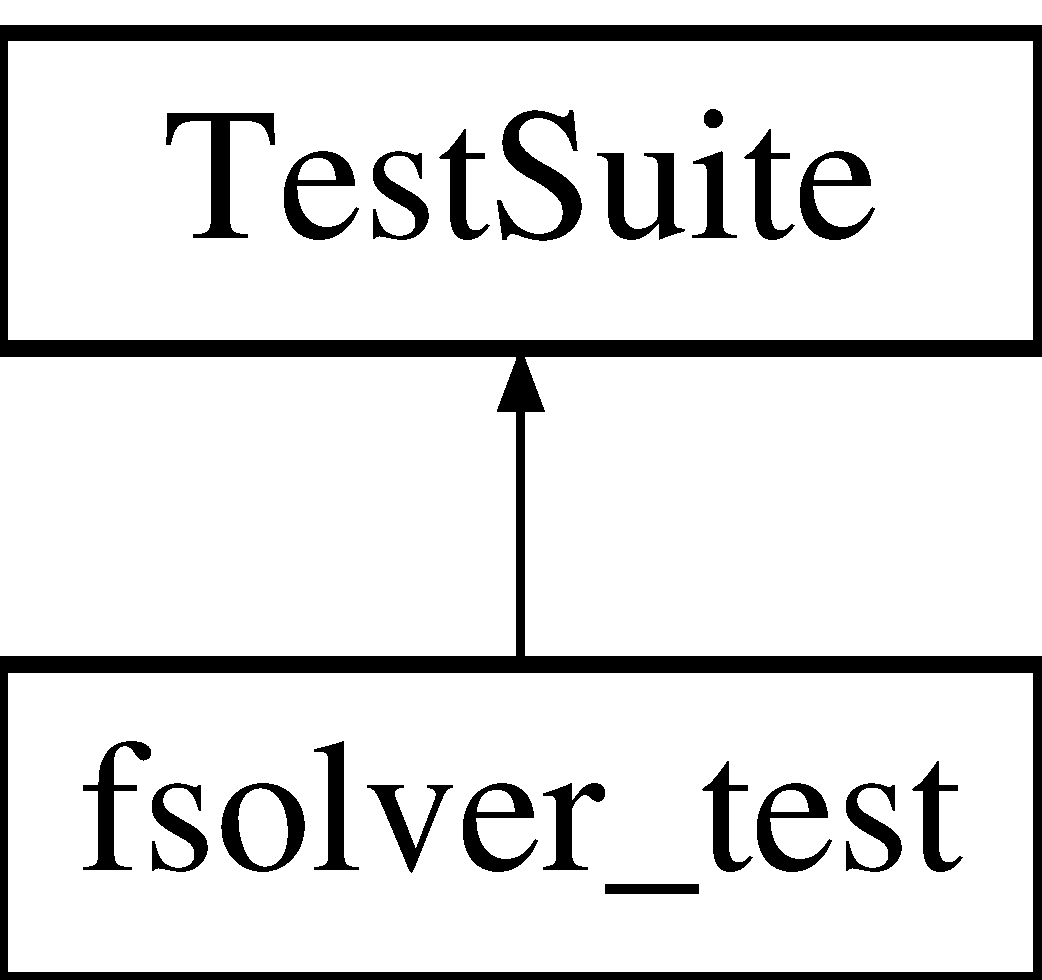
\includegraphics[height=2.000000cm]{classfsolver__test}
\end{center}
\end{figure}
\subsection*{Public Member Functions}
\begin{DoxyCompactItemize}
\item 
void {\bf test\-Fsolver\-\_\-eigenvalue} (void)
\item 
void {\bf test\-Fsolver\-\_\-same\-Input} (void)
\item 
void {\bf test\-Fsolver\-\_\-supersonicproblem} (void)
\item 
void {\bf test\-Fsolver\-\_\-\-Netupdate\-Left} (void)
\item 
void {\bf test\-Fsolver\-\_\-overload\-Function} (void)
\end{DoxyCompactItemize}


\subsection{Detailed Description}
Test class for fsolver implementation. This file contains serveral tests for task 1.\-4 and 2.\-3 

\subsection{Member Function Documentation}
\index{fsolver\-\_\-test@{fsolver\-\_\-test}!test\-Fsolver\-\_\-eigenvalue@{test\-Fsolver\-\_\-eigenvalue}}
\index{test\-Fsolver\-\_\-eigenvalue@{test\-Fsolver\-\_\-eigenvalue}!fsolver_test@{fsolver\-\_\-test}}
\subsubsection[{test\-Fsolver\-\_\-eigenvalue}]{\setlength{\rightskip}{0pt plus 5cm}void fsolver\-\_\-test\-::test\-Fsolver\-\_\-eigenvalue (
\begin{DoxyParamCaption}
\item[{void}]{}
\end{DoxyParamCaption}
)\hspace{0.3cm}{\ttfamily [inline]}}\label{classfsolver__test_a9ee19f26b6d89b40a9ca8d8297b21ef6}
Testing fsolver with calculated values \index{fsolver\-\_\-test@{fsolver\-\_\-test}!test\-Fsolver\-\_\-\-Netupdate\-Left@{test\-Fsolver\-\_\-\-Netupdate\-Left}}
\index{test\-Fsolver\-\_\-\-Netupdate\-Left@{test\-Fsolver\-\_\-\-Netupdate\-Left}!fsolver_test@{fsolver\-\_\-test}}
\subsubsection[{test\-Fsolver\-\_\-\-Netupdate\-Left}]{\setlength{\rightskip}{0pt plus 5cm}void fsolver\-\_\-test\-::test\-Fsolver\-\_\-\-Netupdate\-Left (
\begin{DoxyParamCaption}
\item[{void}]{}
\end{DoxyParamCaption}
)\hspace{0.3cm}{\ttfamily [inline]}}\label{classfsolver__test_a29112a3593900fcf17c582a885f47e31}
Testing fsolver for Task 2 Testing netupdate and max\-Edge\-Speed with calculated values. \index{fsolver\-\_\-test@{fsolver\-\_\-test}!test\-Fsolver\-\_\-overload\-Function@{test\-Fsolver\-\_\-overload\-Function}}
\index{test\-Fsolver\-\_\-overload\-Function@{test\-Fsolver\-\_\-overload\-Function}!fsolver_test@{fsolver\-\_\-test}}
\subsubsection[{test\-Fsolver\-\_\-overload\-Function}]{\setlength{\rightskip}{0pt plus 5cm}void fsolver\-\_\-test\-::test\-Fsolver\-\_\-overload\-Function (
\begin{DoxyParamCaption}
\item[{void}]{}
\end{DoxyParamCaption}
)\hspace{0.3cm}{\ttfamily [inline]}}\label{classfsolver__test_ab69baea0d5516afd3620724a42b4d223}
Cxxtests for overloaded function \index{fsolver\-\_\-test@{fsolver\-\_\-test}!test\-Fsolver\-\_\-same\-Input@{test\-Fsolver\-\_\-same\-Input}}
\index{test\-Fsolver\-\_\-same\-Input@{test\-Fsolver\-\_\-same\-Input}!fsolver_test@{fsolver\-\_\-test}}
\subsubsection[{test\-Fsolver\-\_\-same\-Input}]{\setlength{\rightskip}{0pt plus 5cm}void fsolver\-\_\-test\-::test\-Fsolver\-\_\-same\-Input (
\begin{DoxyParamCaption}
\item[{void}]{}
\end{DoxyParamCaption}
)\hspace{0.3cm}{\ttfamily [inline]}}\label{classfsolver__test_a1f1e202106dd97f295aa4c3a2b826cdd}
Testing fsolver with same inputs. left\-\_\-h == right\-\_\-h left\-\_\-hu == right\-\_\-hu \index{fsolver\-\_\-test@{fsolver\-\_\-test}!test\-Fsolver\-\_\-supersonicproblem@{test\-Fsolver\-\_\-supersonicproblem}}
\index{test\-Fsolver\-\_\-supersonicproblem@{test\-Fsolver\-\_\-supersonicproblem}!fsolver_test@{fsolver\-\_\-test}}
\subsubsection[{test\-Fsolver\-\_\-supersonicproblem}]{\setlength{\rightskip}{0pt plus 5cm}void fsolver\-\_\-test\-::test\-Fsolver\-\_\-supersonicproblem (
\begin{DoxyParamCaption}
\item[{void}]{}
\end{DoxyParamCaption}
)\hspace{0.3cm}{\ttfamily [inline]}}\label{classfsolver__test_a094e58fc97459a59c94a5796a7a87846}
Supersonic problem

lambda1\-\_\-roe \&\& lambda2\-\_\-roe $<$ 0 =$>$ left\-\_\-wavespeed = lambda1\-\_\-roe right\-\_\-wavespeed = 0

lambda2\-\_\-roe \&\& lambda2\-\_\-roe $>$ 0 =$>$ left\-\_\-wavespeed = 0 right\-\_\-wavespeed = lambda2\-\_\-roe 

The documentation for this class was generated from the following file\-:\begin{DoxyCompactItemize}
\item 
src/solvers/fsolver\-\_\-test.\-h\end{DoxyCompactItemize}

\section{tools\-:\-:Logger Class Reference}
\label{classtools_1_1Logger}\index{tools\-::\-Logger@{tools\-::\-Logger}}
\subsection*{Public Member Functions}
\begin{DoxyCompactItemize}
\item 
{\bf Logger} (const int i\-\_\-process\-Rank=0, const std\-::string i\-\_\-program\-Name=\char`\"{}S\-W\-E\char`\"{}, const std\-::string i\-\_\-welcome\-Message=\char`\"{}Welcome to\char`\"{}, const std\-::string i\-\_\-copy\-Rights=\char`\"{}\textbackslash{}n\textbackslash{}n\-S\-W\-E Copyright (C) 2012-\/2013\textbackslash{}n\char`\"{}\char`\"{}  Technische Universitaet Muenchen\textbackslash{}n\char`\"{}\char`\"{}  Department of Informatics\textbackslash{}n\char`\"{}\char`\"{}  Chair of Scientific Computing\textbackslash{}n\char`\"{}\char`\"{}  http\-://www5.\-in.\-tum.\-de/S\-W\-E\textbackslash{}n\char`\"{}\char`\"{}\textbackslash{}n\char`\"{}\char`\"{}S\-W\-E comes with A\-B\-S\-O\-L\-U\-T\-E\-L\-Y N\-O W\-A\-R\-R\-A\-N\-T\-Y.\textbackslash{}n\char`\"{}\char`\"{}S\-W\-E is free software, and you are welcome to redistribute it\textbackslash{}n\char`\"{}\char`\"{}under certain conditions.\textbackslash{}n\char`\"{}\char`\"{}Details can be found in the file \textbackslash{}'gpl.\-txt\textbackslash{}'.\char`\"{}, const std\-::string i\-\_\-finish\-Message=\char`\"{}finished successfully.\char`\"{}, const std\-::string i\-\_\-mid\-Delimiter=\char`\"{}\textbackslash{}n-\/-\/-\/-\/-\/-\/-\/-\/-\/-\/-\/-\/-\/-\/-\/-\/-\/-\/-\/-\/-\/-\/-\/-\/-\/-\/-\/-\/-\/-\/-\/-\/-\/-\/-\/-\/-\/-\/-\/-\/-\/-\/-\/-\/-\/-\/-\/-\/-\/-\/-\/-\/-\/-\/-\/-\/-\/-\/-\/-\/-\/-\/-\/-\/-\/-\/\textbackslash{}n\char`\"{}, const std\-::string i\-\_\-large\-Delimiter=\char`\"{}\textbackslash{}n$\ast$$\ast$$\ast$$\ast$$\ast$$\ast$$\ast$$\ast$$\ast$$\ast$$\ast$$\ast$$\ast$$\ast$$\ast$$\ast$$\ast$$\ast$$\ast$$\ast$$\ast$$\ast$$\ast$$\ast$$\ast$$\ast$$\ast$$\ast$$\ast$$\ast$$\ast$$\ast$$\ast$$\ast$$\ast$$\ast$$\ast$$\ast$$\ast$$\ast$$\ast$$\ast$$\ast$$\ast$$\ast$$\ast$$\ast$$\ast$$\ast$$\ast$$\ast$$\ast$$\ast$$\ast$$\ast$$\ast$$\ast$$\ast$$\ast$$\ast$$\ast$\textbackslash{}n\char`\"{}, const std\-::string i\-\_\-indentation=\char`\"{}\textbackslash{}t\char`\"{})
\item 
virtual {\bf $\sim$\-Logger} ()
\item 
void {\bf print\-Welcome\-Message} ()
\item 
void {\bf print\-Finish\-Message} ()
\item 
std\-::ostream \& {\bf cout} ()
\item 
void {\bf set\-Process\-Rank} (const int i\-\_\-process\-Rank)
\item 
void {\bf print\-String} (const std\-::string i\-\_\-string)
\item 
void {\bf print\-Number\-Of\-Processes} (const int i\-\_\-number\-Of\-Processes, const std\-::string i\-\_\-processes\-Name=\char`\"{}M\-P\-I processes\char`\"{})
\item 
void {\bf print\-Number\-Of\-Cells} (const int i\-\_\-n\-X, const int i\-\_\-n\-Y, const std\-::string i\-\_\-cell\-Message=\char`\"{}cells\char`\"{})
\item 
void {\bf print\-Number\-Of\-Cells\-Per\-Process} (const int i\-\_\-n\-X, const int i\-\_\-n\-Y)
\item 
void {\bf print\-Cell\-Size} (const float i\-\_\-d\-X, const float i\-\_\-d\-Y, const std\-::string i\-\_\-unit=\char`\"{}m\char`\"{})
\item 
void {\bf print\-Number\-Of\-Blocks} (const int i\-\_\-n\-X, const int i\-\_\-n\-Y)
\item 
void {\bf print\-Start\-Message} (const std\-::string i\-\_\-start\-Message=\char`\"{}Everything is set up, starting the simulation.\char`\"{})
\item 
void {\bf print\-Simulation\-Time} (const float i\-\_\-time, const std\-::string i\-\_\-simulation\-Time\-Message=\char`\"{}Simulation at time\char`\"{})
\item 
void {\bf print\-Output\-File\-Creation} (const std\-::string i\-\_\-file\-Name, const int i\-\_\-block\-X, const int i\-\_\-block\-Y, const std\-::string i\-\_\-file\-Type=\char`\"{}net\-C\-D\-F\char`\"{})
\item 
void {\bf print\-Output\-Time} (const float i\-\_\-time, const std\-::string i\-\_\-output\-Time\-Message=\char`\"{}Writing output file at time\char`\"{})
\item 
void {\bf print\-Statistics\-Message} (const std\-::string i\-\_\-statistics\-Message=\char`\"{}Simulation finished. Printing statistics for each process.\char`\"{})
\item 
void {\bf print\-Solver\-Statistics} (const long i\-\_\-first\-Solver\-Counter, const long i\-\_\-second\-Solver\-Counter, const int i\-\_\-block\-X=0, const int i\-\_\-block\-Y=0, const std\-::string i\-\_\-first\-Solver\-Name=\char`\"{}f-\/Wave solver\char`\"{}, const std\-::string i\-\_\-second\-Solver\-Name=\char`\"{}Augemented Riemann solver\char`\"{})
\item 
void {\bf update\-Time} (const std\-::string \&i\-\_\-name)
\item 
void {\bf reset\-Clock\-To\-Current\-Time} (const std\-::string \&i\-\_\-name)
\item 
void {\bf init\-Wall\-Clock\-Time} (const double i\-\_\-wall\-Clock\-Time)
\item 
void {\bf print\-Wall\-Clock\-Time} (const double i\-\_\-wall\-Clock\-Time, const std\-::string i\-\_\-wall\-Clock\-Time\-Message=\char`\"{}wall clock time\char`\"{})
\item 
void {\bf print\-Time} (const std\-::string \&i\-\_\-name, const std\-::string \&i\-\_\-message)
\item 
double {\bf get\-Time} (const std\-::string \&i\-\_\-name)
\item 
void {\bf print\-Iterations\-Done} (unsigned int i\-\_\-iterations, std\-::string i\-\_\-iteration\-Message=\char`\"{}iterations done\char`\"{})
\item 
void {\bf print\-Element\-Updates\-Done} (unsigned int i\-\_\-iterations, const int i\-\_\-n\-X, const int i\-\_\-n\-Y, const std\-::string \&i\-\_\-name, const std\-::string i\-\_\-iteration\-Message=\char`\"{}element updates per second done\char`\"{})
\end{DoxyCompactItemize}
\subsection*{Static Public Attributes}
\begin{DoxyCompactItemize}
\item 
static {\bf Logger} {\bf logger}
\end{DoxyCompactItemize}


\subsection{Constructor \& Destructor Documentation}
\index{tools\-::\-Logger@{tools\-::\-Logger}!Logger@{Logger}}
\index{Logger@{Logger}!tools::Logger@{tools\-::\-Logger}}
\subsubsection[{Logger}]{\setlength{\rightskip}{0pt plus 5cm}tools\-::\-Logger\-::\-Logger (
\begin{DoxyParamCaption}
\item[{const int}]{i\-\_\-process\-Rank = {\ttfamily 0}, }
\item[{const std\-::string}]{i\-\_\-program\-Name = {\ttfamily \char`\"{}SWE\char`\"{}}, }
\item[{const std\-::string}]{i\-\_\-welcome\-Message = {\ttfamily \char`\"{}Welcome~to\char`\"{}}, }
\item[{const std\-::string}]{i\-\_\-copy\-Rights = {\ttfamily \char`\"{}\textbackslash{}n\textbackslash{}nSWE~Copyright~(C)~2012-\/2013\textbackslash{}n\char`\"{}~\char`\"{}~~Technische~Universitaet~Muenchen\textbackslash{}n\char`\"{}~\char`\"{}~~Department~of~Informatics\textbackslash{}n\char`\"{}~\char`\"{}~~Chair~of~Scientific~Computing\textbackslash{}n\char`\"{}~\char`\"{}~~http\-://www5.in.tum.de/SWE\textbackslash{}n\char`\"{}~\char`\"{}\textbackslash{}n\char`\"{}~\char`\"{}SWE~comes~with~ABSOLUTELY~NO~WARRANTY.\textbackslash{}n\char`\"{}~\char`\"{}SWE~is~free~software,~and~you~are~welcome~to~redistribute~it\textbackslash{}n\char`\"{}~\char`\"{}under~certain~conditions.\textbackslash{}n\char`\"{}~\char`\"{}Details~can~be~found~in~the~file~\textbackslash{}'gpl.txt\textbackslash{}'.\char`\"{}}, }
\item[{const std\-::string}]{i\-\_\-finish\-Message = {\ttfamily \char`\"{}finished~successfully.\char`\"{}}, }
\item[{const std\-::string}]{i\-\_\-mid\-Delimiter = {\ttfamily \char`\"{}\textbackslash{}n-\/-\/-\/-\/-\/-\/-\/-\/-\/-\/-\/-\/-\/-\/-\/-\/-\/-\/-\/-\/-\/-\/-\/-\/-\/-\/-\/-\/-\/-\/-\/-\/-\/-\/-\/-\/-\/-\/-\/-\/-\/-\/-\/-\/-\/-\/-\/-\/-\/-\/-\/-\/-\/-\/-\/-\/-\/-\/-\/-\/-\/-\/-\/-\/-\/-\/\textbackslash{}n\char`\"{}}, }
\item[{const std\-::string}]{i\-\_\-large\-Delimiter = {\ttfamily \char`\"{}\textbackslash{}n$\ast$$\ast$$\ast$$\ast$$\ast$$\ast$$\ast$$\ast$$\ast$$\ast$$\ast$$\ast$$\ast$$\ast$$\ast$$\ast$$\ast$$\ast$$\ast$$\ast$$\ast$$\ast$$\ast$$\ast$$\ast$$\ast$$\ast$$\ast$$\ast$$\ast$$\ast$$\ast$$\ast$$\ast$$\ast$$\ast$$\ast$$\ast$$\ast$$\ast$$\ast$$\ast$$\ast$$\ast$$\ast$$\ast$$\ast$$\ast$$\ast$$\ast$$\ast$$\ast$$\ast$$\ast$$\ast$$\ast$$\ast$$\ast$$\ast$$\ast$$\ast$\textbackslash{}n\char`\"{}}, }
\item[{const std\-::string}]{i\-\_\-indentation = {\ttfamily \char`\"{}\textbackslash{}t\char`\"{}}}
\end{DoxyParamCaption}
)\hspace{0.3cm}{\ttfamily [inline]}}\label{classtools_1_1Logger_a9e1e0651776fcc78f89a1a1dcf339249}
The Constructor. Prints the welcome message (process rank 0 only).


\begin{DoxyParams}{Parameters}
{\em i\-\_\-process\-Rank} & rank of the constructing process. \\
\hline
{\em i\-\_\-program\-Name} & definition of the program name. \\
\hline
{\em i\-\_\-welcome\-Message} & definition of the welcome message. \\
\hline
{\em i\-\_\-start\-Message} & definition of the start message. \\
\hline
{\em i\-\_\-simulation\-Time\-Message} & definition of the simulation time message. \\
\hline
{\em i\-\_\-execution\-Time\-Message} & definition of the execution time message. \\
\hline
{\em i\-\_\-cpu\-Time\-Message} & definition of the C\-P\-U time message. \\
\hline
{\em i\-\_\-finish\-Message} & definition of the finish message. \\
\hline
{\em i\-\_\-mid\-Delimiter} & definition of the mid-\/size delimiter. \\
\hline
{\em i\-\_\-large\-Delimiter} & definition of the large delimiter. \\
\hline
{\em i\-\_\-indentation} & definition of the indentation (used in all messages, except welcome, start and finish). \\
\hline
\end{DoxyParams}
\index{tools\-::\-Logger@{tools\-::\-Logger}!$\sim$\-Logger@{$\sim$\-Logger}}
\index{$\sim$\-Logger@{$\sim$\-Logger}!tools::Logger@{tools\-::\-Logger}}
\subsubsection[{$\sim$\-Logger}]{\setlength{\rightskip}{0pt plus 5cm}virtual tools\-::\-Logger\-::$\sim$\-Logger (
\begin{DoxyParamCaption}
{}
\end{DoxyParamCaption}
)\hspace{0.3cm}{\ttfamily [inline]}, {\ttfamily [virtual]}}\label{classtools_1_1Logger_a58f170bf361ba7ceb3a4e0d9ec36bdf5}
The Destructor. Prints the finish message (process rank 0 only). 

\subsection{Member Function Documentation}
\index{tools\-::\-Logger@{tools\-::\-Logger}!cout@{cout}}
\index{cout@{cout}!tools::Logger@{tools\-::\-Logger}}
\subsubsection[{cout}]{\setlength{\rightskip}{0pt plus 5cm}std\-::ostream\& tools\-::\-Logger\-::cout (
\begin{DoxyParamCaption}
{}
\end{DoxyParamCaption}
)\hspace{0.3cm}{\ttfamily [inline]}}\label{classtools_1_1Logger_ab0d82d23125a3d5d8b737984e678f43a}
Default output stream of the logger.

\begin{DoxyReturn}{Returns}
extended (time + indentation) std\-::cout stream. 
\end{DoxyReturn}
\index{tools\-::\-Logger@{tools\-::\-Logger}!get\-Time@{get\-Time}}
\index{get\-Time@{get\-Time}!tools::Logger@{tools\-::\-Logger}}
\subsubsection[{get\-Time}]{\setlength{\rightskip}{0pt plus 5cm}double tools\-::\-Logger\-::get\-Time (
\begin{DoxyParamCaption}
\item[{const std\-::string \&}]{i\-\_\-name}
\end{DoxyParamCaption}
)\hspace{0.3cm}{\ttfamily [inline]}}\label{classtools_1_1Logger_a01a480f7c6ce911114529b193188f211}
Get elapsed time


\begin{DoxyParams}{Parameters}
{\em i\-\_\-name} & Name of the time \\
\hline
\end{DoxyParams}
\begin{DoxyReturn}{Returns}
elapsed time 
\end{DoxyReturn}
\index{tools\-::\-Logger@{tools\-::\-Logger}!init\-Wall\-Clock\-Time@{init\-Wall\-Clock\-Time}}
\index{init\-Wall\-Clock\-Time@{init\-Wall\-Clock\-Time}!tools::Logger@{tools\-::\-Logger}}
\subsubsection[{init\-Wall\-Clock\-Time}]{\setlength{\rightskip}{0pt plus 5cm}void tools\-::\-Logger\-::init\-Wall\-Clock\-Time (
\begin{DoxyParamCaption}
\item[{const double}]{i\-\_\-wall\-Clock\-Time}
\end{DoxyParamCaption}
)\hspace{0.3cm}{\ttfamily [inline]}}\label{classtools_1_1Logger_ab1bb09a74580560b36c19979d88ef3bc}
Initialize the wall clock time.


\begin{DoxyParams}{Parameters}
{\em i\-\_\-wall\-Clock\-Time} & value the wall block time will be set to. \\
\hline
\end{DoxyParams}
\index{tools\-::\-Logger@{tools\-::\-Logger}!print\-Cell\-Size@{print\-Cell\-Size}}
\index{print\-Cell\-Size@{print\-Cell\-Size}!tools::Logger@{tools\-::\-Logger}}
\subsubsection[{print\-Cell\-Size}]{\setlength{\rightskip}{0pt plus 5cm}void tools\-::\-Logger\-::print\-Cell\-Size (
\begin{DoxyParamCaption}
\item[{const float}]{i\-\_\-d\-X, }
\item[{const float}]{i\-\_\-d\-Y, }
\item[{const std\-::string}]{i\-\_\-unit = {\ttfamily \char`\"{}m\char`\"{}}}
\end{DoxyParamCaption}
)\hspace{0.3cm}{\ttfamily [inline]}}\label{classtools_1_1Logger_a4c81063c055f072c465853d6da85743b}
Print the size of a cell


\begin{DoxyParams}{Parameters}
{\em i\-\_\-d\-X} & size in x-\/direction. \\
\hline
{\em i\-\_\-d\-Y} & size in y-\/direction. \\
\hline
{\em i\-\_\-unit} & measurement unit. \\
\hline
\end{DoxyParams}
\index{tools\-::\-Logger@{tools\-::\-Logger}!print\-Element\-Updates\-Done@{print\-Element\-Updates\-Done}}
\index{print\-Element\-Updates\-Done@{print\-Element\-Updates\-Done}!tools::Logger@{tools\-::\-Logger}}
\subsubsection[{print\-Element\-Updates\-Done}]{\setlength{\rightskip}{0pt plus 5cm}void tools\-::\-Logger\-::print\-Element\-Updates\-Done (
\begin{DoxyParamCaption}
\item[{unsigned int}]{i\-\_\-iterations, }
\item[{const int}]{i\-\_\-n\-X, }
\item[{const int}]{i\-\_\-n\-Y, }
\item[{const std\-::string \&}]{i\-\_\-name, }
\item[{const std\-::string}]{i\-\_\-iteration\-Message = {\ttfamily \char`\"{}element~updates~per~second~done\char`\"{}}}
\end{DoxyParamCaption}
)\hspace{0.3cm}{\ttfamily [inline]}}\label{classtools_1_1Logger_aff8aabe69fd994258cf5238ff0e1f55f}
Print number of element updates done


\begin{DoxyParams}{Parameters}
{\em i\-\_\-iterations} & Number of iterations done \\
\hline
{\em i\-\_\-interation\-Message} & Iterations done message \\
\hline
\end{DoxyParams}
\index{tools\-::\-Logger@{tools\-::\-Logger}!print\-Finish\-Message@{print\-Finish\-Message}}
\index{print\-Finish\-Message@{print\-Finish\-Message}!tools::Logger@{tools\-::\-Logger}}
\subsubsection[{print\-Finish\-Message}]{\setlength{\rightskip}{0pt plus 5cm}void tools\-::\-Logger\-::print\-Finish\-Message (
\begin{DoxyParamCaption}
{}
\end{DoxyParamCaption}
)\hspace{0.3cm}{\ttfamily [inline]}}\label{classtools_1_1Logger_a539d6f7c8e60c0ee887912c92c1dfa5c}
Print the finish message. \index{tools\-::\-Logger@{tools\-::\-Logger}!print\-Iterations\-Done@{print\-Iterations\-Done}}
\index{print\-Iterations\-Done@{print\-Iterations\-Done}!tools::Logger@{tools\-::\-Logger}}
\subsubsection[{print\-Iterations\-Done}]{\setlength{\rightskip}{0pt plus 5cm}void tools\-::\-Logger\-::print\-Iterations\-Done (
\begin{DoxyParamCaption}
\item[{unsigned int}]{i\-\_\-iterations, }
\item[{std\-::string}]{i\-\_\-iteration\-Message = {\ttfamily \char`\"{}iterations~done\char`\"{}}}
\end{DoxyParamCaption}
)\hspace{0.3cm}{\ttfamily [inline]}}\label{classtools_1_1Logger_a2e9f836ab40bfde976770aa711b8547d}
Print number of iterations done


\begin{DoxyParams}{Parameters}
{\em i\-\_\-iterations} & Number of iterations done \\
\hline
{\em i\-\_\-interation\-Message} & Iterations done message \\
\hline
\end{DoxyParams}
\index{tools\-::\-Logger@{tools\-::\-Logger}!print\-Number\-Of\-Blocks@{print\-Number\-Of\-Blocks}}
\index{print\-Number\-Of\-Blocks@{print\-Number\-Of\-Blocks}!tools::Logger@{tools\-::\-Logger}}
\subsubsection[{print\-Number\-Of\-Blocks}]{\setlength{\rightskip}{0pt plus 5cm}void tools\-::\-Logger\-::print\-Number\-Of\-Blocks (
\begin{DoxyParamCaption}
\item[{const int}]{i\-\_\-n\-X, }
\item[{const int}]{i\-\_\-n\-Y}
\end{DoxyParamCaption}
)\hspace{0.3cm}{\ttfamily [inline]}}\label{classtools_1_1Logger_a6c71eab182524a84037eb6fe1ac42e9e}
Print the number of defined blocks. (process rank 0 only)


\begin{DoxyParams}{Parameters}
{\em i\-\_\-n\-X} & number of blocks in x-\/direction. \\
\hline
{\em i\-\_\-n\-Y} & number of blocks in y-\/direction. \\
\hline
\end{DoxyParams}
\index{tools\-::\-Logger@{tools\-::\-Logger}!print\-Number\-Of\-Cells@{print\-Number\-Of\-Cells}}
\index{print\-Number\-Of\-Cells@{print\-Number\-Of\-Cells}!tools::Logger@{tools\-::\-Logger}}
\subsubsection[{print\-Number\-Of\-Cells}]{\setlength{\rightskip}{0pt plus 5cm}void tools\-::\-Logger\-::print\-Number\-Of\-Cells (
\begin{DoxyParamCaption}
\item[{const int}]{i\-\_\-n\-X, }
\item[{const int}]{i\-\_\-n\-Y, }
\item[{const std\-::string}]{i\-\_\-cell\-Message = {\ttfamily \char`\"{}cells\char`\"{}}}
\end{DoxyParamCaption}
)\hspace{0.3cm}{\ttfamily [inline]}}\label{classtools_1_1Logger_a2da0a6c575304e91bea546dddc94f72d}
Print the number of cells. (process rank 0 only)


\begin{DoxyParams}{Parameters}
{\em i\-\_\-n\-X} & number of cells in x-\/direction. \\
\hline
{\em i\-\_\-n\-Y} & number of cells in y-\/direction. \\
\hline
{\em i\-\_\-cell\-Message} & cell message. \\
\hline
\end{DoxyParams}
\index{tools\-::\-Logger@{tools\-::\-Logger}!print\-Number\-Of\-Cells\-Per\-Process@{print\-Number\-Of\-Cells\-Per\-Process}}
\index{print\-Number\-Of\-Cells\-Per\-Process@{print\-Number\-Of\-Cells\-Per\-Process}!tools::Logger@{tools\-::\-Logger}}
\subsubsection[{print\-Number\-Of\-Cells\-Per\-Process}]{\setlength{\rightskip}{0pt plus 5cm}void tools\-::\-Logger\-::print\-Number\-Of\-Cells\-Per\-Process (
\begin{DoxyParamCaption}
\item[{const int}]{i\-\_\-n\-X, }
\item[{const int}]{i\-\_\-n\-Y}
\end{DoxyParamCaption}
)\hspace{0.3cm}{\ttfamily [inline]}}\label{classtools_1_1Logger_acf2b4547c8b138e4e8e338002687a149}
Print the number of cells per Process.


\begin{DoxyParams}{Parameters}
{\em i\-\_\-n\-X} & number of cells in x-\/direction. \\
\hline
{\em i\-\_\-n\-Y} & number of cells in y-\/direction. \\
\hline
\end{DoxyParams}
\index{tools\-::\-Logger@{tools\-::\-Logger}!print\-Number\-Of\-Processes@{print\-Number\-Of\-Processes}}
\index{print\-Number\-Of\-Processes@{print\-Number\-Of\-Processes}!tools::Logger@{tools\-::\-Logger}}
\subsubsection[{print\-Number\-Of\-Processes}]{\setlength{\rightskip}{0pt plus 5cm}void tools\-::\-Logger\-::print\-Number\-Of\-Processes (
\begin{DoxyParamCaption}
\item[{const int}]{i\-\_\-number\-Of\-Processes, }
\item[{const std\-::string}]{i\-\_\-processes\-Name = {\ttfamily \char`\"{}MPI~processes\char`\"{}}}
\end{DoxyParamCaption}
)\hspace{0.3cm}{\ttfamily [inline]}}\label{classtools_1_1Logger_a89b9dfd5340a4e18d7b8f1225d996730}
Print the number of processes. (process rank 0 only)


\begin{DoxyParams}{Parameters}
{\em i\-\_\-number\-Of\-Processes} & number of processes. \\
\hline
{\em i\-\_\-processes\-Name} & name of the processes. \\
\hline
\end{DoxyParams}
\index{tools\-::\-Logger@{tools\-::\-Logger}!print\-Output\-File\-Creation@{print\-Output\-File\-Creation}}
\index{print\-Output\-File\-Creation@{print\-Output\-File\-Creation}!tools::Logger@{tools\-::\-Logger}}
\subsubsection[{print\-Output\-File\-Creation}]{\setlength{\rightskip}{0pt plus 5cm}void tools\-::\-Logger\-::print\-Output\-File\-Creation (
\begin{DoxyParamCaption}
\item[{const std\-::string}]{i\-\_\-file\-Name, }
\item[{const int}]{i\-\_\-block\-X, }
\item[{const int}]{i\-\_\-block\-Y, }
\item[{const std\-::string}]{i\-\_\-file\-Type = {\ttfamily \char`\"{}netCDF\char`\"{}}}
\end{DoxyParamCaption}
)\hspace{0.3cm}{\ttfamily [inline]}}\label{classtools_1_1Logger_aec0d76a09748963c9f0b68239e4499c0}
Print the creation of an output file.


\begin{DoxyParams}{Parameters}
{\em i\-\_\-file\-Name} & name of the file. \\
\hline
{\em i\-\_\-block\-X} & block position in x-\/direction. \\
\hline
{\em i\-\_\-block\-Y} & block position in y-\/direction. \\
\hline
{\em i\-\_\-file\-Type} & type of the output file. \\
\hline
\end{DoxyParams}
\index{tools\-::\-Logger@{tools\-::\-Logger}!print\-Output\-Time@{print\-Output\-Time}}
\index{print\-Output\-Time@{print\-Output\-Time}!tools::Logger@{tools\-::\-Logger}}
\subsubsection[{print\-Output\-Time}]{\setlength{\rightskip}{0pt plus 5cm}void tools\-::\-Logger\-::print\-Output\-Time (
\begin{DoxyParamCaption}
\item[{const float}]{i\-\_\-time, }
\item[{const std\-::string}]{i\-\_\-output\-Time\-Message = {\ttfamily \char`\"{}Writing~output~file~at~time\char`\"{}}}
\end{DoxyParamCaption}
)\hspace{0.3cm}{\ttfamily [inline]}}\label{classtools_1_1Logger_ab7f380c82631174ff826dfd8bf519058}
Print the current output time.


\begin{DoxyParams}{Parameters}
{\em i\-\_\-time} & time in seconds. \\
\hline
{\em i\-\_\-output\-Time\-Message} & output message. \\
\hline
\end{DoxyParams}
\index{tools\-::\-Logger@{tools\-::\-Logger}!print\-Simulation\-Time@{print\-Simulation\-Time}}
\index{print\-Simulation\-Time@{print\-Simulation\-Time}!tools::Logger@{tools\-::\-Logger}}
\subsubsection[{print\-Simulation\-Time}]{\setlength{\rightskip}{0pt plus 5cm}void tools\-::\-Logger\-::print\-Simulation\-Time (
\begin{DoxyParamCaption}
\item[{const float}]{i\-\_\-time, }
\item[{const std\-::string}]{i\-\_\-simulation\-Time\-Message = {\ttfamily \char`\"{}Simulation~at~time\char`\"{}}}
\end{DoxyParamCaption}
)\hspace{0.3cm}{\ttfamily [inline]}}\label{classtools_1_1Logger_ac829729cc06f2a6e43f0272ada747685}
Print current simulation time. (process rank 0 only)


\begin{DoxyParams}{Parameters}
{\em i\-\_\-time} & time in seconds. \\
\hline
\end{DoxyParams}
\index{tools\-::\-Logger@{tools\-::\-Logger}!print\-Solver\-Statistics@{print\-Solver\-Statistics}}
\index{print\-Solver\-Statistics@{print\-Solver\-Statistics}!tools::Logger@{tools\-::\-Logger}}
\subsubsection[{print\-Solver\-Statistics}]{\setlength{\rightskip}{0pt plus 5cm}void tools\-::\-Logger\-::print\-Solver\-Statistics (
\begin{DoxyParamCaption}
\item[{const long}]{i\-\_\-first\-Solver\-Counter, }
\item[{const long}]{i\-\_\-second\-Solver\-Counter, }
\item[{const int}]{i\-\_\-block\-X = {\ttfamily 0}, }
\item[{const int}]{i\-\_\-block\-Y = {\ttfamily 0}, }
\item[{const std\-::string}]{i\-\_\-first\-Solver\-Name = {\ttfamily \char`\"{}f-\/Wave~solver\char`\"{}}, }
\item[{const std\-::string}]{i\-\_\-second\-Solver\-Name = {\ttfamily \char`\"{}Augemented~Riemann~solver\char`\"{}}}
\end{DoxyParamCaption}
)\hspace{0.3cm}{\ttfamily [inline]}}\label{classtools_1_1Logger_a6f23f0f674d0e7bbf1a52442eff5c031}
Print solver statistics


\begin{DoxyParams}{Parameters}
{\em i\-\_\-first\-Solver\-Counter} & times the first solver was used. \\
\hline
{\em i\-\_\-second\-Solver\-Counter} & times the second solver was used. \\
\hline
{\em i\-\_\-block\-X} & position of the block in x-\/direction \\
\hline
{\em i\-\_\-block\-Y} & position of the block in y-\/direction \\
\hline
{\em i\-\_\-first\-Solver\-Name} & name of the first solver. \\
\hline
{\em i\-\_\-second\-Solver\-Name} & name of the second solver. \\
\hline
\end{DoxyParams}
\index{tools\-::\-Logger@{tools\-::\-Logger}!print\-Start\-Message@{print\-Start\-Message}}
\index{print\-Start\-Message@{print\-Start\-Message}!tools::Logger@{tools\-::\-Logger}}
\subsubsection[{print\-Start\-Message}]{\setlength{\rightskip}{0pt plus 5cm}void tools\-::\-Logger\-::print\-Start\-Message (
\begin{DoxyParamCaption}
\item[{const std\-::string}]{i\-\_\-start\-Message = {\ttfamily \char`\"{}Everything~is~set~up,~starting~the~simulation.\char`\"{}}}
\end{DoxyParamCaption}
)\hspace{0.3cm}{\ttfamily [inline]}}\label{classtools_1_1Logger_a2d54396c65885248374009cb3b18c2da}
Print the start message. (process rank 0 only) \index{tools\-::\-Logger@{tools\-::\-Logger}!print\-Statistics\-Message@{print\-Statistics\-Message}}
\index{print\-Statistics\-Message@{print\-Statistics\-Message}!tools::Logger@{tools\-::\-Logger}}
\subsubsection[{print\-Statistics\-Message}]{\setlength{\rightskip}{0pt plus 5cm}void tools\-::\-Logger\-::print\-Statistics\-Message (
\begin{DoxyParamCaption}
\item[{const std\-::string}]{i\-\_\-statistics\-Message = {\ttfamily \char`\"{}Simulation~finished.~Printing~statistics~for~each~process.\char`\"{}}}
\end{DoxyParamCaption}
)\hspace{0.3cm}{\ttfamily [inline]}}\label{classtools_1_1Logger_a6030321e16a66849dbf237420702a0da}
Print the statics message.


\begin{DoxyParams}{Parameters}
{\em i\-\_\-statistics\-Message} & statistics message. \\
\hline
\end{DoxyParams}
\index{tools\-::\-Logger@{tools\-::\-Logger}!print\-String@{print\-String}}
\index{print\-String@{print\-String}!tools::Logger@{tools\-::\-Logger}}
\subsubsection[{print\-String}]{\setlength{\rightskip}{0pt plus 5cm}void tools\-::\-Logger\-::print\-String (
\begin{DoxyParamCaption}
\item[{const std\-::string}]{i\-\_\-string}
\end{DoxyParamCaption}
)\hspace{0.3cm}{\ttfamily [inline]}}\label{classtools_1_1Logger_a9642689522ece27ca9c908f24f290134}
Print an arbitrary string.


\begin{DoxyParams}{Parameters}
{\em i\-\_\-string} & some string. \\
\hline
\end{DoxyParams}
\index{tools\-::\-Logger@{tools\-::\-Logger}!print\-Time@{print\-Time}}
\index{print\-Time@{print\-Time}!tools::Logger@{tools\-::\-Logger}}
\subsubsection[{print\-Time}]{\setlength{\rightskip}{0pt plus 5cm}void tools\-::\-Logger\-::print\-Time (
\begin{DoxyParamCaption}
\item[{const std\-::string \&}]{i\-\_\-name, }
\item[{const std\-::string \&}]{i\-\_\-message}
\end{DoxyParamCaption}
)\hspace{0.3cm}{\ttfamily [inline]}}\label{classtools_1_1Logger_a538f0d1e94f6a957a8936d663f56859c}
Print elapsed time.


\begin{DoxyParams}{Parameters}
{\em i\-\_\-name} & Name of the timer \\
\hline
{\em i\-\_\-message} & time message. \\
\hline
\end{DoxyParams}
\index{tools\-::\-Logger@{tools\-::\-Logger}!print\-Wall\-Clock\-Time@{print\-Wall\-Clock\-Time}}
\index{print\-Wall\-Clock\-Time@{print\-Wall\-Clock\-Time}!tools::Logger@{tools\-::\-Logger}}
\subsubsection[{print\-Wall\-Clock\-Time}]{\setlength{\rightskip}{0pt plus 5cm}void tools\-::\-Logger\-::print\-Wall\-Clock\-Time (
\begin{DoxyParamCaption}
\item[{const double}]{i\-\_\-wall\-Clock\-Time, }
\item[{const std\-::string}]{i\-\_\-wall\-Clock\-Time\-Message = {\ttfamily \char`\"{}wall~clock~time\char`\"{}}}
\end{DoxyParamCaption}
)\hspace{0.3cm}{\ttfamily [inline]}}\label{classtools_1_1Logger_a432c4dbdbc532bc792cd0d4b30b3b42e}
Print the elapsed wall clock time.


\begin{DoxyParams}{Parameters}
{\em i\-\_\-wall\-Clock\-Time} & wall clock time message. \\
\hline
\end{DoxyParams}
\index{tools\-::\-Logger@{tools\-::\-Logger}!print\-Welcome\-Message@{print\-Welcome\-Message}}
\index{print\-Welcome\-Message@{print\-Welcome\-Message}!tools::Logger@{tools\-::\-Logger}}
\subsubsection[{print\-Welcome\-Message}]{\setlength{\rightskip}{0pt plus 5cm}void tools\-::\-Logger\-::print\-Welcome\-Message (
\begin{DoxyParamCaption}
{}
\end{DoxyParamCaption}
)\hspace{0.3cm}{\ttfamily [inline]}}\label{classtools_1_1Logger_af45e7a1b4e9c33ab9fbb43e18e284eae}
Print the welcome message. \index{tools\-::\-Logger@{tools\-::\-Logger}!reset\-Clock\-To\-Current\-Time@{reset\-Clock\-To\-Current\-Time}}
\index{reset\-Clock\-To\-Current\-Time@{reset\-Clock\-To\-Current\-Time}!tools::Logger@{tools\-::\-Logger}}
\subsubsection[{reset\-Clock\-To\-Current\-Time}]{\setlength{\rightskip}{0pt plus 5cm}void tools\-::\-Logger\-::reset\-Clock\-To\-Current\-Time (
\begin{DoxyParamCaption}
\item[{const std\-::string \&}]{i\-\_\-name}
\end{DoxyParamCaption}
)\hspace{0.3cm}{\ttfamily [inline]}}\label{classtools_1_1Logger_a46e0d98ad67c8ac1d26ff8d695c5fceb}
Reset a clock to the current time


\begin{DoxyParams}{Parameters}
{\em i\-\_\-name} & Name of timer/clock \\
\hline
\end{DoxyParams}
\index{tools\-::\-Logger@{tools\-::\-Logger}!set\-Process\-Rank@{set\-Process\-Rank}}
\index{set\-Process\-Rank@{set\-Process\-Rank}!tools::Logger@{tools\-::\-Logger}}
\subsubsection[{set\-Process\-Rank}]{\setlength{\rightskip}{0pt plus 5cm}void tools\-::\-Logger\-::set\-Process\-Rank (
\begin{DoxyParamCaption}
\item[{const int}]{i\-\_\-process\-Rank}
\end{DoxyParamCaption}
)\hspace{0.3cm}{\ttfamily [inline]}}\label{classtools_1_1Logger_a1d3e0fcc3cb4c58eb486ac3fe14d30b0}
Set the process rank.


\begin{DoxyParams}{Parameters}
{\em i\-\_\-process\-Rank} & process rank. \\
\hline
\end{DoxyParams}
\index{tools\-::\-Logger@{tools\-::\-Logger}!update\-Time@{update\-Time}}
\index{update\-Time@{update\-Time}!tools::Logger@{tools\-::\-Logger}}
\subsubsection[{update\-Time}]{\setlength{\rightskip}{0pt plus 5cm}void tools\-::\-Logger\-::update\-Time (
\begin{DoxyParamCaption}
\item[{const std\-::string \&}]{i\-\_\-name}
\end{DoxyParamCaption}
)\hspace{0.3cm}{\ttfamily [inline]}}\label{classtools_1_1Logger_ad5986d50f6c7bec49b9d07e9b1e7ac1b}
Update a timer


\begin{DoxyParams}{Parameters}
{\em i\-\_\-name} & Name of timer \\
\hline
\end{DoxyParams}


\subsection{Member Data Documentation}
\index{tools\-::\-Logger@{tools\-::\-Logger}!logger@{logger}}
\index{logger@{logger}!tools::Logger@{tools\-::\-Logger}}
\subsubsection[{logger}]{\setlength{\rightskip}{0pt plus 5cm}{\bf tools\-::\-Logger} tools\-::\-Logger\-::logger\hspace{0.3cm}{\ttfamily [static]}}\label{classtools_1_1Logger_a341eaab3865b60362db6736c2e2b7c68}
The logger all classes should use 

The documentation for this class was generated from the following files\-:\begin{DoxyCompactItemize}
\item 
src/tools/{\bf Logger.\-hh}\item 
src/tools/{\bf Logger.\-cpp}\end{DoxyCompactItemize}

\section{io\-:\-:Net\-Cdf\-Writer Class Reference}
\label{classio_1_1NetCdfWriter}\index{io\-::\-Net\-Cdf\-Writer@{io\-::\-Net\-Cdf\-Writer}}
Inheritance diagram for io\-:\-:Net\-Cdf\-Writer\-:\begin{figure}[H]
\begin{center}
\leavevmode
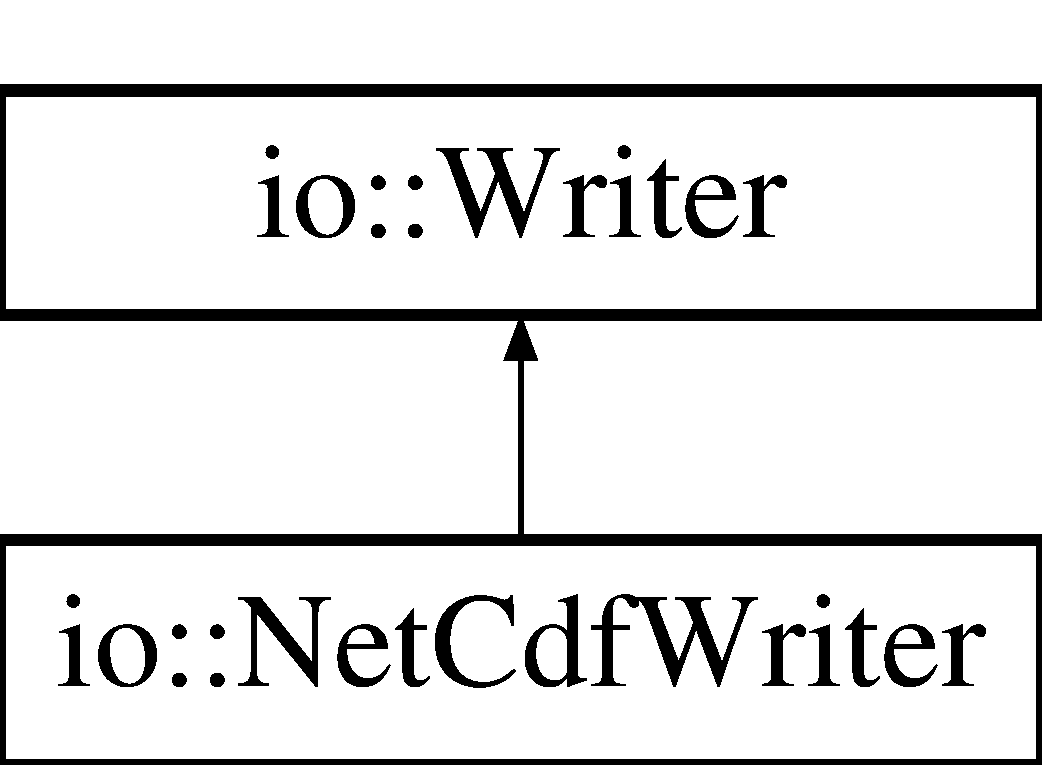
\includegraphics[height=2.000000cm]{classio_1_1NetCdfWriter}
\end{center}
\end{figure}
\subsection*{Public Member Functions}
\begin{DoxyCompactItemize}
\item 
{\bf Net\-Cdf\-Writer} (const std\-::string \&i\-\_\-file\-Name, const {\bf Float2\-D} \&i\-\_\-b, const {\bf Boundary\-Size} \&i\-\_\-boundary\-Size, int i\-\_\-n\-X, int i\-\_\-n\-Y, float i\-\_\-d\-X, float i\-\_\-d\-Y, float i\-\_\-origin\-X=0., float i\-\_\-origin\-Y=0., unsigned int i\-\_\-flush=0)
\item 
virtual {\bf $\sim$\-Net\-Cdf\-Writer} ()
\item 
void {\bf write\-Time\-Step} (const {\bf Float2\-D} \&i\-\_\-h, const {\bf Float2\-D} \&i\-\_\-hu, const {\bf Float2\-D} \&i\-\_\-hv, float i\-\_\-time)
\end{DoxyCompactItemize}
\subsection*{Additional Inherited Members}


\subsection{Constructor \& Destructor Documentation}
\index{io\-::\-Net\-Cdf\-Writer@{io\-::\-Net\-Cdf\-Writer}!Net\-Cdf\-Writer@{Net\-Cdf\-Writer}}
\index{Net\-Cdf\-Writer@{Net\-Cdf\-Writer}!io::NetCdfWriter@{io\-::\-Net\-Cdf\-Writer}}
\subsubsection[{Net\-Cdf\-Writer}]{\setlength{\rightskip}{0pt plus 5cm}io\-::\-Net\-Cdf\-Writer\-::\-Net\-Cdf\-Writer (
\begin{DoxyParamCaption}
\item[{const std\-::string \&}]{i\-\_\-base\-Name, }
\item[{const {\bf Float2\-D} \&}]{i\-\_\-b, }
\item[{const {\bf Boundary\-Size} \&}]{i\-\_\-boundary\-Size, }
\item[{int}]{i\-\_\-n\-X, }
\item[{int}]{i\-\_\-n\-Y, }
\item[{float}]{i\-\_\-d\-X, }
\item[{float}]{i\-\_\-d\-Y, }
\item[{float}]{i\-\_\-origin\-X = {\ttfamily 0.}, }
\item[{float}]{i\-\_\-origin\-Y = {\ttfamily 0.}, }
\item[{unsigned int}]{i\-\_\-flush = {\ttfamily 0}}
\end{DoxyParamCaption}
)}\label{classio_1_1NetCdfWriter_aa700eb0fd5b7cc38a401da8e39ebd0c8}
Create a net\-Cdf-\/file Any existing file will be replaced.


\begin{DoxyParams}{Parameters}
{\em i\-\_\-base\-Name} & base name of the net\-C\-D\-F-\/file to which the data will be written to. \\
\hline
{\em i\-\_\-n\-X} & number of cells in the horizontal direction. \\
\hline
{\em i\-\_\-n\-Y} & number of cells in the vertical direction. \\
\hline
{\em i\-\_\-d\-X} & cell size in x-\/direction. \\
\hline
{\em i\-\_\-d\-Y} & cell size in y-\/direction. \\
\hline
{\em i\-\_\-origin\-X} & \\
\hline
{\em i\-\_\-origin\-Y} & \\
\hline
{\em i\-\_\-flush} & If $>$ 0, flush data to disk every i\-\_\-flush write operation \\
\hline
{\em i\-\_\-dynamic\-Bathymetry} & \\
\hline
\end{DoxyParams}
\index{io\-::\-Net\-Cdf\-Writer@{io\-::\-Net\-Cdf\-Writer}!$\sim$\-Net\-Cdf\-Writer@{$\sim$\-Net\-Cdf\-Writer}}
\index{$\sim$\-Net\-Cdf\-Writer@{$\sim$\-Net\-Cdf\-Writer}!io::NetCdfWriter@{io\-::\-Net\-Cdf\-Writer}}
\subsubsection[{$\sim$\-Net\-Cdf\-Writer}]{\setlength{\rightskip}{0pt plus 5cm}io\-::\-Net\-Cdf\-Writer\-::$\sim$\-Net\-Cdf\-Writer (
\begin{DoxyParamCaption}
{}
\end{DoxyParamCaption}
)\hspace{0.3cm}{\ttfamily [virtual]}}\label{classio_1_1NetCdfWriter_ace10f1b56bbb4a1b6c2092ed661a1a0d}
Destructor of a net\-C\-D\-F-\/writer. 

\subsection{Member Function Documentation}
\index{io\-::\-Net\-Cdf\-Writer@{io\-::\-Net\-Cdf\-Writer}!write\-Time\-Step@{write\-Time\-Step}}
\index{write\-Time\-Step@{write\-Time\-Step}!io::NetCdfWriter@{io\-::\-Net\-Cdf\-Writer}}
\subsubsection[{write\-Time\-Step}]{\setlength{\rightskip}{0pt plus 5cm}void io\-::\-Net\-Cdf\-Writer\-::write\-Time\-Step (
\begin{DoxyParamCaption}
\item[{const {\bf Float2\-D} \&}]{i\-\_\-h, }
\item[{const {\bf Float2\-D} \&}]{i\-\_\-hu, }
\item[{const {\bf Float2\-D} \&}]{i\-\_\-hv, }
\item[{float}]{i\-\_\-time}
\end{DoxyParamCaption}
)\hspace{0.3cm}{\ttfamily [virtual]}}\label{classio_1_1NetCdfWriter_a8e49f21f16b1720a348de50485754b0c}
Writes the unknwons to a net\-C\-D\-F-\/file (-\/$>$ constructor) with respect to the boundary sizes.

boundary\-Size[0] == left boundary\-Size[1] == right boundary\-Size[2] == bottom boundary\-Size[3] == top


\begin{DoxyParams}{Parameters}
{\em i\-\_\-h} & water heights at a given time step. \\
\hline
{\em i\-\_\-hu} & momentums in x-\/direction at a given time step. \\
\hline
{\em i\-\_\-hv} & momentums in y-\/direction at a given time step. \\
\hline
{\em i\-\_\-boundary\-Size} & size of the boundaries. \\
\hline
{\em i\-\_\-time} & simulation time of the time step. \\
\hline
\end{DoxyParams}


Implements {\bf io\-::\-Writer} \doxyref{}{p.}{classio_1_1Writer_a9ac05caa91aca4e79094d6718a2da16c}.



The documentation for this class was generated from the following files\-:\begin{DoxyCompactItemize}
\item 
src/writer/{\bf Net\-Cdf\-Writer.\-hh}\item 
src/writer/{\bf Net\-Cdf\-Writer.\-cpp}\end{DoxyCompactItemize}

\section{tools\-:\-:Progress\-Bar Class Reference}
\label{classtools_1_1ProgressBar}\index{tools\-::\-Progress\-Bar@{tools\-::\-Progress\-Bar}}
\subsection*{Public Member Functions}
\begin{DoxyCompactItemize}
\item 
{\bfseries Progress\-Bar} (float total\-Work=1., int rank=0)\label{classtools_1_1ProgressBar_a639e759705efbec5302d7fbb52316b15}

\item 
void {\bf update} (float done)
\item 
void {\bfseries clear} ()\label{classtools_1_1ProgressBar_a2a803b0b2b41f89dd2655b544af13541}

\end{DoxyCompactItemize}


\subsection{Member Function Documentation}
\index{tools\-::\-Progress\-Bar@{tools\-::\-Progress\-Bar}!update@{update}}
\index{update@{update}!tools::ProgressBar@{tools\-::\-Progress\-Bar}}
\subsubsection[{update}]{\setlength{\rightskip}{0pt plus 5cm}void tools\-::\-Progress\-Bar\-::update (
\begin{DoxyParamCaption}
\item[{float}]{done}
\end{DoxyParamCaption}
)\hspace{0.3cm}{\ttfamily [inline]}}\label{classtools_1_1ProgressBar_a637ccac5b7a7b73f5efa121ddfdab55e}

\begin{DoxyParams}{Parameters}
{\em done} & The amount of work already done \\
\hline
\end{DoxyParams}


The documentation for this class was generated from the following file\-:\begin{DoxyCompactItemize}
\item 
src/tools/{\bf Progress\-Bar.\-hh}\end{DoxyCompactItemize}

\section{Shader Class Reference}
\label{classShader}\index{Shader@{Shader}}
\subsection*{Public Member Functions}
\begin{DoxyCompactItemize}
\item 
{\bf Shader} (char const $\ast$vertex\-Shader\-File, char const $\ast$fragment\-Shader\-File)
\item 
{\bf $\sim$\-Shader} ()
\item 
bool {\bf shaders\-Loaded} ()
\item 
void {\bf enable\-Shader} ()
\item 
void {\bf disable\-Shader} ()
\item 
G\-Lint {\bf get\-Uniform\-Location} (const char $\ast$name)
\item 
void {\bf set\-Uniform} (G\-Lint location, G\-Lfloat value)
\end{DoxyCompactItemize}


\subsection{Constructor \& Destructor Documentation}
\index{Shader@{Shader}!Shader@{Shader}}
\index{Shader@{Shader}!Shader@{Shader}}
\subsubsection[{Shader}]{\setlength{\rightskip}{0pt plus 5cm}Shader\-::\-Shader (
\begin{DoxyParamCaption}
\item[{char const $\ast$}]{vertex\-Shader\-File, }
\item[{char const $\ast$}]{fragment\-Shader\-File}
\end{DoxyParamCaption}
)}\label{classShader_a662551e9ee2ac3a0b1658ac929e16c1a}
Constructor. Check whether shaders are supported. If yes, load vertex and fragment shader from textfile into memory and compile


\begin{DoxyParams}{Parameters}
{\em vertex\-Shader\-File} & name of the text file containing the vertex shader code \\
\hline
{\em fragment\-Shader\-File} & name of the text file containing the fragment shader code \\
\hline
\end{DoxyParams}
\index{Shader@{Shader}!$\sim$\-Shader@{$\sim$\-Shader}}
\index{$\sim$\-Shader@{$\sim$\-Shader}!Shader@{Shader}}
\subsubsection[{$\sim$\-Shader}]{\setlength{\rightskip}{0pt plus 5cm}Shader\-::$\sim$\-Shader (
\begin{DoxyParamCaption}
{}
\end{DoxyParamCaption}
)}\label{classShader_aff01df87e8a102f270b5b135a295e59d}
Destructor. Unload shaders and free resources. 

\subsection{Member Function Documentation}
\index{Shader@{Shader}!disable\-Shader@{disable\-Shader}}
\index{disable\-Shader@{disable\-Shader}!Shader@{Shader}}
\subsubsection[{disable\-Shader}]{\setlength{\rightskip}{0pt plus 5cm}void Shader\-::disable\-Shader (
\begin{DoxyParamCaption}
{}
\end{DoxyParamCaption}
)}\label{classShader_a858693041864f93142536850be5963dd}
Restores Open\-G\-L default shaders \index{Shader@{Shader}!enable\-Shader@{enable\-Shader}}
\index{enable\-Shader@{enable\-Shader}!Shader@{Shader}}
\subsubsection[{enable\-Shader}]{\setlength{\rightskip}{0pt plus 5cm}void Shader\-::enable\-Shader (
\begin{DoxyParamCaption}
{}
\end{DoxyParamCaption}
)}\label{classShader_a537720c8635f679c74d843d02c2dc98d}
Replaces Open\-G\-L shaders by our custom shaders \index{Shader@{Shader}!get\-Uniform\-Location@{get\-Uniform\-Location}}
\index{get\-Uniform\-Location@{get\-Uniform\-Location}!Shader@{Shader}}
\subsubsection[{get\-Uniform\-Location}]{\setlength{\rightskip}{0pt plus 5cm}G\-Lint Shader\-::get\-Uniform\-Location (
\begin{DoxyParamCaption}
\item[{const char $\ast$}]{name}
\end{DoxyParamCaption}
)\hspace{0.3cm}{\ttfamily [inline]}}\label{classShader_a348d7c110ee1e4092aaddc50a657112a}
\begin{DoxyReturn}{Returns}
Location of the uniform variable 
\end{DoxyReturn}
\index{Shader@{Shader}!set\-Uniform@{set\-Uniform}}
\index{set\-Uniform@{set\-Uniform}!Shader@{Shader}}
\subsubsection[{set\-Uniform}]{\setlength{\rightskip}{0pt plus 5cm}void Shader\-::set\-Uniform (
\begin{DoxyParamCaption}
\item[{G\-Lint}]{location, }
\item[{G\-Lfloat}]{value}
\end{DoxyParamCaption}
)\hspace{0.3cm}{\ttfamily [inline]}}\label{classShader_a0c16e2e949cd318bee4dd00d2f73559a}
Set a uniform variable in the shader \index{Shader@{Shader}!shaders\-Loaded@{shaders\-Loaded}}
\index{shaders\-Loaded@{shaders\-Loaded}!Shader@{Shader}}
\subsubsection[{shaders\-Loaded}]{\setlength{\rightskip}{0pt plus 5cm}bool Shader\-::shaders\-Loaded (
\begin{DoxyParamCaption}
{}
\end{DoxyParamCaption}
)}\label{classShader_af70fd9c2a4bc664dc0dce167cba627e6}
Returns, whether shaders could by loaded successfully 

The documentation for this class was generated from the following files\-:\begin{DoxyCompactItemize}
\item 
src/opengl/shader.\-h\item 
src/opengl/shader.\-cpp\end{DoxyCompactItemize}

\section{Simulation Class Reference}
\label{classSimulation}\index{Simulation@{Simulation}}
\subsection*{Public Member Functions}
\begin{DoxyCompactItemize}
\item 
void {\bfseries restart} ()\label{classSimulation_a6be9990c6b2e31959254c8aa7b6df8a1}

\item 
void {\bfseries load\-New\-Scenario} ({\bf S\-W\-E\-\_\-\-Scenario} $\ast$scene)\label{classSimulation_a0d9c93f7fbb498ac6f84d22baab8bbb0}

\item 
void {\bfseries resize} (float factor)\label{classSimulation_a349cba71f66fac2a159e3517ae7327ab}

\item 
void {\bfseries set\-Bath\-Buffer} (float $\ast$output)\label{classSimulation_a3d8e72877a4c982eaead748b8f8faf36}

\item 
void {\bfseries run\-Cuda} (struct cuda\-Graphics\-Resource $\ast$$\ast$vbo\-\_\-resource, struct cuda\-Graphics\-Resource $\ast$$\ast$vbo\-\_\-normals)\label{classSimulation_ab49e788b7f797a1bebdb3f5667cc95b9}

\item 
int {\bfseries get\-Nx} ()\label{classSimulation_a3e99b3b75a733fe887f1ea60307af78e}

\item 
int {\bfseries get\-Ny} ()\label{classSimulation_a58809b28521e41ba4b853cbf49dcd5a6}

\item 
const {\bf Float2\-D} \& {\bfseries get\-Bathymetry} ()\label{classSimulation_a54ff6716f1d6d7a7627ee31062afa2c2}

\item 
void {\bfseries get\-Scaling\-Approximation} (float \&b\-Scale, float \&b\-Offset, float \&w\-Scale)\label{classSimulation_aeb1357e23e68821bb27922f3c97b04c2}

\item 
void {\bfseries toogle\-Loop} ()\label{classSimulation_a60120697b4c33d63ed3226f30683f207}

\end{DoxyCompactItemize}


The documentation for this class was generated from the following file\-:\begin{DoxyCompactItemize}
\item 
src/opengl/simulation.\-h\end{DoxyCompactItemize}

\section{S\-W\-E\-\_\-\-Asagi\-Grid Class Reference}
\label{classSWE__AsagiGrid}\index{S\-W\-E\-\_\-\-Asagi\-Grid@{S\-W\-E\-\_\-\-Asagi\-Grid}}
\subsection*{Public Member Functions}
\begin{DoxyCompactItemize}
\item 
void {\bfseries open} (const std\-::string \&i\-\_\-filename)\label{classSWE__AsagiGrid_a36c68a45fd51ed1bae1971ac252ed1cc}

\item 
void {\bfseries close} ()\label{classSWE__AsagiGrid_ab0dca1af30b0d89f3a68f429c77b0840}

\item 
asagi\-::\-Grid \& {\bfseries grid} ()\label{classSWE__AsagiGrid_a8596fb0fdadd3ab51760d7101d6e89d1}

\end{DoxyCompactItemize}


The documentation for this class was generated from the following file\-:\begin{DoxyCompactItemize}
\item 
src/scenarios/{\bf S\-W\-E\-\_\-\-Asagi\-Scenario.\-hh}\end{DoxyCompactItemize}

\section{S\-W\-E\-\_\-\-Asagi\-Japan\-Small\-Vis\-Info Class Reference}
\label{classSWE__AsagiJapanSmallVisInfo}\index{S\-W\-E\-\_\-\-Asagi\-Japan\-Small\-Vis\-Info@{S\-W\-E\-\_\-\-Asagi\-Japan\-Small\-Vis\-Info}}
Inheritance diagram for S\-W\-E\-\_\-\-Asagi\-Japan\-Small\-Vis\-Info\-:\begin{figure}[H]
\begin{center}
\leavevmode
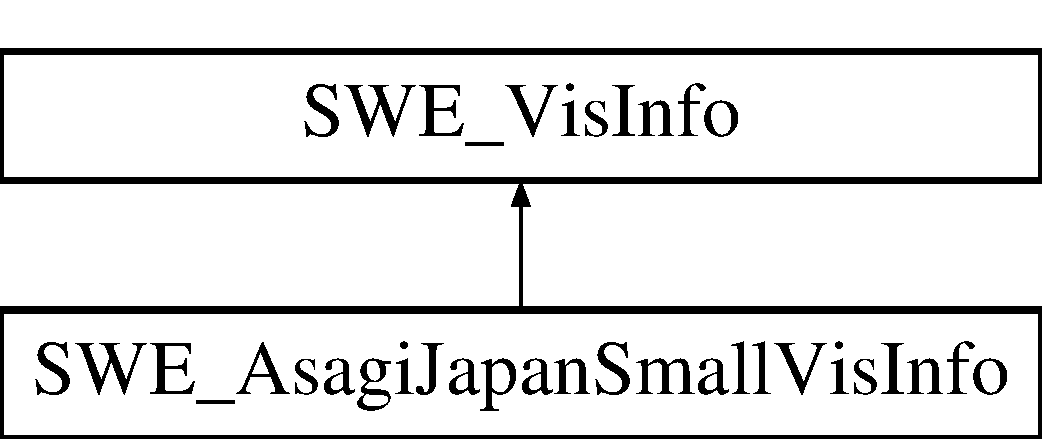
\includegraphics[height=2.000000cm]{classSWE__AsagiJapanSmallVisInfo}
\end{center}
\end{figure}
\subsection*{Public Member Functions}
\begin{DoxyCompactItemize}
\item 
virtual float {\bf water\-Vertical\-Scaling} ()
\item 
virtual float {\bf bathy\-Vertical\-Scaling} ()
\end{DoxyCompactItemize}


\subsection{Member Function Documentation}
\index{S\-W\-E\-\_\-\-Asagi\-Japan\-Small\-Vis\-Info@{S\-W\-E\-\_\-\-Asagi\-Japan\-Small\-Vis\-Info}!bathy\-Vertical\-Scaling@{bathy\-Vertical\-Scaling}}
\index{bathy\-Vertical\-Scaling@{bathy\-Vertical\-Scaling}!SWE_AsagiJapanSmallVisInfo@{S\-W\-E\-\_\-\-Asagi\-Japan\-Small\-Vis\-Info}}
\subsubsection[{bathy\-Vertical\-Scaling}]{\setlength{\rightskip}{0pt plus 5cm}virtual float S\-W\-E\-\_\-\-Asagi\-Japan\-Small\-Vis\-Info\-::bathy\-Vertical\-Scaling (
\begin{DoxyParamCaption}
{}
\end{DoxyParamCaption}
)\hspace{0.3cm}{\ttfamily [inline]}, {\ttfamily [virtual]}}\label{classSWE__AsagiJapanSmallVisInfo_ab25d85575460a76d88b90e2c927d49ac}
\begin{DoxyReturn}{Returns}
The vertical scaling factor for the bathymetry 
\end{DoxyReturn}


Reimplemented from {\bf S\-W\-E\-\_\-\-Vis\-Info} \doxyref{}{p.}{classSWE__VisInfo_a10ddd7a192e67c69832e695e48b26e91}.

\index{S\-W\-E\-\_\-\-Asagi\-Japan\-Small\-Vis\-Info@{S\-W\-E\-\_\-\-Asagi\-Japan\-Small\-Vis\-Info}!water\-Vertical\-Scaling@{water\-Vertical\-Scaling}}
\index{water\-Vertical\-Scaling@{water\-Vertical\-Scaling}!SWE_AsagiJapanSmallVisInfo@{S\-W\-E\-\_\-\-Asagi\-Japan\-Small\-Vis\-Info}}
\subsubsection[{water\-Vertical\-Scaling}]{\setlength{\rightskip}{0pt plus 5cm}virtual float S\-W\-E\-\_\-\-Asagi\-Japan\-Small\-Vis\-Info\-::water\-Vertical\-Scaling (
\begin{DoxyParamCaption}
{}
\end{DoxyParamCaption}
)\hspace{0.3cm}{\ttfamily [inline]}, {\ttfamily [virtual]}}\label{classSWE__AsagiJapanSmallVisInfo_a9c2092b5e02596e5ca2ba57c39d3b77e}
\begin{DoxyReturn}{Returns}
The vertical scaling factor of the water 
\end{DoxyReturn}


Reimplemented from {\bf S\-W\-E\-\_\-\-Vis\-Info} \doxyref{}{p.}{classSWE__VisInfo_a9552a55a7581b7835d415315e2c17f04}.



The documentation for this class was generated from the following file\-:\begin{DoxyCompactItemize}
\item 
src/scenarios/{\bf S\-W\-E\-\_\-\-Asagi\-Scenario\-\_\-vis.\-hh}\end{DoxyCompactItemize}

\section{S\-W\-E\-\_\-\-Asagi\-Scenario Class Reference}
\label{classSWE__AsagiScenario}\index{S\-W\-E\-\_\-\-Asagi\-Scenario@{S\-W\-E\-\_\-\-Asagi\-Scenario}}
Inheritance diagram for S\-W\-E\-\_\-\-Asagi\-Scenario\-:\begin{figure}[H]
\begin{center}
\leavevmode
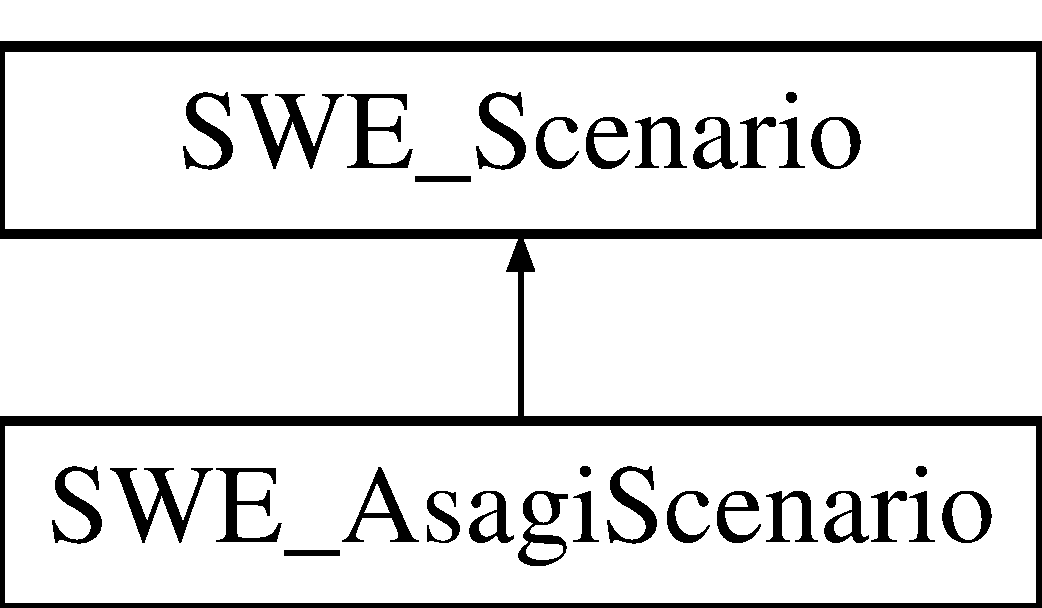
\includegraphics[height=2.000000cm]{classSWE__AsagiScenario}
\end{center}
\end{figure}
\subsection*{Public Member Functions}
\begin{DoxyCompactItemize}
\item 
{\bf S\-W\-E\-\_\-\-Asagi\-Scenario} (const std\-::string i\-\_\-bathymetry\-File, const std\-::string i\-\_\-displacement\-File, const float i\-\_\-duration, const float i\-\_\-simulation\-Area[4], const bool i\-\_\-dynamic\-Displacement=false)
\item 
void {\bfseries delete\-Grids} ()\label{classSWE__AsagiScenario_a48d6ba2326cbc06df693990cf41144e6}

\item 
float {\bf get\-Water\-Height} (float i\-\_\-position\-X, float i\-\_\-position\-Y)
\item 
float {\bf get\-Bathymetry} (const float i\-\_\-position\-X, const float i\-\_\-position\-Y)
\item 
float {\bf get\-Bathymetry\-And\-Dynamic\-Displacement} (const float i\-\_\-position\-X, const float i\-\_\-position\-Y, const float i\-\_\-time)
\item 
bool {\bf dynamic\-Displacement\-Available} (const float i\-\_\-time)
\item 
float {\bf end\-Simulation} ()
\item 
{\bf Boundary\-Type} {\bf get\-Boundary\-Type} ({\bf Boundary\-Edge} i\-\_\-edge)
\item 
float {\bf get\-Boundary\-Pos} ({\bf Boundary\-Edge} i\-\_\-edge)
\end{DoxyCompactItemize}


\subsection{Constructor \& Destructor Documentation}
\index{S\-W\-E\-\_\-\-Asagi\-Scenario@{S\-W\-E\-\_\-\-Asagi\-Scenario}!S\-W\-E\-\_\-\-Asagi\-Scenario@{S\-W\-E\-\_\-\-Asagi\-Scenario}}
\index{S\-W\-E\-\_\-\-Asagi\-Scenario@{S\-W\-E\-\_\-\-Asagi\-Scenario}!SWE_AsagiScenario@{S\-W\-E\-\_\-\-Asagi\-Scenario}}
\subsubsection[{S\-W\-E\-\_\-\-Asagi\-Scenario}]{\setlength{\rightskip}{0pt plus 5cm}S\-W\-E\-\_\-\-Asagi\-Scenario\-::\-S\-W\-E\-\_\-\-Asagi\-Scenario (
\begin{DoxyParamCaption}
\item[{const std\-::string}]{i\-\_\-bathymetry\-File, }
\item[{const std\-::string}]{i\-\_\-displacement\-File, }
\item[{const float}]{i\-\_\-duration, }
\item[{const float}]{i\-\_\-simulation\-Area[4], }
\item[{const bool}]{i\-\_\-dynamic\-Displacement = {\ttfamily false}}
\end{DoxyParamCaption}
)\hspace{0.3cm}{\ttfamily [inline]}}\label{classSWE__AsagiScenario_a9add0345b6793da297a44598451074e1}
Constructor of an Asagi Scenario, which initializes the corresponding Asagi grids.


\begin{DoxyParams}{Parameters}
{\em i\-\_\-origin\-X} & origin of the simulation area (x-\/direction) \\
\hline
{\em i\-\_\-origin\-Y} & origin of the simulation area (y-\/direction) \\
\hline
{\em i\-\_\-bathymetry\-File} & path to the net\-C\-D\-F-\/bathymetry file \\
\hline
{\em i\-\_\-displacement\-File} & path to the net\-C\-D\-F-\/displacement file \\
\hline
{\em i\-\_\-duration} & time the simulation runs (in seconds) \\
\hline
\end{DoxyParams}


\subsection{Member Function Documentation}
\index{S\-W\-E\-\_\-\-Asagi\-Scenario@{S\-W\-E\-\_\-\-Asagi\-Scenario}!dynamic\-Displacement\-Available@{dynamic\-Displacement\-Available}}
\index{dynamic\-Displacement\-Available@{dynamic\-Displacement\-Available}!SWE_AsagiScenario@{S\-W\-E\-\_\-\-Asagi\-Scenario}}
\subsubsection[{dynamic\-Displacement\-Available}]{\setlength{\rightskip}{0pt plus 5cm}bool S\-W\-E\-\_\-\-Asagi\-Scenario\-::dynamic\-Displacement\-Available (
\begin{DoxyParamCaption}
\item[{const float}]{i\-\_\-time}
\end{DoxyParamCaption}
)\hspace{0.3cm}{\ttfamily [inline]}}\label{classSWE__AsagiScenario_ada067ab5b456f445c66b9fe84c3a4ca5}
Check if there is an dynamic displacement is available for the corresponding time. 
\begin{DoxyParams}{Parameters}
{\em i\-\_\-time} & current simulation time \\
\hline
\end{DoxyParams}
\begin{DoxyReturn}{Returns}
true if there is data available, false else 
\end{DoxyReturn}
\index{S\-W\-E\-\_\-\-Asagi\-Scenario@{S\-W\-E\-\_\-\-Asagi\-Scenario}!end\-Simulation@{end\-Simulation}}
\index{end\-Simulation@{end\-Simulation}!SWE_AsagiScenario@{S\-W\-E\-\_\-\-Asagi\-Scenario}}
\subsubsection[{end\-Simulation}]{\setlength{\rightskip}{0pt plus 5cm}float S\-W\-E\-\_\-\-Asagi\-Scenario\-::end\-Simulation (
\begin{DoxyParamCaption}
{}
\end{DoxyParamCaption}
)\hspace{0.3cm}{\ttfamily [inline]}, {\ttfamily [virtual]}}\label{classSWE__AsagiScenario_a44449cbcfad023f60ae2af020576fe4b}
Get the number of seconds, the simulation should run. \begin{DoxyReturn}{Returns}
number of seconds, the simulation should run 
\end{DoxyReturn}


Reimplemented from {\bf S\-W\-E\-\_\-\-Scenario} \doxyref{}{p.}{classSWE__Scenario}.

\index{S\-W\-E\-\_\-\-Asagi\-Scenario@{S\-W\-E\-\_\-\-Asagi\-Scenario}!get\-Bathymetry@{get\-Bathymetry}}
\index{get\-Bathymetry@{get\-Bathymetry}!SWE_AsagiScenario@{S\-W\-E\-\_\-\-Asagi\-Scenario}}
\subsubsection[{get\-Bathymetry}]{\setlength{\rightskip}{0pt plus 5cm}float S\-W\-E\-\_\-\-Asagi\-Scenario\-::get\-Bathymetry (
\begin{DoxyParamCaption}
\item[{const float}]{i\-\_\-position\-X, }
\item[{const float}]{i\-\_\-position\-Y}
\end{DoxyParamCaption}
)\hspace{0.3cm}{\ttfamily [inline]}, {\ttfamily [virtual]}}\label{classSWE__AsagiScenario_a95456b79bd1f96120bd8efa73d927568}
Get the bathymetry including static displacement at a specific location


\begin{DoxyParams}{Parameters}
{\em i\-\_\-position\-X} & position relative to the origin of the displacement grid in x-\/direction \\
\hline
{\em i\-\_\-position\-Y} & position relative to the origin of the displacement grid in y-\/direction \\
\hline
\end{DoxyParams}
\begin{DoxyReturn}{Returns}
bathymetry (after the initial displacement (static displacement) 
\end{DoxyReturn}


Reimplemented from {\bf S\-W\-E\-\_\-\-Scenario} \doxyref{}{p.}{classSWE__Scenario}.

\index{S\-W\-E\-\_\-\-Asagi\-Scenario@{S\-W\-E\-\_\-\-Asagi\-Scenario}!get\-Bathymetry\-And\-Dynamic\-Displacement@{get\-Bathymetry\-And\-Dynamic\-Displacement}}
\index{get\-Bathymetry\-And\-Dynamic\-Displacement@{get\-Bathymetry\-And\-Dynamic\-Displacement}!SWE_AsagiScenario@{S\-W\-E\-\_\-\-Asagi\-Scenario}}
\subsubsection[{get\-Bathymetry\-And\-Dynamic\-Displacement}]{\setlength{\rightskip}{0pt plus 5cm}float S\-W\-E\-\_\-\-Asagi\-Scenario\-::get\-Bathymetry\-And\-Dynamic\-Displacement (
\begin{DoxyParamCaption}
\item[{const float}]{i\-\_\-position\-X, }
\item[{const float}]{i\-\_\-position\-Y, }
\item[{const float}]{i\-\_\-time}
\end{DoxyParamCaption}
)\hspace{0.3cm}{\ttfamily [inline]}}\label{classSWE__AsagiScenario_a462a4df01aec18b2e5af37f42e86cfde}
Get the bathymetry including dynamic displacement at a specific location


\begin{DoxyParams}{Parameters}
{\em i\-\_\-position\-X} & position relative to the origin of the displacement grid in x-\/direction \\
\hline
{\em i\-\_\-position\-Y} & position relative to the origin of the displacement grid in y-\/direction \\
\hline
{\em i\-\_\-time} & time relative to the origin of the dynamic displacement \\
\hline
\end{DoxyParams}
\begin{DoxyReturn}{Returns}
bathymetry (after the initial displacement (static displacement), after the specified amount of time (dynamic displacement)) 
\end{DoxyReturn}
\index{S\-W\-E\-\_\-\-Asagi\-Scenario@{S\-W\-E\-\_\-\-Asagi\-Scenario}!get\-Boundary\-Pos@{get\-Boundary\-Pos}}
\index{get\-Boundary\-Pos@{get\-Boundary\-Pos}!SWE_AsagiScenario@{S\-W\-E\-\_\-\-Asagi\-Scenario}}
\subsubsection[{get\-Boundary\-Pos}]{\setlength{\rightskip}{0pt plus 5cm}float S\-W\-E\-\_\-\-Asagi\-Scenario\-::get\-Boundary\-Pos (
\begin{DoxyParamCaption}
\item[{{\bf Boundary\-Edge}}]{i\-\_\-edge}
\end{DoxyParamCaption}
)\hspace{0.3cm}{\ttfamily [inline]}, {\ttfamily [virtual]}}\label{classSWE__AsagiScenario_a1f35638db4394f05fa2d0669634aa9ca}
Get the boundary positions


\begin{DoxyParams}{Parameters}
{\em i\-\_\-edge} & which edge \\
\hline
\end{DoxyParams}
\begin{DoxyReturn}{Returns}
value in the corresponding dimension 
\end{DoxyReturn}


Reimplemented from {\bf S\-W\-E\-\_\-\-Scenario} \doxyref{}{p.}{classSWE__Scenario}.

\index{S\-W\-E\-\_\-\-Asagi\-Scenario@{S\-W\-E\-\_\-\-Asagi\-Scenario}!get\-Boundary\-Type@{get\-Boundary\-Type}}
\index{get\-Boundary\-Type@{get\-Boundary\-Type}!SWE_AsagiScenario@{S\-W\-E\-\_\-\-Asagi\-Scenario}}
\subsubsection[{get\-Boundary\-Type}]{\setlength{\rightskip}{0pt plus 5cm}{\bf Boundary\-Type} S\-W\-E\-\_\-\-Asagi\-Scenario\-::get\-Boundary\-Type (
\begin{DoxyParamCaption}
\item[{{\bf Boundary\-Edge}}]{i\-\_\-edge}
\end{DoxyParamCaption}
)\hspace{0.3cm}{\ttfamily [inline]}, {\ttfamily [virtual]}}\label{classSWE__AsagiScenario_adf7992278300b2cb2475398245bad877}
Get the boundary types of the simulation 
\begin{DoxyParams}{Parameters}
{\em edge} & specific edge \\
\hline
\end{DoxyParams}
\begin{DoxyReturn}{Returns}
type of the edge 
\end{DoxyReturn}


Reimplemented from {\bf S\-W\-E\-\_\-\-Scenario} \doxyref{}{p.}{classSWE__Scenario}.

\index{S\-W\-E\-\_\-\-Asagi\-Scenario@{S\-W\-E\-\_\-\-Asagi\-Scenario}!get\-Water\-Height@{get\-Water\-Height}}
\index{get\-Water\-Height@{get\-Water\-Height}!SWE_AsagiScenario@{S\-W\-E\-\_\-\-Asagi\-Scenario}}
\subsubsection[{get\-Water\-Height}]{\setlength{\rightskip}{0pt plus 5cm}float S\-W\-E\-\_\-\-Asagi\-Scenario\-::get\-Water\-Height (
\begin{DoxyParamCaption}
\item[{float}]{i\-\_\-position\-X, }
\item[{float}]{i\-\_\-position\-Y}
\end{DoxyParamCaption}
)\hspace{0.3cm}{\ttfamily [inline]}, {\ttfamily [virtual]}}\label{classSWE__AsagiScenario_a3d2772883dc584cb1c8ffaafa4dafb8f}
Get the water height at a specific location (before the initial displacement).


\begin{DoxyParams}{Parameters}
{\em i\-\_\-position\-X} & position relative to the origin of the bathymetry grid in x-\/direction \\
\hline
{\em i\-\_\-position\-Y} & position relative to the origin of the bathymetry grid in y-\/direction \\
\hline
\end{DoxyParams}
\begin{DoxyReturn}{Returns}
water height (before the initial displacement) 
\end{DoxyReturn}


Reimplemented from {\bf S\-W\-E\-\_\-\-Scenario} \doxyref{}{p.}{classSWE__Scenario}.



The documentation for this class was generated from the following files\-:\begin{DoxyCompactItemize}
\item 
src/scenarios/{\bf S\-W\-E\-\_\-\-Asagi\-Scenario.\-hh}\item 
src/scenarios/{\bf S\-W\-E\-\_\-\-Asagi\-Scenario.\-cpp}\end{DoxyCompactItemize}

\section{S\-W\-E\-\_\-\-Bathymetry\-Dam\-Break\-Scenario Class Reference}
\label{classSWE__BathymetryDamBreakScenario}\index{S\-W\-E\-\_\-\-Bathymetry\-Dam\-Break\-Scenario@{S\-W\-E\-\_\-\-Bathymetry\-Dam\-Break\-Scenario}}


{\ttfamily \#include $<$S\-W\-E\-\_\-simple\-\_\-scenarios.\-hh$>$}

Inheritance diagram for S\-W\-E\-\_\-\-Bathymetry\-Dam\-Break\-Scenario\-:\begin{figure}[H]
\begin{center}
\leavevmode
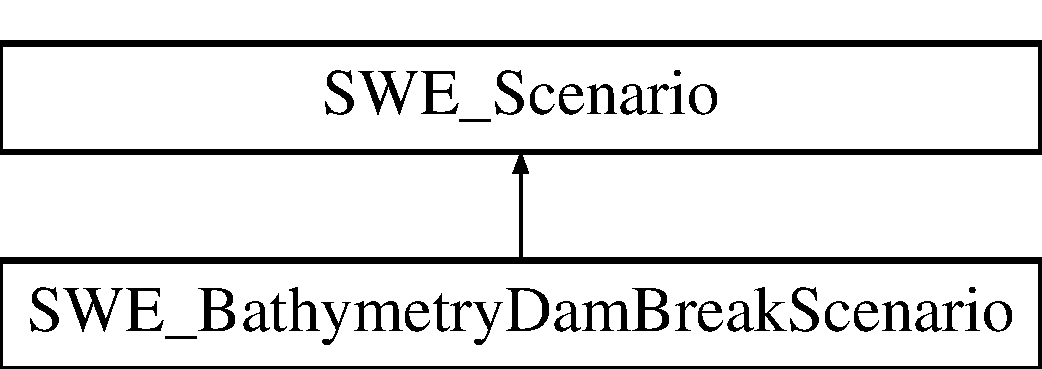
\includegraphics[height=2.000000cm]{classSWE__BathymetryDamBreakScenario}
\end{center}
\end{figure}
\subsection*{Public Member Functions}
\begin{DoxyCompactItemize}
\item 
float {\bfseries get\-Bathymetry} (float x, float y)\label{classSWE__BathymetryDamBreakScenario_abbc8b6d317163f21d2e9d46f67a6465f}

\item 
virtual float {\bfseries end\-Simulation} ()\label{classSWE__BathymetryDamBreakScenario_a29a5d3d82ad7092504b79a263c766feb}

\item 
virtual {\bf Boundary\-Type} {\bfseries get\-Boundary\-Type} ({\bf Boundary\-Edge} edge)\label{classSWE__BathymetryDamBreakScenario_ac7a07d56d659238c0dc099c6251e265b}

\item 
float {\bf get\-Boundary\-Pos} ({\bf Boundary\-Edge} i\-\_\-edge)
\item 
float {\bf get\-Water\-Height} (float i\-\_\-position\-X, float i\-\_\-position\-Y)
\end{DoxyCompactItemize}


\subsection{Detailed Description}
Scenario \char`\"{}\-Bathymetry Dam Break\char`\"{}\-: uniform water depth, but elevated bathymetry in the centre of the domain 

\subsection{Member Function Documentation}
\index{S\-W\-E\-\_\-\-Bathymetry\-Dam\-Break\-Scenario@{S\-W\-E\-\_\-\-Bathymetry\-Dam\-Break\-Scenario}!get\-Boundary\-Pos@{get\-Boundary\-Pos}}
\index{get\-Boundary\-Pos@{get\-Boundary\-Pos}!SWE_BathymetryDamBreakScenario@{S\-W\-E\-\_\-\-Bathymetry\-Dam\-Break\-Scenario}}
\subsubsection[{get\-Boundary\-Pos}]{\setlength{\rightskip}{0pt plus 5cm}float S\-W\-E\-\_\-\-Bathymetry\-Dam\-Break\-Scenario\-::get\-Boundary\-Pos (
\begin{DoxyParamCaption}
\item[{{\bf Boundary\-Edge}}]{i\-\_\-edge}
\end{DoxyParamCaption}
)\hspace{0.3cm}{\ttfamily [inline]}, {\ttfamily [virtual]}}\label{classSWE__BathymetryDamBreakScenario_aa861ba2d4d7e71509f78e1d4d4cb82c7}
Get the boundary positions


\begin{DoxyParams}{Parameters}
{\em i\-\_\-edge} & which edge \\
\hline
\end{DoxyParams}
\begin{DoxyReturn}{Returns}
value in the corresponding dimension 
\end{DoxyReturn}


Reimplemented from {\bf S\-W\-E\-\_\-\-Scenario} \doxyref{}{p.}{classSWE__Scenario}.

\index{S\-W\-E\-\_\-\-Bathymetry\-Dam\-Break\-Scenario@{S\-W\-E\-\_\-\-Bathymetry\-Dam\-Break\-Scenario}!get\-Water\-Height@{get\-Water\-Height}}
\index{get\-Water\-Height@{get\-Water\-Height}!SWE_BathymetryDamBreakScenario@{S\-W\-E\-\_\-\-Bathymetry\-Dam\-Break\-Scenario}}
\subsubsection[{get\-Water\-Height}]{\setlength{\rightskip}{0pt plus 5cm}float S\-W\-E\-\_\-\-Bathymetry\-Dam\-Break\-Scenario\-::get\-Water\-Height (
\begin{DoxyParamCaption}
\item[{float}]{i\-\_\-position\-X, }
\item[{float}]{i\-\_\-position\-Y}
\end{DoxyParamCaption}
)\hspace{0.3cm}{\ttfamily [inline]}, {\ttfamily [virtual]}}\label{classSWE__BathymetryDamBreakScenario_aa903538480526b092fff75160d7e225c}
Get the water height at a specific location.


\begin{DoxyParams}{Parameters}
{\em i\-\_\-position\-X} & position relative to the origin of the bathymetry grid in x-\/direction \\
\hline
{\em i\-\_\-position\-Y} & position relative to the origin of the bathymetry grid in y-\/direction \\
\hline
\end{DoxyParams}
\begin{DoxyReturn}{Returns}
water height (before the initial displacement) 
\end{DoxyReturn}


Reimplemented from {\bf S\-W\-E\-\_\-\-Scenario} \doxyref{}{p.}{classSWE__Scenario}.



The documentation for this class was generated from the following file\-:\begin{DoxyCompactItemize}
\item 
src/scenarios/{\bf S\-W\-E\-\_\-simple\-\_\-scenarios.\-hh}\end{DoxyCompactItemize}

\section{S\-W\-E\-\_\-\-Bathymetry\-Dam\-Break\-Vis\-Info Class Reference}
\label{classSWE__BathymetryDamBreakVisInfo}\index{S\-W\-E\-\_\-\-Bathymetry\-Dam\-Break\-Vis\-Info@{S\-W\-E\-\_\-\-Bathymetry\-Dam\-Break\-Vis\-Info}}


{\ttfamily \#include $<$S\-W\-E\-\_\-simple\-\_\-scenarios\-\_\-vis.\-hh$>$}

Inheritance diagram for S\-W\-E\-\_\-\-Bathymetry\-Dam\-Break\-Vis\-Info\-:\begin{figure}[H]
\begin{center}
\leavevmode
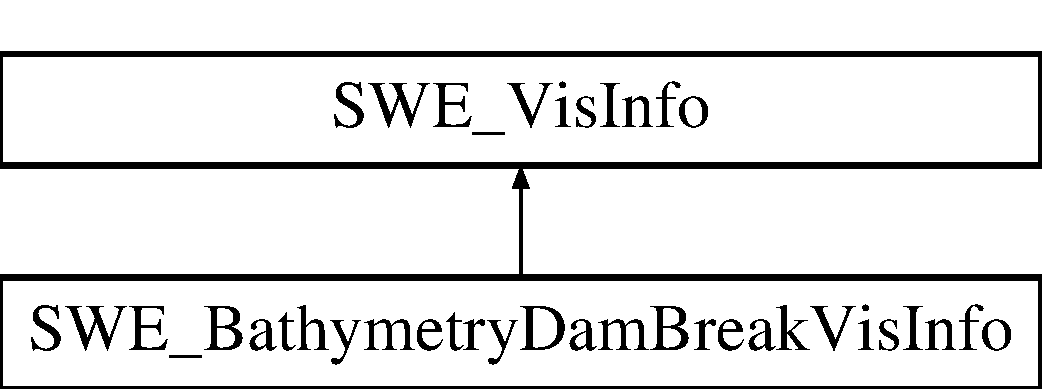
\includegraphics[height=2.000000cm]{classSWE__BathymetryDamBreakVisInfo}
\end{center}
\end{figure}
\subsection*{Public Member Functions}
\begin{DoxyCompactItemize}
\item 
float {\bf bathy\-Vertical\-Offset} ()
\end{DoxyCompactItemize}


\subsection{Detailed Description}
Vis\-Info \char`\"{}\-Bathymetry Dam Break\char`\"{}\-: uniform water depth, but elevated bathymetry in the center of the domain Set bathymetry offset hence it is visible in the screen 

\subsection{Member Function Documentation}
\index{S\-W\-E\-\_\-\-Bathymetry\-Dam\-Break\-Vis\-Info@{S\-W\-E\-\_\-\-Bathymetry\-Dam\-Break\-Vis\-Info}!bathy\-Vertical\-Offset@{bathy\-Vertical\-Offset}}
\index{bathy\-Vertical\-Offset@{bathy\-Vertical\-Offset}!SWE_BathymetryDamBreakVisInfo@{S\-W\-E\-\_\-\-Bathymetry\-Dam\-Break\-Vis\-Info}}
\subsubsection[{bathy\-Vertical\-Offset}]{\setlength{\rightskip}{0pt plus 5cm}float S\-W\-E\-\_\-\-Bathymetry\-Dam\-Break\-Vis\-Info\-::bathy\-Vertical\-Offset (
\begin{DoxyParamCaption}
{}
\end{DoxyParamCaption}
)\hspace{0.3cm}{\ttfamily [inline]}, {\ttfamily [virtual]}}\label{classSWE__BathymetryDamBreakVisInfo_aaecf007665b780a6066485ea0d2d2695}
\begin{DoxyReturn}{Returns}
The vertical offset for the bathymetry. Should be 0 for \char`\"{}real\char`\"{} scenarios (scenarios with dry areas) 
\end{DoxyReturn}


Reimplemented from {\bf S\-W\-E\-\_\-\-Vis\-Info} \doxyref{}{p.}{classSWE__VisInfo_a9c24e444c209f6f0c03a96950931e677}.



The documentation for this class was generated from the following file\-:\begin{DoxyCompactItemize}
\item 
src/scenarios/S\-W\-E\-\_\-simple\-\_\-scenarios\-\_\-vis.\-hh\end{DoxyCompactItemize}

\section{S\-W\-E\-\_\-\-Block Class Reference}
\label{classSWE__Block}\index{S\-W\-E\-\_\-\-Block@{S\-W\-E\-\_\-\-Block}}


{\ttfamily \#include $<$S\-W\-E\-\_\-\-Block.\-hh$>$}

Inheritance diagram for S\-W\-E\-\_\-\-Block\-:\begin{figure}[H]
\begin{center}
\leavevmode
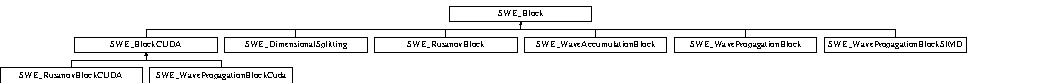
\includegraphics[height=1.111111cm]{classSWE__Block}
\end{center}
\end{figure}
\subsection*{Public Member Functions}
\begin{DoxyCompactItemize}
\item 
void {\bf init\-Scenario} (float \-\_\-offset\-X, float \-\_\-offset\-Y, {\bf S\-W\-E\-\_\-\-Scenario} \&i\-\_\-scenario, const bool i\-\_\-multiple\-Blocks=false)
\begin{DoxyCompactList}\small\item\em initialise unknowns to a specific scenario\-: \end{DoxyCompactList}\item 
void {\bf set\-Water\-Height} (float($\ast$\-\_\-h)(float, float))
\begin{DoxyCompactList}\small\item\em set the water height according to a given function \end{DoxyCompactList}\item 
void {\bf set\-Discharge} (float($\ast$\-\_\-u)(float, float), float($\ast$\-\_\-v)(float, float))
\begin{DoxyCompactList}\small\item\em set the momentum/discharge according to the provided functions \end{DoxyCompactList}\item 
void {\bf set\-Bathymetry} (float \-\_\-b)
\begin{DoxyCompactList}\small\item\em set the bathymetry to a uniform value \end{DoxyCompactList}\item 
void {\bf set\-Bathymetry} (float($\ast$\-\_\-b)(float, float))
\begin{DoxyCompactList}\small\item\em set the bathymetry according to a given function \end{DoxyCompactList}\item 
const {\bf Float2\-D} \& {\bf get\-Water\-Height} ()
\begin{DoxyCompactList}\small\item\em provides read access to the water height array \end{DoxyCompactList}\item 
const {\bf Float2\-D} \& {\bf get\-Discharge\-\_\-hu} ()
\begin{DoxyCompactList}\small\item\em provides read access to the momentum/discharge array (x-\/component) \end{DoxyCompactList}\item 
const {\bf Float2\-D} \& {\bf get\-Discharge\-\_\-hv} ()
\begin{DoxyCompactList}\small\item\em provides read access to the momentum/discharge array (y-\/component) \end{DoxyCompactList}\item 
const {\bf Float2\-D} \& {\bf get\-Bathymetry} ()
\begin{DoxyCompactList}\small\item\em provides read access to the bathymetry data \end{DoxyCompactList}\item 
void {\bf set\-Boundary\-Type} ({\bf Boundary\-Edge} edge, {\bf Boundary\-Type} boundtype, const {\bf S\-W\-E\-\_\-\-Block1\-D} $\ast$inflow=N\-U\-L\-L)
\begin{DoxyCompactList}\small\item\em set type of boundary condition for the specified boundary \end{DoxyCompactList}\item 
virtual {\bf S\-W\-E\-\_\-\-Block1\-D} $\ast$ {\bf register\-Copy\-Layer} ({\bf Boundary\-Edge} edge)
\begin{DoxyCompactList}\small\item\em return a pointer to proxy class to access the copy layer \end{DoxyCompactList}\item 
virtual {\bf S\-W\-E\-\_\-\-Block1\-D} $\ast$ {\bf grab\-Ghost\-Layer} ({\bf Boundary\-Edge} edge)
\begin{DoxyCompactList}\small\item\em \char`\"{}grab\char`\"{} the ghost layer in order to set these values externally \end{DoxyCompactList}\item 
void {\bf set\-Ghost\-Layer} ()
\begin{DoxyCompactList}\small\item\em set values in ghost layers \end{DoxyCompactList}\item 
float {\bf get\-Max\-Timestep} ()
\begin{DoxyCompactList}\small\item\em return maximum size of the time step to ensure stability of the method \end{DoxyCompactList}\item 
void {\bf compute\-Max\-Timestep} (const float i\-\_\-dry\-Tol=0.\-1, const float i\-\_\-cfl\-Number=0.\-4)
\item 
virtual void {\bf simulate\-Timestep} (float dt)
\begin{DoxyCompactList}\small\item\em execute a single time step (with fixed time step size) of the simulation \end{DoxyCompactList}\item 
virtual float {\bf simulate} (float t\-Start, float t\-End)
\item 
virtual void {\bf compute\-Numerical\-Fluxes} ()=0
\begin{DoxyCompactList}\small\item\em compute the numerical fluxes for each edge of the Cartesian grid \end{DoxyCompactList}\item 
virtual void {\bf update\-Unknowns} (float dt)=0
\begin{DoxyCompactList}\small\item\em compute the new values of the unknowns h, hu, and hv in all grid cells \end{DoxyCompactList}\item 
int {\bf get\-Nx} ()\label{classSWE__Block_aa27028fa4bc13bb2d9251b09e0fdfce6}

\begin{DoxyCompactList}\small\item\em returns \doxyref{nx}{p.}{classSWE__Block_a46ec0dc1157997bd255fb39924f1e2bb}, i.\-e. the grid size in x-\/direction \end{DoxyCompactList}\item 
int {\bf get\-Ny} ()\label{classSWE__Block_a4b65557b6f73ffb6454dad3dbf86e9ad}

\begin{DoxyCompactList}\small\item\em returns \doxyref{ny}{p.}{classSWE__Block_a3f139630d12423eb4bd7df3e45c7f5da}, i.\-e. the grid size in y-\/direction \end{DoxyCompactList}\end{DoxyCompactItemize}
\subsection*{Static Public Attributes}
\begin{DoxyCompactItemize}
\item 
static const float {\bf g} = 9.\-81f\label{classSWE__Block_a073ca743ff4077a7e456906be704958f}

\begin{DoxyCompactList}\small\item\em static variable that holds the gravity constant (g = 9.\-81 m/s$^\wedge$2)\-: \end{DoxyCompactList}\end{DoxyCompactItemize}
\subsection*{Protected Member Functions}
\begin{DoxyCompactItemize}
\item 
{\bf S\-W\-E\-\_\-\-Block} (int l\-\_\-nx, int l\-\_\-ny, float l\-\_\-dx, float l\-\_\-dy)
\item 
virtual {\bf $\sim$\-S\-W\-E\-\_\-\-Block} ()
\item 
void {\bf set\-Boundary\-Bathymetry} ()
\item 
virtual void {\bf synch\-After\-Write} ()
\item 
virtual void {\bf synch\-Water\-Height\-After\-Write} ()
\item 
virtual void {\bf synch\-Discharge\-After\-Write} ()
\item 
virtual void {\bf synch\-Bathymetry\-After\-Write} ()
\item 
virtual void {\bf synch\-Ghost\-Layer\-After\-Write} ()
\item 
virtual void {\bf synch\-Before\-Read} ()
\item 
virtual void {\bf synch\-Water\-Height\-Before\-Read} ()
\item 
virtual void {\bf synch\-Discharge\-Before\-Read} ()
\item 
virtual void {\bf synch\-Bathymetry\-Before\-Read} ()
\item 
virtual void {\bf synch\-Copy\-Layer\-Before\-Read} ()
\item 
virtual void {\bf set\-Boundary\-Conditions} ()
\begin{DoxyCompactList}\small\item\em set boundary conditions in ghost layers (set boundary conditions) \end{DoxyCompactList}\end{DoxyCompactItemize}
\subsection*{Protected Attributes}
\begin{DoxyCompactItemize}
\item 
int {\bf nx}\label{classSWE__Block_a46ec0dc1157997bd255fb39924f1e2bb}

\begin{DoxyCompactList}\small\item\em size of Cartesian arrays in x-\/direction \end{DoxyCompactList}\item 
int {\bf ny}\label{classSWE__Block_a3f139630d12423eb4bd7df3e45c7f5da}

\begin{DoxyCompactList}\small\item\em size of Cartesian arrays in y-\/direction \end{DoxyCompactList}\item 
float {\bf dx}\label{classSWE__Block_af2262b1cce6834d939c5a2315dae49b1}

\begin{DoxyCompactList}\small\item\em mesh size of the Cartesian grid in x-\/direction \end{DoxyCompactList}\item 
float {\bf dy}\label{classSWE__Block_a9feb988748d792bca0ca0508e43bd87f}

\begin{DoxyCompactList}\small\item\em mesh size of the Cartesian grid in y-\/direction \end{DoxyCompactList}\item 
{\bf Float2\-D} {\bf h}\label{classSWE__Block_a64a0f8f437f38b5f3b8ec5b4abdb864e}

\begin{DoxyCompactList}\small\item\em array that holds the water height for each element \end{DoxyCompactList}\item 
{\bf Float2\-D} {\bf hu}\label{classSWE__Block_aec2c1278fdb23f083216d8d397f26060}

\begin{DoxyCompactList}\small\item\em array that holds the x-\/component of the momentum for each element (water height h multiplied by velocity in x-\/direction) \end{DoxyCompactList}\item 
{\bf Float2\-D} {\bf hv}\label{classSWE__Block_a0897aa3c2d78749f209c95e08196d831}

\begin{DoxyCompactList}\small\item\em array that holds the y-\/component of the momentum for each element (water height h multiplied by velocity in y-\/direction) \end{DoxyCompactList}\item 
{\bf Float2\-D} {\bf b}\label{classSWE__Block_af7487209129f40b26ea171762754a261}

\begin{DoxyCompactList}\small\item\em array that holds the bathymetry data (sea floor elevation) for each element \end{DoxyCompactList}\item 
{\bf Boundary\-Type} {\bf boundary} [4]\label{classSWE__Block_a0e56d0cad169abd4f5de95d9f96c7a73}

\begin{DoxyCompactList}\small\item\em type of boundary conditions at L\-E\-F\-T, R\-I\-G\-H\-T, T\-O\-P, and B\-O\-T\-T\-O\-M boundary \end{DoxyCompactList}\item 
const {\bf S\-W\-E\-\_\-\-Block1\-D} $\ast$ {\bf neighbour} [4]\label{classSWE__Block_a5ea4ea4815af9eb66c51de9ad9b8d148}

\begin{DoxyCompactList}\small\item\em for C\-O\-N\-N\-E\-C\-T boundaries\-: pointer to connected neighbour block \end{DoxyCompactList}\item 
float {\bf max\-Timestep}
\begin{DoxyCompactList}\small\item\em maximum time step allowed to ensure stability of the method \end{DoxyCompactList}\item 
float {\bf offset\-X}\label{classSWE__Block_aa9e9b1fa797c133c4989e4c54f09b542}

\begin{DoxyCompactList}\small\item\em x-\/coordinate of the origin (left-\/bottom corner) of the Cartesian grid \end{DoxyCompactList}\item 
float {\bf offset\-Y}\label{classSWE__Block_aa05241101a66f0f0548eba6dbbaa1bbb}

\begin{DoxyCompactList}\small\item\em y-\/coordinate of the origin (left-\/bottom corner) of the Cartesian grid \end{DoxyCompactList}\end{DoxyCompactItemize}


\subsection{Detailed Description}
\doxyref{S\-W\-E\-\_\-\-Block}{p.}{classSWE__Block} is the main data structure to compute our shallow water model on a single Cartesian grid block\-: \doxyref{S\-W\-E\-\_\-\-Block}{p.}{classSWE__Block} is an abstract class (and interface) that should be extended by respective implementation classes.

\paragraph*{Cartesian Grid for Discretization\-:}

S\-W\-E\-\_\-\-Blocks uses a regular Cartesian grid of size \doxyref{nx}{p.}{classSWE__Block_a46ec0dc1157997bd255fb39924f1e2bb} by \doxyref{ny}{p.}{classSWE__Block_a3f139630d12423eb4bd7df3e45c7f5da}, where each grid cell carries three unknowns\-:
\begin{DoxyItemize}
\item the water level \doxyref{h}{p.}{classSWE__Block_a64a0f8f437f38b5f3b8ec5b4abdb864e}
\item the momentum components \doxyref{hu}{p.}{classSWE__Block_aec2c1278fdb23f083216d8d397f26060} and \doxyref{hv}{p.}{classSWE__Block_a0897aa3c2d78749f209c95e08196d831} (in x-\/ and y-\/ direction, resp.)
\item the bathymetry \doxyref{b}{p.}{classSWE__Block_af7487209129f40b26ea171762754a261}
\end{DoxyItemize}

Each of the components is stored as a 2\-D array, implemented as a \doxyref{Float2\-D}{p.}{classFloat2D} object, and are defined on grid indices [0,..,\doxyref{nx}{p.}{classSWE__Block_a46ec0dc1157997bd255fb39924f1e2bb}+1]$\ast$[0,..,\doxyref{ny}{p.}{classSWE__Block_a3f139630d12423eb4bd7df3e45c7f5da}+1]. The computational domain is indexed with [1,..,\doxyref{nx}{p.}{classSWE__Block_a46ec0dc1157997bd255fb39924f1e2bb}]$\ast$[1,..,\doxyref{ny}{p.}{classSWE__Block_a3f139630d12423eb4bd7df3e45c7f5da}].

The mesh sizes of the grid in x-\/ and y-\/direction are stored in static variables \doxyref{dx}{p.}{classSWE__Block_af2262b1cce6834d939c5a2315dae49b1} and \doxyref{dy}{p.}{classSWE__Block_a9feb988748d792bca0ca0508e43bd87f}. The position of the Cartesian grid in space is stored via the coordinates of the left-\/bottom corner of the grid, in the variables \doxyref{offset\-X}{p.}{classSWE__Block_aa9e9b1fa797c133c4989e4c54f09b542} and \doxyref{offset\-Y}{p.}{classSWE__Block_aa05241101a66f0f0548eba6dbbaa1bbb}.

\paragraph*{Ghost layers\-:}

To implement the behaviour of the fluid at boundaries and for using multiple block in serial and parallel settings, \doxyref{S\-W\-E\-\_\-\-Block}{p.}{classSWE__Block} adds an additional layer of so-\/called ghost cells to the Cartesian grid, as illustrated in the following figure. Cells in the ghost layer have indices 0 or \doxyref{nx}{p.}{classSWE__Block_a46ec0dc1157997bd255fb39924f1e2bb}+1 / \doxyref{ny}{p.}{classSWE__Block_a3f139630d12423eb4bd7df3e45c7f5da}+1.



\paragraph*{Memory Model\-:}

The variables \doxyref{h}{p.}{classSWE__Block_a64a0f8f437f38b5f3b8ec5b4abdb864e}, \doxyref{hu}{p.}{classSWE__Block_aec2c1278fdb23f083216d8d397f26060}, \doxyref{hv}{p.}{classSWE__Block_a0897aa3c2d78749f209c95e08196d831} for water height and momentum will typically be updated by classes derived from \doxyref{S\-W\-E\-\_\-\-Block}{p.}{classSWE__Block}. However, it is not assumed that such and updated will be performed in every time step. Instead, subclasses are welcome to update \doxyref{h}{p.}{classSWE__Block_a64a0f8f437f38b5f3b8ec5b4abdb864e}, \doxyref{hu}{p.}{classSWE__Block_aec2c1278fdb23f083216d8d397f26060}, and \doxyref{hv}{p.}{classSWE__Block_a0897aa3c2d78749f209c95e08196d831} in a lazy fashion, and keep data in faster memory (incl. local memory of acceleration hardware, such as G\-P\-G\-P\-Us), instead.

It is assumed that the bathymetry data \doxyref{b}{p.}{classSWE__Block_af7487209129f40b26ea171762754a261} is not changed during the algorithm (up to the exceptions mentioned in the following).

To force a synchronization of the respective data structures, the following methods are provided as part of \doxyref{S\-W\-E\-\_\-\-Block}{p.}{classSWE__Block}\-:
\begin{DoxyItemize}
\item \doxyref{synch\-After\-Write()}{p.}{classSWE__Block_ae914f9bf6d4ef8f974f9f005114985e7} to synchronize \doxyref{h}{p.}{classSWE__Block_a64a0f8f437f38b5f3b8ec5b4abdb864e}, \doxyref{hu}{p.}{classSWE__Block_aec2c1278fdb23f083216d8d397f26060}, \doxyref{hv}{p.}{classSWE__Block_a0897aa3c2d78749f209c95e08196d831}, and \doxyref{b}{p.}{classSWE__Block_af7487209129f40b26ea171762754a261} after an external update (reading a file, e.\-g.);
\item \doxyref{synch\-Water\-Height\-After\-Write()}{p.}{classSWE__Block_aa2924833e29a795d8c04fb79bfe794de}, \doxyref{synch\-Discharge\-After\-Write()}{p.}{classSWE__Block_a94c34030153178c9d94f3f14be174eaf}, \doxyref{synch\-Bathymetry\-After\-Write()}{p.}{classSWE__Block_a4bece8aa90f67e55c40b91aab900febb}\-: to synchronize only \doxyref{h}{p.}{classSWE__Block_a64a0f8f437f38b5f3b8ec5b4abdb864e} or momentum (\doxyref{hu}{p.}{classSWE__Block_aec2c1278fdb23f083216d8d397f26060} and \doxyref{hv}{p.}{classSWE__Block_a0897aa3c2d78749f209c95e08196d831}) or bathymetry \doxyref{b}{p.}{classSWE__Block_af7487209129f40b26ea171762754a261};
\item \doxyref{synch\-Ghost\-Layer\-After\-Write()}{p.}{classSWE__Block_a4657993ebdb5f0132b077e63790d0b2b} to synchronize only the ghost layers
\item \doxyref{synch\-Before\-Read()}{p.}{classSWE__Block_a23d936cb9a4367092e5b2515f81fe819} to synchronize \doxyref{h}{p.}{classSWE__Block_a64a0f8f437f38b5f3b8ec5b4abdb864e}, \doxyref{hu}{p.}{classSWE__Block_aec2c1278fdb23f083216d8d397f26060}, \doxyref{hv}{p.}{classSWE__Block_a0897aa3c2d78749f209c95e08196d831}, and \doxyref{b}{p.}{classSWE__Block_af7487209129f40b26ea171762754a261} before an output of the variables (writing a visualization file, e.\-g.)
\item \doxyref{synch\-Water\-Height\-Before\-Read()}{p.}{classSWE__Block_a07c85681ab29106c3b164db969899ace}, \doxyref{synch\-Discharge\-Before\-Read()}{p.}{classSWE__Block_a3773dcb194212fb8cb40ab8465575aa1}, \doxyref{synch\-Bathymetry\-Before\-Read()}{p.}{classSWE__Block_a7c8258c6949518ca44f4e9ce89d33b09}\-: as \doxyref{synch\-Before\-Read()}{p.}{classSWE__Block_a23d936cb9a4367092e5b2515f81fe819}, but only for the specified variables
\item \doxyref{synch\-Copy\-Layer\-Before\-Read()}{p.}{classSWE__Block_a13c90d5a6596336013c41e73c8795f83}\-: synchronizes the copy layer only (i.\-e., a layer that is to be replicated in a neighbouring \doxyref{S\-W\-E\-\_\-\-Block}{p.}{classSWE__Block}.
\end{DoxyItemize}

\paragraph*{Derived Classes}

As \doxyref{S\-W\-E\-\_\-\-Block}{p.}{classSWE__Block} just provides an abstract base class together with the most important data structures, the implementation of concrete models is the job of respective derived classes (see the class diagram at the top of this page). Similar, parallel implementations that are based on a specific parallel programming model (such as Open\-M\-P) or parallel architecture (such as G\-P\-U/\-C\-U\-D\-A) should form subclasses of their own. Please refer to the documentation of these classes for more details on the model and on the parallelisation approach. 

\subsection{Constructor \& Destructor Documentation}
\index{S\-W\-E\-\_\-\-Block@{S\-W\-E\-\_\-\-Block}!S\-W\-E\-\_\-\-Block@{S\-W\-E\-\_\-\-Block}}
\index{S\-W\-E\-\_\-\-Block@{S\-W\-E\-\_\-\-Block}!SWE_Block@{S\-W\-E\-\_\-\-Block}}
\subsubsection[{S\-W\-E\-\_\-\-Block}]{\setlength{\rightskip}{0pt plus 5cm}S\-W\-E\-\_\-\-Block\-::\-S\-W\-E\-\_\-\-Block (
\begin{DoxyParamCaption}
\item[{int}]{l\-\_\-nx, }
\item[{int}]{l\-\_\-ny, }
\item[{float}]{l\-\_\-dx, }
\item[{float}]{l\-\_\-dy}
\end{DoxyParamCaption}
)\hspace{0.3cm}{\ttfamily [protected]}}\label{classSWE__Block_a114ed3bb6a8a2c482e5f94f768543b82}
Constructor\-: allocate variables for simulation

unknowns h (water height), hu,hv (discharge in x-\/ and y-\/direction), and b (bathymetry) are defined on grid indices [0,..,nx+1]$\ast$[0,..,ny+1] -\/$>$ computational domain is [1,..,nx]$\ast$[1,..,ny] -\/$>$ plus ghost cell layer

The constructor is protected\-: no instances of \doxyref{S\-W\-E\-\_\-\-Block}{p.}{classSWE__Block} can be generated. \index{S\-W\-E\-\_\-\-Block@{S\-W\-E\-\_\-\-Block}!$\sim$\-S\-W\-E\-\_\-\-Block@{$\sim$\-S\-W\-E\-\_\-\-Block}}
\index{$\sim$\-S\-W\-E\-\_\-\-Block@{$\sim$\-S\-W\-E\-\_\-\-Block}!SWE_Block@{S\-W\-E\-\_\-\-Block}}
\subsubsection[{$\sim$\-S\-W\-E\-\_\-\-Block}]{\setlength{\rightskip}{0pt plus 5cm}S\-W\-E\-\_\-\-Block\-::$\sim$\-S\-W\-E\-\_\-\-Block (
\begin{DoxyParamCaption}
{}
\end{DoxyParamCaption}
)\hspace{0.3cm}{\ttfamily [protected]}, {\ttfamily [virtual]}}\label{classSWE__Block_a2ddff1c284663ba514985a3574def1b0}
Destructor\-: de-\/allocate all variables 

\subsection{Member Function Documentation}
\index{S\-W\-E\-\_\-\-Block@{S\-W\-E\-\_\-\-Block}!compute\-Max\-Timestep@{compute\-Max\-Timestep}}
\index{compute\-Max\-Timestep@{compute\-Max\-Timestep}!SWE_Block@{S\-W\-E\-\_\-\-Block}}
\subsubsection[{compute\-Max\-Timestep}]{\setlength{\rightskip}{0pt plus 5cm}void S\-W\-E\-\_\-\-Block\-::compute\-Max\-Timestep (
\begin{DoxyParamCaption}
\item[{const float}]{i\-\_\-dry\-Tol = {\ttfamily 0.1}, }
\item[{const float}]{i\-\_\-cfl\-Number = {\ttfamily 0.4}}
\end{DoxyParamCaption}
)}\label{classSWE__Block_acf2ff6617cbc0d3d837f0e618039cfe2}
Compute the largest allowed time step for the current grid block (reference implementation) depending on the current values of variables h, hu, and hv, and store this time step size in member variable max\-Timestep.


\begin{DoxyParams}{Parameters}
{\em i\-\_\-dry\-Tol} & dry tolerance (dry cells do not affect the time step). \\
\hline
{\em i\-\_\-cfl\-Number} & C\-F\-L number of the used method. \\
\hline
\end{DoxyParams}
\index{S\-W\-E\-\_\-\-Block@{S\-W\-E\-\_\-\-Block}!compute\-Numerical\-Fluxes@{compute\-Numerical\-Fluxes}}
\index{compute\-Numerical\-Fluxes@{compute\-Numerical\-Fluxes}!SWE_Block@{S\-W\-E\-\_\-\-Block}}
\subsubsection[{compute\-Numerical\-Fluxes}]{\setlength{\rightskip}{0pt plus 5cm}virtual void S\-W\-E\-\_\-\-Block\-::compute\-Numerical\-Fluxes (
\begin{DoxyParamCaption}
{}
\end{DoxyParamCaption}
)\hspace{0.3cm}{\ttfamily [pure virtual]}}\label{classSWE__Block_a94dcf2c6ae31731e4586e45628b0c00e}


compute the numerical fluxes for each edge of the Cartesian grid 

The computation of fluxes strongly depends on the chosen numerical method. Hence, this purely virtual function has to be implemented in the respective derived classes. 

Implemented in {\bf S\-W\-E\-\_\-\-Dimensional\-Splitting} \doxyref{}{p.}{classSWE__DimensionalSplitting_a84759f8fbbbfe1e46613375515826f0f}, {\bf S\-W\-E\-\_\-\-Wave\-Propagation\-Block\-S\-I\-M\-D} \doxyref{}{p.}{classSWE__WavePropagationBlockSIMD_a4aa15050ec1db113f54fff06539a900f}, {\bf S\-W\-E\-\_\-\-Wave\-Propagation\-Block} \doxyref{}{p.}{classSWE__WavePropagationBlock_a5f6335a38fb3cf38623326959f06baf4}, {\bf S\-W\-E\-\_\-\-Wave\-Propagation\-Block\-Cuda} \doxyref{}{p.}{classSWE__WavePropagationBlockCuda_a8a89bf61b9fc4433652f400ca8e564ed}, {\bf S\-W\-E\-\_\-\-Wave\-Accumulation\-Block} \doxyref{}{p.}{classSWE__WaveAccumulationBlock_acac0b73f22b256bc91a58ff8d0831e5d}, {\bf S\-W\-E\-\_\-\-Rusanov\-Block} \doxyref{}{p.}{classSWE__RusanovBlock_a78cdefa510cd2d88ca4e213f75b9b10b}, and {\bf S\-W\-E\-\_\-\-Rusanov\-Block\-C\-U\-D\-A} \doxyref{}{p.}{classSWE__RusanovBlockCUDA_a64fa005a8f69f49ac7894dffcec39787}.

\index{S\-W\-E\-\_\-\-Block@{S\-W\-E\-\_\-\-Block}!get\-Bathymetry@{get\-Bathymetry}}
\index{get\-Bathymetry@{get\-Bathymetry}!SWE_Block@{S\-W\-E\-\_\-\-Block}}
\subsubsection[{get\-Bathymetry}]{\setlength{\rightskip}{0pt plus 5cm}const {\bf Float2\-D} \& S\-W\-E\-\_\-\-Block\-::get\-Bathymetry (
\begin{DoxyParamCaption}
{}
\end{DoxyParamCaption}
)}\label{classSWE__Block_a98e2c99a335d11d09a1489d6873b5615}


provides read access to the bathymetry data 

return reference to bathymetry unknown b \index{S\-W\-E\-\_\-\-Block@{S\-W\-E\-\_\-\-Block}!get\-Discharge\-\_\-hu@{get\-Discharge\-\_\-hu}}
\index{get\-Discharge\-\_\-hu@{get\-Discharge\-\_\-hu}!SWE_Block@{S\-W\-E\-\_\-\-Block}}
\subsubsection[{get\-Discharge\-\_\-hu}]{\setlength{\rightskip}{0pt plus 5cm}const {\bf Float2\-D} \& S\-W\-E\-\_\-\-Block\-::get\-Discharge\-\_\-hu (
\begin{DoxyParamCaption}
{}
\end{DoxyParamCaption}
)}\label{classSWE__Block_ae5e766626a1e3fee89625610e2c67f1f}


provides read access to the momentum/discharge array (x-\/component) 

return reference to discharge unknown hu \index{S\-W\-E\-\_\-\-Block@{S\-W\-E\-\_\-\-Block}!get\-Discharge\-\_\-hv@{get\-Discharge\-\_\-hv}}
\index{get\-Discharge\-\_\-hv@{get\-Discharge\-\_\-hv}!SWE_Block@{S\-W\-E\-\_\-\-Block}}
\subsubsection[{get\-Discharge\-\_\-hv}]{\setlength{\rightskip}{0pt plus 5cm}const {\bf Float2\-D} \& S\-W\-E\-\_\-\-Block\-::get\-Discharge\-\_\-hv (
\begin{DoxyParamCaption}
{}
\end{DoxyParamCaption}
)}\label{classSWE__Block_aece9e8dc3f9b8ab27420e537c76daf7c}


provides read access to the momentum/discharge array (y-\/component) 

return reference to discharge unknown hv \index{S\-W\-E\-\_\-\-Block@{S\-W\-E\-\_\-\-Block}!get\-Max\-Timestep@{get\-Max\-Timestep}}
\index{get\-Max\-Timestep@{get\-Max\-Timestep}!SWE_Block@{S\-W\-E\-\_\-\-Block}}
\subsubsection[{get\-Max\-Timestep}]{\setlength{\rightskip}{0pt plus 5cm}float S\-W\-E\-\_\-\-Block\-::get\-Max\-Timestep (
\begin{DoxyParamCaption}
{}
\end{DoxyParamCaption}
)\hspace{0.3cm}{\ttfamily [inline]}}\label{classSWE__Block_a74da1eb712e639e47b5b848081b2afad}


return maximum size of the time step to ensure stability of the method 

\begin{DoxyReturn}{Returns}
current value of the member variable \doxyref{max\-Timestep}{p.}{classSWE__Block_a05cbc9b40e0483bf73dbc2bdeae7dee3} 
\end{DoxyReturn}
\index{S\-W\-E\-\_\-\-Block@{S\-W\-E\-\_\-\-Block}!get\-Water\-Height@{get\-Water\-Height}}
\index{get\-Water\-Height@{get\-Water\-Height}!SWE_Block@{S\-W\-E\-\_\-\-Block}}
\subsubsection[{get\-Water\-Height}]{\setlength{\rightskip}{0pt plus 5cm}const {\bf Float2\-D} \& S\-W\-E\-\_\-\-Block\-::get\-Water\-Height (
\begin{DoxyParamCaption}
{}
\end{DoxyParamCaption}
)}\label{classSWE__Block_ab1aea4294403c194180c3dc107339fd7}


provides read access to the water height array 

Restores values for h, v, and u from file data 
\begin{DoxyParams}{Parameters}
{\em \-\_\-b} & array holding b-\/values in sequence return reference to water height unknown h \\
\hline
\end{DoxyParams}
\index{S\-W\-E\-\_\-\-Block@{S\-W\-E\-\_\-\-Block}!grab\-Ghost\-Layer@{grab\-Ghost\-Layer}}
\index{grab\-Ghost\-Layer@{grab\-Ghost\-Layer}!SWE_Block@{S\-W\-E\-\_\-\-Block}}
\subsubsection[{grab\-Ghost\-Layer}]{\setlength{\rightskip}{0pt plus 5cm}{\bf S\-W\-E\-\_\-\-Block1\-D} $\ast$ S\-W\-E\-\_\-\-Block\-::grab\-Ghost\-Layer (
\begin{DoxyParamCaption}
\item[{{\bf Boundary\-Edge}}]{edge}
\end{DoxyParamCaption}
)\hspace{0.3cm}{\ttfamily [virtual]}}\label{classSWE__Block_a9a96c59444645e237d098803009158a3}


\char`\"{}grab\char`\"{} the ghost layer in order to set these values externally 

\char`\"{}grab\char`\"{} the ghost layer at the specific boundary in order to set boundary values in this ghost layer externally. The boundary conditions at the respective ghost layer is set to P\-A\-S\-S\-I\-V\-E, such that the grabbing program component is responsible to provide correct values in the ghost layer, for example by receiving data from a remote copy layer via M\-P\-I communication. 
\begin{DoxyParams}{Parameters}
{\em specified} & edge \\
\hline
\end{DoxyParams}
\begin{DoxyReturn}{Returns}
a \doxyref{S\-W\-E\-\_\-\-Block1\-D}{p.}{structSWE__Block1D} object that contains row variables h, hu, and hv 
\end{DoxyReturn}


Reimplemented in {\bf S\-W\-E\-\_\-\-Block\-C\-U\-D\-A} \doxyref{}{p.}{classSWE__BlockCUDA_a266fd1b60d27be35103b089da72f1e6e}.

\index{S\-W\-E\-\_\-\-Block@{S\-W\-E\-\_\-\-Block}!init\-Scenario@{init\-Scenario}}
\index{init\-Scenario@{init\-Scenario}!SWE_Block@{S\-W\-E\-\_\-\-Block}}
\subsubsection[{init\-Scenario}]{\setlength{\rightskip}{0pt plus 5cm}void S\-W\-E\-\_\-\-Block\-::init\-Scenario (
\begin{DoxyParamCaption}
\item[{float}]{\-\_\-offset\-X, }
\item[{float}]{\-\_\-offset\-Y, }
\item[{{\bf S\-W\-E\-\_\-\-Scenario} \&}]{i\-\_\-scenario, }
\item[{const bool}]{i\-\_\-multiple\-Blocks = {\ttfamily false}}
\end{DoxyParamCaption}
)}\label{classSWE__Block_a46b715c584468a5daa975ec1eb1ab947}


initialise unknowns to a specific scenario\-: 

Initializes the unknowns and bathymetry in all grid cells according to the given \doxyref{S\-W\-E\-\_\-\-Scenario}{p.}{classSWE__Scenario}.

In the case of multiple S\-W\-E\-\_\-\-Blocks at this point, it is not clear how the boundary conditions should be set. This is because an isolated \doxyref{S\-W\-E\-\_\-\-Block}{p.}{classSWE__Block} doesn't have any in information about the grid. Therefore the calling routine, which has the information about multiple blocks, has to take care about setting the right boundary conditions.


\begin{DoxyParams}{Parameters}
{\em i\-\_\-scenario} & scenario, which is used during the setup. \\
\hline
{\em i\-\_\-multiple\-Blocks} & are the multiple S\-W\-E\-\_\-blocks? \\
\hline
\end{DoxyParams}
\index{S\-W\-E\-\_\-\-Block@{S\-W\-E\-\_\-\-Block}!register\-Copy\-Layer@{register\-Copy\-Layer}}
\index{register\-Copy\-Layer@{register\-Copy\-Layer}!SWE_Block@{S\-W\-E\-\_\-\-Block}}
\subsubsection[{register\-Copy\-Layer}]{\setlength{\rightskip}{0pt plus 5cm}{\bf S\-W\-E\-\_\-\-Block1\-D} $\ast$ S\-W\-E\-\_\-\-Block\-::register\-Copy\-Layer (
\begin{DoxyParamCaption}
\item[{{\bf Boundary\-Edge}}]{edge}
\end{DoxyParamCaption}
)\hspace{0.3cm}{\ttfamily [virtual]}}\label{classSWE__Block_a827ee5c61dc9c1b472ac8b4e1c19956a}


return a pointer to proxy class to access the copy layer 

register the row or column layer next to a boundary as a \char`\"{}copy layer\char`\"{}, from which values will be copied into the ghost layer or a neighbour; \begin{DoxyReturn}{Returns}
a \doxyref{S\-W\-E\-\_\-\-Block1\-D}{p.}{structSWE__Block1D} object that contains row variables h, hu, and hv 
\end{DoxyReturn}


Reimplemented in {\bf S\-W\-E\-\_\-\-Block\-C\-U\-D\-A} \doxyref{}{p.}{classSWE__BlockCUDA_a16660ec1c396be1fd1ace44aaa265d04}.

\index{S\-W\-E\-\_\-\-Block@{S\-W\-E\-\_\-\-Block}!set\-Bathymetry@{set\-Bathymetry}}
\index{set\-Bathymetry@{set\-Bathymetry}!SWE_Block@{S\-W\-E\-\_\-\-Block}}
\subsubsection[{set\-Bathymetry}]{\setlength{\rightskip}{0pt plus 5cm}void S\-W\-E\-\_\-\-Block\-::set\-Bathymetry (
\begin{DoxyParamCaption}
\item[{float}]{\-\_\-b}
\end{DoxyParamCaption}
)}\label{classSWE__Block_af2ab34b138a14f2c295849f3b2acc5f3}


set the bathymetry to a uniform value 

set Bathymetry b in all grid cells (incl. ghost/boundary layers) to a uniform value bathymetry source terms are re-\/computed \index{S\-W\-E\-\_\-\-Block@{S\-W\-E\-\_\-\-Block}!set\-Bathymetry@{set\-Bathymetry}}
\index{set\-Bathymetry@{set\-Bathymetry}!SWE_Block@{S\-W\-E\-\_\-\-Block}}
\subsubsection[{set\-Bathymetry}]{\setlength{\rightskip}{0pt plus 5cm}void S\-W\-E\-\_\-\-Block\-::set\-Bathymetry (
\begin{DoxyParamCaption}
\item[{float($\ast$)(float, float)}]{\-\_\-b}
\end{DoxyParamCaption}
)}\label{classSWE__Block_ad4214fcfd102a4c167d274ad87d9dd90}


set the bathymetry according to a given function 

set Bathymetry b in all grid cells (incl. ghost/boundary layers) using the specified bathymetry function; bathymetry source terms are re-\/computed \index{S\-W\-E\-\_\-\-Block@{S\-W\-E\-\_\-\-Block}!set\-Boundary\-Bathymetry@{set\-Boundary\-Bathymetry}}
\index{set\-Boundary\-Bathymetry@{set\-Boundary\-Bathymetry}!SWE_Block@{S\-W\-E\-\_\-\-Block}}
\subsubsection[{set\-Boundary\-Bathymetry}]{\setlength{\rightskip}{0pt plus 5cm}void S\-W\-E\-\_\-\-Block\-::set\-Boundary\-Bathymetry (
\begin{DoxyParamCaption}
{}
\end{DoxyParamCaption}
)\hspace{0.3cm}{\ttfamily [protected]}}\label{classSWE__Block_a6beb68dacde9c8479647c25c6a5cbcf5}
Sets the bathymetry on O\-U\-T\-F\-L\-O\-W or W\-A\-L\-L boundaries. Should be called very time a boundary is changed to a O\-U\-T\-F\-L\-O\-W or W\-A\-L\-L boundary {\bfseries or} the bathymetry changes. \index{S\-W\-E\-\_\-\-Block@{S\-W\-E\-\_\-\-Block}!set\-Boundary\-Conditions@{set\-Boundary\-Conditions}}
\index{set\-Boundary\-Conditions@{set\-Boundary\-Conditions}!SWE_Block@{S\-W\-E\-\_\-\-Block}}
\subsubsection[{set\-Boundary\-Conditions}]{\setlength{\rightskip}{0pt plus 5cm}void S\-W\-E\-\_\-\-Block\-::set\-Boundary\-Conditions (
\begin{DoxyParamCaption}
{}
\end{DoxyParamCaption}
)\hspace{0.3cm}{\ttfamily [protected]}, {\ttfamily [virtual]}}\label{classSWE__Block_a379807f0bf932b40aeb42065633fce60}


set boundary conditions in ghost layers (set boundary conditions) 

set the values of all ghost cells depending on the specifed boundary conditions
\begin{DoxyItemize}
\item set boundary conditions for typs W\-A\-L\-L and O\-U\-T\-F\-L\-O\-W
\item derived classes need to transfer ghost layers 
\end{DoxyItemize}

Reimplemented in {\bf S\-W\-E\-\_\-\-Block\-C\-U\-D\-A} \doxyref{}{p.}{classSWE__BlockCUDA_a01d0db0b1c5e7b0fbb1bb886382ba3ce}.

\index{S\-W\-E\-\_\-\-Block@{S\-W\-E\-\_\-\-Block}!set\-Boundary\-Type@{set\-Boundary\-Type}}
\index{set\-Boundary\-Type@{set\-Boundary\-Type}!SWE_Block@{S\-W\-E\-\_\-\-Block}}
\subsubsection[{set\-Boundary\-Type}]{\setlength{\rightskip}{0pt plus 5cm}void S\-W\-E\-\_\-\-Block\-::set\-Boundary\-Type (
\begin{DoxyParamCaption}
\item[{{\bf Boundary\-Edge}}]{edge, }
\item[{{\bf Boundary\-Type}}]{boundtype, }
\item[{const {\bf S\-W\-E\-\_\-\-Block1\-D} $\ast$}]{i\-\_\-inflow = {\ttfamily NULL}}
\end{DoxyParamCaption}
)}\label{classSWE__Block_aa220b93e43b10f56c72a44d7363645c1}


set type of boundary condition for the specified boundary 

Set the boundary type for specific block boundary.


\begin{DoxyParams}{Parameters}
{\em i\-\_\-edge} & location of the edge relative to the S\-W\-E\-\_\-block. \\
\hline
{\em i\-\_\-boundary\-Type} & type of the boundary condition. \\
\hline
{\em i\-\_\-inflow} & pointer to an \doxyref{S\-W\-E\-\_\-\-Block1\-D}{p.}{structSWE__Block1D}, which specifies the inflow (should be N\-U\-L\-L for W\-A\-L\-L or O\-U\-T\-F\-L\-O\-W boundary) \\
\hline
\end{DoxyParams}
\index{S\-W\-E\-\_\-\-Block@{S\-W\-E\-\_\-\-Block}!set\-Discharge@{set\-Discharge}}
\index{set\-Discharge@{set\-Discharge}!SWE_Block@{S\-W\-E\-\_\-\-Block}}
\subsubsection[{set\-Discharge}]{\setlength{\rightskip}{0pt plus 5cm}void S\-W\-E\-\_\-\-Block\-::set\-Discharge (
\begin{DoxyParamCaption}
\item[{float($\ast$)(float, float)}]{\-\_\-u, }
\item[{float($\ast$)(float, float)}]{\-\_\-v}
\end{DoxyParamCaption}
)}\label{classSWE__Block_a245332c325fd0ff6a7e9c2d3d9454970}


set the momentum/discharge according to the provided functions 

set discharge in all interior grid cells (i.\-e. except ghost layer) to values specified by parameter functions Note\-: unknowns hu and hv represent momentum, while parameters u and v are velocities! \index{S\-W\-E\-\_\-\-Block@{S\-W\-E\-\_\-\-Block}!set\-Ghost\-Layer@{set\-Ghost\-Layer}}
\index{set\-Ghost\-Layer@{set\-Ghost\-Layer}!SWE_Block@{S\-W\-E\-\_\-\-Block}}
\subsubsection[{set\-Ghost\-Layer}]{\setlength{\rightskip}{0pt plus 5cm}void S\-W\-E\-\_\-\-Block\-::set\-Ghost\-Layer (
\begin{DoxyParamCaption}
{}
\end{DoxyParamCaption}
)}\label{classSWE__Block_afd17334abee3145e27cc3c9b7b935da2}


set values in ghost layers 

set the values of all ghost cells depending on the specifed boundary conditions; if the ghost layer replicates the variables of a remote \doxyref{S\-W\-E\-\_\-\-Block}{p.}{classSWE__Block}, the values are copied \index{S\-W\-E\-\_\-\-Block@{S\-W\-E\-\_\-\-Block}!set\-Water\-Height@{set\-Water\-Height}}
\index{set\-Water\-Height@{set\-Water\-Height}!SWE_Block@{S\-W\-E\-\_\-\-Block}}
\subsubsection[{set\-Water\-Height}]{\setlength{\rightskip}{0pt plus 5cm}void S\-W\-E\-\_\-\-Block\-::set\-Water\-Height (
\begin{DoxyParamCaption}
\item[{float($\ast$)(float, float)}]{\-\_\-h}
\end{DoxyParamCaption}
)}\label{classSWE__Block_a6481ce1c80a219fbefefdcbd13ed3688}


set the water height according to a given function 

set water height h in all interior grid cells (i.\-e. except ghost layer) to values specified by parameter function \-\_\-h \index{S\-W\-E\-\_\-\-Block@{S\-W\-E\-\_\-\-Block}!simulate@{simulate}}
\index{simulate@{simulate}!SWE_Block@{S\-W\-E\-\_\-\-Block}}
\subsubsection[{simulate}]{\setlength{\rightskip}{0pt plus 5cm}float S\-W\-E\-\_\-\-Block\-::simulate (
\begin{DoxyParamCaption}
\item[{float}]{i\-\_\-t\-Start, }
\item[{float}]{i\-\_\-t\-End}
\end{DoxyParamCaption}
)\hspace{0.3cm}{\ttfamily [virtual]}}\label{classSWE__Block_a69784e2be2d09035fb2af9d306768f07}
perform the simulation starting with simulation time t\-Start, until simulation time t\-End is reached

simulate implements the main simulation loop between two checkpoints; Note\-: this implementation can only be used, if you only use a single \doxyref{S\-W\-E\-\_\-\-Block}{p.}{classSWE__Block} and only apply simple boundary conditions! In particular, \doxyref{S\-W\-E\-\_\-\-Block\-::simulate}{p.}{classSWE__Block_a69784e2be2d09035fb2af9d306768f07} can not trigger calls to exchange values of copy and ghost layers between blocks! 
\begin{DoxyParams}{Parameters}
{\em t\-Start} & time where the simulation is started \\
\hline
{\em t\-End} & time of the next checkpoint \\
\hline
\end{DoxyParams}
\begin{DoxyReturn}{Returns}
actual end time reached 
\end{DoxyReturn}


Reimplemented in {\bf S\-W\-E\-\_\-\-Wave\-Propagation\-Block\-S\-I\-M\-D} \doxyref{}{p.}{classSWE__WavePropagationBlockSIMD_a6c54dbcd43a77b46bae4de36b8d16af7}, {\bf S\-W\-E\-\_\-\-Wave\-Propagation\-Block\-Cuda} \doxyref{}{p.}{classSWE__WavePropagationBlockCuda_aa7cb155a2c8a76171fa39daff2b30ce3}, {\bf S\-W\-E\-\_\-\-Rusanov\-Block\-C\-U\-D\-A} \doxyref{}{p.}{classSWE__RusanovBlockCUDA_a42c63cf7d3c5609768aa28263393efb6}, and {\bf S\-W\-E\-\_\-\-Rusanov\-Block} \doxyref{}{p.}{classSWE__RusanovBlock_a645322106b3e5b6f0cca077611ad2159}.

\index{S\-W\-E\-\_\-\-Block@{S\-W\-E\-\_\-\-Block}!simulate\-Timestep@{simulate\-Timestep}}
\index{simulate\-Timestep@{simulate\-Timestep}!SWE_Block@{S\-W\-E\-\_\-\-Block}}
\subsubsection[{simulate\-Timestep}]{\setlength{\rightskip}{0pt plus 5cm}void S\-W\-E\-\_\-\-Block\-::simulate\-Timestep (
\begin{DoxyParamCaption}
\item[{float}]{dt}
\end{DoxyParamCaption}
)\hspace{0.3cm}{\ttfamily [virtual]}}\label{classSWE__Block_add6908e1ceb261a0a1f3ebc262cc5f11}


execute a single time step (with fixed time step size) of the simulation 

Executes a single timestep with fixed time step size
\begin{DoxyItemize}
\item compute net updates for every edge
\item update cell values with the net updates
\end{DoxyItemize}


\begin{DoxyParams}{Parameters}
{\em dt} & time step width of the update \\
\hline
\end{DoxyParams}


Reimplemented in {\bf S\-W\-E\-\_\-\-Wave\-Propagation\-Block\-S\-I\-M\-D} \doxyref{}{p.}{classSWE__WavePropagationBlockSIMD_a99c288632c402eaf7dff76f03624872a}, {\bf S\-W\-E\-\_\-\-Wave\-Propagation\-Block\-Cuda} \doxyref{}{p.}{classSWE__WavePropagationBlockCuda_a1e79efd0b3f90e793add52fd5155410a}, {\bf S\-W\-E\-\_\-\-Rusanov\-Block\-C\-U\-D\-A} \doxyref{}{p.}{classSWE__RusanovBlockCUDA_aa039b202a505cf31ab16e8c74dc4153b}, and {\bf S\-W\-E\-\_\-\-Rusanov\-Block} \doxyref{}{p.}{classSWE__RusanovBlock_ada062db4f54700011d50378b0045830a}.

\index{S\-W\-E\-\_\-\-Block@{S\-W\-E\-\_\-\-Block}!synch\-After\-Write@{synch\-After\-Write}}
\index{synch\-After\-Write@{synch\-After\-Write}!SWE_Block@{S\-W\-E\-\_\-\-Block}}
\subsubsection[{synch\-After\-Write}]{\setlength{\rightskip}{0pt plus 5cm}void S\-W\-E\-\_\-\-Block\-::synch\-After\-Write (
\begin{DoxyParamCaption}
{}
\end{DoxyParamCaption}
)\hspace{0.3cm}{\ttfamily [protected]}, {\ttfamily [virtual]}}\label{classSWE__Block_ae914f9bf6d4ef8f974f9f005114985e7}
Update all temporary and non-\/local (for heterogeneous computing) variables after an external update of the main variables h, hu, hv, and b. 

Reimplemented in {\bf S\-W\-E\-\_\-\-Block\-C\-U\-D\-A} \doxyref{}{p.}{classSWE__BlockCUDA_ac0df7dd281db264b3ce06d8ae6d4c004}.

\index{S\-W\-E\-\_\-\-Block@{S\-W\-E\-\_\-\-Block}!synch\-Bathymetry\-After\-Write@{synch\-Bathymetry\-After\-Write}}
\index{synch\-Bathymetry\-After\-Write@{synch\-Bathymetry\-After\-Write}!SWE_Block@{S\-W\-E\-\_\-\-Block}}
\subsubsection[{synch\-Bathymetry\-After\-Write}]{\setlength{\rightskip}{0pt plus 5cm}void S\-W\-E\-\_\-\-Block\-::synch\-Bathymetry\-After\-Write (
\begin{DoxyParamCaption}
{}
\end{DoxyParamCaption}
)\hspace{0.3cm}{\ttfamily [protected]}, {\ttfamily [virtual]}}\label{classSWE__Block_a4bece8aa90f67e55c40b91aab900febb}
Update temporary and non-\/local (for heterogeneous computing) variables after an external update of the bathymetry b 

Reimplemented in {\bf S\-W\-E\-\_\-\-Block\-C\-U\-D\-A} \doxyref{}{p.}{classSWE__BlockCUDA_afb390e026d984f3a33727addcd9c6f00}.

\index{S\-W\-E\-\_\-\-Block@{S\-W\-E\-\_\-\-Block}!synch\-Bathymetry\-Before\-Read@{synch\-Bathymetry\-Before\-Read}}
\index{synch\-Bathymetry\-Before\-Read@{synch\-Bathymetry\-Before\-Read}!SWE_Block@{S\-W\-E\-\_\-\-Block}}
\subsubsection[{synch\-Bathymetry\-Before\-Read}]{\setlength{\rightskip}{0pt plus 5cm}void S\-W\-E\-\_\-\-Block\-::synch\-Bathymetry\-Before\-Read (
\begin{DoxyParamCaption}
{}
\end{DoxyParamCaption}
)\hspace{0.3cm}{\ttfamily [protected]}, {\ttfamily [virtual]}}\label{classSWE__Block_a7c8258c6949518ca44f4e9ce89d33b09}
Update temporary and non-\/local (for heterogeneous computing) variables before an external access to the bathymetry b 

Reimplemented in {\bf S\-W\-E\-\_\-\-Block\-C\-U\-D\-A} \doxyref{}{p.}{classSWE__BlockCUDA_a8c5ee2bb3afadf44451a434dbd1cba6e}.

\index{S\-W\-E\-\_\-\-Block@{S\-W\-E\-\_\-\-Block}!synch\-Before\-Read@{synch\-Before\-Read}}
\index{synch\-Before\-Read@{synch\-Before\-Read}!SWE_Block@{S\-W\-E\-\_\-\-Block}}
\subsubsection[{synch\-Before\-Read}]{\setlength{\rightskip}{0pt plus 5cm}void S\-W\-E\-\_\-\-Block\-::synch\-Before\-Read (
\begin{DoxyParamCaption}
{}
\end{DoxyParamCaption}
)\hspace{0.3cm}{\ttfamily [protected]}, {\ttfamily [virtual]}}\label{classSWE__Block_a23d936cb9a4367092e5b2515f81fe819}
Update all temporary and non-\/local (for heterogeneous computing) variables before an external access to the main variables h, hu, hv, and b. 

Reimplemented in {\bf S\-W\-E\-\_\-\-Block\-C\-U\-D\-A} \doxyref{}{p.}{classSWE__BlockCUDA_aa81487c41270362dfcaafdd911ec358d}.

\index{S\-W\-E\-\_\-\-Block@{S\-W\-E\-\_\-\-Block}!synch\-Copy\-Layer\-Before\-Read@{synch\-Copy\-Layer\-Before\-Read}}
\index{synch\-Copy\-Layer\-Before\-Read@{synch\-Copy\-Layer\-Before\-Read}!SWE_Block@{S\-W\-E\-\_\-\-Block}}
\subsubsection[{synch\-Copy\-Layer\-Before\-Read}]{\setlength{\rightskip}{0pt plus 5cm}void S\-W\-E\-\_\-\-Block\-::synch\-Copy\-Layer\-Before\-Read (
\begin{DoxyParamCaption}
{}
\end{DoxyParamCaption}
)\hspace{0.3cm}{\ttfamily [protected]}, {\ttfamily [virtual]}}\label{classSWE__Block_a13c90d5a6596336013c41e73c8795f83}
Update (for heterogeneous computing) variables in copy layers before an external access to the unknowns 

Reimplemented in {\bf S\-W\-E\-\_\-\-Block\-C\-U\-D\-A} \doxyref{}{p.}{classSWE__BlockCUDA_af14ae578fc5afa8d85ca94c827c1d310}.

\index{S\-W\-E\-\_\-\-Block@{S\-W\-E\-\_\-\-Block}!synch\-Discharge\-After\-Write@{synch\-Discharge\-After\-Write}}
\index{synch\-Discharge\-After\-Write@{synch\-Discharge\-After\-Write}!SWE_Block@{S\-W\-E\-\_\-\-Block}}
\subsubsection[{synch\-Discharge\-After\-Write}]{\setlength{\rightskip}{0pt plus 5cm}void S\-W\-E\-\_\-\-Block\-::synch\-Discharge\-After\-Write (
\begin{DoxyParamCaption}
{}
\end{DoxyParamCaption}
)\hspace{0.3cm}{\ttfamily [protected]}, {\ttfamily [virtual]}}\label{classSWE__Block_a94c34030153178c9d94f3f14be174eaf}
Update temporary and non-\/local (for heterogeneous computing) variables after an external update of the discharge variables hu and hv 

Reimplemented in {\bf S\-W\-E\-\_\-\-Block\-C\-U\-D\-A} \doxyref{}{p.}{classSWE__BlockCUDA_a01274791529721345e4611e40942a006}.

\index{S\-W\-E\-\_\-\-Block@{S\-W\-E\-\_\-\-Block}!synch\-Discharge\-Before\-Read@{synch\-Discharge\-Before\-Read}}
\index{synch\-Discharge\-Before\-Read@{synch\-Discharge\-Before\-Read}!SWE_Block@{S\-W\-E\-\_\-\-Block}}
\subsubsection[{synch\-Discharge\-Before\-Read}]{\setlength{\rightskip}{0pt plus 5cm}void S\-W\-E\-\_\-\-Block\-::synch\-Discharge\-Before\-Read (
\begin{DoxyParamCaption}
{}
\end{DoxyParamCaption}
)\hspace{0.3cm}{\ttfamily [protected]}, {\ttfamily [virtual]}}\label{classSWE__Block_a3773dcb194212fb8cb40ab8465575aa1}
Update temporary and non-\/local (for heterogeneous computing) variables before an external access to the discharge variables hu and hv 

Reimplemented in {\bf S\-W\-E\-\_\-\-Block\-C\-U\-D\-A} \doxyref{}{p.}{classSWE__BlockCUDA_ab244fbc1c2a926806a489c67d8644cf2}.

\index{S\-W\-E\-\_\-\-Block@{S\-W\-E\-\_\-\-Block}!synch\-Ghost\-Layer\-After\-Write@{synch\-Ghost\-Layer\-After\-Write}}
\index{synch\-Ghost\-Layer\-After\-Write@{synch\-Ghost\-Layer\-After\-Write}!SWE_Block@{S\-W\-E\-\_\-\-Block}}
\subsubsection[{synch\-Ghost\-Layer\-After\-Write}]{\setlength{\rightskip}{0pt plus 5cm}void S\-W\-E\-\_\-\-Block\-::synch\-Ghost\-Layer\-After\-Write (
\begin{DoxyParamCaption}
{}
\end{DoxyParamCaption}
)\hspace{0.3cm}{\ttfamily [protected]}, {\ttfamily [virtual]}}\label{classSWE__Block_a4657993ebdb5f0132b077e63790d0b2b}
Update the ghost layers (only for C\-O\-N\-N\-E\-C\-T and P\-A\-S\-S\-I\-V\-E boundary conditions) after an external update of the main variables h, hu, hv, and b in the ghost layer. 

Reimplemented in {\bf S\-W\-E\-\_\-\-Block\-C\-U\-D\-A} \doxyref{}{p.}{classSWE__BlockCUDA_ac2f31de45c6aee8ca5a54e8bec4d64c7}.

\index{S\-W\-E\-\_\-\-Block@{S\-W\-E\-\_\-\-Block}!synch\-Water\-Height\-After\-Write@{synch\-Water\-Height\-After\-Write}}
\index{synch\-Water\-Height\-After\-Write@{synch\-Water\-Height\-After\-Write}!SWE_Block@{S\-W\-E\-\_\-\-Block}}
\subsubsection[{synch\-Water\-Height\-After\-Write}]{\setlength{\rightskip}{0pt plus 5cm}void S\-W\-E\-\_\-\-Block\-::synch\-Water\-Height\-After\-Write (
\begin{DoxyParamCaption}
{}
\end{DoxyParamCaption}
)\hspace{0.3cm}{\ttfamily [protected]}, {\ttfamily [virtual]}}\label{classSWE__Block_aa2924833e29a795d8c04fb79bfe794de}
Update temporary and non-\/local (for heterogeneous computing) variables after an external update of the water height h 

Reimplemented in {\bf S\-W\-E\-\_\-\-Block\-C\-U\-D\-A} \doxyref{}{p.}{classSWE__BlockCUDA_af15f84ed38f89f62b33a7b56daec84c8}.

\index{S\-W\-E\-\_\-\-Block@{S\-W\-E\-\_\-\-Block}!synch\-Water\-Height\-Before\-Read@{synch\-Water\-Height\-Before\-Read}}
\index{synch\-Water\-Height\-Before\-Read@{synch\-Water\-Height\-Before\-Read}!SWE_Block@{S\-W\-E\-\_\-\-Block}}
\subsubsection[{synch\-Water\-Height\-Before\-Read}]{\setlength{\rightskip}{0pt plus 5cm}void S\-W\-E\-\_\-\-Block\-::synch\-Water\-Height\-Before\-Read (
\begin{DoxyParamCaption}
{}
\end{DoxyParamCaption}
)\hspace{0.3cm}{\ttfamily [protected]}, {\ttfamily [virtual]}}\label{classSWE__Block_a07c85681ab29106c3b164db969899ace}
Update temporary and non-\/local (for heterogeneous computing) variables before an external access to the water height h 

Reimplemented in {\bf S\-W\-E\-\_\-\-Block\-C\-U\-D\-A} \doxyref{}{p.}{classSWE__BlockCUDA_abb2738cc673335b52d1cac2e0d8cfc53}.

\index{S\-W\-E\-\_\-\-Block@{S\-W\-E\-\_\-\-Block}!update\-Unknowns@{update\-Unknowns}}
\index{update\-Unknowns@{update\-Unknowns}!SWE_Block@{S\-W\-E\-\_\-\-Block}}
\subsubsection[{update\-Unknowns}]{\setlength{\rightskip}{0pt plus 5cm}virtual void S\-W\-E\-\_\-\-Block\-::update\-Unknowns (
\begin{DoxyParamCaption}
\item[{float}]{dt}
\end{DoxyParamCaption}
)\hspace{0.3cm}{\ttfamily [pure virtual]}}\label{classSWE__Block_ab2b4b659f23d5d45413dece8d2da3298}


compute the new values of the unknowns h, hu, and hv in all grid cells 

based on the numerical fluxes (computed by compute\-Numerical\-Fluxes) and the specified time step size dt, an Euler time step is executed. As the computational fluxes will depend on the numerical method, this purely virtual function has to be implemented separately for each specific numerical model (and parallelisation approach). 
\begin{DoxyParams}{Parameters}
{\em dt} & size of the time step \\
\hline
\end{DoxyParams}


Implemented in {\bf S\-W\-E\-\_\-\-Dimensional\-Splitting} \doxyref{}{p.}{classSWE__DimensionalSplitting_af74b527ff9ca7727442db92d2e438531}, {\bf S\-W\-E\-\_\-\-Wave\-Propagation\-Block\-S\-I\-M\-D} \doxyref{}{p.}{classSWE__WavePropagationBlockSIMD_a2596238868efd3cdd453d9ac2de15997}, {\bf S\-W\-E\-\_\-\-Wave\-Propagation\-Block} \doxyref{}{p.}{classSWE__WavePropagationBlock_a1b1422472a36602b34180e4ed27f6d8c}, {\bf S\-W\-E\-\_\-\-Wave\-Propagation\-Block\-Cuda} \doxyref{}{p.}{classSWE__WavePropagationBlockCuda_a4163045a47a73515841e754ca3859fc5}, {\bf S\-W\-E\-\_\-\-Wave\-Accumulation\-Block} \doxyref{}{p.}{classSWE__WaveAccumulationBlock_a67b78723e81aec6e661b3710e6c41b43}, {\bf S\-W\-E\-\_\-\-Rusanov\-Block} \doxyref{}{p.}{classSWE__RusanovBlock_a2980aa21030ba8fc607001ad817d7454}, and {\bf S\-W\-E\-\_\-\-Rusanov\-Block\-C\-U\-D\-A} \doxyref{}{p.}{classSWE__RusanovBlockCUDA_a037264d8f044fd4d323420562c82a218}.



\subsection{Member Data Documentation}
\index{S\-W\-E\-\_\-\-Block@{S\-W\-E\-\_\-\-Block}!max\-Timestep@{max\-Timestep}}
\index{max\-Timestep@{max\-Timestep}!SWE_Block@{S\-W\-E\-\_\-\-Block}}
\subsubsection[{max\-Timestep}]{\setlength{\rightskip}{0pt plus 5cm}float S\-W\-E\-\_\-\-Block\-::max\-Timestep\hspace{0.3cm}{\ttfamily [protected]}}\label{classSWE__Block_a05cbc9b40e0483bf73dbc2bdeae7dee3}


maximum time step allowed to ensure stability of the method 

max\-Timestep can be updated as part of the methods compute\-Numerical\-Fluxes and update\-Unknowns (depending on the numerical method) 

The documentation for this class was generated from the following files\-:\begin{DoxyCompactItemize}
\item 
src/blocks/{\bf S\-W\-E\-\_\-\-Block.\-hh}\item 
src/blocks/{\bf S\-W\-E\-\_\-\-Block.\-cpp}\end{DoxyCompactItemize}

\section{S\-W\-E\-\_\-\-Block1\-D Struct Reference}
\label{structSWE__Block1D}\index{S\-W\-E\-\_\-\-Block1\-D@{S\-W\-E\-\_\-\-Block1\-D}}


{\ttfamily \#include $<$S\-W\-E\-\_\-\-Block.\-hh$>$}

\subsection*{Public Member Functions}
\begin{DoxyCompactItemize}
\item 
{\bfseries S\-W\-E\-\_\-\-Block1\-D} (const {\bf Float1\-D} \&\-\_\-h, const {\bf Float1\-D} \&\-\_\-hu, const {\bf Float1\-D} \&\-\_\-hv)\label{structSWE__Block1D_a29516674bf63c42f9fd99995c09f4d55}

\item 
{\bfseries S\-W\-E\-\_\-\-Block1\-D} (float $\ast$\-\_\-h, float $\ast$\-\_\-hu, float $\ast$\-\_\-hv, int \-\_\-size, int \-\_\-stride=1)\label{structSWE__Block1D_a9b23e09458246ba4212a1fbfc52206cc}

\end{DoxyCompactItemize}
\subsection*{Public Attributes}
\begin{DoxyCompactItemize}
\item 
{\bf Float1\-D} {\bfseries h}\label{structSWE__Block1D_a7bea1da024ec63e77753fe32880fc5d2}

\item 
{\bf Float1\-D} {\bfseries hu}\label{structSWE__Block1D_a8662233fe9b86ead9ef2a419103271e5}

\item 
{\bf Float1\-D} {\bfseries hv}\label{structSWE__Block1D_aa261d9fcdb400d7da349f41dfa6d5b4f}

\end{DoxyCompactItemize}


\subsection{Detailed Description}
\doxyref{S\-W\-E\-\_\-\-Block1\-D}{p.}{structSWE__Block1D} is a simple struct that can represent a single line or row of \doxyref{S\-W\-E\-\_\-\-Block}{p.}{classSWE__Block} unknowns (using the \doxyref{Float1\-D}{p.}{classFloat1D} proxy class). It is intended to unify the implementation of inflow and periodic boundary conditions, as well as the ghost/copy-\/layer connection between several \doxyref{S\-W\-E\-\_\-\-Block}{p.}{classSWE__Block} grids. 

The documentation for this struct was generated from the following file\-:\begin{DoxyCompactItemize}
\item 
src/blocks/{\bf S\-W\-E\-\_\-\-Block.\-hh}\end{DoxyCompactItemize}

\section{S\-W\-E\-\_\-\-Block\-C\-U\-D\-A Class Reference}
\label{classSWE__BlockCUDA}\index{S\-W\-E\-\_\-\-Block\-C\-U\-D\-A@{S\-W\-E\-\_\-\-Block\-C\-U\-D\-A}}


{\ttfamily \#include $<$S\-W\-E\-\_\-\-Block\-C\-U\-D\-A.\-hh$>$}

Inheritance diagram for S\-W\-E\-\_\-\-Block\-C\-U\-D\-A\-:\begin{figure}[H]
\begin{center}
\leavevmode
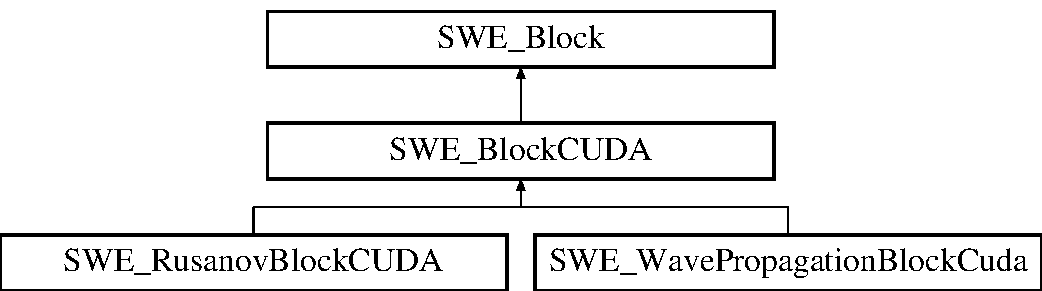
\includegraphics[height=3.000000cm]{classSWE__BlockCUDA}
\end{center}
\end{figure}
\subsection*{Public Member Functions}
\begin{DoxyCompactItemize}
\item 
{\bfseries S\-W\-E\-\_\-\-Block\-C\-U\-D\-A} (int l\-\_\-nx, int l\-\_\-ny, float l\-\_\-dx, float l\-\_\-dy)\label{classSWE__BlockCUDA_a7e4f5f08cf6179d17e7ff64cb2f182d8}

\item 
virtual {\bf S\-W\-E\-\_\-\-Block1\-D} $\ast$ {\bf register\-Copy\-Layer} ({\bf Boundary\-Edge} edge)
\begin{DoxyCompactList}\small\item\em return a pointer to proxy class to access the copy layer \end{DoxyCompactList}\item 
virtual {\bf S\-W\-E\-\_\-\-Block1\-D} $\ast$ {\bf grab\-Ghost\-Layer} ({\bf Boundary\-Edge} edge)
\begin{DoxyCompactList}\small\item\em \char`\"{}grab\char`\"{} the ghost layer in order to set these values externally \end{DoxyCompactList}\item 
const float $\ast$ {\bf get\-C\-U\-D\-A\-\_\-water\-Height} ()
\item 
const float $\ast$ {\bf get\-C\-U\-D\-A\-\_\-bathymetry} ()
\end{DoxyCompactItemize}
\subsection*{Static Public Member Functions}
\begin{DoxyCompactItemize}
\item 
static void {\bfseries print\-Device\-Information} ()\label{classSWE__BlockCUDA_ac64dc736eb4be4346d00f0947c948f85}

\item 
static void {\bf init} (int i\-\_\-cuda\-Device=0)
\item 
static void {\bf finalize} ()
\end{DoxyCompactItemize}
\subsection*{Protected Member Functions}
\begin{DoxyCompactItemize}
\item 
virtual void {\bf synch\-After\-Write} ()
\item 
virtual void {\bf synch\-Water\-Height\-After\-Write} ()
\item 
virtual void {\bf synch\-Discharge\-After\-Write} ()
\item 
virtual void {\bf synch\-Bathymetry\-After\-Write} ()
\item 
virtual void {\bf synch\-Ghost\-Layer\-After\-Write} ()
\item 
virtual void {\bf synch\-Before\-Read} ()
\item 
virtual void {\bf synch\-Water\-Height\-Before\-Read} ()
\item 
virtual void {\bf synch\-Discharge\-Before\-Read} ()
\item 
virtual void {\bf synch\-Bathymetry\-Before\-Read} ()
\item 
virtual void {\bf synch\-Copy\-Layer\-Before\-Read} ()
\item 
virtual void {\bf set\-Boundary\-Conditions} ()
\begin{DoxyCompactList}\small\item\em set boundary conditions in ghost layers (set boundary conditions) \end{DoxyCompactList}\end{DoxyCompactItemize}
\subsection*{Protected Attributes}
\begin{DoxyCompactItemize}
\item 
float $\ast$ {\bfseries hd}\label{classSWE__BlockCUDA_a9c6a44214a75a9f5d4f8bb3806eaaf71}

\item 
float $\ast$ {\bfseries hud}\label{classSWE__BlockCUDA_a2fb123601bbf091876dcccc351157c67}

\item 
float $\ast$ {\bfseries hvd}\label{classSWE__BlockCUDA_a795fe87f7abfa7e6511232e03a808705}

\item 
float $\ast$ {\bfseries bd}\label{classSWE__BlockCUDA_ae08ee1752690e828a9e0470a3c55fb39}

\end{DoxyCompactItemize}
\subsection*{Additional Inherited Members}


\subsection{Detailed Description}
\doxyref{S\-W\-E\-\_\-\-Block\-C\-U\-D\-A}{p.}{classSWE__BlockCUDA} extends the base class \doxyref{S\-W\-E\-\_\-\-Block}{p.}{classSWE__Block} towards a base class for a C\-U\-D\-A implementation of the shallow water equations. It adds the respective variables in G\-P\-U memory, and provides methods for data transfer between main and G\-P\-U memory. 

\subsection{Member Function Documentation}
\index{S\-W\-E\-\_\-\-Block\-C\-U\-D\-A@{S\-W\-E\-\_\-\-Block\-C\-U\-D\-A}!finalize@{finalize}}
\index{finalize@{finalize}!SWE_BlockCUDA@{S\-W\-E\-\_\-\-Block\-C\-U\-D\-A}}
\subsubsection[{finalize}]{\setlength{\rightskip}{0pt plus 5cm}static void S\-W\-E\-\_\-\-Block\-C\-U\-D\-A\-::finalize (
\begin{DoxyParamCaption}
{}
\end{DoxyParamCaption}
)\hspace{0.3cm}{\ttfamily [static]}}\label{classSWE__BlockCUDA_abcb4cf7eb9fe2cf0dbf517fa96f3c2c3}
Cleans up the cuda device \index{S\-W\-E\-\_\-\-Block\-C\-U\-D\-A@{S\-W\-E\-\_\-\-Block\-C\-U\-D\-A}!get\-C\-U\-D\-A\-\_\-bathymetry@{get\-C\-U\-D\-A\-\_\-bathymetry}}
\index{get\-C\-U\-D\-A\-\_\-bathymetry@{get\-C\-U\-D\-A\-\_\-bathymetry}!SWE_BlockCUDA@{S\-W\-E\-\_\-\-Block\-C\-U\-D\-A}}
\subsubsection[{get\-C\-U\-D\-A\-\_\-bathymetry}]{\setlength{\rightskip}{0pt plus 5cm}const float$\ast$ S\-W\-E\-\_\-\-Block\-C\-U\-D\-A\-::get\-C\-U\-D\-A\-\_\-bathymetry (
\begin{DoxyParamCaption}
{}
\end{DoxyParamCaption}
)\hspace{0.3cm}{\ttfamily [inline]}}\label{classSWE__BlockCUDA_ad8bf853a1319ed215010dc05c78d33e6}
\begin{DoxyReturn}{Returns}
pointer to the array \#hb (bathymetry) in device memory 
\end{DoxyReturn}
\index{S\-W\-E\-\_\-\-Block\-C\-U\-D\-A@{S\-W\-E\-\_\-\-Block\-C\-U\-D\-A}!get\-C\-U\-D\-A\-\_\-water\-Height@{get\-C\-U\-D\-A\-\_\-water\-Height}}
\index{get\-C\-U\-D\-A\-\_\-water\-Height@{get\-C\-U\-D\-A\-\_\-water\-Height}!SWE_BlockCUDA@{S\-W\-E\-\_\-\-Block\-C\-U\-D\-A}}
\subsubsection[{get\-C\-U\-D\-A\-\_\-water\-Height}]{\setlength{\rightskip}{0pt plus 5cm}const float$\ast$ S\-W\-E\-\_\-\-Block\-C\-U\-D\-A\-::get\-C\-U\-D\-A\-\_\-water\-Height (
\begin{DoxyParamCaption}
{}
\end{DoxyParamCaption}
)\hspace{0.3cm}{\ttfamily [inline]}}\label{classSWE__BlockCUDA_a6d1b455840114ed08d785e17741e3015}
\begin{DoxyReturn}{Returns}
pointer to the array \#hd (water height) in device memory 
\end{DoxyReturn}
\index{S\-W\-E\-\_\-\-Block\-C\-U\-D\-A@{S\-W\-E\-\_\-\-Block\-C\-U\-D\-A}!grab\-Ghost\-Layer@{grab\-Ghost\-Layer}}
\index{grab\-Ghost\-Layer@{grab\-Ghost\-Layer}!SWE_BlockCUDA@{S\-W\-E\-\_\-\-Block\-C\-U\-D\-A}}
\subsubsection[{grab\-Ghost\-Layer}]{\setlength{\rightskip}{0pt plus 5cm}virtual {\bf S\-W\-E\-\_\-\-Block1\-D}$\ast$ S\-W\-E\-\_\-\-Block\-C\-U\-D\-A\-::grab\-Ghost\-Layer (
\begin{DoxyParamCaption}
\item[{{\bf Boundary\-Edge}}]{edge}
\end{DoxyParamCaption}
)\hspace{0.3cm}{\ttfamily [virtual]}}\label{classSWE__BlockCUDA_a266fd1b60d27be35103b089da72f1e6e}


\char`\"{}grab\char`\"{} the ghost layer in order to set these values externally 

\char`\"{}grab\char`\"{} the ghost layer at the specific boundary in order to set boundary values in this ghost layer externally. The boundary conditions at the respective ghost layer is set to P\-A\-S\-S\-I\-V\-E, such that the grabbing program component is responsible to provide correct values in the ghost layer, for example by receiving data from a remote copy layer via M\-P\-I communication. 
\begin{DoxyParams}{Parameters}
{\em specified} & edge \\
\hline
\end{DoxyParams}
\begin{DoxyReturn}{Returns}
a \doxyref{S\-W\-E\-\_\-\-Block1\-D}{p.}{structSWE__Block1D} object that contains row variables h, hu, and hv 
\end{DoxyReturn}


Reimplemented from {\bf S\-W\-E\-\_\-\-Block} \doxyref{}{p.}{classSWE__Block_a9a96c59444645e237d098803009158a3}.

\index{S\-W\-E\-\_\-\-Block\-C\-U\-D\-A@{S\-W\-E\-\_\-\-Block\-C\-U\-D\-A}!init@{init}}
\index{init@{init}!SWE_BlockCUDA@{S\-W\-E\-\_\-\-Block\-C\-U\-D\-A}}
\subsubsection[{init}]{\setlength{\rightskip}{0pt plus 5cm}static void S\-W\-E\-\_\-\-Block\-C\-U\-D\-A\-::init (
\begin{DoxyParamCaption}
\item[{int}]{i\-\_\-cuda\-Device = {\ttfamily 0}}
\end{DoxyParamCaption}
)\hspace{0.3cm}{\ttfamily [static]}}\label{classSWE__BlockCUDA_ae90256e9c99b442ae993bbb337b93a7f}
Initializes the cuda device Has to be called once at the beginning. \index{S\-W\-E\-\_\-\-Block\-C\-U\-D\-A@{S\-W\-E\-\_\-\-Block\-C\-U\-D\-A}!register\-Copy\-Layer@{register\-Copy\-Layer}}
\index{register\-Copy\-Layer@{register\-Copy\-Layer}!SWE_BlockCUDA@{S\-W\-E\-\_\-\-Block\-C\-U\-D\-A}}
\subsubsection[{register\-Copy\-Layer}]{\setlength{\rightskip}{0pt plus 5cm}virtual {\bf S\-W\-E\-\_\-\-Block1\-D}$\ast$ S\-W\-E\-\_\-\-Block\-C\-U\-D\-A\-::register\-Copy\-Layer (
\begin{DoxyParamCaption}
\item[{{\bf Boundary\-Edge}}]{edge}
\end{DoxyParamCaption}
)\hspace{0.3cm}{\ttfamily [virtual]}}\label{classSWE__BlockCUDA_a16660ec1c396be1fd1ace44aaa265d04}


return a pointer to proxy class to access the copy layer 

register the row or column layer next to a boundary as a \char`\"{}copy layer\char`\"{}, from which values will be copied into the ghost layer or a neighbour; \begin{DoxyReturn}{Returns}
a \doxyref{S\-W\-E\-\_\-\-Block1\-D}{p.}{structSWE__Block1D} object that contains row variables h, hu, and hv 
\end{DoxyReturn}


Reimplemented from {\bf S\-W\-E\-\_\-\-Block} \doxyref{}{p.}{classSWE__Block_a827ee5c61dc9c1b472ac8b4e1c19956a}.

\index{S\-W\-E\-\_\-\-Block\-C\-U\-D\-A@{S\-W\-E\-\_\-\-Block\-C\-U\-D\-A}!set\-Boundary\-Conditions@{set\-Boundary\-Conditions}}
\index{set\-Boundary\-Conditions@{set\-Boundary\-Conditions}!SWE_BlockCUDA@{S\-W\-E\-\_\-\-Block\-C\-U\-D\-A}}
\subsubsection[{set\-Boundary\-Conditions}]{\setlength{\rightskip}{0pt plus 5cm}virtual void S\-W\-E\-\_\-\-Block\-C\-U\-D\-A\-::set\-Boundary\-Conditions (
\begin{DoxyParamCaption}
{}
\end{DoxyParamCaption}
)\hspace{0.3cm}{\ttfamily [protected]}, {\ttfamily [virtual]}}\label{classSWE__BlockCUDA_a01d0db0b1c5e7b0fbb1bb886382ba3ce}


set boundary conditions in ghost layers (set boundary conditions) 

set the values of all ghost cells depending on the specifed boundary conditions
\begin{DoxyItemize}
\item set boundary conditions for typs W\-A\-L\-L and O\-U\-T\-F\-L\-O\-W
\item derived classes need to transfer ghost layers 
\end{DoxyItemize}

Reimplemented from {\bf S\-W\-E\-\_\-\-Block} \doxyref{}{p.}{classSWE__Block_a379807f0bf932b40aeb42065633fce60}.

\index{S\-W\-E\-\_\-\-Block\-C\-U\-D\-A@{S\-W\-E\-\_\-\-Block\-C\-U\-D\-A}!synch\-After\-Write@{synch\-After\-Write}}
\index{synch\-After\-Write@{synch\-After\-Write}!SWE_BlockCUDA@{S\-W\-E\-\_\-\-Block\-C\-U\-D\-A}}
\subsubsection[{synch\-After\-Write}]{\setlength{\rightskip}{0pt plus 5cm}virtual void S\-W\-E\-\_\-\-Block\-C\-U\-D\-A\-::synch\-After\-Write (
\begin{DoxyParamCaption}
{}
\end{DoxyParamCaption}
)\hspace{0.3cm}{\ttfamily [protected]}, {\ttfamily [virtual]}}\label{classSWE__BlockCUDA_ac0df7dd281db264b3ce06d8ae6d4c004}
Update all temporary and non-\/local (for heterogeneous computing) variables after an external update of the main variables h, hu, hv, and b. 

Reimplemented from {\bf S\-W\-E\-\_\-\-Block} \doxyref{}{p.}{classSWE__Block_ae914f9bf6d4ef8f974f9f005114985e7}.

\index{S\-W\-E\-\_\-\-Block\-C\-U\-D\-A@{S\-W\-E\-\_\-\-Block\-C\-U\-D\-A}!synch\-Bathymetry\-After\-Write@{synch\-Bathymetry\-After\-Write}}
\index{synch\-Bathymetry\-After\-Write@{synch\-Bathymetry\-After\-Write}!SWE_BlockCUDA@{S\-W\-E\-\_\-\-Block\-C\-U\-D\-A}}
\subsubsection[{synch\-Bathymetry\-After\-Write}]{\setlength{\rightskip}{0pt plus 5cm}virtual void S\-W\-E\-\_\-\-Block\-C\-U\-D\-A\-::synch\-Bathymetry\-After\-Write (
\begin{DoxyParamCaption}
{}
\end{DoxyParamCaption}
)\hspace{0.3cm}{\ttfamily [protected]}, {\ttfamily [virtual]}}\label{classSWE__BlockCUDA_afb390e026d984f3a33727addcd9c6f00}
Update temporary and non-\/local (for heterogeneous computing) variables after an external update of the bathymetry b 

Reimplemented from {\bf S\-W\-E\-\_\-\-Block} \doxyref{}{p.}{classSWE__Block_a4bece8aa90f67e55c40b91aab900febb}.

\index{S\-W\-E\-\_\-\-Block\-C\-U\-D\-A@{S\-W\-E\-\_\-\-Block\-C\-U\-D\-A}!synch\-Bathymetry\-Before\-Read@{synch\-Bathymetry\-Before\-Read}}
\index{synch\-Bathymetry\-Before\-Read@{synch\-Bathymetry\-Before\-Read}!SWE_BlockCUDA@{S\-W\-E\-\_\-\-Block\-C\-U\-D\-A}}
\subsubsection[{synch\-Bathymetry\-Before\-Read}]{\setlength{\rightskip}{0pt plus 5cm}virtual void S\-W\-E\-\_\-\-Block\-C\-U\-D\-A\-::synch\-Bathymetry\-Before\-Read (
\begin{DoxyParamCaption}
{}
\end{DoxyParamCaption}
)\hspace{0.3cm}{\ttfamily [protected]}, {\ttfamily [virtual]}}\label{classSWE__BlockCUDA_a8c5ee2bb3afadf44451a434dbd1cba6e}
Update temporary and non-\/local (for heterogeneous computing) variables before an external access to the bathymetry b 

Reimplemented from {\bf S\-W\-E\-\_\-\-Block} \doxyref{}{p.}{classSWE__Block_a7c8258c6949518ca44f4e9ce89d33b09}.

\index{S\-W\-E\-\_\-\-Block\-C\-U\-D\-A@{S\-W\-E\-\_\-\-Block\-C\-U\-D\-A}!synch\-Before\-Read@{synch\-Before\-Read}}
\index{synch\-Before\-Read@{synch\-Before\-Read}!SWE_BlockCUDA@{S\-W\-E\-\_\-\-Block\-C\-U\-D\-A}}
\subsubsection[{synch\-Before\-Read}]{\setlength{\rightskip}{0pt plus 5cm}virtual void S\-W\-E\-\_\-\-Block\-C\-U\-D\-A\-::synch\-Before\-Read (
\begin{DoxyParamCaption}
{}
\end{DoxyParamCaption}
)\hspace{0.3cm}{\ttfamily [protected]}, {\ttfamily [virtual]}}\label{classSWE__BlockCUDA_aa81487c41270362dfcaafdd911ec358d}
Update all temporary and non-\/local (for heterogeneous computing) variables before an external access to the main variables h, hu, hv, and b. 

Reimplemented from {\bf S\-W\-E\-\_\-\-Block} \doxyref{}{p.}{classSWE__Block_a23d936cb9a4367092e5b2515f81fe819}.

\index{S\-W\-E\-\_\-\-Block\-C\-U\-D\-A@{S\-W\-E\-\_\-\-Block\-C\-U\-D\-A}!synch\-Copy\-Layer\-Before\-Read@{synch\-Copy\-Layer\-Before\-Read}}
\index{synch\-Copy\-Layer\-Before\-Read@{synch\-Copy\-Layer\-Before\-Read}!SWE_BlockCUDA@{S\-W\-E\-\_\-\-Block\-C\-U\-D\-A}}
\subsubsection[{synch\-Copy\-Layer\-Before\-Read}]{\setlength{\rightskip}{0pt plus 5cm}virtual void S\-W\-E\-\_\-\-Block\-C\-U\-D\-A\-::synch\-Copy\-Layer\-Before\-Read (
\begin{DoxyParamCaption}
{}
\end{DoxyParamCaption}
)\hspace{0.3cm}{\ttfamily [protected]}, {\ttfamily [virtual]}}\label{classSWE__BlockCUDA_af14ae578fc5afa8d85ca94c827c1d310}
Update (for heterogeneous computing) variables in copy layers before an external access to the unknowns 

Reimplemented from {\bf S\-W\-E\-\_\-\-Block} \doxyref{}{p.}{classSWE__Block_a13c90d5a6596336013c41e73c8795f83}.

\index{S\-W\-E\-\_\-\-Block\-C\-U\-D\-A@{S\-W\-E\-\_\-\-Block\-C\-U\-D\-A}!synch\-Discharge\-After\-Write@{synch\-Discharge\-After\-Write}}
\index{synch\-Discharge\-After\-Write@{synch\-Discharge\-After\-Write}!SWE_BlockCUDA@{S\-W\-E\-\_\-\-Block\-C\-U\-D\-A}}
\subsubsection[{synch\-Discharge\-After\-Write}]{\setlength{\rightskip}{0pt plus 5cm}virtual void S\-W\-E\-\_\-\-Block\-C\-U\-D\-A\-::synch\-Discharge\-After\-Write (
\begin{DoxyParamCaption}
{}
\end{DoxyParamCaption}
)\hspace{0.3cm}{\ttfamily [protected]}, {\ttfamily [virtual]}}\label{classSWE__BlockCUDA_a01274791529721345e4611e40942a006}
Update temporary and non-\/local (for heterogeneous computing) variables after an external update of the discharge variables hu and hv 

Reimplemented from {\bf S\-W\-E\-\_\-\-Block} \doxyref{}{p.}{classSWE__Block_a94c34030153178c9d94f3f14be174eaf}.

\index{S\-W\-E\-\_\-\-Block\-C\-U\-D\-A@{S\-W\-E\-\_\-\-Block\-C\-U\-D\-A}!synch\-Discharge\-Before\-Read@{synch\-Discharge\-Before\-Read}}
\index{synch\-Discharge\-Before\-Read@{synch\-Discharge\-Before\-Read}!SWE_BlockCUDA@{S\-W\-E\-\_\-\-Block\-C\-U\-D\-A}}
\subsubsection[{synch\-Discharge\-Before\-Read}]{\setlength{\rightskip}{0pt plus 5cm}virtual void S\-W\-E\-\_\-\-Block\-C\-U\-D\-A\-::synch\-Discharge\-Before\-Read (
\begin{DoxyParamCaption}
{}
\end{DoxyParamCaption}
)\hspace{0.3cm}{\ttfamily [protected]}, {\ttfamily [virtual]}}\label{classSWE__BlockCUDA_ab244fbc1c2a926806a489c67d8644cf2}
Update temporary and non-\/local (for heterogeneous computing) variables before an external access to the discharge variables hu and hv 

Reimplemented from {\bf S\-W\-E\-\_\-\-Block} \doxyref{}{p.}{classSWE__Block_a3773dcb194212fb8cb40ab8465575aa1}.

\index{S\-W\-E\-\_\-\-Block\-C\-U\-D\-A@{S\-W\-E\-\_\-\-Block\-C\-U\-D\-A}!synch\-Ghost\-Layer\-After\-Write@{synch\-Ghost\-Layer\-After\-Write}}
\index{synch\-Ghost\-Layer\-After\-Write@{synch\-Ghost\-Layer\-After\-Write}!SWE_BlockCUDA@{S\-W\-E\-\_\-\-Block\-C\-U\-D\-A}}
\subsubsection[{synch\-Ghost\-Layer\-After\-Write}]{\setlength{\rightskip}{0pt plus 5cm}virtual void S\-W\-E\-\_\-\-Block\-C\-U\-D\-A\-::synch\-Ghost\-Layer\-After\-Write (
\begin{DoxyParamCaption}
{}
\end{DoxyParamCaption}
)\hspace{0.3cm}{\ttfamily [protected]}, {\ttfamily [virtual]}}\label{classSWE__BlockCUDA_ac2f31de45c6aee8ca5a54e8bec4d64c7}
Update the ghost layers (only for C\-O\-N\-N\-E\-C\-T and P\-A\-S\-S\-I\-V\-E boundary conditions) after an external update of the main variables h, hu, hv, and b in the ghost layer. 

Reimplemented from {\bf S\-W\-E\-\_\-\-Block} \doxyref{}{p.}{classSWE__Block_a4657993ebdb5f0132b077e63790d0b2b}.

\index{S\-W\-E\-\_\-\-Block\-C\-U\-D\-A@{S\-W\-E\-\_\-\-Block\-C\-U\-D\-A}!synch\-Water\-Height\-After\-Write@{synch\-Water\-Height\-After\-Write}}
\index{synch\-Water\-Height\-After\-Write@{synch\-Water\-Height\-After\-Write}!SWE_BlockCUDA@{S\-W\-E\-\_\-\-Block\-C\-U\-D\-A}}
\subsubsection[{synch\-Water\-Height\-After\-Write}]{\setlength{\rightskip}{0pt plus 5cm}virtual void S\-W\-E\-\_\-\-Block\-C\-U\-D\-A\-::synch\-Water\-Height\-After\-Write (
\begin{DoxyParamCaption}
{}
\end{DoxyParamCaption}
)\hspace{0.3cm}{\ttfamily [protected]}, {\ttfamily [virtual]}}\label{classSWE__BlockCUDA_af15f84ed38f89f62b33a7b56daec84c8}
Update temporary and non-\/local (for heterogeneous computing) variables after an external update of the water height h 

Reimplemented from {\bf S\-W\-E\-\_\-\-Block} \doxyref{}{p.}{classSWE__Block_aa2924833e29a795d8c04fb79bfe794de}.

\index{S\-W\-E\-\_\-\-Block\-C\-U\-D\-A@{S\-W\-E\-\_\-\-Block\-C\-U\-D\-A}!synch\-Water\-Height\-Before\-Read@{synch\-Water\-Height\-Before\-Read}}
\index{synch\-Water\-Height\-Before\-Read@{synch\-Water\-Height\-Before\-Read}!SWE_BlockCUDA@{S\-W\-E\-\_\-\-Block\-C\-U\-D\-A}}
\subsubsection[{synch\-Water\-Height\-Before\-Read}]{\setlength{\rightskip}{0pt plus 5cm}virtual void S\-W\-E\-\_\-\-Block\-C\-U\-D\-A\-::synch\-Water\-Height\-Before\-Read (
\begin{DoxyParamCaption}
{}
\end{DoxyParamCaption}
)\hspace{0.3cm}{\ttfamily [protected]}, {\ttfamily [virtual]}}\label{classSWE__BlockCUDA_abb2738cc673335b52d1cac2e0d8cfc53}
Update temporary and non-\/local (for heterogeneous computing) variables before an external access to the water height h 

Reimplemented from {\bf S\-W\-E\-\_\-\-Block} \doxyref{}{p.}{classSWE__Block_a07c85681ab29106c3b164db969899ace}.



The documentation for this class was generated from the following file\-:\begin{DoxyCompactItemize}
\item 
src/blocks/cuda/{\bf S\-W\-E\-\_\-\-Block\-C\-U\-D\-A.\-hh}\end{DoxyCompactItemize}

\section{S\-W\-E\-\_\-\-Dimensional\-Splitting Class Reference}
\label{classSWE__DimensionalSplitting}\index{S\-W\-E\-\_\-\-Dimensional\-Splitting@{S\-W\-E\-\_\-\-Dimensional\-Splitting}}
Inheritance diagram for S\-W\-E\-\_\-\-Dimensional\-Splitting\-:\begin{figure}[H]
\begin{center}
\leavevmode
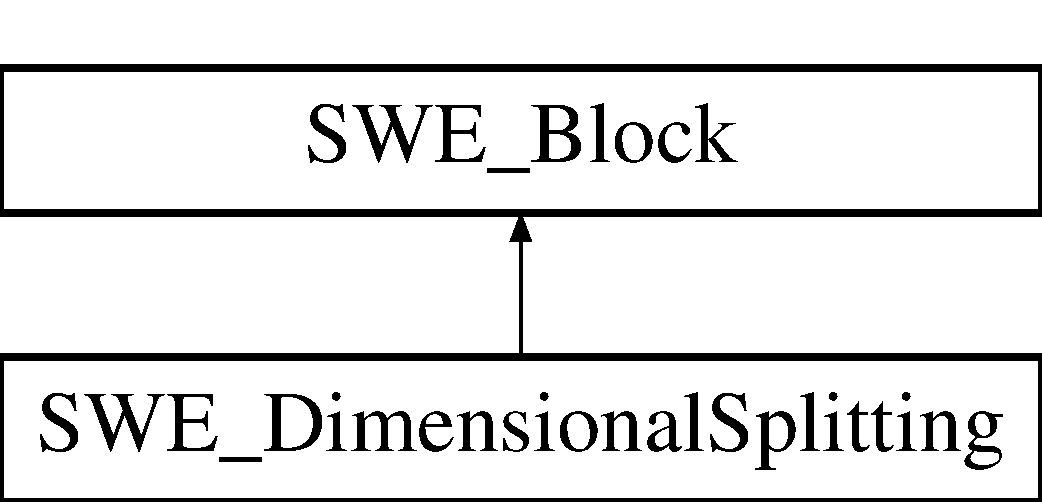
\includegraphics[height=2.000000cm]{classSWE__DimensionalSplitting}
\end{center}
\end{figure}
\subsection*{Public Member Functions}
\begin{DoxyCompactItemize}
\item 
{\bf S\-W\-E\-\_\-\-Dimensional\-Splitting} (int l\-\_\-nx, int l\-\_\-ny, float l\-\_\-dx, float l\-\_\-dy)
\item 
void {\bf compute\-Numerical\-Fluxes} ()
\item 
void {\bf update\-Unknowns} (float dt)
\item 
virtual {\bf $\sim$\-S\-W\-E\-\_\-\-Dimensional\-Splitting} ()
\end{DoxyCompactItemize}
\subsection*{Additional Inherited Members}


\subsection{Constructor \& Destructor Documentation}
\index{S\-W\-E\-\_\-\-Dimensional\-Splitting@{S\-W\-E\-\_\-\-Dimensional\-Splitting}!S\-W\-E\-\_\-\-Dimensional\-Splitting@{S\-W\-E\-\_\-\-Dimensional\-Splitting}}
\index{S\-W\-E\-\_\-\-Dimensional\-Splitting@{S\-W\-E\-\_\-\-Dimensional\-Splitting}!SWE_DimensionalSplitting@{S\-W\-E\-\_\-\-Dimensional\-Splitting}}
\subsubsection[{S\-W\-E\-\_\-\-Dimensional\-Splitting}]{\setlength{\rightskip}{0pt plus 5cm}S\-W\-E\-\_\-\-Dimensional\-Splitting\-::\-S\-W\-E\-\_\-\-Dimensional\-Splitting (
\begin{DoxyParamCaption}
\item[{int}]{l\-\_\-nx, }
\item[{int}]{l\-\_\-ny, }
\item[{float}]{l\-\_\-dx, }
\item[{float}]{l\-\_\-dy}
\end{DoxyParamCaption}
)}\label{classSWE__DimensionalSplitting_a3ab0c9de647ca241dbab1aa02cc42a04}
Constructor for \doxyref{S\-W\-E\-\_\-\-Dimensional\-Splitting}{p.}{classSWE__DimensionalSplitting} Declaring arrays and variables \index{S\-W\-E\-\_\-\-Dimensional\-Splitting@{S\-W\-E\-\_\-\-Dimensional\-Splitting}!$\sim$\-S\-W\-E\-\_\-\-Dimensional\-Splitting@{$\sim$\-S\-W\-E\-\_\-\-Dimensional\-Splitting}}
\index{$\sim$\-S\-W\-E\-\_\-\-Dimensional\-Splitting@{$\sim$\-S\-W\-E\-\_\-\-Dimensional\-Splitting}!SWE_DimensionalSplitting@{S\-W\-E\-\_\-\-Dimensional\-Splitting}}
\subsubsection[{$\sim$\-S\-W\-E\-\_\-\-Dimensional\-Splitting}]{\setlength{\rightskip}{0pt plus 5cm}S\-W\-E\-\_\-\-Dimensional\-Splitting\-::$\sim$\-S\-W\-E\-\_\-\-Dimensional\-Splitting (
\begin{DoxyParamCaption}
{}
\end{DoxyParamCaption}
)\hspace{0.3cm}{\ttfamily [virtual]}}\label{classSWE__DimensionalSplitting_a6679789a5063a15de688a9bed3686551}
Delete arrays and variables 

\subsection{Member Function Documentation}
\index{S\-W\-E\-\_\-\-Dimensional\-Splitting@{S\-W\-E\-\_\-\-Dimensional\-Splitting}!compute\-Numerical\-Fluxes@{compute\-Numerical\-Fluxes}}
\index{compute\-Numerical\-Fluxes@{compute\-Numerical\-Fluxes}!SWE_DimensionalSplitting@{S\-W\-E\-\_\-\-Dimensional\-Splitting}}
\subsubsection[{compute\-Numerical\-Fluxes}]{\setlength{\rightskip}{0pt plus 5cm}void S\-W\-E\-\_\-\-Dimensional\-Splitting\-::compute\-Numerical\-Fluxes (
\begin{DoxyParamCaption}
{}
\end{DoxyParamCaption}
)\hspace{0.3cm}{\ttfamily [virtual]}}\label{classSWE__DimensionalSplitting_a84759f8fbbbfe1e46613375515826f0f}
Compute numerical fluxes with x and y sweep for Task 3.\-2 

Implements {\bf S\-W\-E\-\_\-\-Block} \doxyref{}{p.}{classSWE__Block_a94dcf2c6ae31731e4586e45628b0c00e}.

\index{S\-W\-E\-\_\-\-Dimensional\-Splitting@{S\-W\-E\-\_\-\-Dimensional\-Splitting}!update\-Unknowns@{update\-Unknowns}}
\index{update\-Unknowns@{update\-Unknowns}!SWE_DimensionalSplitting@{S\-W\-E\-\_\-\-Dimensional\-Splitting}}
\subsubsection[{update\-Unknowns}]{\setlength{\rightskip}{0pt plus 5cm}void S\-W\-E\-\_\-\-Dimensional\-Splitting\-::update\-Unknowns (
\begin{DoxyParamCaption}
\item[{float}]{dt}
\end{DoxyParamCaption}
)\hspace{0.3cm}{\ttfamily [virtual]}}\label{classSWE__DimensionalSplitting_af74b527ff9ca7727442db92d2e438531}
Updateing height and momentum in x and y direction 

Implements {\bf S\-W\-E\-\_\-\-Block} \doxyref{}{p.}{classSWE__Block_ab2b4b659f23d5d45413dece8d2da3298}.



The documentation for this class was generated from the following files\-:\begin{DoxyCompactItemize}
\item 
src/blocks/{\bf S\-W\-E\-\_\-\-Block.\-hh}\item 
src/blocks/{\bf S\-W\-E\-\_\-\-Block.\-cpp}\end{DoxyCompactItemize}

\section{S\-W\-E\-\_\-\-Radial\-Dam\-Break\-Scenario Class Reference}
\label{classSWE__RadialDamBreakScenario}\index{S\-W\-E\-\_\-\-Radial\-Dam\-Break\-Scenario@{S\-W\-E\-\_\-\-Radial\-Dam\-Break\-Scenario}}


{\ttfamily \#include $<$S\-W\-E\-\_\-simple\-\_\-scenarios.\-hh$>$}

Inheritance diagram for S\-W\-E\-\_\-\-Radial\-Dam\-Break\-Scenario\-:\begin{figure}[H]
\begin{center}
\leavevmode
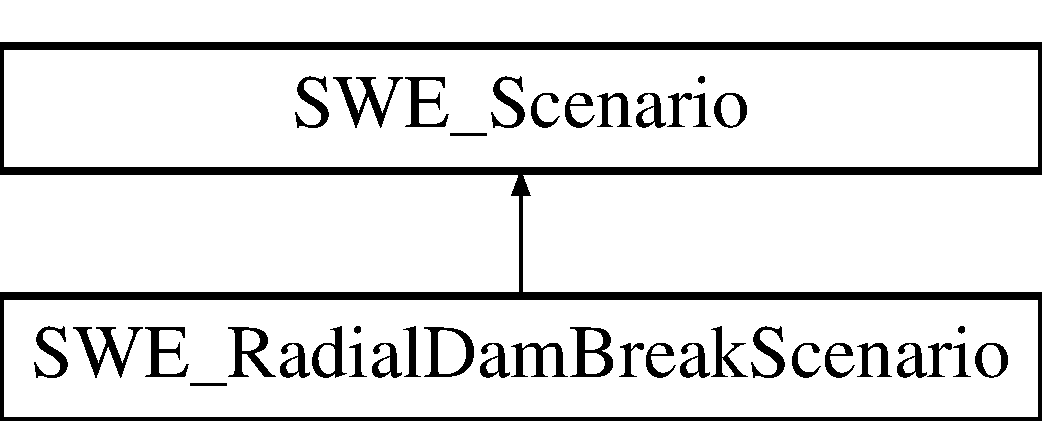
\includegraphics[height=2.000000cm]{classSWE__RadialDamBreakScenario}
\end{center}
\end{figure}
\subsection*{Public Member Functions}
\begin{DoxyCompactItemize}
\item 
float {\bfseries get\-Bathymetry} (float x, float y)\label{classSWE__RadialDamBreakScenario_ab54c88d18ff3a577a3e33f1659d97b50}

\item 
float {\bfseries get\-Water\-Height} (float x, float y)\label{classSWE__RadialDamBreakScenario_a0fb0917dd1e47f9580bd94ba5816795c}

\item 
virtual float {\bfseries end\-Simulation} ()\label{classSWE__RadialDamBreakScenario_a5e118a3d34aace3175745965d5d9c567}

\item 
virtual {\bf Boundary\-Type} {\bfseries get\-Boundary\-Type} ({\bf Boundary\-Edge} edge)\label{classSWE__RadialDamBreakScenario_a40a7ddfd7d85631eeb708232c9f7f20d}

\item 
float {\bf get\-Boundary\-Pos} ({\bf Boundary\-Edge} i\-\_\-edge)
\end{DoxyCompactItemize}


\subsection{Detailed Description}
Scenario \char`\"{}\-Radial Dam Break\char`\"{}\-: elevated water in the center of the domain 

\subsection{Member Function Documentation}
\index{S\-W\-E\-\_\-\-Radial\-Dam\-Break\-Scenario@{S\-W\-E\-\_\-\-Radial\-Dam\-Break\-Scenario}!get\-Boundary\-Pos@{get\-Boundary\-Pos}}
\index{get\-Boundary\-Pos@{get\-Boundary\-Pos}!SWE_RadialDamBreakScenario@{S\-W\-E\-\_\-\-Radial\-Dam\-Break\-Scenario}}
\subsubsection[{get\-Boundary\-Pos}]{\setlength{\rightskip}{0pt plus 5cm}float S\-W\-E\-\_\-\-Radial\-Dam\-Break\-Scenario\-::get\-Boundary\-Pos (
\begin{DoxyParamCaption}
\item[{{\bf Boundary\-Edge}}]{i\-\_\-edge}
\end{DoxyParamCaption}
)\hspace{0.3cm}{\ttfamily [inline]}, {\ttfamily [virtual]}}\label{classSWE__RadialDamBreakScenario_ac5392df630c8164560df5cb902df385a}
Get the boundary positions


\begin{DoxyParams}{Parameters}
{\em i\-\_\-edge} & which edge \\
\hline
\end{DoxyParams}
\begin{DoxyReturn}{Returns}
value in the corresponding dimension 
\end{DoxyReturn}


Reimplemented from {\bf S\-W\-E\-\_\-\-Scenario} \doxyref{}{p.}{classSWE__Scenario}.



The documentation for this class was generated from the following file\-:\begin{DoxyCompactItemize}
\item 
src/scenarios/{\bf S\-W\-E\-\_\-simple\-\_\-scenarios.\-hh}\end{DoxyCompactItemize}

\section{S\-W\-E\-\_\-\-Rusanov\-Block Class Reference}
\label{classSWE__RusanovBlock}\index{S\-W\-E\-\_\-\-Rusanov\-Block@{S\-W\-E\-\_\-\-Rusanov\-Block}}


{\ttfamily \#include $<$S\-W\-E\-\_\-\-Rusanov\-Block.\-hh$>$}

Inheritance diagram for S\-W\-E\-\_\-\-Rusanov\-Block\-:\begin{figure}[H]
\begin{center}
\leavevmode
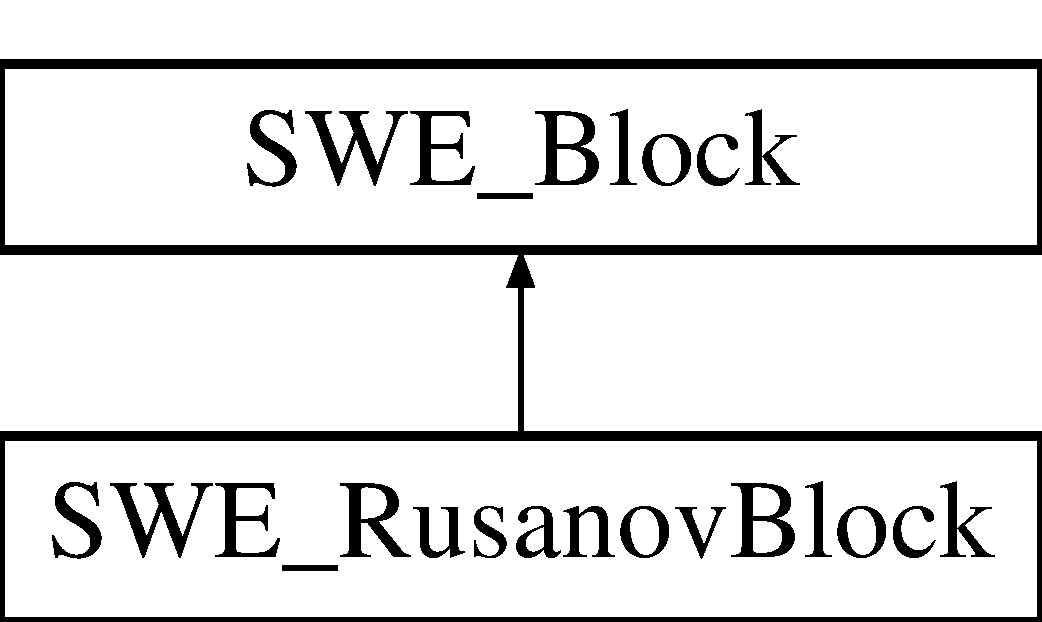
\includegraphics[height=2.000000cm]{classSWE__RusanovBlock}
\end{center}
\end{figure}
\subsection*{Public Member Functions}
\begin{DoxyCompactItemize}
\item 
{\bf S\-W\-E\-\_\-\-Rusanov\-Block} (float \-\_\-offset\-X=0, float \-\_\-offset\-Y=0)
\item 
virtual {\bf $\sim$\-S\-W\-E\-\_\-\-Rusanov\-Block} ()
\item 
virtual void {\bf simulate\-Timestep} (float dt)
\begin{DoxyCompactList}\small\item\em execute a single time step of the simulation \end{DoxyCompactList}\item 
virtual float {\bf simulate} (float t\-Start, float t\-End)
\begin{DoxyCompactList}\small\item\em compute simulate from specified start to end time \end{DoxyCompactList}\item 
virtual void {\bf compute\-Numerical\-Fluxes} ()
\begin{DoxyCompactList}\small\item\em compute flux terms on edges \end{DoxyCompactList}\item 
virtual void {\bf update\-Unknowns} (float dt)
\begin{DoxyCompactList}\small\item\em update unknowns according to fluxes (Euler time step) \end{DoxyCompactList}\end{DoxyCompactItemize}
\subsection*{Protected Member Functions}
\begin{DoxyCompactItemize}
\item 
virtual void {\bf compute\-Bathymetry\-Sources} ()
\begin{DoxyCompactList}\small\item\em compute source terms \end{DoxyCompactList}\item 
float {\bf compute\-Local\-S\-V} (int i, int j, char dir)
\item 
virtual void {\bfseries compute\-Max\-Timestep} ()\label{classSWE__RusanovBlock_a88b3537e5dbe509b0b7495b8e28275bf}

\end{DoxyCompactItemize}
\subsection*{Static Protected Member Functions}
\begin{DoxyCompactItemize}
\item 
static float {\bf compute\-Flux} (float f\-Loc, float f\-Neigh, float xi\-Loc, float xi\-Neigh, float llf)
\end{DoxyCompactItemize}
\subsection*{Protected Attributes}
\begin{DoxyCompactItemize}
\item 
{\bf Float2\-D} {\bfseries Fh}\label{classSWE__RusanovBlock_a13e147a6a4f8b39e1a95f37372a04d5b}

\item 
{\bf Float2\-D} {\bfseries Fhu}\label{classSWE__RusanovBlock_a945f257acfa7b05dd0989c9525160b0b}

\item 
{\bf Float2\-D} {\bfseries Fhv}\label{classSWE__RusanovBlock_a788982f2b64f97d271291ef7df669c57}

\item 
{\bf Float2\-D} {\bfseries Gh}\label{classSWE__RusanovBlock_aaa1d9c2b8f3dc1afe0f818bade7c3940}

\item 
{\bf Float2\-D} {\bfseries Ghu}\label{classSWE__RusanovBlock_af479e7882925550951da40ce85736f83}

\item 
{\bf Float2\-D} {\bfseries Ghv}\label{classSWE__RusanovBlock_a2f856e0d68708748451c9ca1f166aa79}

\item 
{\bf Float2\-D} {\bfseries Bx}\label{classSWE__RusanovBlock_af6f73bf8459849ad75c1d7e70b279710}

\item 
{\bf Float2\-D} {\bfseries By}\label{classSWE__RusanovBlock_a0c044eadcc80059b8708cf8f8c77add1}

\end{DoxyCompactItemize}
\subsection*{Friends}
\begin{DoxyCompactItemize}
\item 
ostream \& {\bf operator$<$$<$} (ostream \&os, const {\bf S\-W\-E\-\_\-\-Rusanov\-Block} \&swe)
\end{DoxyCompactItemize}
\subsection*{Additional Inherited Members}


\subsection{Detailed Description}
\doxyref{S\-W\-E\-\_\-\-Rusanov\-Block}{p.}{classSWE__RusanovBlock} is an implementation of the \doxyref{S\-W\-E\-\_\-\-Block}{p.}{classSWE__Block} abstract class. It uses a simple Rusanov flux (aka local Lax-\/\-Friedrich) in the model, with some simple modifications to obtain a well-\/balanced scheme. 

\subsection{Constructor \& Destructor Documentation}
\index{S\-W\-E\-\_\-\-Rusanov\-Block@{S\-W\-E\-\_\-\-Rusanov\-Block}!S\-W\-E\-\_\-\-Rusanov\-Block@{S\-W\-E\-\_\-\-Rusanov\-Block}}
\index{S\-W\-E\-\_\-\-Rusanov\-Block@{S\-W\-E\-\_\-\-Rusanov\-Block}!SWE_RusanovBlock@{S\-W\-E\-\_\-\-Rusanov\-Block}}
\subsubsection[{S\-W\-E\-\_\-\-Rusanov\-Block}]{\setlength{\rightskip}{0pt plus 5cm}S\-W\-E\-\_\-\-Rusanov\-Block\-::\-S\-W\-E\-\_\-\-Rusanov\-Block (
\begin{DoxyParamCaption}
\item[{float}]{\-\_\-offset\-X = {\ttfamily 0}, }
\item[{float}]{\-\_\-offset\-Y = {\ttfamily 0}}
\end{DoxyParamCaption}
)}\label{classSWE__RusanovBlock_a479a282899300076c44ccabcb42b5b5c}
Constructor\-: allocate variables for simulation

unknowns h,hu,hv,b are defined on grid indices [0,..,nx+1]$\ast$[0,..,ny+1] -\/$>$ computational domain is [1,..,nx]$\ast$[1,..,ny] -\/$>$ plus ghost cell layer

flux terms are defined for edges with indices [0,..,nx]$\ast$[1,..,ny] or [1,..,nx]$\ast${\tt 0,..,ny} Flux term with index (i,j) is located on the edge between cells with index (i,j) and (i+1,j) or (i,j+1)

bathymetry source terms are defined for cells with indices [1,..,nx]$\ast$[1,..,ny]

@ param \-\_\-offset\-X x coordinate of block origin @ param \-\_\-offset\-Y y coordinate of block origin \index{S\-W\-E\-\_\-\-Rusanov\-Block@{S\-W\-E\-\_\-\-Rusanov\-Block}!$\sim$\-S\-W\-E\-\_\-\-Rusanov\-Block@{$\sim$\-S\-W\-E\-\_\-\-Rusanov\-Block}}
\index{$\sim$\-S\-W\-E\-\_\-\-Rusanov\-Block@{$\sim$\-S\-W\-E\-\_\-\-Rusanov\-Block}!SWE_RusanovBlock@{S\-W\-E\-\_\-\-Rusanov\-Block}}
\subsubsection[{$\sim$\-S\-W\-E\-\_\-\-Rusanov\-Block}]{\setlength{\rightskip}{0pt plus 5cm}S\-W\-E\-\_\-\-Rusanov\-Block\-::$\sim$\-S\-W\-E\-\_\-\-Rusanov\-Block (
\begin{DoxyParamCaption}
{}
\end{DoxyParamCaption}
)\hspace{0.3cm}{\ttfamily [virtual]}}\label{classSWE__RusanovBlock_aab12f79b94c8ac3cc541ceb2814f72d4}
Destructor\-: de-\/allocate all variables 

\subsection{Member Function Documentation}
\index{S\-W\-E\-\_\-\-Rusanov\-Block@{S\-W\-E\-\_\-\-Rusanov\-Block}!compute\-Bathymetry\-Sources@{compute\-Bathymetry\-Sources}}
\index{compute\-Bathymetry\-Sources@{compute\-Bathymetry\-Sources}!SWE_RusanovBlock@{S\-W\-E\-\_\-\-Rusanov\-Block}}
\subsubsection[{compute\-Bathymetry\-Sources}]{\setlength{\rightskip}{0pt plus 5cm}void S\-W\-E\-\_\-\-Rusanov\-Block\-::compute\-Bathymetry\-Sources (
\begin{DoxyParamCaption}
{}
\end{DoxyParamCaption}
)\hspace{0.3cm}{\ttfamily [protected]}, {\ttfamily [virtual]}}\label{classSWE__RusanovBlock_ac7306305d9c39e418301fc588693c88b}


compute source terms 

compute the bathymetry source terms in all cells \index{S\-W\-E\-\_\-\-Rusanov\-Block@{S\-W\-E\-\_\-\-Rusanov\-Block}!compute\-Flux@{compute\-Flux}}
\index{compute\-Flux@{compute\-Flux}!SWE_RusanovBlock@{S\-W\-E\-\_\-\-Rusanov\-Block}}
\subsubsection[{compute\-Flux}]{\setlength{\rightskip}{0pt plus 5cm}float S\-W\-E\-\_\-\-Rusanov\-Block\-::compute\-Flux (
\begin{DoxyParamCaption}
\item[{float}]{f\-Low, }
\item[{float}]{f\-High, }
\item[{float}]{xi\-Low, }
\item[{float}]{xi\-High, }
\item[{float}]{llf}
\end{DoxyParamCaption}
)\hspace{0.3cm}{\ttfamily [static]}, {\ttfamily [protected]}}\label{classSWE__RusanovBlock_a37c4e0d841054a32adaa8ab26fb7c208}
compute the flux term on a given edge (acc. to local Lax-\/\-Friedrich method aka Rusanov flux)\-: f\-Low and f\-High contain the values of the flux function in the two adjacent grid cells xi\-Low and xi\-High are the values of the unknowns in the two adjacent grid cells \char`\"{}\-Low\char`\"{} represents the cell with lower i/j index (\char`\"{}\-High\char`\"{} for larger index). llf should contain the local signal velocity (as compute by compute\-Local\-S\-V) for llf=dx/dt (or dy/dt), we obtain the standard Lax Friedrich method \index{S\-W\-E\-\_\-\-Rusanov\-Block@{S\-W\-E\-\_\-\-Rusanov\-Block}!compute\-Local\-S\-V@{compute\-Local\-S\-V}}
\index{compute\-Local\-S\-V@{compute\-Local\-S\-V}!SWE_RusanovBlock@{S\-W\-E\-\_\-\-Rusanov\-Block}}
\subsubsection[{compute\-Local\-S\-V}]{\setlength{\rightskip}{0pt plus 5cm}float S\-W\-E\-\_\-\-Rusanov\-Block\-::compute\-Local\-S\-V (
\begin{DoxyParamCaption}
\item[{int}]{i, }
\item[{int}]{j, }
\item[{char}]{dir}
\end{DoxyParamCaption}
)\hspace{0.3cm}{\ttfamily [protected]}}\label{classSWE__RusanovBlock_a5a2f154dd2110e8515829564dd806530}
computes the local signal velocity in x-\/ or y-\/direction for two adjacent cells with indices (i,j) and (i+1,j) (if dir='x') or (i,j+1) (if dir='y' \index{S\-W\-E\-\_\-\-Rusanov\-Block@{S\-W\-E\-\_\-\-Rusanov\-Block}!compute\-Numerical\-Fluxes@{compute\-Numerical\-Fluxes}}
\index{compute\-Numerical\-Fluxes@{compute\-Numerical\-Fluxes}!SWE_RusanovBlock@{S\-W\-E\-\_\-\-Rusanov\-Block}}
\subsubsection[{compute\-Numerical\-Fluxes}]{\setlength{\rightskip}{0pt plus 5cm}void S\-W\-E\-\_\-\-Rusanov\-Block\-::compute\-Numerical\-Fluxes (
\begin{DoxyParamCaption}
{}
\end{DoxyParamCaption}
)\hspace{0.3cm}{\ttfamily [virtual]}}\label{classSWE__RusanovBlock_a78cdefa510cd2d88ca4e213f75b9b10b}


compute flux terms on edges 

compute the flux terms on all edges; before the computation, compute\-Bathymetry\-Sources is called 

Implements {\bf S\-W\-E\-\_\-\-Block} \doxyref{}{p.}{classSWE__Block_a94dcf2c6ae31731e4586e45628b0c00e}.

\index{S\-W\-E\-\_\-\-Rusanov\-Block@{S\-W\-E\-\_\-\-Rusanov\-Block}!simulate@{simulate}}
\index{simulate@{simulate}!SWE_RusanovBlock@{S\-W\-E\-\_\-\-Rusanov\-Block}}
\subsubsection[{simulate}]{\setlength{\rightskip}{0pt plus 5cm}float S\-W\-E\-\_\-\-Rusanov\-Block\-::simulate (
\begin{DoxyParamCaption}
\item[{float}]{t\-Start, }
\item[{float}]{t\-End}
\end{DoxyParamCaption}
)\hspace{0.3cm}{\ttfamily [virtual]}}\label{classSWE__RusanovBlock_a645322106b3e5b6f0cca077611ad2159}


compute simulate from specified start to end time 

implements interface function simulate\-: perform forward-\/\-Euler time steps, starting with simulation time t\-Start,\-: until simulation time t\-End is reached; boundary conditions and bathymetry source terms are computed for each timestep as required -\/ intended as main simulation loop between two checkpoints 

Reimplemented from {\bf S\-W\-E\-\_\-\-Block} \doxyref{}{p.}{classSWE__Block_a69784e2be2d09035fb2af9d306768f07}.

\index{S\-W\-E\-\_\-\-Rusanov\-Block@{S\-W\-E\-\_\-\-Rusanov\-Block}!simulate\-Timestep@{simulate\-Timestep}}
\index{simulate\-Timestep@{simulate\-Timestep}!SWE_RusanovBlock@{S\-W\-E\-\_\-\-Rusanov\-Block}}
\subsubsection[{simulate\-Timestep}]{\setlength{\rightskip}{0pt plus 5cm}void S\-W\-E\-\_\-\-Rusanov\-Block\-::simulate\-Timestep (
\begin{DoxyParamCaption}
\item[{float}]{dt}
\end{DoxyParamCaption}
)\hspace{0.3cm}{\ttfamily [virtual]}}\label{classSWE__RusanovBlock_ada062db4f54700011d50378b0045830a}


execute a single time step of the simulation 

Depending on the current values of h, hu, hv (incl. ghost layers) update these unknowns in each grid cell (ghost layers and bathymetry are not updated). The Rusanov implementation of simulate\-Timestep subsequently calls the functions compute\-Numerical\-Fluxes (to compute all fluxes on grid edges), and update\-Unknowns (to update the variables according to flux values, typically according to an Euler time step). 
\begin{DoxyParams}{Parameters}
{\em dt} & size of the time step \\
\hline
\end{DoxyParams}


Reimplemented from {\bf S\-W\-E\-\_\-\-Block} \doxyref{}{p.}{classSWE__Block_add6908e1ceb261a0a1f3ebc262cc5f11}.

\index{S\-W\-E\-\_\-\-Rusanov\-Block@{S\-W\-E\-\_\-\-Rusanov\-Block}!update\-Unknowns@{update\-Unknowns}}
\index{update\-Unknowns@{update\-Unknowns}!SWE_RusanovBlock@{S\-W\-E\-\_\-\-Rusanov\-Block}}
\subsubsection[{update\-Unknowns}]{\setlength{\rightskip}{0pt plus 5cm}void S\-W\-E\-\_\-\-Rusanov\-Block\-::update\-Unknowns (
\begin{DoxyParamCaption}
\item[{float}]{dt}
\end{DoxyParamCaption}
)\hspace{0.3cm}{\ttfamily [virtual]}}\label{classSWE__RusanovBlock_a2980aa21030ba8fc607001ad817d7454}


update unknowns according to fluxes (Euler time step) 

implements interface function update\-Unknowns\-: based on the (Rusanov) fluxes computed on each edge (and stored in the variables Fh, Gh, etc.); compute the balance terms for each cell, and update the unknowns according to an Euler time step. 
\begin{DoxyParams}{Parameters}
{\em dt} & size of the time step. \\
\hline
\end{DoxyParams}


Implements {\bf S\-W\-E\-\_\-\-Block} \doxyref{}{p.}{classSWE__Block_ab2b4b659f23d5d45413dece8d2da3298}.



\subsection{Friends And Related Function Documentation}
\index{S\-W\-E\-\_\-\-Rusanov\-Block@{S\-W\-E\-\_\-\-Rusanov\-Block}!operator$<$$<$@{operator$<$$<$}}
\index{operator$<$$<$@{operator$<$$<$}!SWE_RusanovBlock@{S\-W\-E\-\_\-\-Rusanov\-Block}}
\subsubsection[{operator$<$$<$}]{\setlength{\rightskip}{0pt plus 5cm}ostream\& operator$<$$<$ (
\begin{DoxyParamCaption}
\item[{ostream \&}]{os, }
\item[{const {\bf S\-W\-E\-\_\-\-Rusanov\-Block} \&}]{swe}
\end{DoxyParamCaption}
)\hspace{0.3cm}{\ttfamily [friend]}}\label{classSWE__RusanovBlock_a11f96afabd5e590e50d491568b96503a}
overload operator$<$$<$ such that data can be written via cout $<$$<$ -\/$>$ needs to be declared as friend to be allowed to access private data 

The documentation for this class was generated from the following files\-:\begin{DoxyCompactItemize}
\item 
src/blocks/rusanov/{\bf S\-W\-E\-\_\-\-Rusanov\-Block.\-hh}\item 
src/blocks/rusanov/{\bf S\-W\-E\-\_\-\-Rusanov\-Block.\-cpp}\end{DoxyCompactItemize}

\section{S\-W\-E\-\_\-\-Rusanov\-Block\-C\-U\-D\-A Class Reference}
\label{classSWE__RusanovBlockCUDA}\index{S\-W\-E\-\_\-\-Rusanov\-Block\-C\-U\-D\-A@{S\-W\-E\-\_\-\-Rusanov\-Block\-C\-U\-D\-A}}


{\ttfamily \#include $<$S\-W\-E\-\_\-\-Rusanov\-Block\-C\-U\-D\-A.\-hh$>$}

Inheritance diagram for S\-W\-E\-\_\-\-Rusanov\-Block\-C\-U\-D\-A\-:\begin{figure}[H]
\begin{center}
\leavevmode
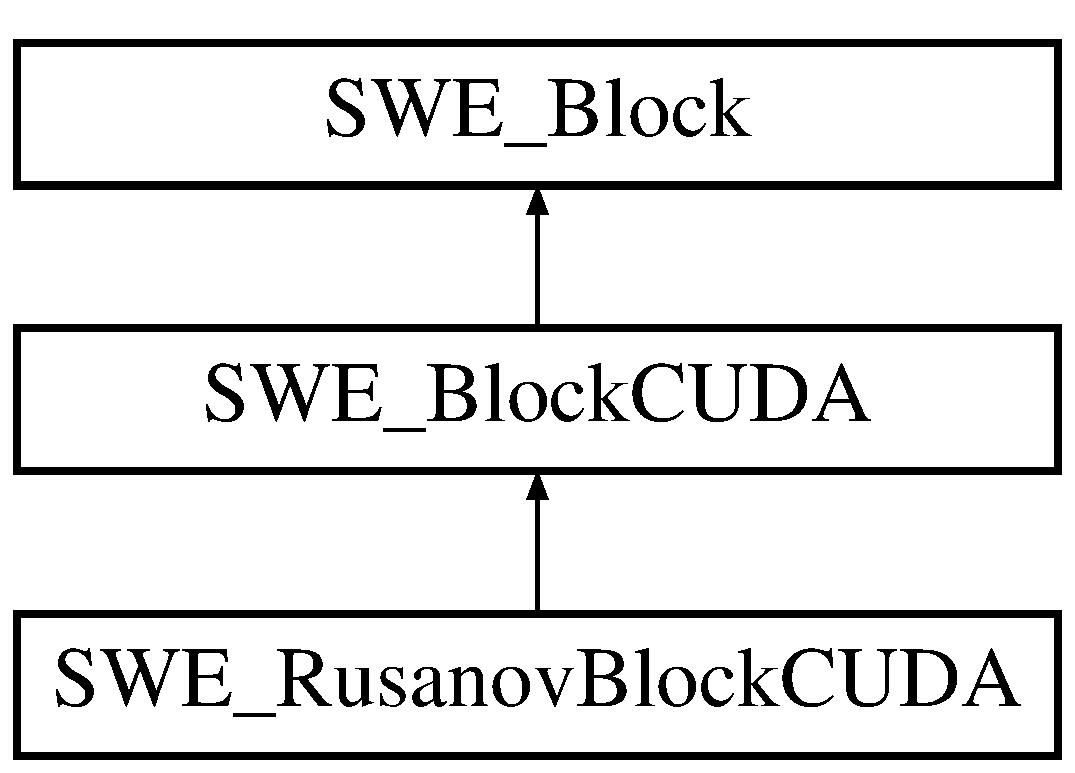
\includegraphics[height=3.000000cm]{classSWE__RusanovBlockCUDA}
\end{center}
\end{figure}
\subsection*{Public Member Functions}
\begin{DoxyCompactItemize}
\item 
{\bfseries S\-W\-E\-\_\-\-Rusanov\-Block\-C\-U\-D\-A} (float \-\_\-offset\-X=0, float \-\_\-offset\-Y=0, const int i\-\_\-cuda\-Device=0)\label{classSWE__RusanovBlockCUDA_a5bd6db4a52d816534923d851ea6f9314}

\item 
virtual void {\bf compute\-Numerical\-Fluxes} ()
\begin{DoxyCompactList}\small\item\em compute the numerical fluxes for each edge of the Cartesian grid \end{DoxyCompactList}\item 
virtual void {\bf update\-Unknowns} (float dt)
\begin{DoxyCompactList}\small\item\em compute the new values of the unknowns h, hu, and hv in all grid cells \end{DoxyCompactList}\item 
virtual void {\bf simulate\-Timestep} (float dt)\label{classSWE__RusanovBlockCUDA_aa039b202a505cf31ab16e8c74dc4153b}

\begin{DoxyCompactList}\small\item\em execute a single time step of the simulation \end{DoxyCompactList}\item 
virtual float {\bf simulate} (float t\-Start, float t\-End)
\end{DoxyCompactItemize}
\subsection*{Friends}
\begin{DoxyCompactItemize}
\item 
ostream \& {\bfseries operator$<$$<$} (ostream \&os, const {\bf S\-W\-E\-\_\-\-Rusanov\-Block\-C\-U\-D\-A} \&swe)\label{classSWE__RusanovBlockCUDA_adbdcb6417643b695657724ea16f84954}

\end{DoxyCompactItemize}
\subsection*{Additional Inherited Members}


\subsection{Detailed Description}
\doxyref{S\-W\-E\-\_\-\-Rusanov\-Block\-C\-U\-D\-A}{p.}{classSWE__RusanovBlockCUDA} extends the base class \doxyref{S\-W\-E\-\_\-\-Block\-C\-U\-D\-A}{p.}{classSWE__BlockCUDA}, and provides a concrete C\-U\-D\-A implementation of a simple shallow water model based on Rusanov Flux computation on the edges and explicit time stepping. 

\subsection{Member Function Documentation}
\index{S\-W\-E\-\_\-\-Rusanov\-Block\-C\-U\-D\-A@{S\-W\-E\-\_\-\-Rusanov\-Block\-C\-U\-D\-A}!compute\-Numerical\-Fluxes@{compute\-Numerical\-Fluxes}}
\index{compute\-Numerical\-Fluxes@{compute\-Numerical\-Fluxes}!SWE_RusanovBlockCUDA@{S\-W\-E\-\_\-\-Rusanov\-Block\-C\-U\-D\-A}}
\subsubsection[{compute\-Numerical\-Fluxes}]{\setlength{\rightskip}{0pt plus 5cm}virtual void S\-W\-E\-\_\-\-Rusanov\-Block\-C\-U\-D\-A\-::compute\-Numerical\-Fluxes (
\begin{DoxyParamCaption}
{}
\end{DoxyParamCaption}
)\hspace{0.3cm}{\ttfamily [virtual]}}\label{classSWE__RusanovBlockCUDA_a64fa005a8f69f49ac7894dffcec39787}


compute the numerical fluxes for each edge of the Cartesian grid 

The computation of fluxes strongly depends on the chosen numerical method. Hence, this purely virtual function has to be implemented in the respective derived classes. 

Implements {\bf S\-W\-E\-\_\-\-Block} \doxyref{}{p.}{classSWE__Block_a94dcf2c6ae31731e4586e45628b0c00e}.

\index{S\-W\-E\-\_\-\-Rusanov\-Block\-C\-U\-D\-A@{S\-W\-E\-\_\-\-Rusanov\-Block\-C\-U\-D\-A}!simulate@{simulate}}
\index{simulate@{simulate}!SWE_RusanovBlockCUDA@{S\-W\-E\-\_\-\-Rusanov\-Block\-C\-U\-D\-A}}
\subsubsection[{simulate}]{\setlength{\rightskip}{0pt plus 5cm}virtual float S\-W\-E\-\_\-\-Rusanov\-Block\-C\-U\-D\-A\-::simulate (
\begin{DoxyParamCaption}
\item[{float}]{i\-\_\-t\-Start, }
\item[{float}]{i\-\_\-t\-End}
\end{DoxyParamCaption}
)\hspace{0.3cm}{\ttfamily [virtual]}}\label{classSWE__RusanovBlockCUDA_a42c63cf7d3c5609768aa28263393efb6}
perform the simulation starting with simulation time t\-Start, until simulation time t\-End is reached

simulate implements the main simulation loop between two checkpoints; Note\-: this implementation can only be used, if you only use a single \doxyref{S\-W\-E\-\_\-\-Block}{p.}{classSWE__Block} and only apply simple boundary conditions! In particular, \doxyref{S\-W\-E\-\_\-\-Block\-::simulate}{p.}{classSWE__Block_a69784e2be2d09035fb2af9d306768f07} can not trigger calls to exchange values of copy and ghost layers between blocks! 
\begin{DoxyParams}{Parameters}
{\em t\-Start} & time where the simulation is started \\
\hline
{\em t\-End} & time of the next checkpoint \\
\hline
\end{DoxyParams}
\begin{DoxyReturn}{Returns}
actual end time reached 
\end{DoxyReturn}


Reimplemented from {\bf S\-W\-E\-\_\-\-Block} \doxyref{}{p.}{classSWE__Block_a69784e2be2d09035fb2af9d306768f07}.

\index{S\-W\-E\-\_\-\-Rusanov\-Block\-C\-U\-D\-A@{S\-W\-E\-\_\-\-Rusanov\-Block\-C\-U\-D\-A}!update\-Unknowns@{update\-Unknowns}}
\index{update\-Unknowns@{update\-Unknowns}!SWE_RusanovBlockCUDA@{S\-W\-E\-\_\-\-Rusanov\-Block\-C\-U\-D\-A}}
\subsubsection[{update\-Unknowns}]{\setlength{\rightskip}{0pt plus 5cm}virtual void S\-W\-E\-\_\-\-Rusanov\-Block\-C\-U\-D\-A\-::update\-Unknowns (
\begin{DoxyParamCaption}
\item[{float}]{dt}
\end{DoxyParamCaption}
)\hspace{0.3cm}{\ttfamily [virtual]}}\label{classSWE__RusanovBlockCUDA_a037264d8f044fd4d323420562c82a218}


compute the new values of the unknowns h, hu, and hv in all grid cells 

based on the numerical fluxes (computed by compute\-Numerical\-Fluxes) and the specified time step size dt, an Euler time step is executed. As the computational fluxes will depend on the numerical method, this purely virtual function has to be implemented separately for each specific numerical model (and parallelisation approach). 
\begin{DoxyParams}{Parameters}
{\em dt} & size of the time step \\
\hline
\end{DoxyParams}


Implements {\bf S\-W\-E\-\_\-\-Block} \doxyref{}{p.}{classSWE__Block_ab2b4b659f23d5d45413dece8d2da3298}.



The documentation for this class was generated from the following file\-:\begin{DoxyCompactItemize}
\item 
src/blocks/rusanov/{\bf S\-W\-E\-\_\-\-Rusanov\-Block\-C\-U\-D\-A.\-hh}\end{DoxyCompactItemize}

\section{S\-W\-E\-\_\-\-Scenario Class Reference}
\label{classSWE__Scenario}\index{S\-W\-E\-\_\-\-Scenario@{S\-W\-E\-\_\-\-Scenario}}


{\ttfamily \#include $<$S\-W\-E\-\_\-\-Scenario.\-hh$>$}

Inheritance diagram for S\-W\-E\-\_\-\-Scenario\-:\begin{figure}[H]
\begin{center}
\leavevmode
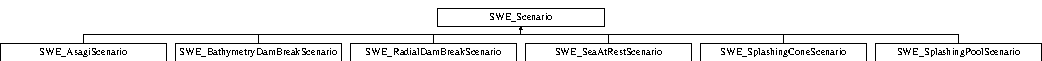
\includegraphics[height=0.825959cm]{classSWE__Scenario}
\end{center}
\end{figure}
\subsection*{Public Member Functions}
\begin{DoxyCompactItemize}
\item 
virtual float {\bfseries get\-Water\-Height} (float x, float y)\label{classSWE__Scenario_ade6f356d60b1402c034611266462b88b}

\item 
virtual float {\bfseries get\-Veloc\-\_\-u} (float x, float y)\label{classSWE__Scenario_ab1d5e360c861df3c8c0ccd919bd7f495}

\item 
virtual float {\bfseries get\-Veloc\-\_\-v} (float x, float y)\label{classSWE__Scenario_afeaf75872a1678ea64e6f7accd1e49c6}

\item 
virtual float {\bfseries get\-Bathymetry} (float x, float y)\label{classSWE__Scenario_afe09a1ba63304800651f25873570a348}

\item 
virtual float {\bfseries water\-Height\-At\-Rest} ()\label{classSWE__Scenario_a9de0f0f9fcc34dfe00c522b10c343d91}

\item 
virtual float {\bfseries end\-Simulation} ()\label{classSWE__Scenario_ae7ed72f584069e9885c33c4ca83f3ff5}

\item 
virtual {\bf Boundary\-Type} {\bfseries get\-Boundary\-Type} ({\bf Boundary\-Edge} edge)\label{classSWE__Scenario_ab8fe7ce15d7758fb0c4e0e3887b34a5d}

\item 
virtual float {\bfseries get\-Boundary\-Pos} ({\bf Boundary\-Edge} edge)\label{classSWE__Scenario_a1b01e953c2079b64f527c9bc5a0c86d7}

\end{DoxyCompactItemize}


\subsection{Detailed Description}
\doxyref{S\-W\-E\-\_\-\-Scenario}{p.}{classSWE__Scenario} defines an interface to initialise the unknowns of a shallow water simulation -\/ i.\-e. to initialise water height, velocities, and bathymatry according to certain scenarios. \doxyref{S\-W\-E\-\_\-\-Scenario}{p.}{classSWE__Scenario} can act as stand-\/alone scenario class, providing a very basic scenario (all functions are constant); however, the idea is to provide derived classes that implement the \doxyref{S\-W\-E\-\_\-\-Scenario}{p.}{classSWE__Scenario} interface for more interesting scenarios. 

The documentation for this class was generated from the following file\-:\begin{DoxyCompactItemize}
\item 
src/scenarios/{\bf S\-W\-E\-\_\-\-Scenario.\-hh}\end{DoxyCompactItemize}

\section{S\-W\-E\-\_\-\-Sea\-At\-Rest\-Scenario Class Reference}
\label{classSWE__SeaAtRestScenario}\index{S\-W\-E\-\_\-\-Sea\-At\-Rest\-Scenario@{S\-W\-E\-\_\-\-Sea\-At\-Rest\-Scenario}}


{\ttfamily \#include $<$S\-W\-E\-\_\-simple\-\_\-scenarios.\-hh$>$}

Inheritance diagram for S\-W\-E\-\_\-\-Sea\-At\-Rest\-Scenario\-:\begin{figure}[H]
\begin{center}
\leavevmode
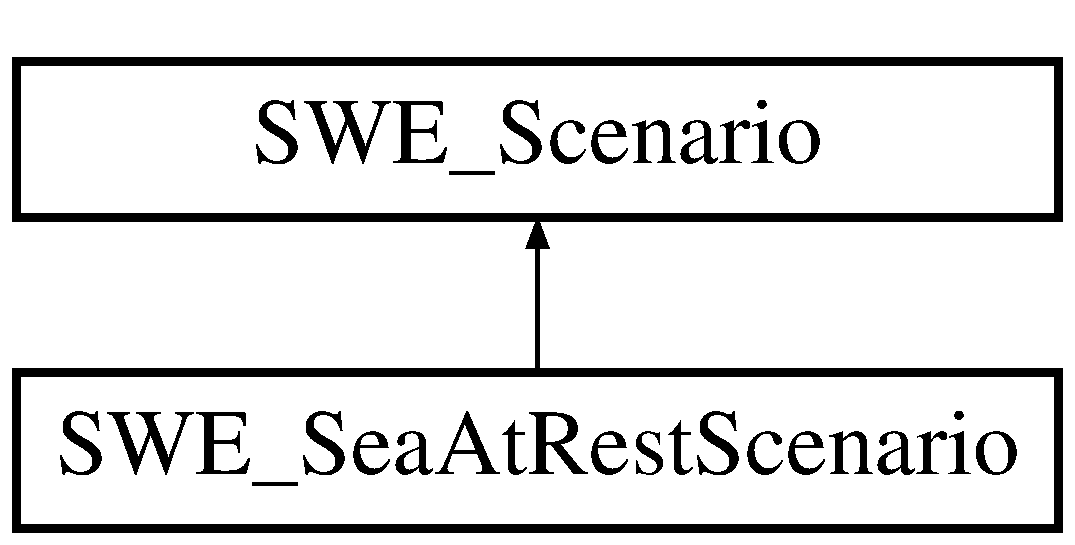
\includegraphics[height=2.000000cm]{classSWE__SeaAtRestScenario}
\end{center}
\end{figure}
\subsection*{Public Member Functions}
\begin{DoxyCompactItemize}
\item 
float {\bfseries get\-Water\-Height} (float x, float y)\label{classSWE__SeaAtRestScenario_a0d493a2c96cde62cc71035c5f62717d1}

\item 
float {\bfseries get\-Bathymetry} (float x, float y)\label{classSWE__SeaAtRestScenario_a738776f758bb5b914ede2e6f57cb3ffd}

\end{DoxyCompactItemize}


\subsection{Detailed Description}
Scenario \char`\"{}\-Sea at Rest\char`\"{}\-: flat water surface (\char`\"{}sea at rest\char`\"{}), but non-\/uniform bathymetry (id. to \char`\"{}\-Bathymetry Dam Break\char`\"{}) test scenario for \char`\"{}sea at rest\char`\"{}-\/solution 

The documentation for this class was generated from the following file\-:\begin{DoxyCompactItemize}
\item 
src/scenarios/{\bf S\-W\-E\-\_\-simple\-\_\-scenarios.\-hh}\end{DoxyCompactItemize}

\section{S\-W\-E\-\_\-\-Splashing\-Cone\-Scenario Class Reference}
\label{classSWE__SplashingConeScenario}\index{S\-W\-E\-\_\-\-Splashing\-Cone\-Scenario@{S\-W\-E\-\_\-\-Splashing\-Cone\-Scenario}}


{\ttfamily \#include $<$S\-W\-E\-\_\-simple\-\_\-scenarios.\-hh$>$}

Inheritance diagram for S\-W\-E\-\_\-\-Splashing\-Cone\-Scenario\-:\begin{figure}[H]
\begin{center}
\leavevmode
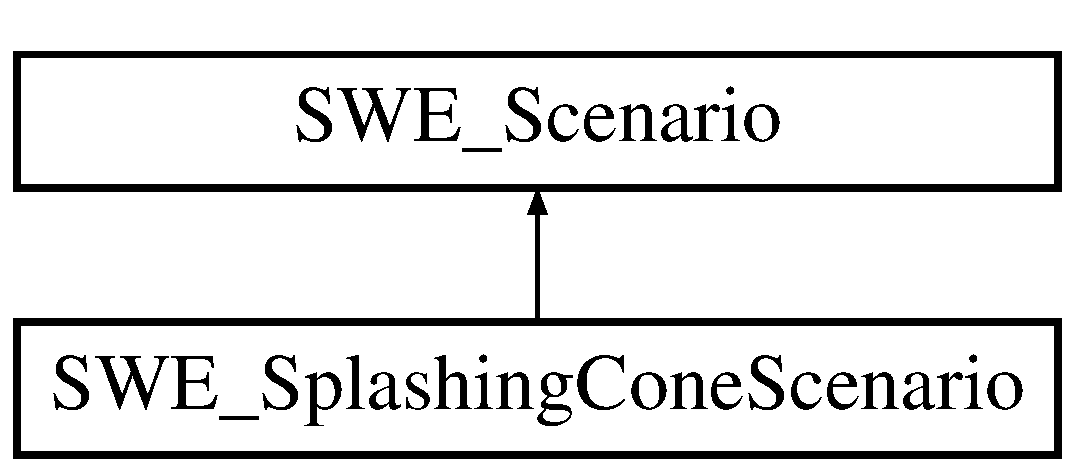
\includegraphics[height=2.000000cm]{classSWE__SplashingConeScenario}
\end{center}
\end{figure}
\subsection*{Public Member Functions}
\begin{DoxyCompactItemize}
\item 
float {\bfseries get\-Water\-Height} (float x, float y)\label{classSWE__SplashingConeScenario_a63d7b91dbd7dce764b12ba76eae856b9}

\item 
float {\bfseries get\-Bathymetry} (float x, float y)\label{classSWE__SplashingConeScenario_a54dff1212b8261e89270f9ab10081cb1}

\item 
float {\bfseries water\-Height\-At\-Rest} ()\label{classSWE__SplashingConeScenario_a430b3220b49368a4d20b69d71c087604}

\item 
float {\bfseries end\-Simulation} ()\label{classSWE__SplashingConeScenario_a464b296fc1905efc2e86aba909cc5188}

\item 
virtual {\bf Boundary\-Type} {\bfseries get\-Boundary\-Type} ({\bf Boundary\-Edge} edge)\label{classSWE__SplashingConeScenario_a8b8353a1f1cd58d9f211ccb32e4f3b33}

\end{DoxyCompactItemize}


\subsection{Detailed Description}
Scenario \char`\"{}\-Splashing Cone\char`\"{}\-: bathymetry forms a circular cone intial water surface designed to form \char`\"{}sea at rest\char`\"{} but\-: elevated water region in the centre (similar to radial dam break) 

The documentation for this class was generated from the following file\-:\begin{DoxyCompactItemize}
\item 
src/scenarios/{\bf S\-W\-E\-\_\-simple\-\_\-scenarios.\-hh}\end{DoxyCompactItemize}

\section{S\-W\-E\-\_\-\-Splashing\-Pool\-Scenario Class Reference}
\label{classSWE__SplashingPoolScenario}\index{S\-W\-E\-\_\-\-Splashing\-Pool\-Scenario@{S\-W\-E\-\_\-\-Splashing\-Pool\-Scenario}}


{\ttfamily \#include $<$S\-W\-E\-\_\-simple\-\_\-scenarios.\-hh$>$}

Inheritance diagram for S\-W\-E\-\_\-\-Splashing\-Pool\-Scenario\-:\begin{figure}[H]
\begin{center}
\leavevmode
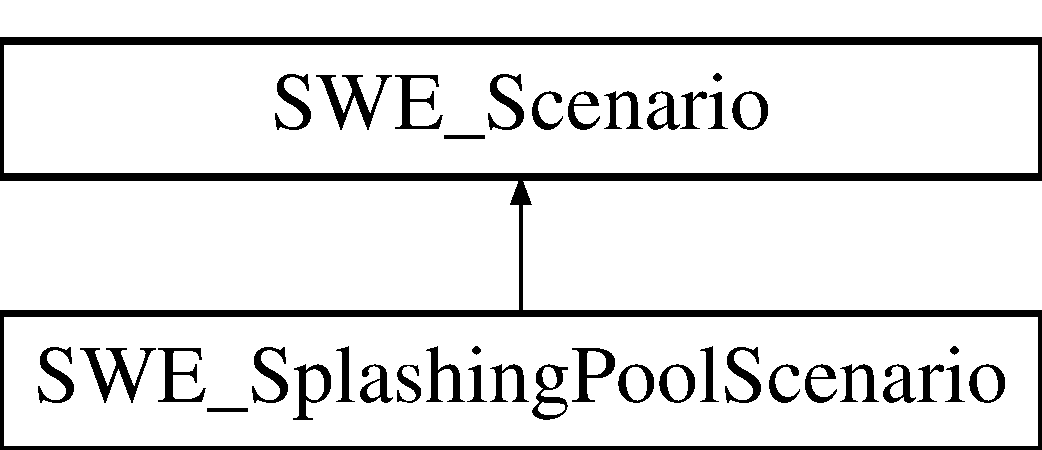
\includegraphics[height=2.000000cm]{classSWE__SplashingPoolScenario}
\end{center}
\end{figure}
\subsection*{Public Member Functions}
\begin{DoxyCompactItemize}
\item 
float {\bfseries get\-Bathymetry} (float x, float y)\label{classSWE__SplashingPoolScenario_a75c48073eb863d52fe38639ff0834e72}

\item 
float {\bfseries get\-Water\-Height} (float x, float y)\label{classSWE__SplashingPoolScenario_a45328d2cbff3068f6bde34d92dff0d1c}

\item 
virtual float {\bfseries end\-Simulation} ()\label{classSWE__SplashingPoolScenario_a49edaef6fbfad67c12f0ce1942e9f848}

\item 
float {\bf get\-Boundary\-Pos} ({\bf Boundary\-Edge} i\-\_\-edge)
\end{DoxyCompactItemize}


\subsection{Detailed Description}
Scenario \char`\"{}\-Splashing Pool\char`\"{}\-: intial water surface has a fixed slope (diagonal to x,y) 

\subsection{Member Function Documentation}
\index{S\-W\-E\-\_\-\-Splashing\-Pool\-Scenario@{S\-W\-E\-\_\-\-Splashing\-Pool\-Scenario}!get\-Boundary\-Pos@{get\-Boundary\-Pos}}
\index{get\-Boundary\-Pos@{get\-Boundary\-Pos}!SWE_SplashingPoolScenario@{S\-W\-E\-\_\-\-Splashing\-Pool\-Scenario}}
\subsubsection[{get\-Boundary\-Pos}]{\setlength{\rightskip}{0pt plus 5cm}float S\-W\-E\-\_\-\-Splashing\-Pool\-Scenario\-::get\-Boundary\-Pos (
\begin{DoxyParamCaption}
\item[{{\bf Boundary\-Edge}}]{i\-\_\-edge}
\end{DoxyParamCaption}
)\hspace{0.3cm}{\ttfamily [inline]}, {\ttfamily [virtual]}}\label{classSWE__SplashingPoolScenario_af9ca3bce236a98e2a7ee5165088c8ed6}
Get the boundary positions


\begin{DoxyParams}{Parameters}
{\em i\-\_\-edge} & which edge \\
\hline
\end{DoxyParams}
\begin{DoxyReturn}{Returns}
value in the corresponding dimension 
\end{DoxyReturn}


Reimplemented from {\bf S\-W\-E\-\_\-\-Scenario} \doxyref{}{p.}{classSWE__Scenario}.



The documentation for this class was generated from the following file\-:\begin{DoxyCompactItemize}
\item 
src/scenarios/{\bf S\-W\-E\-\_\-simple\-\_\-scenarios.\-hh}\end{DoxyCompactItemize}

\section{S\-W\-E\-\_\-\-Vis\-Info Class Reference}
\label{classSWE__VisInfo}\index{S\-W\-E\-\_\-\-Vis\-Info@{S\-W\-E\-\_\-\-Vis\-Info}}


{\ttfamily \#include $<$S\-W\-E\-\_\-\-Vis\-Info.\-hh$>$}

Inheritance diagram for S\-W\-E\-\_\-\-Vis\-Info\-:\begin{figure}[H]
\begin{center}
\leavevmode
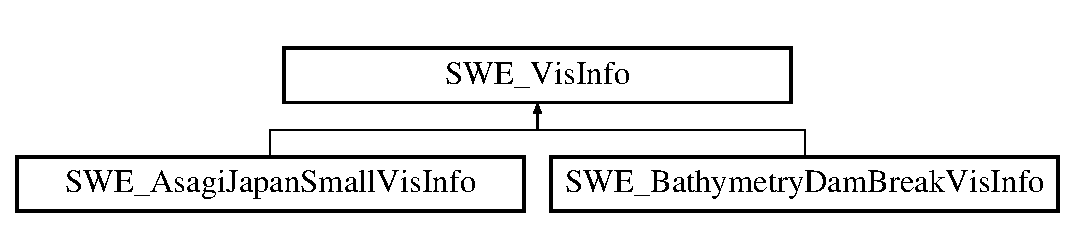
\includegraphics[height=2.000000cm]{classSWE__VisInfo}
\end{center}
\end{figure}
\subsection*{Public Member Functions}
\begin{DoxyCompactItemize}
\item 
virtual {\bf $\sim$\-S\-W\-E\-\_\-\-Vis\-Info} ()
\item 
virtual float {\bf water\-Vertical\-Scaling} ()
\item 
virtual float {\bf bathy\-Vertical\-Offset} ()
\item 
virtual float {\bf bathy\-Vertical\-Scaling} ()
\end{DoxyCompactItemize}


\subsection{Detailed Description}
\doxyref{S\-W\-E\-\_\-\-Vis\-Info}{p.}{classSWE__VisInfo} defines an interface that can be used for online visualization of a shallow water simulation. In particular, it provides information required for proper scaling of the involved variables.

For water height\-: displayed\-Water\-Height = \doxyref{water\-Vertical\-Scaling()}{p.}{classSWE__VisInfo_a9552a55a7581b7835d415315e2c17f04} $\ast$ simulated\-Water\-Height

For bathymetry\-: displayed\-Batyhmetry = \doxyref{bathy\-Vertical\-Scaling()}{p.}{classSWE__VisInfo_a10ddd7a192e67c69832e695e48b26e91} $\ast$ real\-Bathymetry
\begin{DoxyItemize}
\item \doxyref{bathy\-Vertical\-Offset()}{p.}{classSWE__VisInfo_a9c24e444c209f6f0c03a96950931e677}
\end{DoxyItemize}

The default water height should be 0. In this case a bathymetry value smaller than 0 means water and a value greater than 0 is land. Therefore bathy\-Vertical\-Offset should 0 for all real scenarios.

If you do not not provide an \doxyref{S\-W\-E\-\_\-\-Vis\-Info}{p.}{classSWE__VisInfo} for scenario, (water$\vert$bathy)Vertical\-Scaling will be guessed form the value initial values. bathy\-Vertical\-Offset is always 0 in this case. 

\subsection{Constructor \& Destructor Documentation}
\index{S\-W\-E\-\_\-\-Vis\-Info@{S\-W\-E\-\_\-\-Vis\-Info}!$\sim$\-S\-W\-E\-\_\-\-Vis\-Info@{$\sim$\-S\-W\-E\-\_\-\-Vis\-Info}}
\index{$\sim$\-S\-W\-E\-\_\-\-Vis\-Info@{$\sim$\-S\-W\-E\-\_\-\-Vis\-Info}!SWE_VisInfo@{S\-W\-E\-\_\-\-Vis\-Info}}
\subsubsection[{$\sim$\-S\-W\-E\-\_\-\-Vis\-Info}]{\setlength{\rightskip}{0pt plus 5cm}virtual S\-W\-E\-\_\-\-Vis\-Info\-::$\sim$\-S\-W\-E\-\_\-\-Vis\-Info (
\begin{DoxyParamCaption}
{}
\end{DoxyParamCaption}
)\hspace{0.3cm}{\ttfamily [inline]}, {\ttfamily [virtual]}}\label{classSWE__VisInfo_a40c49045acf4e50dc29551d767f11e15}
Empty virtual destructor 

\subsection{Member Function Documentation}
\index{S\-W\-E\-\_\-\-Vis\-Info@{S\-W\-E\-\_\-\-Vis\-Info}!bathy\-Vertical\-Offset@{bathy\-Vertical\-Offset}}
\index{bathy\-Vertical\-Offset@{bathy\-Vertical\-Offset}!SWE_VisInfo@{S\-W\-E\-\_\-\-Vis\-Info}}
\subsubsection[{bathy\-Vertical\-Offset}]{\setlength{\rightskip}{0pt plus 5cm}virtual float S\-W\-E\-\_\-\-Vis\-Info\-::bathy\-Vertical\-Offset (
\begin{DoxyParamCaption}
{}
\end{DoxyParamCaption}
)\hspace{0.3cm}{\ttfamily [inline]}, {\ttfamily [virtual]}}\label{classSWE__VisInfo_a9c24e444c209f6f0c03a96950931e677}
\begin{DoxyReturn}{Returns}
The vertical offset for the bathymetry. Should be 0 for \char`\"{}real\char`\"{} scenarios (scenarios with dry areas) 
\end{DoxyReturn}


Reimplemented in {\bf S\-W\-E\-\_\-\-Bathymetry\-Dam\-Break\-Vis\-Info} \doxyref{}{p.}{classSWE__BathymetryDamBreakVisInfo_aaecf007665b780a6066485ea0d2d2695}.

\index{S\-W\-E\-\_\-\-Vis\-Info@{S\-W\-E\-\_\-\-Vis\-Info}!bathy\-Vertical\-Scaling@{bathy\-Vertical\-Scaling}}
\index{bathy\-Vertical\-Scaling@{bathy\-Vertical\-Scaling}!SWE_VisInfo@{S\-W\-E\-\_\-\-Vis\-Info}}
\subsubsection[{bathy\-Vertical\-Scaling}]{\setlength{\rightskip}{0pt plus 5cm}virtual float S\-W\-E\-\_\-\-Vis\-Info\-::bathy\-Vertical\-Scaling (
\begin{DoxyParamCaption}
{}
\end{DoxyParamCaption}
)\hspace{0.3cm}{\ttfamily [inline]}, {\ttfamily [virtual]}}\label{classSWE__VisInfo_a10ddd7a192e67c69832e695e48b26e91}
\begin{DoxyReturn}{Returns}
The vertical scaling factor for the bathymetry 
\end{DoxyReturn}


Reimplemented in {\bf S\-W\-E\-\_\-\-Asagi\-Japan\-Small\-Vis\-Info} \doxyref{}{p.}{classSWE__AsagiJapanSmallVisInfo_ab25d85575460a76d88b90e2c927d49ac}.

\index{S\-W\-E\-\_\-\-Vis\-Info@{S\-W\-E\-\_\-\-Vis\-Info}!water\-Vertical\-Scaling@{water\-Vertical\-Scaling}}
\index{water\-Vertical\-Scaling@{water\-Vertical\-Scaling}!SWE_VisInfo@{S\-W\-E\-\_\-\-Vis\-Info}}
\subsubsection[{water\-Vertical\-Scaling}]{\setlength{\rightskip}{0pt plus 5cm}virtual float S\-W\-E\-\_\-\-Vis\-Info\-::water\-Vertical\-Scaling (
\begin{DoxyParamCaption}
{}
\end{DoxyParamCaption}
)\hspace{0.3cm}{\ttfamily [inline]}, {\ttfamily [virtual]}}\label{classSWE__VisInfo_a9552a55a7581b7835d415315e2c17f04}
\begin{DoxyReturn}{Returns}
The vertical scaling factor of the water 
\end{DoxyReturn}


Reimplemented in {\bf S\-W\-E\-\_\-\-Asagi\-Japan\-Small\-Vis\-Info} \doxyref{}{p.}{classSWE__AsagiJapanSmallVisInfo_a9c2092b5e02596e5ca2ba57c39d3b77e}.



The documentation for this class was generated from the following file\-:\begin{DoxyCompactItemize}
\item 
src/scenarios/{\bf S\-W\-E\-\_\-\-Vis\-Info.\-hh}\end{DoxyCompactItemize}

\section{S\-W\-E\-\_\-\-Wave\-Accumulation\-Block Class Reference}
\label{classSWE__WaveAccumulationBlock}\index{S\-W\-E\-\_\-\-Wave\-Accumulation\-Block@{S\-W\-E\-\_\-\-Wave\-Accumulation\-Block}}


{\ttfamily \#include $<$S\-W\-E\-\_\-\-Wave\-Accumulation\-Block.\-hh$>$}

Inheritance diagram for S\-W\-E\-\_\-\-Wave\-Accumulation\-Block\-:\begin{figure}[H]
\begin{center}
\leavevmode
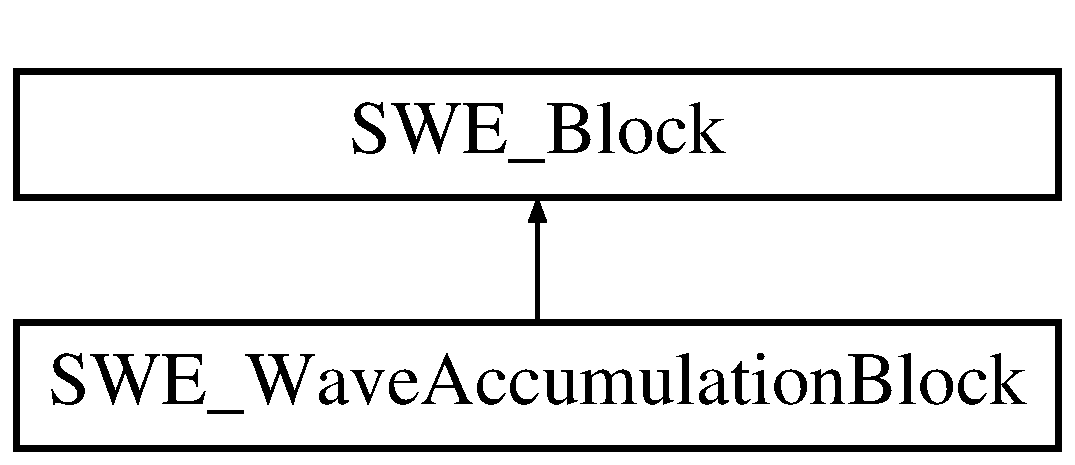
\includegraphics[height=2.000000cm]{classSWE__WaveAccumulationBlock}
\end{center}
\end{figure}
\subsection*{Public Member Functions}
\begin{DoxyCompactItemize}
\item 
{\bf S\-W\-E\-\_\-\-Wave\-Accumulation\-Block} (int l\-\_\-nx, int l\-\_\-ny, float l\-\_\-dx, float l\-\_\-dy)
\item 
void {\bf compute\-Numerical\-Fluxes} ()
\item 
void {\bf update\-Unknowns} (float dt)
\end{DoxyCompactItemize}
\subsection*{Additional Inherited Members}


\subsection{Detailed Description}
\doxyref{S\-W\-E\-\_\-\-Wave\-Accumulation\-Block}{p.}{classSWE__WaveAccumulationBlock} is an implementation of the \doxyref{S\-W\-E\-\_\-\-Block}{p.}{classSWE__Block} abstract class. It uses a wave propagation solver which is defined with the pre-\/compiler flag W\-A\-V\-E\-\_\-\-P\-R\-O\-P\-A\-G\-A\-T\-I\-O\-N\-\_\-\-S\-O\-L\-V\-E\-R (see above).

Possible wave propagation solvers are\-: F-\/\-Wave, Apprximate Augmented Riemann, Hybrid (f-\/wave + augmented). (details can be found in the corresponding source files) 

\subsection{Constructor \& Destructor Documentation}
\index{S\-W\-E\-\_\-\-Wave\-Accumulation\-Block@{S\-W\-E\-\_\-\-Wave\-Accumulation\-Block}!S\-W\-E\-\_\-\-Wave\-Accumulation\-Block@{S\-W\-E\-\_\-\-Wave\-Accumulation\-Block}}
\index{S\-W\-E\-\_\-\-Wave\-Accumulation\-Block@{S\-W\-E\-\_\-\-Wave\-Accumulation\-Block}!SWE_WaveAccumulationBlock@{S\-W\-E\-\_\-\-Wave\-Accumulation\-Block}}
\subsubsection[{S\-W\-E\-\_\-\-Wave\-Accumulation\-Block}]{\setlength{\rightskip}{0pt plus 5cm}S\-W\-E\-\_\-\-Wave\-Accumulation\-Block\-::\-S\-W\-E\-\_\-\-Wave\-Accumulation\-Block (
\begin{DoxyParamCaption}
\item[{int}]{l\-\_\-nx, }
\item[{int}]{l\-\_\-ny, }
\item[{float}]{l\-\_\-dx, }
\item[{float}]{l\-\_\-dy}
\end{DoxyParamCaption}
)}\label{classSWE__WaveAccumulationBlock_a20e04bf219dbf3d82c9f5eac1e7bd848}
Constructor of a \doxyref{S\-W\-E\-\_\-\-Wave\-Accumulation\-Block}{p.}{classSWE__WaveAccumulationBlock}.

Allocates the variables for the simulation\-: unknowns h,hu,hv,b are defined on grid indices [0,..,nx+1]$\ast$[0,..,ny+1] (-\/$>$ Abstract class \doxyref{S\-W\-E\-\_\-\-Block}{p.}{classSWE__Block}) -\/$>$ computational domain is [1,..,nx]$\ast$[1,..,ny] -\/$>$ plus ghost cell layer

Similar, all net-\/updates are defined as cell-\/local variables with indices [0,..,nx+1]$\ast$[0,..,ny+1], however, only values on [1,..,nx]$\ast$[1,..,ny] are used (i.\-e., ghost layers are not accessed). Net updates are intended to hold the accumulated(!) net updates computed on the edges. 

\subsection{Member Function Documentation}
\index{S\-W\-E\-\_\-\-Wave\-Accumulation\-Block@{S\-W\-E\-\_\-\-Wave\-Accumulation\-Block}!compute\-Numerical\-Fluxes@{compute\-Numerical\-Fluxes}}
\index{compute\-Numerical\-Fluxes@{compute\-Numerical\-Fluxes}!SWE_WaveAccumulationBlock@{S\-W\-E\-\_\-\-Wave\-Accumulation\-Block}}
\subsubsection[{compute\-Numerical\-Fluxes}]{\setlength{\rightskip}{0pt plus 5cm}void S\-W\-E\-\_\-\-Wave\-Accumulation\-Block\-::compute\-Numerical\-Fluxes (
\begin{DoxyParamCaption}
{}
\end{DoxyParamCaption}
)\hspace{0.3cm}{\ttfamily [virtual]}}\label{classSWE__WaveAccumulationBlock_acac0b73f22b256bc91a58ff8d0831e5d}
Compute net updates for the block. The member variable \doxyref{max\-Timestep}{p.}{classSWE__Block_a05cbc9b40e0483bf73dbc2bdeae7dee3} will be updated with the maximum allowed time step size 

Implements {\bf S\-W\-E\-\_\-\-Block} \doxyref{}{p.}{classSWE__Block_a94dcf2c6ae31731e4586e45628b0c00e}.

\index{S\-W\-E\-\_\-\-Wave\-Accumulation\-Block@{S\-W\-E\-\_\-\-Wave\-Accumulation\-Block}!update\-Unknowns@{update\-Unknowns}}
\index{update\-Unknowns@{update\-Unknowns}!SWE_WaveAccumulationBlock@{S\-W\-E\-\_\-\-Wave\-Accumulation\-Block}}
\subsubsection[{update\-Unknowns}]{\setlength{\rightskip}{0pt plus 5cm}void S\-W\-E\-\_\-\-Wave\-Accumulation\-Block\-::update\-Unknowns (
\begin{DoxyParamCaption}
\item[{float}]{dt}
\end{DoxyParamCaption}
)\hspace{0.3cm}{\ttfamily [virtual]}}\label{classSWE__WaveAccumulationBlock_a67b78723e81aec6e661b3710e6c41b43}
Updates the unknowns with the already computed net-\/updates.


\begin{DoxyParams}{Parameters}
{\em dt} & time step width used in the update. \\
\hline
\end{DoxyParams}


Implements {\bf S\-W\-E\-\_\-\-Block} \doxyref{}{p.}{classSWE__Block_ab2b4b659f23d5d45413dece8d2da3298}.



The documentation for this class was generated from the following files\-:\begin{DoxyCompactItemize}
\item 
src/blocks/{\bf S\-W\-E\-\_\-\-Wave\-Accumulation\-Block.\-hh}\item 
src/blocks/{\bf S\-W\-E\-\_\-\-Wave\-Accumulation\-Block.\-cpp}\end{DoxyCompactItemize}

\section{S\-W\-E\-\_\-\-Wave\-Propagation\-Block Class Reference}
\label{classSWE__WavePropagationBlock}\index{S\-W\-E\-\_\-\-Wave\-Propagation\-Block@{S\-W\-E\-\_\-\-Wave\-Propagation\-Block}}


{\ttfamily \#include $<$S\-W\-E\-\_\-\-Wave\-Propagation\-Block.\-hh$>$}

Inheritance diagram for S\-W\-E\-\_\-\-Wave\-Propagation\-Block\-:\begin{figure}[H]
\begin{center}
\leavevmode
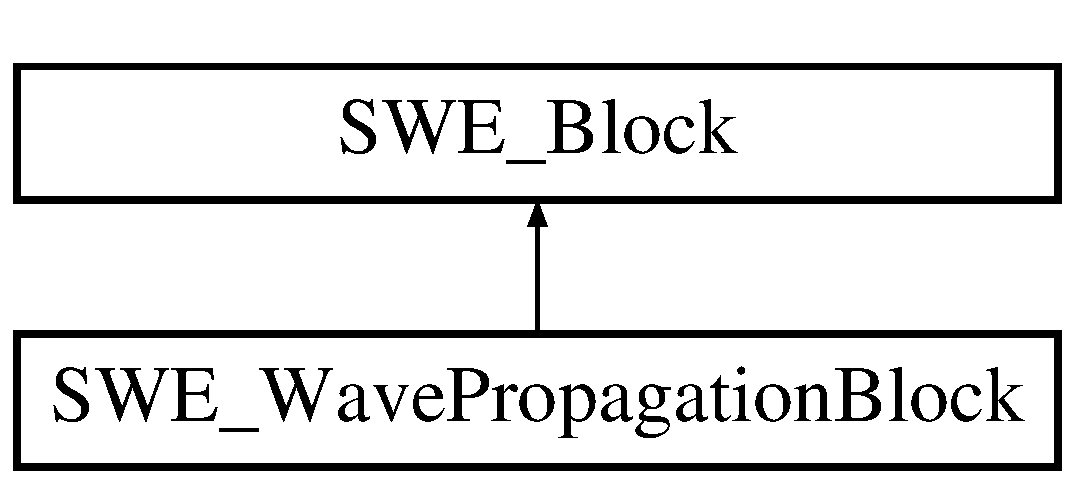
\includegraphics[height=2.000000cm]{classSWE__WavePropagationBlock}
\end{center}
\end{figure}
\subsection*{Public Member Functions}
\begin{DoxyCompactItemize}
\item 
{\bf S\-W\-E\-\_\-\-Wave\-Propagation\-Block} (int l\-\_\-nx, int l\-\_\-ny, float l\-\_\-dx, float l\-\_\-dy)
\item 
void {\bf compute\-Numerical\-Fluxes} ()
\item 
void {\bf update\-Unknowns} (float dt)
\item 
void {\bfseries update\-Unknowns\-Row} (float dt, int i)\label{classSWE__WavePropagationBlock_ad7c91177190b9d131387998d16fa7df6}

\item 
virtual {\bf $\sim$\-S\-W\-E\-\_\-\-Wave\-Propagation\-Block} ()
\end{DoxyCompactItemize}
\subsection*{Additional Inherited Members}


\subsection{Detailed Description}
\doxyref{S\-W\-E\-\_\-\-Wave\-Propagation\-Block}{p.}{classSWE__WavePropagationBlock} is an implementation of the \doxyref{S\-W\-E\-\_\-\-Block}{p.}{classSWE__Block} abstract class. It uses a wave propagation solver which is defined with the pre-\/compiler flag W\-A\-V\-E\-\_\-\-P\-R\-O\-P\-A\-G\-A\-T\-I\-O\-N\-\_\-\-S\-O\-L\-V\-E\-R (see above).

Possible wave propagation solvers are\-: F-\/\-Wave, Apprximate Augmented Riemann, Hybrid (f-\/wave + augmented). (details can be found in the corresponding source files) 

\subsection{Constructor \& Destructor Documentation}
\index{S\-W\-E\-\_\-\-Wave\-Propagation\-Block@{S\-W\-E\-\_\-\-Wave\-Propagation\-Block}!S\-W\-E\-\_\-\-Wave\-Propagation\-Block@{S\-W\-E\-\_\-\-Wave\-Propagation\-Block}}
\index{S\-W\-E\-\_\-\-Wave\-Propagation\-Block@{S\-W\-E\-\_\-\-Wave\-Propagation\-Block}!SWE_WavePropagationBlock@{S\-W\-E\-\_\-\-Wave\-Propagation\-Block}}
\subsubsection[{S\-W\-E\-\_\-\-Wave\-Propagation\-Block}]{\setlength{\rightskip}{0pt plus 5cm}S\-W\-E\-\_\-\-Wave\-Propagation\-Block\-::\-S\-W\-E\-\_\-\-Wave\-Propagation\-Block (
\begin{DoxyParamCaption}
\item[{int}]{l\-\_\-nx, }
\item[{int}]{l\-\_\-ny, }
\item[{float}]{l\-\_\-dx, }
\item[{float}]{l\-\_\-dy}
\end{DoxyParamCaption}
)}\label{classSWE__WavePropagationBlock_a9727e083d56a6d7aa9910f50c43080a9}
Constructor of a \doxyref{S\-W\-E\-\_\-\-Wave\-Propagation\-Block}{p.}{classSWE__WavePropagationBlock}.

Allocates the variables for the simulation\-: unknowns h,hu,hv,b are defined on grid indices [0,..,nx+1]$\ast$[0,..,ny+1] (-\/$>$ Abstract class \doxyref{S\-W\-E\-\_\-\-Block}{p.}{classSWE__Block}) -\/$>$ computational domain is [1,..,nx]$\ast$[1,..,ny] -\/$>$ plus ghost cell layer

net-\/updates are defined for edges with indices [0,..,nx]$\ast$[0,..,ny-\/1] or [0,..,nx-\/1]$\ast${\tt 0,..,ny}

A left/right net update with index (i-\/1,j-\/1) is located on the edge between cells with index (i-\/1,j) and (i,j)\-: 
\begin{DoxyPre}
  *********************
  *         *         *
  * (i-1,j) *  (i,j)  *
  *         *         *
  *********************\end{DoxyPre}



\begin{DoxyPre}            *
           ***
          *****
            *
            *
  NetUpdatesLeft(i-1,j-1)
            or
  NetUpdatesRight(i-1,j-1)
\end{DoxyPre}


A below/above net update with index (i-\/1, j-\/1) is located on the edge between cells with index (i, j-\/1) and (i,j)\-: 
\begin{DoxyPre}



  *         *
  * (i, j)  *   *
  *         *  **  NetUpdatesBelow(i-1,j-1)
  *********** *****         or
  *         *  **  NetUpdatesAbove(i-1,j-1)
  * (i,j-1) *   *
  *         *



\end{DoxyPre}
 \index{S\-W\-E\-\_\-\-Wave\-Propagation\-Block@{S\-W\-E\-\_\-\-Wave\-Propagation\-Block}!$\sim$\-S\-W\-E\-\_\-\-Wave\-Propagation\-Block@{$\sim$\-S\-W\-E\-\_\-\-Wave\-Propagation\-Block}}
\index{$\sim$\-S\-W\-E\-\_\-\-Wave\-Propagation\-Block@{$\sim$\-S\-W\-E\-\_\-\-Wave\-Propagation\-Block}!SWE_WavePropagationBlock@{S\-W\-E\-\_\-\-Wave\-Propagation\-Block}}
\subsubsection[{$\sim$\-S\-W\-E\-\_\-\-Wave\-Propagation\-Block}]{\setlength{\rightskip}{0pt plus 5cm}virtual S\-W\-E\-\_\-\-Wave\-Propagation\-Block\-::$\sim$\-S\-W\-E\-\_\-\-Wave\-Propagation\-Block (
\begin{DoxyParamCaption}
{}
\end{DoxyParamCaption}
)\hspace{0.3cm}{\ttfamily [inline]}, {\ttfamily [virtual]}}\label{classSWE__WavePropagationBlock_a9e53f3eaa7aee547ef88233069ff0667}
Destructor of a \doxyref{S\-W\-E\-\_\-\-Wave\-Propagation\-Block}{p.}{classSWE__WavePropagationBlock}.

In the case of a hybrid solver (N\-D\-E\-B\-U\-G not defined) information about the used solvers will be printed. 

\subsection{Member Function Documentation}
\index{S\-W\-E\-\_\-\-Wave\-Propagation\-Block@{S\-W\-E\-\_\-\-Wave\-Propagation\-Block}!compute\-Numerical\-Fluxes@{compute\-Numerical\-Fluxes}}
\index{compute\-Numerical\-Fluxes@{compute\-Numerical\-Fluxes}!SWE_WavePropagationBlock@{S\-W\-E\-\_\-\-Wave\-Propagation\-Block}}
\subsubsection[{compute\-Numerical\-Fluxes}]{\setlength{\rightskip}{0pt plus 5cm}void S\-W\-E\-\_\-\-Wave\-Propagation\-Block\-::compute\-Numerical\-Fluxes (
\begin{DoxyParamCaption}
{}
\end{DoxyParamCaption}
)\hspace{0.3cm}{\ttfamily [virtual]}}\label{classSWE__WavePropagationBlock_a5f6335a38fb3cf38623326959f06baf4}
Compute net updates for the block. The member variable \doxyref{max\-Timestep}{p.}{classSWE__Block_a05cbc9b40e0483bf73dbc2bdeae7dee3} will be updated with the maximum allowed time step size 

Implements {\bf S\-W\-E\-\_\-\-Block} \doxyref{}{p.}{classSWE__Block_a94dcf2c6ae31731e4586e45628b0c00e}.

\index{S\-W\-E\-\_\-\-Wave\-Propagation\-Block@{S\-W\-E\-\_\-\-Wave\-Propagation\-Block}!update\-Unknowns@{update\-Unknowns}}
\index{update\-Unknowns@{update\-Unknowns}!SWE_WavePropagationBlock@{S\-W\-E\-\_\-\-Wave\-Propagation\-Block}}
\subsubsection[{update\-Unknowns}]{\setlength{\rightskip}{0pt plus 5cm}void S\-W\-E\-\_\-\-Wave\-Propagation\-Block\-::update\-Unknowns (
\begin{DoxyParamCaption}
\item[{float}]{dt}
\end{DoxyParamCaption}
)\hspace{0.3cm}{\ttfamily [virtual]}}\label{classSWE__WavePropagationBlock_a1b1422472a36602b34180e4ed27f6d8c}
Updates the unknowns with the already computed net-\/updates.


\begin{DoxyParams}{Parameters}
{\em dt} & time step width used in the update. \\
\hline
\end{DoxyParams}


Implements {\bf S\-W\-E\-\_\-\-Block} \doxyref{}{p.}{classSWE__Block_ab2b4b659f23d5d45413dece8d2da3298}.



The documentation for this class was generated from the following files\-:\begin{DoxyCompactItemize}
\item 
src/blocks/{\bf S\-W\-E\-\_\-\-Wave\-Propagation\-Block.\-hh}\item 
src/blocks/{\bf S\-W\-E\-\_\-\-Wave\-Propagation\-Block.\-cpp}\end{DoxyCompactItemize}

\section{S\-W\-E\-\_\-\-Wave\-Propagation\-Block\-Cuda Class Reference}
\label{classSWE__WavePropagationBlockCuda}\index{S\-W\-E\-\_\-\-Wave\-Propagation\-Block\-Cuda@{S\-W\-E\-\_\-\-Wave\-Propagation\-Block\-Cuda}}


{\ttfamily \#include $<$S\-W\-E\-\_\-\-Wave\-Propagation\-Block\-Cuda.\-hh$>$}

Inheritance diagram for S\-W\-E\-\_\-\-Wave\-Propagation\-Block\-Cuda\-:\begin{figure}[H]
\begin{center}
\leavevmode
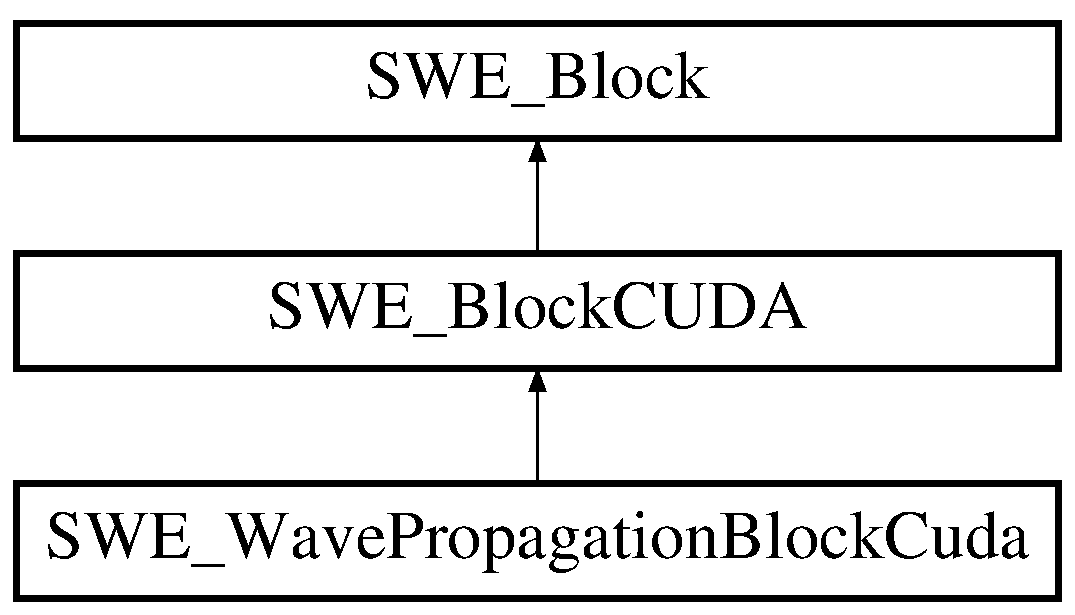
\includegraphics[height=3.000000cm]{classSWE__WavePropagationBlockCuda}
\end{center}
\end{figure}
\subsection*{Public Member Functions}
\begin{DoxyCompactItemize}
\item 
{\bfseries S\-W\-E\-\_\-\-Wave\-Propagation\-Block\-Cuda} (int l\-\_\-nx, int l\-\_\-ny, float l\-\_\-dx, float l\-\_\-dy)\label{classSWE__WavePropagationBlockCuda_a82f9de16ebab1bff58ead034416ab9ef}

\item 
void {\bf simulate\-Timestep} (float i\-\_\-d\-T)
\begin{DoxyCompactList}\small\item\em execute a single time step (with fixed time step size) of the simulation \end{DoxyCompactList}\item 
float {\bf simulate} (float, float)
\item 
void {\bf compute\-Numerical\-Fluxes} ()
\begin{DoxyCompactList}\small\item\em compute the numerical fluxes for each edge of the Cartesian grid \end{DoxyCompactList}\item 
void {\bf update\-Unknowns} (const float i\-\_\-delta\-T)
\begin{DoxyCompactList}\small\item\em compute the new values of the unknowns h, hu, and hv in all grid cells \end{DoxyCompactList}\end{DoxyCompactItemize}
\subsection*{Additional Inherited Members}


\subsection{Detailed Description}
\doxyref{S\-W\-E\-\_\-\-Wave\-Propagation\-Block\-Cuda}{p.}{classSWE__WavePropagationBlockCuda} is an implementation of the S\-W\-E\-\_\-\-Block\-Cuda abstract class. It uses a wave propagation solver which is defined with the pre-\/compiler flag W\-A\-V\-E\-\_\-\-P\-R\-O\-P\-A\-G\-A\-T\-I\-O\-N\-\_\-\-S\-O\-L\-V\-E\-R (see above).

Possible wave propagation solvers are\-: F-\/\-Wave, $<$strike$>$Approximate Augmented Riemann, Hybrid (f-\/wave + augmented).$<$/strike$>$ (details can be found in the corresponding source files) 

\subsection{Member Function Documentation}
\index{S\-W\-E\-\_\-\-Wave\-Propagation\-Block\-Cuda@{S\-W\-E\-\_\-\-Wave\-Propagation\-Block\-Cuda}!compute\-Numerical\-Fluxes@{compute\-Numerical\-Fluxes}}
\index{compute\-Numerical\-Fluxes@{compute\-Numerical\-Fluxes}!SWE_WavePropagationBlockCuda@{S\-W\-E\-\_\-\-Wave\-Propagation\-Block\-Cuda}}
\subsubsection[{compute\-Numerical\-Fluxes}]{\setlength{\rightskip}{0pt plus 5cm}void S\-W\-E\-\_\-\-Wave\-Propagation\-Block\-Cuda\-::compute\-Numerical\-Fluxes (
\begin{DoxyParamCaption}
{}
\end{DoxyParamCaption}
)\hspace{0.3cm}{\ttfamily [virtual]}}\label{classSWE__WavePropagationBlockCuda_a8a89bf61b9fc4433652f400ca8e564ed}


compute the numerical fluxes for each edge of the Cartesian grid 

The computation of fluxes strongly depends on the chosen numerical method. Hence, this purely virtual function has to be implemented in the respective derived classes. 

Implements {\bf S\-W\-E\-\_\-\-Block} \doxyref{}{p.}{classSWE__Block_a94dcf2c6ae31731e4586e45628b0c00e}.

\index{S\-W\-E\-\_\-\-Wave\-Propagation\-Block\-Cuda@{S\-W\-E\-\_\-\-Wave\-Propagation\-Block\-Cuda}!simulate@{simulate}}
\index{simulate@{simulate}!SWE_WavePropagationBlockCuda@{S\-W\-E\-\_\-\-Wave\-Propagation\-Block\-Cuda}}
\subsubsection[{simulate}]{\setlength{\rightskip}{0pt plus 5cm}float S\-W\-E\-\_\-\-Wave\-Propagation\-Block\-Cuda\-::simulate (
\begin{DoxyParamCaption}
\item[{float}]{i\-\_\-t\-Start, }
\item[{float}]{i\-\_\-t\-End}
\end{DoxyParamCaption}
)\hspace{0.3cm}{\ttfamily [virtual]}}\label{classSWE__WavePropagationBlockCuda_aa7cb155a2c8a76171fa39daff2b30ce3}
perform the simulation starting with simulation time t\-Start, until simulation time t\-End is reached

simulate implements the main simulation loop between two checkpoints; Note\-: this implementation can only be used, if you only use a single \doxyref{S\-W\-E\-\_\-\-Block}{p.}{classSWE__Block} and only apply simple boundary conditions! In particular, \doxyref{S\-W\-E\-\_\-\-Block\-::simulate}{p.}{classSWE__Block_a69784e2be2d09035fb2af9d306768f07} can not trigger calls to exchange values of copy and ghost layers between blocks! 
\begin{DoxyParams}{Parameters}
{\em t\-Start} & time where the simulation is started \\
\hline
{\em t\-End} & time of the next checkpoint \\
\hline
\end{DoxyParams}
\begin{DoxyReturn}{Returns}
actual end time reached 
\end{DoxyReturn}


Reimplemented from {\bf S\-W\-E\-\_\-\-Block} \doxyref{}{p.}{classSWE__Block_a69784e2be2d09035fb2af9d306768f07}.

\index{S\-W\-E\-\_\-\-Wave\-Propagation\-Block\-Cuda@{S\-W\-E\-\_\-\-Wave\-Propagation\-Block\-Cuda}!simulate\-Timestep@{simulate\-Timestep}}
\index{simulate\-Timestep@{simulate\-Timestep}!SWE_WavePropagationBlockCuda@{S\-W\-E\-\_\-\-Wave\-Propagation\-Block\-Cuda}}
\subsubsection[{simulate\-Timestep}]{\setlength{\rightskip}{0pt plus 5cm}void S\-W\-E\-\_\-\-Wave\-Propagation\-Block\-Cuda\-::simulate\-Timestep (
\begin{DoxyParamCaption}
\item[{float}]{dt}
\end{DoxyParamCaption}
)\hspace{0.3cm}{\ttfamily [virtual]}}\label{classSWE__WavePropagationBlockCuda_a1e79efd0b3f90e793add52fd5155410a}


execute a single time step (with fixed time step size) of the simulation 

Executes a single timestep with fixed time step size
\begin{DoxyItemize}
\item compute net updates for every edge
\item update cell values with the net updates
\end{DoxyItemize}


\begin{DoxyParams}{Parameters}
{\em dt} & time step width of the update \\
\hline
\end{DoxyParams}


Reimplemented from {\bf S\-W\-E\-\_\-\-Block} \doxyref{}{p.}{classSWE__Block_add6908e1ceb261a0a1f3ebc262cc5f11}.

\index{S\-W\-E\-\_\-\-Wave\-Propagation\-Block\-Cuda@{S\-W\-E\-\_\-\-Wave\-Propagation\-Block\-Cuda}!update\-Unknowns@{update\-Unknowns}}
\index{update\-Unknowns@{update\-Unknowns}!SWE_WavePropagationBlockCuda@{S\-W\-E\-\_\-\-Wave\-Propagation\-Block\-Cuda}}
\subsubsection[{update\-Unknowns}]{\setlength{\rightskip}{0pt plus 5cm}void S\-W\-E\-\_\-\-Wave\-Propagation\-Block\-Cuda\-::update\-Unknowns (
\begin{DoxyParamCaption}
\item[{const float}]{dt}
\end{DoxyParamCaption}
)\hspace{0.3cm}{\ttfamily [virtual]}}\label{classSWE__WavePropagationBlockCuda_a4163045a47a73515841e754ca3859fc5}


compute the new values of the unknowns h, hu, and hv in all grid cells 

based on the numerical fluxes (computed by compute\-Numerical\-Fluxes) and the specified time step size dt, an Euler time step is executed. As the computational fluxes will depend on the numerical method, this purely virtual function has to be implemented separately for each specific numerical model (and parallelisation approach). 
\begin{DoxyParams}{Parameters}
{\em dt} & size of the time step \\
\hline
\end{DoxyParams}


Implements {\bf S\-W\-E\-\_\-\-Block} \doxyref{}{p.}{classSWE__Block_ab2b4b659f23d5d45413dece8d2da3298}.



The documentation for this class was generated from the following file\-:\begin{DoxyCompactItemize}
\item 
src/blocks/cuda/{\bf S\-W\-E\-\_\-\-Wave\-Propagation\-Block\-Cuda.\-hh}\end{DoxyCompactItemize}

\section{S\-W\-E\-\_\-\-Wave\-Propagation\-Block\-S\-I\-M\-D Class Reference}
\label{classSWE__WavePropagationBlockSIMD}\index{S\-W\-E\-\_\-\-Wave\-Propagation\-Block\-S\-I\-M\-D@{S\-W\-E\-\_\-\-Wave\-Propagation\-Block\-S\-I\-M\-D}}


{\ttfamily \#include $<$S\-W\-E\-\_\-\-Wave\-Propagation\-Block\-S\-I\-M\-D.\-hh$>$}

Inheritance diagram for S\-W\-E\-\_\-\-Wave\-Propagation\-Block\-S\-I\-M\-D\-:\begin{figure}[H]
\begin{center}
\leavevmode
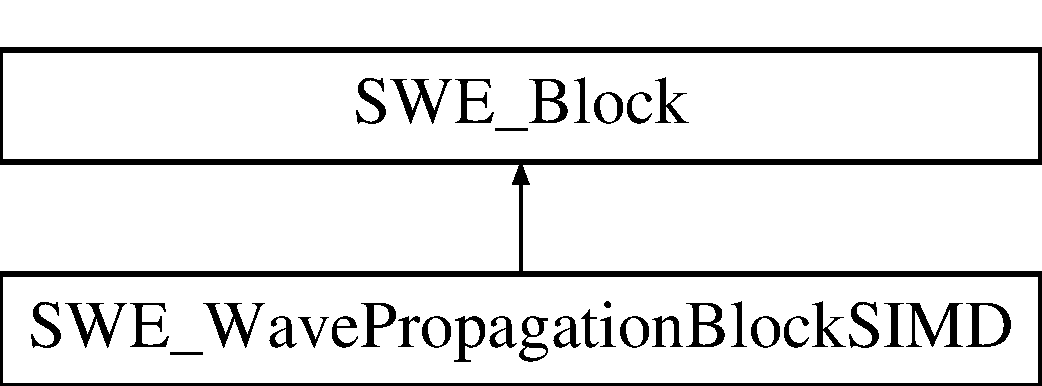
\includegraphics[height=2.000000cm]{classSWE__WavePropagationBlockSIMD}
\end{center}
\end{figure}
\subsection*{Public Member Functions}
\begin{DoxyCompactItemize}
\item 
{\bf S\-W\-E\-\_\-\-Wave\-Propagation\-Block\-S\-I\-M\-D} (int l\-\_\-nx, int l\-\_\-ny, float l\-\_\-dx, float l\-\_\-dy)
\item 
virtual void {\bf simulate\-Timestep} (float dt)
\item 
void {\bf compute\-Numerical\-Fluxes} ()
\item 
void {\bf update\-Unknowns} (float dt)
\item 
float {\bf simulate} (float i\-\_\-t\-Start, float i\-\_\-t\-End)
\item 
virtual {\bf $\sim$\-S\-W\-E\-\_\-\-Wave\-Propagation\-Block\-S\-I\-M\-D} ()
\end{DoxyCompactItemize}
\subsection*{Additional Inherited Members}


\subsection{Detailed Description}
\doxyref{S\-W\-E\-\_\-\-Wave\-Propagation\-Block\-S\-I\-M\-D}{p.}{classSWE__WavePropagationBlockSIMD} is an implementation of the \doxyref{S\-W\-E\-\_\-\-Block}{p.}{classSWE__Block} abstract class. It uses a wave propagation solver which is defined with the pre-\/compiler flag W\-A\-V\-E\-\_\-\-P\-R\-O\-P\-A\-G\-A\-T\-I\-O\-N\-\_\-\-S\-O\-L\-V\-E\-R (see above).

Possible wave propagation solvers are\-: F-\/\-Wave, Apprximate Augmented Riemann, Hybrid (f-\/wave + augmented). (details can be found in the corresponding source files) 

\subsection{Constructor \& Destructor Documentation}
\index{S\-W\-E\-\_\-\-Wave\-Propagation\-Block\-S\-I\-M\-D@{S\-W\-E\-\_\-\-Wave\-Propagation\-Block\-S\-I\-M\-D}!S\-W\-E\-\_\-\-Wave\-Propagation\-Block\-S\-I\-M\-D@{S\-W\-E\-\_\-\-Wave\-Propagation\-Block\-S\-I\-M\-D}}
\index{S\-W\-E\-\_\-\-Wave\-Propagation\-Block\-S\-I\-M\-D@{S\-W\-E\-\_\-\-Wave\-Propagation\-Block\-S\-I\-M\-D}!SWE_WavePropagationBlockSIMD@{S\-W\-E\-\_\-\-Wave\-Propagation\-Block\-S\-I\-M\-D}}
\subsubsection[{S\-W\-E\-\_\-\-Wave\-Propagation\-Block\-S\-I\-M\-D}]{\setlength{\rightskip}{0pt plus 5cm}S\-W\-E\-\_\-\-Wave\-Propagation\-Block\-S\-I\-M\-D\-::\-S\-W\-E\-\_\-\-Wave\-Propagation\-Block\-S\-I\-M\-D (
\begin{DoxyParamCaption}
\item[{int}]{l\-\_\-nx, }
\item[{int}]{l\-\_\-ny, }
\item[{float}]{l\-\_\-dx, }
\item[{float}]{l\-\_\-dy}
\end{DoxyParamCaption}
)}\label{classSWE__WavePropagationBlockSIMD_a57dc616f1aa84f33a9c75ecb116b3228}
Constructor of a \doxyref{S\-W\-E\-\_\-\-Wave\-Propagation\-Block\-S\-I\-M\-D}{p.}{classSWE__WavePropagationBlockSIMD}.

Allocates the variables for the simulation\-: unknowns h,hu,hv,b are defined on grid indices [0,..,nx+1]$\ast$[0,..,ny+1] (-\/$>$ Abstract class \doxyref{S\-W\-E\-\_\-\-Block}{p.}{classSWE__Block}) -\/$>$ computational domain is [1,..,nx]$\ast$[1,..,ny] -\/$>$ plus ghost cell layer

net-\/updates are defined for edges with indices [0,..,nx]$\ast$[0,..,ny-\/1] or [0,..,nx-\/1]$\ast${\tt 0,..,ny}

A left/right net update with index (i-\/1,j-\/1) is located on the edge between cells with index (i-\/1,j) and (i,j)\-: 
\begin{DoxyPre}
  *********************
  *         *         *
  * (i-1,j) *  (i,j)  *
  *         *         *
  *********************\end{DoxyPre}



\begin{DoxyPre}            *
           ***
          *****
            *
            *
  NetUpdatesLeft(i-1,j-1)
            or
  NetUpdatesRight(i-1,j-1)
\end{DoxyPre}


A below/above net update with index (i-\/1, j-\/1) is located on the edge between cells with index (i, j-\/1) and (i,j)\-: 
\begin{DoxyPre}



  *         *
  * (i, j)  *   *
  *         *  **  NetUpdatesBelow(i-1,j-1)
  *********** *****         or
  *         *  **  NetUpdatesAbove(i-1,j-1)
  * (i,j-1) *   *
  *         *



\end{DoxyPre}
 \index{S\-W\-E\-\_\-\-Wave\-Propagation\-Block\-S\-I\-M\-D@{S\-W\-E\-\_\-\-Wave\-Propagation\-Block\-S\-I\-M\-D}!$\sim$\-S\-W\-E\-\_\-\-Wave\-Propagation\-Block\-S\-I\-M\-D@{$\sim$\-S\-W\-E\-\_\-\-Wave\-Propagation\-Block\-S\-I\-M\-D}}
\index{$\sim$\-S\-W\-E\-\_\-\-Wave\-Propagation\-Block\-S\-I\-M\-D@{$\sim$\-S\-W\-E\-\_\-\-Wave\-Propagation\-Block\-S\-I\-M\-D}!SWE_WavePropagationBlockSIMD@{S\-W\-E\-\_\-\-Wave\-Propagation\-Block\-S\-I\-M\-D}}
\subsubsection[{$\sim$\-S\-W\-E\-\_\-\-Wave\-Propagation\-Block\-S\-I\-M\-D}]{\setlength{\rightskip}{0pt plus 5cm}virtual S\-W\-E\-\_\-\-Wave\-Propagation\-Block\-S\-I\-M\-D\-::$\sim$\-S\-W\-E\-\_\-\-Wave\-Propagation\-Block\-S\-I\-M\-D (
\begin{DoxyParamCaption}
{}
\end{DoxyParamCaption}
)\hspace{0.3cm}{\ttfamily [inline]}, {\ttfamily [virtual]}}\label{classSWE__WavePropagationBlockSIMD_aee73625ee731614849f398ea392137a7}
Destructor of a \doxyref{S\-W\-E\-\_\-\-Wave\-Propagation\-Block\-S\-I\-M\-D}{p.}{classSWE__WavePropagationBlockSIMD}.

In the case of a hybrid solver (N\-D\-E\-B\-U\-G not defined) information about the used solvers will be printed. 

\subsection{Member Function Documentation}
\index{S\-W\-E\-\_\-\-Wave\-Propagation\-Block\-S\-I\-M\-D@{S\-W\-E\-\_\-\-Wave\-Propagation\-Block\-S\-I\-M\-D}!compute\-Numerical\-Fluxes@{compute\-Numerical\-Fluxes}}
\index{compute\-Numerical\-Fluxes@{compute\-Numerical\-Fluxes}!SWE_WavePropagationBlockSIMD@{S\-W\-E\-\_\-\-Wave\-Propagation\-Block\-S\-I\-M\-D}}
\subsubsection[{compute\-Numerical\-Fluxes}]{\setlength{\rightskip}{0pt plus 5cm}void S\-W\-E\-\_\-\-Wave\-Propagation\-Block\-S\-I\-M\-D\-::compute\-Numerical\-Fluxes (
\begin{DoxyParamCaption}
{}
\end{DoxyParamCaption}
)\hspace{0.3cm}{\ttfamily [virtual]}}\label{classSWE__WavePropagationBlockSIMD_a4aa15050ec1db113f54fff06539a900f}
Compute net updates for the block. The member variable \doxyref{max\-Timestep}{p.}{classSWE__Block_a05cbc9b40e0483bf73dbc2bdeae7dee3} will be updated with the maximum allowed time step size 

Implements {\bf S\-W\-E\-\_\-\-Block} \doxyref{}{p.}{classSWE__Block_a94dcf2c6ae31731e4586e45628b0c00e}.

\index{S\-W\-E\-\_\-\-Wave\-Propagation\-Block\-S\-I\-M\-D@{S\-W\-E\-\_\-\-Wave\-Propagation\-Block\-S\-I\-M\-D}!simulate@{simulate}}
\index{simulate@{simulate}!SWE_WavePropagationBlockSIMD@{S\-W\-E\-\_\-\-Wave\-Propagation\-Block\-S\-I\-M\-D}}
\subsubsection[{simulate}]{\setlength{\rightskip}{0pt plus 5cm}float S\-W\-E\-\_\-\-Wave\-Propagation\-Block\-S\-I\-M\-D\-::simulate (
\begin{DoxyParamCaption}
\item[{float}]{i\-\_\-t\-Start, }
\item[{float}]{i\-\_\-t\-End}
\end{DoxyParamCaption}
)\hspace{0.3cm}{\ttfamily [virtual]}}\label{classSWE__WavePropagationBlockSIMD_a6c54dbcd43a77b46bae4de36b8d16af7}
Runs the simulation until i\-\_\-t\-End is reached.


\begin{DoxyParams}{Parameters}
{\em i\-\_\-t\-Start} & time when the simulation starts \\
\hline
{\em i\-\_\-t\-End} & time when the simulation should end \\
\hline
\end{DoxyParams}
\begin{DoxyReturn}{Returns}
time we reached after the last update step, in general a bit later than i\-\_\-t\-End 
\end{DoxyReturn}


Reimplemented from {\bf S\-W\-E\-\_\-\-Block} \doxyref{}{p.}{classSWE__Block_a69784e2be2d09035fb2af9d306768f07}.

\index{S\-W\-E\-\_\-\-Wave\-Propagation\-Block\-S\-I\-M\-D@{S\-W\-E\-\_\-\-Wave\-Propagation\-Block\-S\-I\-M\-D}!simulate\-Timestep@{simulate\-Timestep}}
\index{simulate\-Timestep@{simulate\-Timestep}!SWE_WavePropagationBlockSIMD@{S\-W\-E\-\_\-\-Wave\-Propagation\-Block\-S\-I\-M\-D}}
\subsubsection[{simulate\-Timestep}]{\setlength{\rightskip}{0pt plus 5cm}void S\-W\-E\-\_\-\-Wave\-Propagation\-Block\-S\-I\-M\-D\-::simulate\-Timestep (
\begin{DoxyParamCaption}
\item[{float}]{dt}
\end{DoxyParamCaption}
)\hspace{0.3cm}{\ttfamily [virtual]}}\label{classSWE__WavePropagationBlockSIMD_a99c288632c402eaf7dff76f03624872a}
Update the bathymetry values with the displacement corresponding to the current time step.


\begin{DoxyParams}{Parameters}
{\em i\-\_\-asagi\-Scenario} & the corresponding A\-S\-A\-G\-I-\/scenario Executes a single timestep.
\begin{DoxyItemize}
\item compute net updates for every edge
\item update cell values with the net updates
\end{DoxyItemize}\\
\hline
{\em dt} & time step width of the update \\
\hline
\end{DoxyParams}


Reimplemented from {\bf S\-W\-E\-\_\-\-Block} \doxyref{}{p.}{classSWE__Block_add6908e1ceb261a0a1f3ebc262cc5f11}.

\index{S\-W\-E\-\_\-\-Wave\-Propagation\-Block\-S\-I\-M\-D@{S\-W\-E\-\_\-\-Wave\-Propagation\-Block\-S\-I\-M\-D}!update\-Unknowns@{update\-Unknowns}}
\index{update\-Unknowns@{update\-Unknowns}!SWE_WavePropagationBlockSIMD@{S\-W\-E\-\_\-\-Wave\-Propagation\-Block\-S\-I\-M\-D}}
\subsubsection[{update\-Unknowns}]{\setlength{\rightskip}{0pt plus 5cm}void S\-W\-E\-\_\-\-Wave\-Propagation\-Block\-S\-I\-M\-D\-::update\-Unknowns (
\begin{DoxyParamCaption}
\item[{float}]{dt}
\end{DoxyParamCaption}
)\hspace{0.3cm}{\ttfamily [virtual]}}\label{classSWE__WavePropagationBlockSIMD_a2596238868efd3cdd453d9ac2de15997}
Updates the unknowns with the already computed net-\/updates.


\begin{DoxyParams}{Parameters}
{\em dt} & time step width used in the update. \\
\hline
\end{DoxyParams}


Implements {\bf S\-W\-E\-\_\-\-Block} \doxyref{}{p.}{classSWE__Block_ab2b4b659f23d5d45413dece8d2da3298}.



The documentation for this class was generated from the following files\-:\begin{DoxyCompactItemize}
\item 
src/blocks/{\bf S\-W\-E\-\_\-\-Wave\-Propagation\-Block\-S\-I\-M\-D.\-hh}\item 
src/blocks/{\bf S\-W\-E\-\_\-\-Wave\-Propagation\-Block\-S\-I\-M\-D.\-cpp}\end{DoxyCompactItemize}

\section{Text Class Reference}
\label{classText}\index{Text@{Text}}
\subsection*{Public Member Functions}
\begin{DoxyCompactItemize}
\item 
void {\bfseries add\-Text} (const char $\ast$text)\label{classText_a26d2ab34aeb3b764b90221a473b4047f}

\item 
void {\bfseries start\-Text\-Mode} ()\label{classText_aff5cec718fcce7381d2d08717441af7f}

\item 
bool {\bf show\-Next\-Text} (S\-D\-L\-\_\-\-Rect \&location)
\item 
void {\bfseries end\-Text\-Mode} ()\label{classText_a8f046f44006bf0a973b83cdc0d218e29}

\end{DoxyCompactItemize}


\subsection{Member Function Documentation}
\index{Text@{Text}!show\-Next\-Text@{show\-Next\-Text}}
\index{show\-Next\-Text@{show\-Next\-Text}!Text@{Text}}
\subsubsection[{show\-Next\-Text}]{\setlength{\rightskip}{0pt plus 5cm}bool Text\-::show\-Next\-Text (
\begin{DoxyParamCaption}
\item[{S\-D\-L\-\_\-\-Rect \&}]{location}
\end{DoxyParamCaption}
)\hspace{0.3cm}{\ttfamily [inline]}}\label{classText_a45299ae1fa870add85abe5f587428759}
\begin{DoxyReturn}{Returns}
True there are more textures 
\end{DoxyReturn}


The documentation for this class was generated from the following files\-:\begin{DoxyCompactItemize}
\item 
src/opengl/text.\-h\item 
src/opengl/text.\-cpp\end{DoxyCompactItemize}

\section{V\-B\-O Class Reference}
\label{classVBO}\index{V\-B\-O@{V\-B\-O}}
\subsection*{Public Member Functions}
\begin{DoxyCompactItemize}
\item 
void {\bf init} ()
\item 
G\-Luint {\bf get\-Name} ()
\item 
void {\bfseries set\-Buffer\-Data} (G\-Lsizei size, const void $\ast$data, G\-Lenum target=G\-L\-\_\-\-A\-R\-R\-A\-Y\-\_\-\-B\-U\-F\-F\-E\-R, G\-Lenum usage=G\-L\-\_\-\-S\-T\-A\-T\-I\-C\-\_\-\-D\-R\-A\-W)\label{classVBO_a69960020a34122b6d4becdbf44ccdcd8}

\item 
void {\bfseries bind\-Buffer} (G\-Lenum target=G\-L\-\_\-\-A\-R\-R\-A\-Y\-\_\-\-B\-U\-F\-F\-E\-R)\label{classVBO_a3928672efb7ee07b0c5662e4dd7b421a}

\item 
void {\bf finialize} ()
\end{DoxyCompactItemize}


\subsection{Member Function Documentation}
\index{V\-B\-O@{V\-B\-O}!finialize@{finialize}}
\index{finialize@{finialize}!VBO@{V\-B\-O}}
\subsubsection[{finialize}]{\setlength{\rightskip}{0pt plus 5cm}void V\-B\-O\-::finialize (
\begin{DoxyParamCaption}
{}
\end{DoxyParamCaption}
)\hspace{0.3cm}{\ttfamily [inline]}}\label{classVBO_a82cfb6c197f276eca01c409f064bf26c}
Frees all associated memory \index{V\-B\-O@{V\-B\-O}!get\-Name@{get\-Name}}
\index{get\-Name@{get\-Name}!VBO@{V\-B\-O}}
\subsubsection[{get\-Name}]{\setlength{\rightskip}{0pt plus 5cm}G\-Luint V\-B\-O\-::get\-Name (
\begin{DoxyParamCaption}
{}
\end{DoxyParamCaption}
)\hspace{0.3cm}{\ttfamily [inline]}}\label{classVBO_affdb3a55d47548b939aad6a166af9310}
\begin{DoxyReturn}{Returns}
The Open\-G\-L name of the buffer 
\end{DoxyReturn}
\index{V\-B\-O@{V\-B\-O}!init@{init}}
\index{init@{init}!VBO@{V\-B\-O}}
\subsubsection[{init}]{\setlength{\rightskip}{0pt plus 5cm}void V\-B\-O\-::init (
\begin{DoxyParamCaption}
{}
\end{DoxyParamCaption}
)}\label{classVBO_af1a4a8c60cac7e02e371db3d9fe496a4}
Initializes the object 

The documentation for this class was generated from the following files\-:\begin{DoxyCompactItemize}
\item 
src/opengl/{\bf vbo.\-h}\item 
src/opengl/{\bf vbo.\-cpp}\end{DoxyCompactItemize}

\section{Visualization Class Reference}
\label{classVisualization}\index{Visualization@{Visualization}}
\subsection*{Public Member Functions}
\begin{DoxyCompactItemize}
\item 
{\bf Visualization} (int window\-Width, int window\-Height, const char $\ast$window\-\_\-title)
\item 
{\bf $\sim$\-Visualization} ()
\item 
void {\bf init} ({\bf Simulation} \&sim, {\bf S\-W\-E\-\_\-\-Vis\-Info} $\ast$vis\-Info=0\-L)
\item 
void {\bf clean\-Up} ()
\item 
cuda\-Graphics\-Resource $\ast$$\ast$ {\bf get\-Cuda\-Normals\-Ptr} ()
\item 
cuda\-Graphics\-Resource $\ast$$\ast$ {\bf get\-Cuda\-Water\-Surface\-Ptr} ()
\item 
void {\bf render\-Display} ()
\item 
void {\bfseries modify\-Water\-Scaling} (float factor)\label{classVisualization_a8c985ef294e7d35ab65257c30f757807}

\item 
void {\bf set\-Rendering\-Mode} (Render\-Mode mode)
\item 
void {\bf toggle\-Rendering\-Mode} ()
\item 
int {\bf resize\-Window} (int new\-Width, int new\-Height)
\end{DoxyCompactItemize}
\subsection*{Static Public Member Functions}
\begin{DoxyCompactItemize}
\item 
static bool {\bf is\-Extension\-Supported} (const char $\ast$sz\-Target\-Extension)
\end{DoxyCompactItemize}
\subsection*{Public Attributes}
\begin{DoxyCompactItemize}
\item 
{\bf Camera} $\ast$ {\bfseries camera}\label{classVisualization_a7013e42778d25e78c1d45724895b8442}

\end{DoxyCompactItemize}


\subsection{Constructor \& Destructor Documentation}
\index{Visualization@{Visualization}!Visualization@{Visualization}}
\index{Visualization@{Visualization}!Visualization@{Visualization}}
\subsubsection[{Visualization}]{\setlength{\rightskip}{0pt plus 5cm}Visualization\-::\-Visualization (
\begin{DoxyParamCaption}
\item[{int}]{window\-Width, }
\item[{int}]{window\-Height, }
\item[{const char $\ast$}]{window\-\_\-title}
\end{DoxyParamCaption}
)}\label{classVisualization_af3e258903a7c4b52a12cfbeb3332aed8}
Constructor. All dimensions are node-\/based, this means a grid consisting of 2x2 cells would have 3x3 nodes.


\begin{DoxyParams}{Parameters}
{\em } & window\-\_\-title title of the window created \\
\hline
{\em } & \-\_\-grid\-\_\-x\-\_\-size number of nodes of the grid (in x-\/direction) \\
\hline
{\em } & \-\_\-grid\-\_\-y\-\_\-size number of nodes of the grid (in y-\/direction) \\
\hline
\end{DoxyParams}
\index{Visualization@{Visualization}!$\sim$\-Visualization@{$\sim$\-Visualization}}
\index{$\sim$\-Visualization@{$\sim$\-Visualization}!Visualization@{Visualization}}
\subsubsection[{$\sim$\-Visualization}]{\setlength{\rightskip}{0pt plus 5cm}Visualization\-::$\sim$\-Visualization (
\begin{DoxyParamCaption}
{}
\end{DoxyParamCaption}
)}\label{classVisualization_a1b3dc8c07a781aaf8f4cbe95031e191c}
Destructor (see note below) 

\subsection{Member Function Documentation}
\index{Visualization@{Visualization}!clean\-Up@{clean\-Up}}
\index{clean\-Up@{clean\-Up}!Visualization@{Visualization}}
\subsubsection[{clean\-Up}]{\setlength{\rightskip}{0pt plus 5cm}void Visualization\-::clean\-Up (
\begin{DoxyParamCaption}
{}
\end{DoxyParamCaption}
)}\label{classVisualization_a9f636583bc52bd7b5180eff2751fbb70}
Frees all memory we used for geometry data Needs to be called before destructor gets called in order to work correctly \index{Visualization@{Visualization}!get\-Cuda\-Normals\-Ptr@{get\-Cuda\-Normals\-Ptr}}
\index{get\-Cuda\-Normals\-Ptr@{get\-Cuda\-Normals\-Ptr}!Visualization@{Visualization}}
\subsubsection[{get\-Cuda\-Normals\-Ptr}]{\setlength{\rightskip}{0pt plus 5cm}cuda\-Graphics\-Resource $\ast$$\ast$ Visualization\-::get\-Cuda\-Normals\-Ptr (
\begin{DoxyParamCaption}
{}
\end{DoxyParamCaption}
)}\label{classVisualization_a0c618934d4dc368e4f400099c9aa2e84}
Returns a pointer to the cuda memory object holding the vertex normals \index{Visualization@{Visualization}!get\-Cuda\-Water\-Surface\-Ptr@{get\-Cuda\-Water\-Surface\-Ptr}}
\index{get\-Cuda\-Water\-Surface\-Ptr@{get\-Cuda\-Water\-Surface\-Ptr}!Visualization@{Visualization}}
\subsubsection[{get\-Cuda\-Water\-Surface\-Ptr}]{\setlength{\rightskip}{0pt plus 5cm}cuda\-Graphics\-Resource $\ast$$\ast$ Visualization\-::get\-Cuda\-Water\-Surface\-Ptr (
\begin{DoxyParamCaption}
{}
\end{DoxyParamCaption}
)}\label{classVisualization_aa19e824f46baf01a66b1d991107f26f2}
Returns a pointer to the cuda memory object holding the vertex positions \index{Visualization@{Visualization}!init@{init}}
\index{init@{init}!Visualization@{Visualization}}
\subsubsection[{init}]{\setlength{\rightskip}{0pt plus 5cm}void Visualization\-::init (
\begin{DoxyParamCaption}
\item[{{\bf Simulation} \&}]{sim, }
\item[{{\bf S\-W\-E\-\_\-\-Vis\-Info} $\ast$}]{vis\-Info = {\ttfamily 0L}}
\end{DoxyParamCaption}
)}\label{classVisualization_ad2ba8e6ef021127f111419c6c2605842}
Allocates memory for vertices and other geometry data.


\begin{DoxyParams}{Parameters}
{\em sim} & instance of the simulation class \\
\hline
\end{DoxyParams}
\index{Visualization@{Visualization}!is\-Extension\-Supported@{is\-Extension\-Supported}}
\index{is\-Extension\-Supported@{is\-Extension\-Supported}!Visualization@{Visualization}}
\subsubsection[{is\-Extension\-Supported}]{\setlength{\rightskip}{0pt plus 5cm}bool Visualization\-::is\-Extension\-Supported (
\begin{DoxyParamCaption}
\item[{const char $\ast$}]{sz\-Target\-Extension}
\end{DoxyParamCaption}
)\hspace{0.3cm}{\ttfamily [static]}}\label{classVisualization_a4d2ba4c344b5c6aca5410123281ddbc9}
Returns, whether a special extension is supported by the current graphics card


\begin{DoxyParams}{Parameters}
{\em sz\-Target\-Extention} & string describing the extension to look for \\
\hline
\end{DoxyParams}
\index{Visualization@{Visualization}!render\-Display@{render\-Display}}
\index{render\-Display@{render\-Display}!Visualization@{Visualization}}
\subsubsection[{render\-Display}]{\setlength{\rightskip}{0pt plus 5cm}void Visualization\-::render\-Display (
\begin{DoxyParamCaption}
{}
\end{DoxyParamCaption}
)}\label{classVisualization_acce7d4076eb313acaa526741428b53cb}
Main rendering function. Draws the scene and updates screen \index{Visualization@{Visualization}!resize\-Window@{resize\-Window}}
\index{resize\-Window@{resize\-Window}!Visualization@{Visualization}}
\subsubsection[{resize\-Window}]{\setlength{\rightskip}{0pt plus 5cm}int Visualization\-::resize\-Window (
\begin{DoxyParamCaption}
\item[{int}]{new\-Width, }
\item[{int}]{new\-Height}
\end{DoxyParamCaption}
)}\label{classVisualization_a0bb75d211b64d94fddf5e17b80c3f165}
Gets called when window gets resized


\begin{DoxyParams}{Parameters}
{\em new\-Width} & new window width in pixels \\
\hline
{\em new\-Height} & height in pixels \\
\hline
\end{DoxyParams}
\index{Visualization@{Visualization}!set\-Rendering\-Mode@{set\-Rendering\-Mode}}
\index{set\-Rendering\-Mode@{set\-Rendering\-Mode}!Visualization@{Visualization}}
\subsubsection[{set\-Rendering\-Mode}]{\setlength{\rightskip}{0pt plus 5cm}void Visualization\-::set\-Rendering\-Mode (
\begin{DoxyParamCaption}
\item[{Render\-Mode}]{mode}
\end{DoxyParamCaption}
)}\label{classVisualization_ae608b97c9e82e78b212cc1cb2b744c5d}
Sets current rendering mode


\begin{DoxyParams}{Parameters}
{\em mode} & rendering mode \\
\hline
\end{DoxyParams}
\index{Visualization@{Visualization}!toggle\-Rendering\-Mode@{toggle\-Rendering\-Mode}}
\index{toggle\-Rendering\-Mode@{toggle\-Rendering\-Mode}!Visualization@{Visualization}}
\subsubsection[{toggle\-Rendering\-Mode}]{\setlength{\rightskip}{0pt plus 5cm}void Visualization\-::toggle\-Rendering\-Mode (
\begin{DoxyParamCaption}
{}
\end{DoxyParamCaption}
)}\label{classVisualization_a39038b57b96b4718c2c06710100d6317}
Switches between 3 different rendering modes\-:
\begin{DoxyItemize}
\item Shaded\-: Use Open\-G\-L shading
\item Wireframe\-: Only render edges of each triangle
\item Watershader\-: Use custom G\-L\-S\-L shader for water surface 
\end{DoxyItemize}

The documentation for this class was generated from the following files\-:\begin{DoxyCompactItemize}
\item 
src/opengl/visualization.\-h\item 
src/opengl/visualization.\-cpp\end{DoxyCompactItemize}

\section{io\-:\-:Vtk\-Writer Class Reference}
\label{classio_1_1VtkWriter}\index{io\-::\-Vtk\-Writer@{io\-::\-Vtk\-Writer}}
Inheritance diagram for io\-:\-:Vtk\-Writer\-:\begin{figure}[H]
\begin{center}
\leavevmode
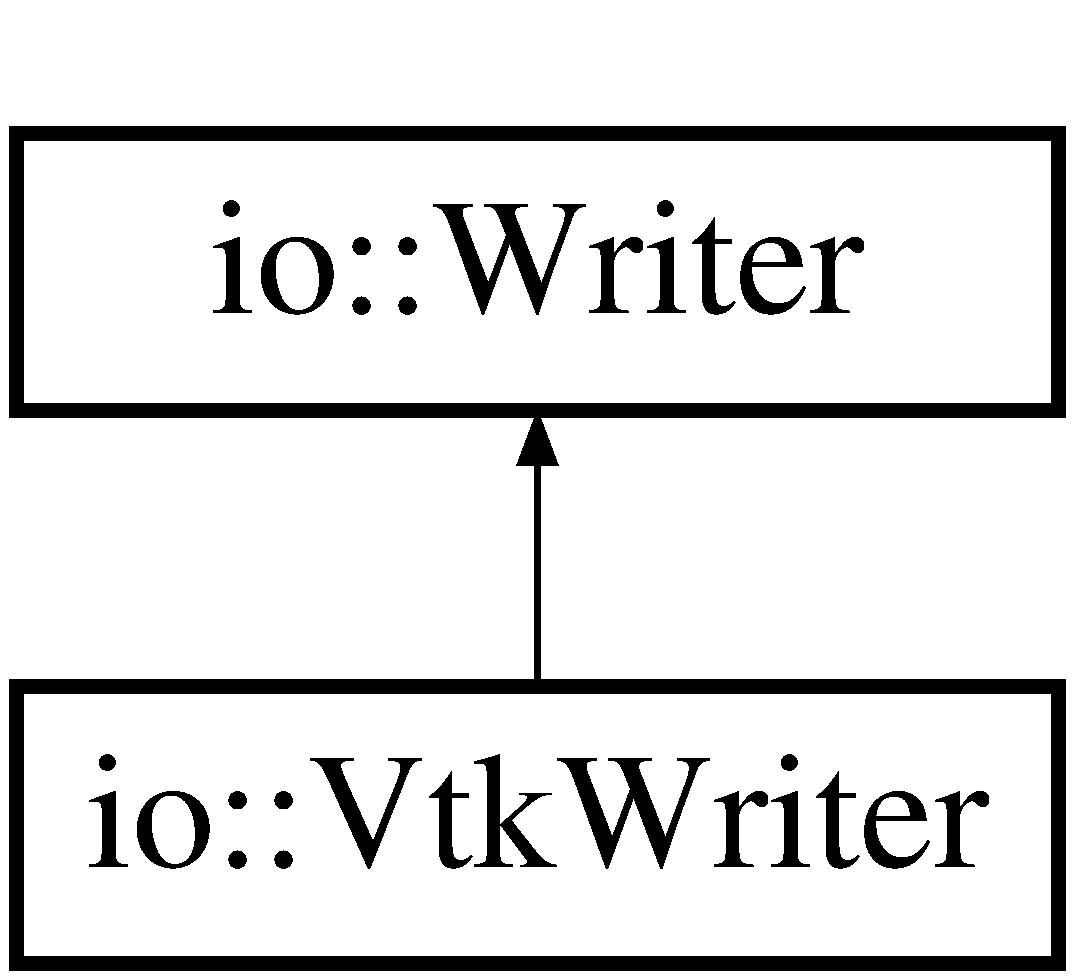
\includegraphics[height=2.000000cm]{classio_1_1VtkWriter}
\end{center}
\end{figure}
\subsection*{Public Member Functions}
\begin{DoxyCompactItemize}
\item 
{\bf Vtk\-Writer} (const std\-::string \&i\-\_\-file\-Name, const {\bf Float2\-D} \&i\-\_\-b, const {\bf Boundary\-Size} \&i\-\_\-boundary\-Size, int i\-\_\-n\-X, int i\-\_\-n\-Y, float i\-\_\-d\-X, float i\-\_\-d\-Y, int i\-\_\-offset\-X=0, int i\-\_\-offset\-Y=0)
\item 
void {\bf write\-Time\-Step} (const {\bf Float2\-D} \&i\-\_\-h, const {\bf Float2\-D} \&i\-\_\-hu, const {\bf Float2\-D} \&i\-\_\-hv, float i\-\_\-time)
\end{DoxyCompactItemize}
\subsection*{Additional Inherited Members}


\subsection{Constructor \& Destructor Documentation}
\index{io\-::\-Vtk\-Writer@{io\-::\-Vtk\-Writer}!Vtk\-Writer@{Vtk\-Writer}}
\index{Vtk\-Writer@{Vtk\-Writer}!io::VtkWriter@{io\-::\-Vtk\-Writer}}
\subsubsection[{Vtk\-Writer}]{\setlength{\rightskip}{0pt plus 5cm}io\-::\-Vtk\-Writer\-::\-Vtk\-Writer (
\begin{DoxyParamCaption}
\item[{const std\-::string \&}]{i\-\_\-base\-Name, }
\item[{const {\bf Float2\-D} \&}]{i\-\_\-b, }
\item[{const {\bf Boundary\-Size} \&}]{i\-\_\-boundary\-Size, }
\item[{int}]{i\-\_\-n\-X, }
\item[{int}]{i\-\_\-n\-Y, }
\item[{float}]{i\-\_\-d\-X, }
\item[{float}]{i\-\_\-d\-Y, }
\item[{int}]{i\-\_\-offset\-X = {\ttfamily 0}, }
\item[{int}]{i\-\_\-offset\-Y = {\ttfamily 0}}
\end{DoxyParamCaption}
)}\label{classio_1_1VtkWriter_aaed37669d1c38bafaf3fc36169342720}
Creates a vtk file for each time step. Any existing file will be replaced.


\begin{DoxyParams}{Parameters}
{\em i\-\_\-base\-Name} & base name of the net\-C\-D\-F-\/file to which the data will be written to. \\
\hline
{\em i\-\_\-n\-X} & number of cells in the horizontal direction. \\
\hline
{\em i\-\_\-n\-Y} & number of cells in the vertical direction. \\
\hline
{\em i\-\_\-d\-X} & cell size in x-\/direction. \\
\hline
{\em i\-\_\-d\-Y} & cell size in y-\/direction. \\
\hline
{\em i\-\_\-offset\-X} & x-\/offset of the block \\
\hline
{\em i\-\_\-offset\-Y} & y-\/offset of the block \\
\hline
{\em i\-\_\-dynamic\-Bathymetry} & \\
\hline
\end{DoxyParams}
\begin{DoxyRefDesc}{Todo}
\item[{\bf Todo}]This version can only handle a boundary layer of size 1 \end{DoxyRefDesc}


\subsection{Member Function Documentation}
\index{io\-::\-Vtk\-Writer@{io\-::\-Vtk\-Writer}!write\-Time\-Step@{write\-Time\-Step}}
\index{write\-Time\-Step@{write\-Time\-Step}!io::VtkWriter@{io\-::\-Vtk\-Writer}}
\subsubsection[{write\-Time\-Step}]{\setlength{\rightskip}{0pt plus 5cm}void io\-::\-Vtk\-Writer\-::write\-Time\-Step (
\begin{DoxyParamCaption}
\item[{const {\bf Float2\-D} \&}]{i\-\_\-h, }
\item[{const {\bf Float2\-D} \&}]{i\-\_\-hu, }
\item[{const {\bf Float2\-D} \&}]{i\-\_\-hv, }
\item[{float}]{i\-\_\-time}
\end{DoxyParamCaption}
)\hspace{0.3cm}{\ttfamily [virtual]}}\label{classio_1_1VtkWriter_ad464e594a34f4cd94b02087a2fade7bf}
Writes one time step


\begin{DoxyParams}{Parameters}
{\em i\-\_\-h} & water heights at a given time step. \\
\hline
{\em i\-\_\-hu} & momentums in x-\/direction at a given time step. \\
\hline
{\em i\-\_\-hv} & momentums in y-\/direction at a given time step. \\
\hline
{\em i\-\_\-time} & simulation time of the time step. \\
\hline
\end{DoxyParams}


Implements {\bf io\-::\-Writer} \doxyref{}{p.}{classio_1_1Writer_a9ac05caa91aca4e79094d6718a2da16c}.



The documentation for this class was generated from the following files\-:\begin{DoxyCompactItemize}
\item 
src/writer/{\bf Vtk\-Writer.\-hh}\item 
src/writer/{\bf Vtk\-Writer.\-cpp}\end{DoxyCompactItemize}

\section{io\-:\-:Writer Class Reference}
\label{classio_1_1Writer}\index{io\-::\-Writer@{io\-::\-Writer}}
Inheritance diagram for io\-:\-:Writer\-:\begin{figure}[H]
\begin{center}
\leavevmode
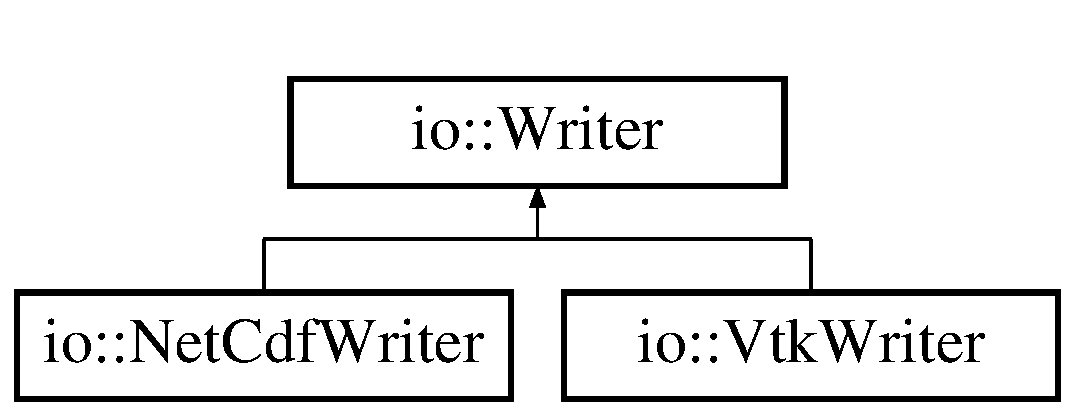
\includegraphics[height=2.000000cm]{classio_1_1Writer}
\end{center}
\end{figure}
\subsection*{Public Member Functions}
\begin{DoxyCompactItemize}
\item 
{\bf Writer} (const std\-::string \&i\-\_\-file\-Name, const {\bf Float2\-D} \&i\-\_\-b, const {\bf Boundary\-Size} \&i\-\_\-boundary\-Size, int i\-\_\-n\-X, int i\-\_\-n\-Y)
\item 
virtual void {\bf write\-Time\-Step} (const {\bf Float2\-D} \&i\-\_\-h, const {\bf Float2\-D} \&i\-\_\-hu, const {\bf Float2\-D} \&i\-\_\-hv, float i\-\_\-time)=0
\end{DoxyCompactItemize}
\subsection*{Protected Attributes}
\begin{DoxyCompactItemize}
\item 
const std\-::string {\bf file\-Name}\label{classio_1_1Writer_a93b978e8cbfc6bcf6dbfdc3f393d300a}

\begin{DoxyCompactList}\small\item\em file name of the data file \end{DoxyCompactList}\item 
const {\bf Float2\-D} \& {\bf b}\label{classio_1_1Writer_a1f5d4ab8728ae1c2ceba52c6c822d0bc}

\begin{DoxyCompactList}\small\item\em (Reference) to bathymetry data \end{DoxyCompactList}\item 
const {\bf Boundary\-Size} {\bf boundary\-Size}\label{classio_1_1Writer_a7cf701232192c20c41cbb4454601c219}

\begin{DoxyCompactList}\small\item\em Boundary layer size. \end{DoxyCompactList}\item 
const unsigned int {\bf n\-X}\label{classio_1_1Writer_a080fc86da3b2d8ea130382917d96252d}

\begin{DoxyCompactList}\small\item\em dimensions of the grid in x-\/ and y-\/direction. \end{DoxyCompactList}\item 
const unsigned int {\bfseries n\-Y}\label{classio_1_1Writer_a8c4ceaedd4b3e571cc4a5cacbcb21604}

\item 
size\-\_\-t {\bf time\-Step}\label{classio_1_1Writer_aa21f3ee8a54cf9278d711fe4f454f45c}

\begin{DoxyCompactList}\small\item\em current time step \end{DoxyCompactList}\end{DoxyCompactItemize}


\subsection{Constructor \& Destructor Documentation}
\index{io\-::\-Writer@{io\-::\-Writer}!Writer@{Writer}}
\index{Writer@{Writer}!io::Writer@{io\-::\-Writer}}
\subsubsection[{Writer}]{\setlength{\rightskip}{0pt plus 5cm}io\-::\-Writer\-::\-Writer (
\begin{DoxyParamCaption}
\item[{const std\-::string \&}]{i\-\_\-file\-Name, }
\item[{const {\bf Float2\-D} \&}]{i\-\_\-b, }
\item[{const {\bf Boundary\-Size} \&}]{i\-\_\-boundary\-Size, }
\item[{int}]{i\-\_\-n\-X, }
\item[{int}]{i\-\_\-n\-Y}
\end{DoxyParamCaption}
)\hspace{0.3cm}{\ttfamily [inline]}}\label{classio_1_1Writer_a6fe95f4a66e8b8ee1c9a52196ff3433f}

\begin{DoxyParams}{Parameters}
{\em i\-\_\-boundary\-Size} & size of the boundaries. \\
\hline
\end{DoxyParams}


\subsection{Member Function Documentation}
\index{io\-::\-Writer@{io\-::\-Writer}!write\-Time\-Step@{write\-Time\-Step}}
\index{write\-Time\-Step@{write\-Time\-Step}!io::Writer@{io\-::\-Writer}}
\subsubsection[{write\-Time\-Step}]{\setlength{\rightskip}{0pt plus 5cm}virtual void io\-::\-Writer\-::write\-Time\-Step (
\begin{DoxyParamCaption}
\item[{const {\bf Float2\-D} \&}]{i\-\_\-h, }
\item[{const {\bf Float2\-D} \&}]{i\-\_\-hu, }
\item[{const {\bf Float2\-D} \&}]{i\-\_\-hv, }
\item[{float}]{i\-\_\-time}
\end{DoxyParamCaption}
)\hspace{0.3cm}{\ttfamily [pure virtual]}}\label{classio_1_1Writer_a9ac05caa91aca4e79094d6718a2da16c}
Writes one time step


\begin{DoxyParams}{Parameters}
{\em i\-\_\-h} & water heights at a given time step. \\
\hline
{\em i\-\_\-hu} & momentums in x-\/direction at a given time step. \\
\hline
{\em i\-\_\-hv} & momentums in y-\/direction at a given time step. \\
\hline
{\em i\-\_\-time} & simulation time of the time step. \\
\hline
\end{DoxyParams}


Implemented in {\bf io\-::\-Net\-Cdf\-Writer} \doxyref{}{p.}{classio_1_1NetCdfWriter_a8e49f21f16b1720a348de50485754b0c}, and {\bf io\-::\-Vtk\-Writer} \doxyref{}{p.}{classio_1_1VtkWriter_ad464e594a34f4cd94b02087a2fade7bf}.



The documentation for this class was generated from the following file\-:\begin{DoxyCompactItemize}
\item 
src/writer/{\bf Writer.\-hh}\end{DoxyCompactItemize}

\chapter{File Documentation}
\section{src/blocks/cuda/\-S\-W\-E\-\_\-\-Block\-C\-U\-D\-A.hh File Reference}
\label{SWE__BlockCUDA_8hh}\index{src/blocks/cuda/\-S\-W\-E\-\_\-\-Block\-C\-U\-D\-A.\-hh@{src/blocks/cuda/\-S\-W\-E\-\_\-\-Block\-C\-U\-D\-A.\-hh}}
{\ttfamily \#include \char`\"{}blocks/\-S\-W\-E\-\_\-\-Block.\-hh\char`\"{}}\\*
{\ttfamily \#include \char`\"{}tools/help.\-hh\char`\"{}}\\*
{\ttfamily \#include $<$iostream$>$}\\*
{\ttfamily \#include $<$fstream$>$}\\*
{\ttfamily \#include $<$cuda\-\_\-runtime.\-h$>$}\\*
\subsection*{Classes}
\begin{DoxyCompactItemize}
\item 
class {\bf S\-W\-E\-\_\-\-Block\-C\-U\-D\-A}
\end{DoxyCompactItemize}
\subsection*{Functions}
\begin{DoxyCompactItemize}
\item 
void {\bfseries check\-C\-U\-D\-A\-Error} (const char $\ast$msg)\label{SWE__BlockCUDA_8hh_a3b360c7adecc62da0141b3c82e753c77}

\item 
void {\bfseries try\-C\-U\-D\-A} (cuda\-Error\-\_\-t err, const char $\ast$msg)\label{SWE__BlockCUDA_8hh_a0cda924127c6de7246554ed6b80917e5}

\item 
\-\_\-\-\_\-device\-\_\-\-\_\- int {\bf get\-Cell\-Coord} (int x, int y, int ny)
\item 
\-\_\-\-\_\-device\-\_\-\-\_\- int {\bf get\-Edge\-Coord} (int x, int y, int ny)
\item 
\-\_\-\-\_\-device\-\_\-\-\_\- int {\bf get\-Bathy\-Coord} (int x, int y, int ny)
\end{DoxyCompactItemize}
\subsection*{Variables}
\begin{DoxyCompactItemize}
\item 
const int {\bfseries T\-I\-L\-E\-\_\-\-S\-I\-Z\-E} =16\label{SWE__BlockCUDA_8hh_a8adcd57e318ecb77a2ffe6ec188f005b}

\end{DoxyCompactItemize}


\subsection{Detailed Description}
This file is part of S\-W\-E.

\begin{DoxyAuthor}{Author}
Michael Bader, Kaveh Rahnema, Tobias Schnabel 

Sebastian Rettenberger (rettenbs A\-T in.\-tum.\-de, {\tt http\-://www5.\-in.\-tum.\-de/wiki/index.\-php/\-Sebastian\-\_\-\-Rettenberger,\-\_\-\-M.\-Sc}.)
\end{DoxyAuthor}
\subsection{L\-I\-C\-E\-N\-S\-E}\label{Writer_8hh_LICENSE}
S\-W\-E is free software\-: you can redistribute it and/or modify it under the terms of the G\-N\-U General Public License as published by the Free Software Foundation, either version 3 of the License, or (at your option) any later version.

S\-W\-E is distributed in the hope that it will be useful, but W\-I\-T\-H\-O\-U\-T A\-N\-Y W\-A\-R\-R\-A\-N\-T\-Y; without even the implied warranty of M\-E\-R\-C\-H\-A\-N\-T\-A\-B\-I\-L\-I\-T\-Y or F\-I\-T\-N\-E\-S\-S F\-O\-R A P\-A\-R\-T\-I\-C\-U\-L\-A\-R P\-U\-R\-P\-O\-S\-E. See the G\-N\-U General Public License for more details.

You should have received a copy of the G\-N\-U General Public License along with S\-W\-E. If not, see {\tt http\-://www.\-gnu.\-org/licenses/}.\subsection{D\-E\-S\-C\-R\-I\-P\-T\-I\-O\-N}\label{NetCdfWriter_8hh_DESCRIPTION}
T\-O\-D\-O 

\subsection{Function Documentation}
\index{S\-W\-E\-\_\-\-Block\-C\-U\-D\-A.\-hh@{S\-W\-E\-\_\-\-Block\-C\-U\-D\-A.\-hh}!get\-Bathy\-Coord@{get\-Bathy\-Coord}}
\index{get\-Bathy\-Coord@{get\-Bathy\-Coord}!SWE_BlockCUDA.hh@{S\-W\-E\-\_\-\-Block\-C\-U\-D\-A.\-hh}}
\subsubsection[{get\-Bathy\-Coord}]{\setlength{\rightskip}{0pt plus 5cm}\-\_\-\-\_\-device\-\_\-\-\_\- int get\-Bathy\-Coord (
\begin{DoxyParamCaption}
\item[{int}]{x, }
\item[{int}]{y, }
\item[{int}]{ny}
\end{DoxyParamCaption}
)\hspace{0.3cm}{\ttfamily [inline]}}\label{SWE__BlockCUDA_8hh_add74cf6e6e3f322a5948a74fc7183cde}
Return index of a specific element in the arrays of bathymetry source terms 
\begin{DoxyParams}{Parameters}
{\em i,j} & x-\/ and y-\/coordinate of grid cell \\
\hline
{\em ny} & grid size in y-\/direction (without ghost layers) \\
\hline
\end{DoxyParams}
\index{S\-W\-E\-\_\-\-Block\-C\-U\-D\-A.\-hh@{S\-W\-E\-\_\-\-Block\-C\-U\-D\-A.\-hh}!get\-Cell\-Coord@{get\-Cell\-Coord}}
\index{get\-Cell\-Coord@{get\-Cell\-Coord}!SWE_BlockCUDA.hh@{S\-W\-E\-\_\-\-Block\-C\-U\-D\-A.\-hh}}
\subsubsection[{get\-Cell\-Coord}]{\setlength{\rightskip}{0pt plus 5cm}\-\_\-\-\_\-device\-\_\-\-\_\- int get\-Cell\-Coord (
\begin{DoxyParamCaption}
\item[{int}]{x, }
\item[{int}]{y, }
\item[{int}]{ny}
\end{DoxyParamCaption}
)\hspace{0.3cm}{\ttfamily [inline]}}\label{SWE__BlockCUDA_8hh_a851d73679072ec13f3e3a9bd9dd4ddcc}
Return index of hd[i][j] in linearised array 
\begin{DoxyParams}{Parameters}
{\em i,j} & x-\/ and y-\/coordinate of grid cell \\
\hline
{\em ny} & grid size in y-\/direction (without ghost layers) \\
\hline
\end{DoxyParams}
\index{S\-W\-E\-\_\-\-Block\-C\-U\-D\-A.\-hh@{S\-W\-E\-\_\-\-Block\-C\-U\-D\-A.\-hh}!get\-Edge\-Coord@{get\-Edge\-Coord}}
\index{get\-Edge\-Coord@{get\-Edge\-Coord}!SWE_BlockCUDA.hh@{S\-W\-E\-\_\-\-Block\-C\-U\-D\-A.\-hh}}
\subsubsection[{get\-Edge\-Coord}]{\setlength{\rightskip}{0pt plus 5cm}\-\_\-\-\_\-device\-\_\-\-\_\- int get\-Edge\-Coord (
\begin{DoxyParamCaption}
\item[{int}]{x, }
\item[{int}]{y, }
\item[{int}]{ny}
\end{DoxyParamCaption}
)\hspace{0.3cm}{\ttfamily [inline]}}\label{SWE__BlockCUDA_8hh_acbd2e57b95983dbef453451ff7ddf9bb}
Return index of edge-\/data Fhd[i][j] or Ghd[i][j] in linearised array 
\begin{DoxyParams}{Parameters}
{\em i,j} & x-\/ and y-\/coordinate of grid cell \\
\hline
{\em ny} & grid size in y-\/direction (without ghost layers) \\
\hline
\end{DoxyParams}

\section{src/blocks/cuda/\-S\-W\-E\-\_\-\-Block\-C\-U\-D\-A\-\_\-kernels.hh File Reference}
\label{SWE__BlockCUDA__kernels_8hh}\index{src/blocks/cuda/\-S\-W\-E\-\_\-\-Block\-C\-U\-D\-A\-\_\-kernels.\-hh@{src/blocks/cuda/\-S\-W\-E\-\_\-\-Block\-C\-U\-D\-A\-\_\-kernels.\-hh}}
\subsection*{Functions}
\begin{DoxyCompactItemize}
\item 
\-\_\-\-\_\-global\-\_\-\-\_\- void {\bfseries kernel\-Hd\-Buffer\-Edges} (float $\ast$hd, int nx, int ny)\label{SWE__BlockCUDA__kernels_8hh_ad34d42b9197cf6063931cb1bf7c03bd4}

\item 
\-\_\-\-\_\-global\-\_\-\-\_\- void {\bfseries kernel\-Maximum} (float $\ast$maxhd, float $\ast$maxvd, int start, int size)\label{SWE__BlockCUDA__kernels_8hh_ae810017f0a27a38e1c5d78c7130e8ab4}

\item 
\-\_\-\-\_\-global\-\_\-\-\_\- void {\bfseries kernel\-Left\-Boundary} (float $\ast$hd, float $\ast$hud, float $\ast$hvd, int nx, int ny, {\bf Boundary\-Type} bound)\label{SWE__BlockCUDA__kernels_8hh_a70e795bea06be7152de387957e090eb3}

\item 
\-\_\-\-\_\-global\-\_\-\-\_\- void {\bfseries kernel\-Right\-Boundary} (float $\ast$hd, float $\ast$hud, float $\ast$hvd, int nx, int ny, {\bf Boundary\-Type} bound)\label{SWE__BlockCUDA__kernels_8hh_a5b25e2843f0f18a4a5843165ce46054f}

\item 
\-\_\-\-\_\-global\-\_\-\-\_\- void {\bfseries kernel\-Bottom\-Boundary} (float $\ast$hd, float $\ast$hud, float $\ast$hvd, int nx, int ny, {\bf Boundary\-Type} bound)\label{SWE__BlockCUDA__kernels_8hh_a776336452fee130d27d02b109a7ab89d}

\item 
\-\_\-\-\_\-global\-\_\-\-\_\- void {\bfseries kernel\-Top\-Boundary} (float $\ast$hd, float $\ast$hud, float $\ast$hvd, int nx, int ny, {\bf Boundary\-Type} bound)\label{SWE__BlockCUDA__kernels_8hh_a655f11967ba2a7ed124b92a9f1400788}

\item 
\-\_\-\-\_\-global\-\_\-\-\_\- void {\bfseries kernel\-Bottom\-Ghost\-Boundary} (float $\ast$hd, float $\ast$hud, float $\ast$hvd, float $\ast$bottom\-Ghost\-Layer, int nx, int ny)\label{SWE__BlockCUDA__kernels_8hh_a899b7431f0cec06555bf3b0d8e848782}

\item 
\-\_\-\-\_\-global\-\_\-\-\_\- void {\bfseries kernel\-Top\-Ghost\-Boundary} (float $\ast$hd, float $\ast$hud, float $\ast$hvd, float $\ast$top\-Ghost\-Layer, int nx, int ny)\label{SWE__BlockCUDA__kernels_8hh_a7cf7164d51b1b16664556c25dd675a46}

\item 
\-\_\-\-\_\-global\-\_\-\-\_\- void {\bfseries kernel\-Bottom\-Copy\-Layer} (float $\ast$hd, float $\ast$hud, float $\ast$hvd, float $\ast$bottom\-Copy\-Layer, int nx, int ny)\label{SWE__BlockCUDA__kernels_8hh_af1a79800b1a5fca1daaeded30541769b}

\item 
\-\_\-\-\_\-global\-\_\-\-\_\- void {\bfseries kernel\-Top\-Copy\-Layer} (float $\ast$hd, float $\ast$hud, float $\ast$hvd, float $\ast$top\-Copy\-Layer, int nx, int ny)\label{SWE__BlockCUDA__kernels_8hh_a48b8d7d4d3bf3c69a289df057f4b6f3e}

\end{DoxyCompactItemize}


\subsection{Detailed Description}
This file is part of S\-W\-E.

\begin{DoxyAuthor}{Author}
Michael Bader (bader A\-T in.\-tum.\-de, {\tt http\-://www5.\-in.\-tum.\-de/wiki/index.\-php/\-Univ.-\/\-Prof.\-\_\-\-Dr.\-\_\-\-Michael\-\_\-\-Bader})
\end{DoxyAuthor}
\subsection{L\-I\-C\-E\-N\-S\-E}\label{Writer_8hh_LICENSE}
S\-W\-E is free software\-: you can redistribute it and/or modify it under the terms of the G\-N\-U General Public License as published by the Free Software Foundation, either version 3 of the License, or (at your option) any later version.

S\-W\-E is distributed in the hope that it will be useful, but W\-I\-T\-H\-O\-U\-T A\-N\-Y W\-A\-R\-R\-A\-N\-T\-Y; without even the implied warranty of M\-E\-R\-C\-H\-A\-N\-T\-A\-B\-I\-L\-I\-T\-Y or F\-I\-T\-N\-E\-S\-S F\-O\-R A P\-A\-R\-T\-I\-C\-U\-L\-A\-R P\-U\-R\-P\-O\-S\-E. See the G\-N\-U General Public License for more details.

You should have received a copy of the G\-N\-U General Public License along with S\-W\-E. If not, see {\tt http\-://www.\-gnu.\-org/licenses/}.\subsection{D\-E\-S\-C\-R\-I\-P\-T\-I\-O\-N}\label{NetCdfWriter_8hh_DESCRIPTION}
T\-O\-D\-O 
\section{src/blocks/cuda/\-S\-W\-E\-\_\-\-Wave\-Propagation\-Block\-Cuda.hh File Reference}
\label{SWE__WavePropagationBlockCuda_8hh}\index{src/blocks/cuda/\-S\-W\-E\-\_\-\-Wave\-Propagation\-Block\-Cuda.\-hh@{src/blocks/cuda/\-S\-W\-E\-\_\-\-Wave\-Propagation\-Block\-Cuda.\-hh}}
{\ttfamily \#include $<$cassert$>$}\\*
{\ttfamily \#include \char`\"{}S\-W\-E\-\_\-\-Block\-C\-U\-D\-A.\-hh\char`\"{}}\\*
\subsection*{Classes}
\begin{DoxyCompactItemize}
\item 
class {\bf S\-W\-E\-\_\-\-Wave\-Propagation\-Block\-Cuda}
\end{DoxyCompactItemize}


\subsection{Detailed Description}
This file is part of S\-W\-E.

\begin{DoxyAuthor}{Author}
Alexander Breuer (breuera A\-T in.\-tum.\-de, {\tt http\-://www5.\-in.\-tum.\-de/wiki/index.\-php/\-Dipl.-\/\-Math.\-\_\-\-Alexander\-\_\-\-Breuer}) 

Sebastian Rettenberger (rettenbs A\-T in.\-tum.\-de, {\tt http\-://www5.\-in.\-tum.\-de/wiki/index.\-php/\-Sebastian\-\_\-\-Rettenberger,\-\_\-\-M.\-Sc}.)
\end{DoxyAuthor}
\subsection{L\-I\-C\-E\-N\-S\-E}\label{Writer_8hh_LICENSE}
S\-W\-E is free software\-: you can redistribute it and/or modify it under the terms of the G\-N\-U General Public License as published by the Free Software Foundation, either version 3 of the License, or (at your option) any later version.

S\-W\-E is distributed in the hope that it will be useful, but W\-I\-T\-H\-O\-U\-T A\-N\-Y W\-A\-R\-R\-A\-N\-T\-Y; without even the implied warranty of M\-E\-R\-C\-H\-A\-N\-T\-A\-B\-I\-L\-I\-T\-Y or F\-I\-T\-N\-E\-S\-S F\-O\-R A P\-A\-R\-T\-I\-C\-U\-L\-A\-R P\-U\-R\-P\-O\-S\-E. See the G\-N\-U General Public License for more details.

You should have received a copy of the G\-N\-U General Public License along with S\-W\-E. If not, see {\tt http\-://www.\-gnu.\-org/licenses/}.\subsection{D\-E\-S\-C\-R\-I\-P\-T\-I\-O\-N}\label{NetCdfWriter_8hh_DESCRIPTION}
\doxyref{S\-W\-E\-\_\-\-Block}{p.}{classSWE__Block} in C\-U\-D\-A, which uses solvers in the wave propagation formulation. 
\section{src/blocks/cuda/\-S\-W\-E\-\_\-\-Wave\-Propagation\-Block\-Cuda\-\_\-kernels.hh File Reference}
\label{SWE__WavePropagationBlockCuda__kernels_8hh}\index{src/blocks/cuda/\-S\-W\-E\-\_\-\-Wave\-Propagation\-Block\-Cuda\-\_\-kernels.\-hh@{src/blocks/cuda/\-S\-W\-E\-\_\-\-Wave\-Propagation\-Block\-Cuda\-\_\-kernels.\-hh}}
\subsection*{Functions}
\begin{DoxyCompactItemize}
\item 
\-\_\-\-\_\-global\-\_\-\-\_\- void {\bfseries compute\-Net\-Updates\-Kernel} (const float $\ast$i\-\_\-h, const float $\ast$i\-\_\-hu, const float $\ast$i\-\_\-hv, const float $\ast$i\-\_\-b, float $\ast$o\-\_\-h\-Net\-Updates\-Left\-D, float $\ast$o\-\_\-h\-Net\-Updates\-Right\-D, float $\ast$o\-\_\-hu\-Net\-Updates\-Left\-D, float $\ast$o\-\_\-hu\-Net\-Updates\-Right\-D, float $\ast$o\-\_\-h\-Net\-Updates\-Below\-D, float $\ast$o\-\_\-h\-Net\-Updates\-Above\-D, float $\ast$o\-\_\-hv\-Net\-Updates\-Below\-D, float $\ast$o\-\_\-hv\-Net\-Updates\-Above\-D, float $\ast$o\-\_\-maximum\-Wave\-Speeds, const int i\-\_\-nx, const int i\-\_\-ny, const int i\-\_\-offset\-X=0, const int i\-\_\-offset\-Y=0, const int i\-\_\-block\-Off\-Set\-X=0, const int i\-\_\-block\-Off\-Set\-Y=0)\label{SWE__WavePropagationBlockCuda__kernels_8hh_a2bc584d7ead34df704e1c977c38c98bf}

\item 
\-\_\-\-\_\-global\-\_\-\-\_\- void {\bfseries update\-Unknowns\-Kernel} (const float $\ast$i\-\_\-h\-Net\-Updates\-Left\-D, const float $\ast$i\-\_\-h\-Net\-Updates\-Right\-D, const float $\ast$i\-\_\-hu\-Net\-Updates\-Left\-D, const float $\ast$i\-\_\-hu\-Net\-Updates\-Right\-D, const float $\ast$i\-\_\-h\-Net\-Updates\-Below\-D, const float $\ast$i\-\_\-h\-Net\-Updates\-Above\-D, const float $\ast$i\-\_\-hv\-Net\-Updates\-Below\-D, const float $\ast$i\-\_\-hv\-Net\-Updates\-Above\-D, float $\ast$io\-\_\-h, float $\ast$io\-\_\-hu, float $\ast$io\-\_\-hv, const float i\-\_\-update\-Width\-X, const float i\-\_\-update\-Width\-Y, const int i\-\_\-nx, const int i\-\_\-ny)\label{SWE__WavePropagationBlockCuda__kernels_8hh_a8b864dfc09bf8e43d7f2849fb74add2e}

\item 
\-\_\-\-\_\-device\-\_\-\-\_\- int {\bfseries compute\-One\-D\-Position\-Kernel} (const int i\-\_\-i, const int i\-\_\-j, const int i\-\_\-nx)\label{SWE__WavePropagationBlockCuda__kernels_8hh_aa1828414f270d255b05e877dd2f8b7df}

\end{DoxyCompactItemize}


\subsection{Detailed Description}
This file is part of S\-W\-E.

\begin{DoxyAuthor}{Author}
Alexander Breuer (breuera A\-T in.\-tum.\-de, {\tt http\-://www5.\-in.\-tum.\-de/wiki/index.\-php/\-Dipl.-\/\-Math.\-\_\-\-Alexander\-\_\-\-Breuer})
\end{DoxyAuthor}
\subsection{L\-I\-C\-E\-N\-S\-E}\label{Writer_8hh_LICENSE}
S\-W\-E is free software\-: you can redistribute it and/or modify it under the terms of the G\-N\-U General Public License as published by the Free Software Foundation, either version 3 of the License, or (at your option) any later version.

S\-W\-E is distributed in the hope that it will be useful, but W\-I\-T\-H\-O\-U\-T A\-N\-Y W\-A\-R\-R\-A\-N\-T\-Y; without even the implied warranty of M\-E\-R\-C\-H\-A\-N\-T\-A\-B\-I\-L\-I\-T\-Y or F\-I\-T\-N\-E\-S\-S F\-O\-R A P\-A\-R\-T\-I\-C\-U\-L\-A\-R P\-U\-R\-P\-O\-S\-E. See the G\-N\-U General Public License for more details.

You should have received a copy of the G\-N\-U General Public License along with S\-W\-E. If not, see {\tt http\-://www.\-gnu.\-org/licenses/}.\subsection{D\-E\-S\-C\-R\-I\-P\-T\-I\-O\-N}\label{NetCdfWriter_8hh_DESCRIPTION}
C\-U\-D\-A Kernels for a \doxyref{S\-W\-E\-\_\-\-Block}{p.}{classSWE__Block}, which uses solvers in the wave propagation formulation. 
\section{src/blocks/rusanov/\-S\-W\-E\-\_\-\-Rusanov\-Block.cpp File Reference}
\label{SWE__RusanovBlock_8cpp}\index{src/blocks/rusanov/\-S\-W\-E\-\_\-\-Rusanov\-Block.\-cpp@{src/blocks/rusanov/\-S\-W\-E\-\_\-\-Rusanov\-Block.\-cpp}}
{\ttfamily \#include \char`\"{}S\-W\-E\-\_\-\-Rusanov\-Block.\-hh\char`\"{}}\\*
{\ttfamily \#include $<$math.\-h$>$}\\*
\subsection*{Functions}
\begin{DoxyCompactItemize}
\item 
ostream \& {\bf operator$<$$<$} (ostream \&os, const {\bf S\-W\-E\-\_\-\-Rusanov\-Block} \&swe)
\end{DoxyCompactItemize}


\subsection{Detailed Description}
This file is part of S\-W\-E.

\begin{DoxyAuthor}{Author}
Michael Bader, Kaveh Rahnema, Tobias Schnabel
\end{DoxyAuthor}
\subsection{L\-I\-C\-E\-N\-S\-E}\label{Writer_8hh_LICENSE}
S\-W\-E is free software\-: you can redistribute it and/or modify it under the terms of the G\-N\-U General Public License as published by the Free Software Foundation, either version 3 of the License, or (at your option) any later version.

S\-W\-E is distributed in the hope that it will be useful, but W\-I\-T\-H\-O\-U\-T A\-N\-Y W\-A\-R\-R\-A\-N\-T\-Y; without even the implied warranty of M\-E\-R\-C\-H\-A\-N\-T\-A\-B\-I\-L\-I\-T\-Y or F\-I\-T\-N\-E\-S\-S F\-O\-R A P\-A\-R\-T\-I\-C\-U\-L\-A\-R P\-U\-R\-P\-O\-S\-E. See the G\-N\-U General Public License for more details.

You should have received a copy of the G\-N\-U General Public License along with S\-W\-E. If not, see {\tt http\-://www.\-gnu.\-org/licenses/}.\subsection{D\-E\-S\-C\-R\-I\-P\-T\-I\-O\-N}\label{NetCdfWriter_8hh_DESCRIPTION}
T\-O\-D\-O 

\subsection{Function Documentation}
\index{S\-W\-E\-\_\-\-Rusanov\-Block.\-cpp@{S\-W\-E\-\_\-\-Rusanov\-Block.\-cpp}!operator$<$$<$@{operator$<$$<$}}
\index{operator$<$$<$@{operator$<$$<$}!SWE_RusanovBlock.cpp@{S\-W\-E\-\_\-\-Rusanov\-Block.\-cpp}}
\subsubsection[{operator$<$$<$}]{\setlength{\rightskip}{0pt plus 5cm}ostream\& operator$<$$<$ (
\begin{DoxyParamCaption}
\item[{ostream \&}]{os, }
\item[{const {\bf S\-W\-E\-\_\-\-Rusanov\-Block} \&}]{swe}
\end{DoxyParamCaption}
)}\label{SWE__RusanovBlock_8cpp_a11f96afabd5e590e50d491568b96503a}
overload operator$<$$<$ such that data can be written via cout $<$$<$ -\/$>$ needs to be declared as friend to be allowed to access private data 
\section{src/blocks/rusanov/\-S\-W\-E\-\_\-\-Rusanov\-Block.hh File Reference}
\label{SWE__RusanovBlock_8hh}\index{src/blocks/rusanov/\-S\-W\-E\-\_\-\-Rusanov\-Block.\-hh@{src/blocks/rusanov/\-S\-W\-E\-\_\-\-Rusanov\-Block.\-hh}}
{\ttfamily \#include $<$iostream$>$}\\*
{\ttfamily \#include $<$stdio.\-h$>$}\\*
{\ttfamily \#include $<$fstream$>$}\\*
{\ttfamily \#include \char`\"{}tools/help.\-hh\char`\"{}}\\*
{\ttfamily \#include \char`\"{}S\-W\-E\-\_\-\-Block.\-hh\char`\"{}}\\*
\subsection*{Classes}
\begin{DoxyCompactItemize}
\item 
class {\bf S\-W\-E\-\_\-\-Rusanov\-Block}
\end{DoxyCompactItemize}
\subsection*{Functions}
\begin{DoxyCompactItemize}
\item 
ostream \& {\bf operator$<$$<$} (ostream \&os, const {\bf S\-W\-E\-\_\-\-Rusanov\-Block} \&swe)
\end{DoxyCompactItemize}


\subsection{Detailed Description}
This file is part of S\-W\-E.

\begin{DoxyAuthor}{Author}
Michael Bader, Kaveh Rahnema, Tobias Schnabel
\end{DoxyAuthor}
\subsection{L\-I\-C\-E\-N\-S\-E}\label{Writer_8hh_LICENSE}
S\-W\-E is free software\-: you can redistribute it and/or modify it under the terms of the G\-N\-U General Public License as published by the Free Software Foundation, either version 3 of the License, or (at your option) any later version.

S\-W\-E is distributed in the hope that it will be useful, but W\-I\-T\-H\-O\-U\-T A\-N\-Y W\-A\-R\-R\-A\-N\-T\-Y; without even the implied warranty of M\-E\-R\-C\-H\-A\-N\-T\-A\-B\-I\-L\-I\-T\-Y or F\-I\-T\-N\-E\-S\-S F\-O\-R A P\-A\-R\-T\-I\-C\-U\-L\-A\-R P\-U\-R\-P\-O\-S\-E. See the G\-N\-U General Public License for more details.

You should have received a copy of the G\-N\-U General Public License along with S\-W\-E. If not, see {\tt http\-://www.\-gnu.\-org/licenses/}.\subsection{D\-E\-S\-C\-R\-I\-P\-T\-I\-O\-N}\label{NetCdfWriter_8hh_DESCRIPTION}
T\-O\-D\-O 

\subsection{Function Documentation}
\index{S\-W\-E\-\_\-\-Rusanov\-Block.\-hh@{S\-W\-E\-\_\-\-Rusanov\-Block.\-hh}!operator$<$$<$@{operator$<$$<$}}
\index{operator$<$$<$@{operator$<$$<$}!SWE_RusanovBlock.hh@{S\-W\-E\-\_\-\-Rusanov\-Block.\-hh}}
\subsubsection[{operator$<$$<$}]{\setlength{\rightskip}{0pt plus 5cm}ostream\& operator$<$$<$ (
\begin{DoxyParamCaption}
\item[{ostream \&}]{os, }
\item[{const {\bf S\-W\-E\-\_\-\-Rusanov\-Block} \&}]{swe}
\end{DoxyParamCaption}
)}\label{SWE__RusanovBlock_8hh_a11f96afabd5e590e50d491568b96503a}
overload operator$<$$<$ such that data can be written via cout $<$$<$ -\/$>$ needs to be declared as friend to be allowed to access private data 
\section{src/blocks/rusanov/\-S\-W\-E\-\_\-\-Rusanov\-Block\-C\-U\-D\-A.hh File Reference}
\label{SWE__RusanovBlockCUDA_8hh}\index{src/blocks/rusanov/\-S\-W\-E\-\_\-\-Rusanov\-Block\-C\-U\-D\-A.\-hh@{src/blocks/rusanov/\-S\-W\-E\-\_\-\-Rusanov\-Block\-C\-U\-D\-A.\-hh}}
{\ttfamily \#include $<$iostream$>$}\\*
{\ttfamily \#include $<$stdio.\-h$>$}\\*
{\ttfamily \#include $<$fstream$>$}\\*
{\ttfamily \#include $<$cuda\-\_\-runtime.\-h$>$}\\*
{\ttfamily \#include \char`\"{}tools/help.\-hh\char`\"{}}\\*
{\ttfamily \#include \char`\"{}S\-W\-E\-\_\-\-Block.\-hh\char`\"{}}\\*
{\ttfamily \#include \char`\"{}S\-W\-E\-\_\-\-Block\-C\-U\-D\-A.\-hh\char`\"{}}\\*
\subsection*{Classes}
\begin{DoxyCompactItemize}
\item 
class {\bf S\-W\-E\-\_\-\-Rusanov\-Block\-C\-U\-D\-A}
\end{DoxyCompactItemize}
\subsection*{Functions}
\begin{DoxyCompactItemize}
\item 
ostream \& {\bfseries operator$<$$<$} (ostream \&os, const {\bf S\-W\-E\-\_\-\-Rusanov\-Block\-C\-U\-D\-A} \&swe)\label{SWE__RusanovBlockCUDA_8hh_adbdcb6417643b695657724ea16f84954}

\end{DoxyCompactItemize}


\subsection{Detailed Description}
This file is part of S\-W\-E.

\begin{DoxyAuthor}{Author}
Michael Bader, Kaveh Rahnema, Tobias Schnabel
\end{DoxyAuthor}
\subsection{L\-I\-C\-E\-N\-S\-E}\label{Writer_8hh_LICENSE}
S\-W\-E is free software\-: you can redistribute it and/or modify it under the terms of the G\-N\-U General Public License as published by the Free Software Foundation, either version 3 of the License, or (at your option) any later version.

S\-W\-E is distributed in the hope that it will be useful, but W\-I\-T\-H\-O\-U\-T A\-N\-Y W\-A\-R\-R\-A\-N\-T\-Y; without even the implied warranty of M\-E\-R\-C\-H\-A\-N\-T\-A\-B\-I\-L\-I\-T\-Y or F\-I\-T\-N\-E\-S\-S F\-O\-R A P\-A\-R\-T\-I\-C\-U\-L\-A\-R P\-U\-R\-P\-O\-S\-E. See the G\-N\-U General Public License for more details.

You should have received a copy of the G\-N\-U General Public License along with S\-W\-E. If not, see {\tt http\-://www.\-gnu.\-org/licenses/}.\subsection{D\-E\-S\-C\-R\-I\-P\-T\-I\-O\-N}\label{NetCdfWriter_8hh_DESCRIPTION}
T\-O\-D\-O 
\section{src/blocks/rusanov/\-S\-W\-E\-\_\-\-Rusanov\-Block\-C\-U\-D\-A\-\_\-kernels.hh File Reference}
\label{SWE__RusanovBlockCUDA__kernels_8hh}\index{src/blocks/rusanov/\-S\-W\-E\-\_\-\-Rusanov\-Block\-C\-U\-D\-A\-\_\-kernels.\-hh@{src/blocks/rusanov/\-S\-W\-E\-\_\-\-Rusanov\-Block\-C\-U\-D\-A\-\_\-kernels.\-hh}}
\subsection*{Functions}
\begin{DoxyCompactItemize}
\item 
\-\_\-\-\_\-global\-\_\-\-\_\- void {\bfseries kernel\-Compute\-Fluxes\-F} (float $\ast$hd, float $\ast$hud, float $\ast$hvd, float $\ast$Fhd, float $\ast$Fhud, float $\ast$Fhvd, int ny, float g, float llf, int istart)\label{SWE__RusanovBlockCUDA__kernels_8hh_a125f373796424316bc49a0eb60f5f90e}

\item 
\-\_\-\-\_\-global\-\_\-\-\_\- void {\bfseries kernel\-Compute\-Fluxes\-G} (float $\ast$hd, float $\ast$hud, float $\ast$hvd, float $\ast$Ghd, float $\ast$Ghud, float $\ast$Ghvd, int ny, float g, float llf, int jstart)\label{SWE__RusanovBlockCUDA__kernels_8hh_a4a5d67e82c837347e337904d4c17cc07}

\item 
\-\_\-\-\_\-global\-\_\-\-\_\- void {\bfseries kernel\-Compute\-Bathymetry\-Sources} (float $\ast$hd, float $\ast$bd, float $\ast$Bxd, float $\ast$Byd, int ny, float g)\label{SWE__RusanovBlockCUDA__kernels_8hh_aa7530530448af30119436099351cfead}

\item 
\-\_\-\-\_\-global\-\_\-\-\_\- void {\bfseries kernel\-Euler\-Timestep} (float $\ast$hd, float $\ast$hud, float $\ast$hvd, float $\ast$Fhd, float $\ast$Fhud, float $\ast$Fhvd, float $\ast$Ghd, float $\ast$Ghud, float $\ast$Ghvd, float $\ast$Bxd, float $\ast$Byd, float $\ast$maxhd, float $\ast$maxvd, int nx, int ny, float dt, float dxi, float dyi)\label{SWE__RusanovBlockCUDA__kernels_8hh_a105ff13519fe40ec2acbc182d5584a07}

\item 
\-\_\-\-\_\-global\-\_\-\-\_\- void {\bfseries kernel\-Maximum} (float $\ast$maxhd, float $\ast$maxvd, int start, int size)\label{SWE__RusanovBlockCUDA__kernels_8hh_ae810017f0a27a38e1c5d78c7130e8ab4}

\end{DoxyCompactItemize}


\subsection{Detailed Description}
This file is part of S\-W\-E.

\begin{DoxyAuthor}{Author}
Michael Bader, Kaveh Rahnema, Tobias Schnabel
\end{DoxyAuthor}
\subsection{L\-I\-C\-E\-N\-S\-E}\label{Writer_8hh_LICENSE}
S\-W\-E is free software\-: you can redistribute it and/or modify it under the terms of the G\-N\-U General Public License as published by the Free Software Foundation, either version 3 of the License, or (at your option) any later version.

S\-W\-E is distributed in the hope that it will be useful, but W\-I\-T\-H\-O\-U\-T A\-N\-Y W\-A\-R\-R\-A\-N\-T\-Y; without even the implied warranty of M\-E\-R\-C\-H\-A\-N\-T\-A\-B\-I\-L\-I\-T\-Y or F\-I\-T\-N\-E\-S\-S F\-O\-R A P\-A\-R\-T\-I\-C\-U\-L\-A\-R P\-U\-R\-P\-O\-S\-E. See the G\-N\-U General Public License for more details.

You should have received a copy of the G\-N\-U General Public License along with S\-W\-E. If not, see {\tt http\-://www.\-gnu.\-org/licenses/}.\subsection{D\-E\-S\-C\-R\-I\-P\-T\-I\-O\-N}\label{NetCdfWriter_8hh_DESCRIPTION}
T\-O\-D\-O 
\section{src/blocks/\-S\-W\-E\-\_\-\-Block.cpp File Reference}
\label{SWE__Block_8cpp}\index{src/blocks/\-S\-W\-E\-\_\-\-Block.\-cpp@{src/blocks/\-S\-W\-E\-\_\-\-Block.\-cpp}}
{\ttfamily \#include \char`\"{}S\-W\-E\-\_\-\-Block.\-hh\char`\"{}}\\*
{\ttfamily \#include \char`\"{}tools/help.\-hh\char`\"{}}\\*
{\ttfamily \#include \char`\"{}solvers/fsolver.\-cpp\char`\"{}}\\*
{\ttfamily \#include $<$cmath$>$}\\*
{\ttfamily \#include $<$iostream$>$}\\*
{\ttfamily \#include $<$cassert$>$}\\*
{\ttfamily \#include $<$limits$>$}\\*


\subsection{Detailed Description}
This file is part of S\-W\-E.

\begin{DoxyAuthor}{Author}
Michael Bader, Kaveh Rahnema, Tobias Schnabel 

Sebastian Rettenberger (rettenbs A\-T in.\-tum.\-de, {\tt http\-://www5.\-in.\-tum.\-de/wiki/index.\-php/\-Sebastian\-\_\-\-Rettenberger,\-\_\-\-M.\-Sc}.)
\end{DoxyAuthor}
\subsection{L\-I\-C\-E\-N\-S\-E}\label{Writer_8hh_LICENSE}
S\-W\-E is free software\-: you can redistribute it and/or modify it under the terms of the G\-N\-U General Public License as published by the Free Software Foundation, either version 3 of the License, or (at your option) any later version.

S\-W\-E is distributed in the hope that it will be useful, but W\-I\-T\-H\-O\-U\-T A\-N\-Y W\-A\-R\-R\-A\-N\-T\-Y; without even the implied warranty of M\-E\-R\-C\-H\-A\-N\-T\-A\-B\-I\-L\-I\-T\-Y or F\-I\-T\-N\-E\-S\-S F\-O\-R A P\-A\-R\-T\-I\-C\-U\-L\-A\-R P\-U\-R\-P\-O\-S\-E. See the G\-N\-U General Public License for more details.

You should have received a copy of the G\-N\-U General Public License along with S\-W\-E. If not, see {\tt http\-://www.\-gnu.\-org/licenses/}.\subsection{D\-E\-S\-C\-R\-I\-P\-T\-I\-O\-N}\label{NetCdfWriter_8hh_DESCRIPTION}
T\-O\-D\-O 
\section{src/blocks/\-S\-W\-E\-\_\-\-Block.hh File Reference}
\label{SWE__Block_8hh}\index{src/blocks/\-S\-W\-E\-\_\-\-Block.\-hh@{src/blocks/\-S\-W\-E\-\_\-\-Block.\-hh}}
{\ttfamily \#include \char`\"{}tools/help.\-hh\char`\"{}}\\*
{\ttfamily \#include \char`\"{}scenarios/\-S\-W\-E\-\_\-\-Scenario.\-hh\char`\"{}}\\*
{\ttfamily \#include $<$iostream$>$}\\*
{\ttfamily \#include $<$fstream$>$}\\*
\subsection*{Classes}
\begin{DoxyCompactItemize}
\item 
class {\bf S\-W\-E\-\_\-\-Block}
\item 
struct {\bf S\-W\-E\-\_\-\-Block1\-D}
\item 
class {\bf S\-W\-E\-\_\-\-Dimensional\-Splitting}
\end{DoxyCompactItemize}


\subsection{Detailed Description}
This file is part of S\-W\-E.

\begin{DoxyAuthor}{Author}
Michael Bader, Kaveh Rahnema, Tobias Schnabel 

Sebastian Rettenberger (rettenbs A\-T in.\-tum.\-de, {\tt http\-://www5.\-in.\-tum.\-de/wiki/index.\-php/\-Sebastian\-\_\-\-Rettenberger,\-\_\-\-M.\-Sc}.)
\end{DoxyAuthor}
\subsection{L\-I\-C\-E\-N\-S\-E}\label{Writer_8hh_LICENSE}
S\-W\-E is free software\-: you can redistribute it and/or modify it under the terms of the G\-N\-U General Public License as published by the Free Software Foundation, either version 3 of the License, or (at your option) any later version.

S\-W\-E is distributed in the hope that it will be useful, but W\-I\-T\-H\-O\-U\-T A\-N\-Y W\-A\-R\-R\-A\-N\-T\-Y; without even the implied warranty of M\-E\-R\-C\-H\-A\-N\-T\-A\-B\-I\-L\-I\-T\-Y or F\-I\-T\-N\-E\-S\-S F\-O\-R A P\-A\-R\-T\-I\-C\-U\-L\-A\-R P\-U\-R\-P\-O\-S\-E. See the G\-N\-U General Public License for more details.

You should have received a copy of the G\-N\-U General Public License along with S\-W\-E. If not, see {\tt http\-://www.\-gnu.\-org/licenses/}.\subsection{D\-E\-S\-C\-R\-I\-P\-T\-I\-O\-N}\label{NetCdfWriter_8hh_DESCRIPTION}
T\-O\-D\-O 
\section{src/blocks/\-S\-W\-E\-\_\-\-Wave\-Accumulation\-Block.cpp File Reference}
\label{SWE__WaveAccumulationBlock_8cpp}\index{src/blocks/\-S\-W\-E\-\_\-\-Wave\-Accumulation\-Block.\-cpp@{src/blocks/\-S\-W\-E\-\_\-\-Wave\-Accumulation\-Block.\-cpp}}
{\ttfamily \#include \char`\"{}S\-W\-E\-\_\-\-Wave\-Accumulation\-Block.\-hh\char`\"{}}\\*
{\ttfamily \#include $<$cassert$>$}\\*
{\ttfamily \#include $<$string$>$}\\*
{\ttfamily \#include $<$limits$>$}\\*


\subsection{Detailed Description}
This file is part of S\-W\-E.

\begin{DoxyAuthor}{Author}
Alexander Breuer (breuera A\-T in.\-tum.\-de, {\tt http\-://www5.\-in.\-tum.\-de/wiki/index.\-php/\-Dipl.-\/\-Math.\-\_\-\-Alexander\-\_\-\-Breuer}) 

Sebastian Rettenberger (rettenbs A\-T in.\-tum.\-de, {\tt http\-://www5.\-in.\-tum.\-de/wiki/index.\-php/\-Sebastian\-\_\-\-Rettenberger,\-\_\-\-M.\-Sc}.) 

Michael Bader (bader A\-T in.\-tum.\-de, {\tt http\-://www5.\-in.\-tum.\-de/wiki/index.\-php/\-Michael\-\_\-\-Bader})
\end{DoxyAuthor}
\subsection{L\-I\-C\-E\-N\-S\-E}\label{Writer_8hh_LICENSE}
S\-W\-E is free software\-: you can redistribute it and/or modify it under the terms of the G\-N\-U General Public License as published by the Free Software Foundation, either version 3 of the License, or (at your option) any later version.

S\-W\-E is distributed in the hope that it will be useful, but W\-I\-T\-H\-O\-U\-T A\-N\-Y W\-A\-R\-R\-A\-N\-T\-Y; without even the implied warranty of M\-E\-R\-C\-H\-A\-N\-T\-A\-B\-I\-L\-I\-T\-Y or F\-I\-T\-N\-E\-S\-S F\-O\-R A P\-A\-R\-T\-I\-C\-U\-L\-A\-R P\-U\-R\-P\-O\-S\-E. See the G\-N\-U General Public License for more details.

You should have received a copy of the G\-N\-U General Public License along with S\-W\-E. If not, see {\tt http\-://www.\-gnu.\-org/licenses/}.\subsection{D\-E\-S\-C\-R\-I\-P\-T\-I\-O\-N}\label{NetCdfWriter_8hh_DESCRIPTION}
\doxyref{S\-W\-E\-\_\-\-Block}{p.}{classSWE__Block}, which uses solvers in the wave propagation formulation. 
\section{src/blocks/\-S\-W\-E\-\_\-\-Wave\-Accumulation\-Block.hh File Reference}
\label{SWE__WaveAccumulationBlock_8hh}\index{src/blocks/\-S\-W\-E\-\_\-\-Wave\-Accumulation\-Block.\-hh@{src/blocks/\-S\-W\-E\-\_\-\-Wave\-Accumulation\-Block.\-hh}}
{\ttfamily \#include \char`\"{}blocks/\-S\-W\-E\-\_\-\-Block.\-hh\char`\"{}}\\*
{\ttfamily \#include \char`\"{}tools/help.\-hh\char`\"{}}\\*
{\ttfamily \#include $<$string$>$}\\*
\subsection*{Classes}
\begin{DoxyCompactItemize}
\item 
class {\bf S\-W\-E\-\_\-\-Wave\-Accumulation\-Block}
\end{DoxyCompactItemize}


\subsection{Detailed Description}
This file is part of S\-W\-E.

\begin{DoxyAuthor}{Author}
Alexander Breuer (breuera A\-T in.\-tum.\-de, {\tt http\-://www5.\-in.\-tum.\-de/wiki/index.\-php/\-Dipl.-\/\-Math.\-\_\-\-Alexander\-\_\-\-Breuer}) 

Sebastian Rettenberger (rettenbs A\-T in.\-tum.\-de, {\tt http\-://www5.\-in.\-tum.\-de/wiki/index.\-php/\-Sebastian\-\_\-\-Rettenberger,\-\_\-\-M.\-Sc}.) 

Michael Bader (bader A\-T in.\-tum.\-de, {\tt http\-://www5.\-in.\-tum.\-de/wiki/index.\-php/\-Michael\-\_\-\-Bader})
\end{DoxyAuthor}
\subsection{L\-I\-C\-E\-N\-S\-E}\label{Writer_8hh_LICENSE}
S\-W\-E is free software\-: you can redistribute it and/or modify it under the terms of the G\-N\-U General Public License as published by the Free Software Foundation, either version 3 of the License, or (at your option) any later version.

S\-W\-E is distributed in the hope that it will be useful, but W\-I\-T\-H\-O\-U\-T A\-N\-Y W\-A\-R\-R\-A\-N\-T\-Y; without even the implied warranty of M\-E\-R\-C\-H\-A\-N\-T\-A\-B\-I\-L\-I\-T\-Y or F\-I\-T\-N\-E\-S\-S F\-O\-R A P\-A\-R\-T\-I\-C\-U\-L\-A\-R P\-U\-R\-P\-O\-S\-E. See the G\-N\-U General Public License for more details.

You should have received a copy of the G\-N\-U General Public License along with S\-W\-E. If not, see {\tt http\-://www.\-gnu.\-org/licenses/}.\subsection{D\-E\-S\-C\-R\-I\-P\-T\-I\-O\-N}\label{NetCdfWriter_8hh_DESCRIPTION}
\doxyref{S\-W\-E\-\_\-\-Block}{p.}{classSWE__Block}, which uses solvers in the wave propagation formulation. 
\section{src/blocks/\-S\-W\-E\-\_\-\-Wave\-Propagation\-Block.cpp File Reference}
\label{SWE__WavePropagationBlock_8cpp}\index{src/blocks/\-S\-W\-E\-\_\-\-Wave\-Propagation\-Block.\-cpp@{src/blocks/\-S\-W\-E\-\_\-\-Wave\-Propagation\-Block.\-cpp}}
{\ttfamily \#include \char`\"{}S\-W\-E\-\_\-\-Wave\-Propagation\-Block.\-hh\char`\"{}}\\*
{\ttfamily \#include $<$cassert$>$}\\*
{\ttfamily \#include $<$string$>$}\\*
{\ttfamily \#include $<$limits$>$}\\*


\subsection{Detailed Description}
This file is part of S\-W\-E.

\begin{DoxyAuthor}{Author}
Alexander Breuer (breuera A\-T in.\-tum.\-de, {\tt http\-://www5.\-in.\-tum.\-de/wiki/index.\-php/\-Dipl.-\/\-Math.\-\_\-\-Alexander\-\_\-\-Breuer}) 

Sebastian Rettenberger (rettenbs A\-T in.\-tum.\-de, {\tt http\-://www5.\-in.\-tum.\-de/wiki/index.\-php/\-Sebastian\-\_\-\-Rettenberger,\-\_\-\-M.\-Sc}.) 

Michael Bader (bader A\-T in.\-tum.\-de, {\tt http\-://www5.\-in.\-tum.\-de/wiki/index.\-php/\-Michael\-\_\-\-Bader})
\end{DoxyAuthor}
\subsection{L\-I\-C\-E\-N\-S\-E}\label{Writer_8hh_LICENSE}
S\-W\-E is free software\-: you can redistribute it and/or modify it under the terms of the G\-N\-U General Public License as published by the Free Software Foundation, either version 3 of the License, or (at your option) any later version.

S\-W\-E is distributed in the hope that it will be useful, but W\-I\-T\-H\-O\-U\-T A\-N\-Y W\-A\-R\-R\-A\-N\-T\-Y; without even the implied warranty of M\-E\-R\-C\-H\-A\-N\-T\-A\-B\-I\-L\-I\-T\-Y or F\-I\-T\-N\-E\-S\-S F\-O\-R A P\-A\-R\-T\-I\-C\-U\-L\-A\-R P\-U\-R\-P\-O\-S\-E. See the G\-N\-U General Public License for more details.

You should have received a copy of the G\-N\-U General Public License along with S\-W\-E. If not, see {\tt http\-://www.\-gnu.\-org/licenses/}.\subsection{D\-E\-S\-C\-R\-I\-P\-T\-I\-O\-N}\label{NetCdfWriter_8hh_DESCRIPTION}
Implementation of \doxyref{S\-W\-E\-\_\-\-Block}{p.}{classSWE__Block} that uses solvers in the wave propagation formulation. 
\section{src/blocks/\-S\-W\-E\-\_\-\-Wave\-Propagation\-Block.hh File Reference}
\label{SWE__WavePropagationBlock_8hh}\index{src/blocks/\-S\-W\-E\-\_\-\-Wave\-Propagation\-Block.\-hh@{src/blocks/\-S\-W\-E\-\_\-\-Wave\-Propagation\-Block.\-hh}}
{\ttfamily \#include \char`\"{}blocks/\-S\-W\-E\-\_\-\-Block.\-hh\char`\"{}}\\*
{\ttfamily \#include \char`\"{}tools/help.\-hh\char`\"{}}\\*
{\ttfamily \#include $<$string$>$}\\*
{\ttfamily \#include \char`\"{}solvers/\-Hybrid.\-hpp\char`\"{}}\\*
\subsection*{Classes}
\begin{DoxyCompactItemize}
\item 
class {\bf S\-W\-E\-\_\-\-Wave\-Propagation\-Block}
\end{DoxyCompactItemize}


\subsection{Detailed Description}
This file is part of S\-W\-E.

\begin{DoxyAuthor}{Author}
Alexander Breuer (breuera A\-T in.\-tum.\-de, {\tt http\-://www5.\-in.\-tum.\-de/wiki/index.\-php/\-Dipl.-\/\-Math.\-\_\-\-Alexander\-\_\-\-Breuer}) 

Sebastian Rettenberger (rettenbs A\-T in.\-tum.\-de, {\tt http\-://www5.\-in.\-tum.\-de/wiki/index.\-php/\-Sebastian\-\_\-\-Rettenberger,\-\_\-\-M.\-Sc}.) 

Michael Bader (bader A\-T in.\-tum.\-de, {\tt http\-://www5.\-in.\-tum.\-de/wiki/index.\-php/\-Michael\-\_\-\-Bader})
\end{DoxyAuthor}
\subsection{L\-I\-C\-E\-N\-S\-E}\label{Writer_8hh_LICENSE}
S\-W\-E is free software\-: you can redistribute it and/or modify it under the terms of the G\-N\-U General Public License as published by the Free Software Foundation, either version 3 of the License, or (at your option) any later version.

S\-W\-E is distributed in the hope that it will be useful, but W\-I\-T\-H\-O\-U\-T A\-N\-Y W\-A\-R\-R\-A\-N\-T\-Y; without even the implied warranty of M\-E\-R\-C\-H\-A\-N\-T\-A\-B\-I\-L\-I\-T\-Y or F\-I\-T\-N\-E\-S\-S F\-O\-R A P\-A\-R\-T\-I\-C\-U\-L\-A\-R P\-U\-R\-P\-O\-S\-E. See the G\-N\-U General Public License for more details.

You should have received a copy of the G\-N\-U General Public License along with S\-W\-E. If not, see {\tt http\-://www.\-gnu.\-org/licenses/}.\subsection{D\-E\-S\-C\-R\-I\-P\-T\-I\-O\-N}\label{NetCdfWriter_8hh_DESCRIPTION}
Implementation of \doxyref{S\-W\-E\-\_\-\-Block}{p.}{classSWE__Block} that uses solvers in the wave propagation formulation. 
\section{src/blocks/\-S\-W\-E\-\_\-\-Wave\-Propagation\-Block\-S\-I\-M\-D.cpp File Reference}
\label{SWE__WavePropagationBlockSIMD_8cpp}\index{src/blocks/\-S\-W\-E\-\_\-\-Wave\-Propagation\-Block\-S\-I\-M\-D.\-cpp@{src/blocks/\-S\-W\-E\-\_\-\-Wave\-Propagation\-Block\-S\-I\-M\-D.\-cpp}}
{\ttfamily \#include \char`\"{}S\-W\-E\-\_\-\-Wave\-Propagation\-Block\-S\-I\-M\-D.\-hh\char`\"{}}\\*
{\ttfamily \#include $<$cassert$>$}\\*
{\ttfamily \#include $<$string$>$}\\*
{\ttfamily \#include $<$limits$>$}\\*


\subsection{Detailed Description}
This file is part of S\-W\-E.

\begin{DoxyAuthor}{Author}
Alexander Breuer (breuera A\-T in.\-tum.\-de, {\tt http\-://www5.\-in.\-tum.\-de/wiki/index.\-php/\-Dipl.-\/\-Math.\-\_\-\-Alexander\-\_\-\-Breuer}) 

Sebastian Rettenberger (rettenbs A\-T in.\-tum.\-de, {\tt http\-://www5.\-in.\-tum.\-de/wiki/index.\-php/\-Sebastian\-\_\-\-Rettenberger,\-\_\-\-M.\-Sc}.)
\end{DoxyAuthor}
\subsection{L\-I\-C\-E\-N\-S\-E}\label{Writer_8hh_LICENSE}
S\-W\-E is free software\-: you can redistribute it and/or modify it under the terms of the G\-N\-U General Public License as published by the Free Software Foundation, either version 3 of the License, or (at your option) any later version.

S\-W\-E is distributed in the hope that it will be useful, but W\-I\-T\-H\-O\-U\-T A\-N\-Y W\-A\-R\-R\-A\-N\-T\-Y; without even the implied warranty of M\-E\-R\-C\-H\-A\-N\-T\-A\-B\-I\-L\-I\-T\-Y or F\-I\-T\-N\-E\-S\-S F\-O\-R A P\-A\-R\-T\-I\-C\-U\-L\-A\-R P\-U\-R\-P\-O\-S\-E. See the G\-N\-U General Public License for more details.

You should have received a copy of the G\-N\-U General Public License along with S\-W\-E. If not, see {\tt http\-://www.\-gnu.\-org/licenses/}.\subsection{D\-E\-S\-C\-R\-I\-P\-T\-I\-O\-N}\label{NetCdfWriter_8hh_DESCRIPTION}
\doxyref{S\-W\-E\-\_\-\-Block}{p.}{classSWE__Block}, which uses solvers in the wave propagation formulation. 
\section{src/blocks/\-S\-W\-E\-\_\-\-Wave\-Propagation\-Block\-S\-I\-M\-D.hh File Reference}
\label{SWE__WavePropagationBlockSIMD_8hh}\index{src/blocks/\-S\-W\-E\-\_\-\-Wave\-Propagation\-Block\-S\-I\-M\-D.\-hh@{src/blocks/\-S\-W\-E\-\_\-\-Wave\-Propagation\-Block\-S\-I\-M\-D.\-hh}}
{\ttfamily \#include \char`\"{}blocks/\-S\-W\-E\-\_\-\-Block.\-hh\char`\"{}}\\*
{\ttfamily \#include \char`\"{}tools/help.\-hh\char`\"{}}\\*
{\ttfamily \#include $<$string$>$}\\*
{\ttfamily \#include \char`\"{}solvers/\-Hybrid.\-hpp\char`\"{}}\\*
\subsection*{Classes}
\begin{DoxyCompactItemize}
\item 
class {\bf S\-W\-E\-\_\-\-Wave\-Propagation\-Block\-S\-I\-M\-D}
\end{DoxyCompactItemize}


\subsection{Detailed Description}
This file is part of S\-W\-E.

\begin{DoxyAuthor}{Author}
Alexander Breuer (breuera A\-T in.\-tum.\-de, {\tt http\-://www5.\-in.\-tum.\-de/wiki/index.\-php/\-Dipl.-\/\-Math.\-\_\-\-Alexander\-\_\-\-Breuer}) 

Sebastian Rettenberger (rettenbs A\-T in.\-tum.\-de, {\tt http\-://www5.\-in.\-tum.\-de/wiki/index.\-php/\-Sebastian\-\_\-\-Rettenberger,\-\_\-\-M.\-Sc}.)
\end{DoxyAuthor}
\subsection{L\-I\-C\-E\-N\-S\-E}\label{Writer_8hh_LICENSE}
S\-W\-E is free software\-: you can redistribute it and/or modify it under the terms of the G\-N\-U General Public License as published by the Free Software Foundation, either version 3 of the License, or (at your option) any later version.

S\-W\-E is distributed in the hope that it will be useful, but W\-I\-T\-H\-O\-U\-T A\-N\-Y W\-A\-R\-R\-A\-N\-T\-Y; without even the implied warranty of M\-E\-R\-C\-H\-A\-N\-T\-A\-B\-I\-L\-I\-T\-Y or F\-I\-T\-N\-E\-S\-S F\-O\-R A P\-A\-R\-T\-I\-C\-U\-L\-A\-R P\-U\-R\-P\-O\-S\-E. See the G\-N\-U General Public License for more details.

You should have received a copy of the G\-N\-U General Public License along with S\-W\-E. If not, see {\tt http\-://www.\-gnu.\-org/licenses/}.\subsection{D\-E\-S\-C\-R\-I\-P\-T\-I\-O\-N}\label{NetCdfWriter_8hh_DESCRIPTION}
\doxyref{S\-W\-E\-\_\-\-Block}{p.}{classSWE__Block}, which uses solvers in the wave propagation formulation. 
\section{src/examples/swe\-\_\-mpi.cpp File Reference}
\label{swe__mpi_8cpp}\index{src/examples/swe\-\_\-mpi.\-cpp@{src/examples/swe\-\_\-mpi.\-cpp}}
{\ttfamily \#include $<$algorithm$>$}\\*
{\ttfamily \#include $<$cassert$>$}\\*
{\ttfamily \#include $<$cmath$>$}\\*
{\ttfamily \#include $<$cstdlib$>$}\\*
{\ttfamily \#include $<$mpi.\-h$>$}\\*
{\ttfamily \#include $<$string$>$}\\*
{\ttfamily \#include $<$vector$>$}\\*
{\ttfamily \#include \char`\"{}blocks/\-S\-W\-E\-\_\-\-Wave\-Propagation\-Block.\-hh\char`\"{}}\\*
{\ttfamily \#include \char`\"{}blocks/\-S\-W\-E\-\_\-\-Wave\-Accumulation\-Block.\-hh\char`\"{}}\\*
{\ttfamily \#include \char`\"{}writer/\-Vtk\-Writer.\-hh\char`\"{}}\\*
{\ttfamily \#include \char`\"{}scenarios/\-S\-W\-E\-\_\-simple\-\_\-scenarios.\-hh\char`\"{}}\\*
{\ttfamily \#include \char`\"{}tools/args.\-hh\char`\"{}}\\*
{\ttfamily \#include \char`\"{}tools/help.\-hh\char`\"{}}\\*
{\ttfamily \#include \char`\"{}tools/\-Logger.\-hh\char`\"{}}\\*
{\ttfamily \#include \char`\"{}tools/\-Progress\-Bar.\-hh\char`\"{}}\\*
\subsection*{Functions}
\begin{DoxyCompactItemize}
\item 
int {\bf compute\-Number\-Of\-Block\-Rows} (int i\-\_\-number\-Of\-Processes)
\item 
void {\bf exchange\-Left\-Right\-Ghost\-Layers} (const int i\-\_\-left\-Neighbor\-Rank, {\bf S\-W\-E\-\_\-\-Block1\-D} $\ast$o\-\_\-left\-Inflow, {\bf S\-W\-E\-\_\-\-Block1\-D} $\ast$i\-\_\-left\-Outflow, const int i\-\_\-right\-Neighbor\-Rank, {\bf S\-W\-E\-\_\-\-Block1\-D} $\ast$o\-\_\-right\-Inflow, {\bf S\-W\-E\-\_\-\-Block1\-D} $\ast$i\-\_\-right\-Outflow, M\-P\-I\-\_\-\-Datatype i\-\_\-mpi\-Col)
\item 
void {\bf exchange\-Bottom\-Top\-Ghost\-Layers} (const int i\-\_\-bottom\-Neighbor\-Rank, {\bf S\-W\-E\-\_\-\-Block1\-D} $\ast$o\-\_\-bottom\-Neighbor\-Inflow, {\bf S\-W\-E\-\_\-\-Block1\-D} $\ast$i\-\_\-bottom\-Neighbor\-Outflow, const int i\-\_\-top\-Neighbor\-Rank, {\bf S\-W\-E\-\_\-\-Block1\-D} $\ast$o\-\_\-top\-Neighbor\-Inflow, {\bf S\-W\-E\-\_\-\-Block1\-D} $\ast$i\-\_\-top\-Neighbor\-Outflow, const M\-P\-I\-\_\-\-Datatype i\-\_\-mpi\-Row)
\item 
int {\bf main} (int argc, char $\ast$$\ast$argv)
\end{DoxyCompactItemize}


\subsection{Detailed Description}
This file is part of S\-W\-E.

\begin{DoxyAuthor}{Author}
Michael Bader (bader A\-T in.\-tum.\-de, {\tt http\-://www5.\-in.\-tum.\-de/wiki/index.\-php/\-Univ.-\/\-Prof.\-\_\-\-Dr.\-\_\-\-Michael\-\_\-\-Bader}) 

Alexander Breuer (breuera A\-T in.\-tum.\-de, {\tt http\-://www5.\-in.\-tum.\-de/wiki/index.\-php/\-Dipl.-\/\-Math.\-\_\-\-Alexander\-\_\-\-Breuer}) 

Sebastian Rettenberger (rettenbs A\-T in.\-tum.\-de, {\tt http\-://www5.\-in.\-tum.\-de/wiki/index.\-php/\-Sebastian\-\_\-\-Rettenberger,\-\_\-\-M.\-Sc}.)
\end{DoxyAuthor}
\subsection{L\-I\-C\-E\-N\-S\-E}\label{Writer_8hh_LICENSE}
S\-W\-E is free software\-: you can redistribute it and/or modify it under the terms of the G\-N\-U General Public License as published by the Free Software Foundation, either version 3 of the License, or (at your option) any later version.

S\-W\-E is distributed in the hope that it will be useful, but W\-I\-T\-H\-O\-U\-T A\-N\-Y W\-A\-R\-R\-A\-N\-T\-Y; without even the implied warranty of M\-E\-R\-C\-H\-A\-N\-T\-A\-B\-I\-L\-I\-T\-Y or F\-I\-T\-N\-E\-S\-S F\-O\-R A P\-A\-R\-T\-I\-C\-U\-L\-A\-R P\-U\-R\-P\-O\-S\-E. See the G\-N\-U General Public License for more details.

You should have received a copy of the G\-N\-U General Public License along with S\-W\-E. If not, see {\tt http\-://www.\-gnu.\-org/licenses/}.\subsection{D\-E\-S\-C\-R\-I\-P\-T\-I\-O\-N}\label{NetCdfWriter_8hh_DESCRIPTION}
Setting of S\-W\-E, which uses a wave propagation solver and an artificial or A\-S\-A\-G\-I scenario on multiple blocks. 

\subsection{Function Documentation}
\index{swe\-\_\-mpi.\-cpp@{swe\-\_\-mpi.\-cpp}!compute\-Number\-Of\-Block\-Rows@{compute\-Number\-Of\-Block\-Rows}}
\index{compute\-Number\-Of\-Block\-Rows@{compute\-Number\-Of\-Block\-Rows}!swe_mpi.cpp@{swe\-\_\-mpi.\-cpp}}
\subsubsection[{compute\-Number\-Of\-Block\-Rows}]{\setlength{\rightskip}{0pt plus 5cm}int compute\-Number\-Of\-Block\-Rows (
\begin{DoxyParamCaption}
\item[{int}]{i\-\_\-number\-Of\-Processes}
\end{DoxyParamCaption}
)}\label{swe__mpi_8cpp_a98a81bc850455c1f9dc0621c31158a8e}
Compute the number of block rows from the total number of processes.

The number of rows is determined as the square root of the number of processes, if this is a square number; otherwise, we use the largest number that is smaller than the square root and still a divisor of the number of processes.


\begin{DoxyParams}{Parameters}
{\em num\-Procs} & number of process. \\
\hline
\end{DoxyParams}
\begin{DoxyReturn}{Returns}
number of block rows 
\end{DoxyReturn}
\index{swe\-\_\-mpi.\-cpp@{swe\-\_\-mpi.\-cpp}!exchange\-Bottom\-Top\-Ghost\-Layers@{exchange\-Bottom\-Top\-Ghost\-Layers}}
\index{exchange\-Bottom\-Top\-Ghost\-Layers@{exchange\-Bottom\-Top\-Ghost\-Layers}!swe_mpi.cpp@{swe\-\_\-mpi.\-cpp}}
\subsubsection[{exchange\-Bottom\-Top\-Ghost\-Layers}]{\setlength{\rightskip}{0pt plus 5cm}void exchange\-Bottom\-Top\-Ghost\-Layers (
\begin{DoxyParamCaption}
\item[{const int}]{i\-\_\-bottom\-Neighbor\-Rank, }
\item[{{\bf S\-W\-E\-\_\-\-Block1\-D} $\ast$}]{o\-\_\-bottom\-Neighbor\-Inflow, }
\item[{{\bf S\-W\-E\-\_\-\-Block1\-D} $\ast$}]{i\-\_\-bottom\-Neighbor\-Outflow, }
\item[{const int}]{i\-\_\-top\-Neighbor\-Rank, }
\item[{{\bf S\-W\-E\-\_\-\-Block1\-D} $\ast$}]{o\-\_\-top\-Neighbor\-Inflow, }
\item[{{\bf S\-W\-E\-\_\-\-Block1\-D} $\ast$}]{i\-\_\-top\-Neighbor\-Outflow, }
\item[{const M\-P\-I\-\_\-\-Datatype}]{i\-\_\-mpi\-Row}
\end{DoxyParamCaption}
)}\label{swe__mpi_8cpp_a6f0b6c8879b6ead40fe956abe50c015a}
Exchanges the bottom and top ghost layers with M\-P\-I's Send\-Receive.


\begin{DoxyParams}{Parameters}
{\em i\-\_\-bottom\-Neighbor\-Rank} & M\-P\-I rank of the bottom neighbor. \\
\hline
{\em o\-\_\-bottom\-Neighbor\-Inflow} & ghost layer, where the bottom neighbor writes into. \\
\hline
{\em i\-\_\-bottom\-Neighbor\-Outflow} & host layer, where the bottom neighbor reads from. \\
\hline
{\em i\-\_\-top\-Neighbor\-Rank} & M\-P\-I rank of the top neighbor. \\
\hline
{\em o\-\_\-top\-Neighbor\-Inflow} & ghost layer, where the top neighbor writes into. \\
\hline
{\em i\-\_\-top\-Neighbor\-Outflow} & ghost layer, where the top neighbor reads from. \\
\hline
{\em i\-\_\-mpi\-Row} & M\-P\-I data type for the horizontal ghost layers. \\
\hline
\end{DoxyParams}
\index{swe\-\_\-mpi.\-cpp@{swe\-\_\-mpi.\-cpp}!exchange\-Left\-Right\-Ghost\-Layers@{exchange\-Left\-Right\-Ghost\-Layers}}
\index{exchange\-Left\-Right\-Ghost\-Layers@{exchange\-Left\-Right\-Ghost\-Layers}!swe_mpi.cpp@{swe\-\_\-mpi.\-cpp}}
\subsubsection[{exchange\-Left\-Right\-Ghost\-Layers}]{\setlength{\rightskip}{0pt plus 5cm}void exchange\-Left\-Right\-Ghost\-Layers (
\begin{DoxyParamCaption}
\item[{const int}]{i\-\_\-left\-Neighbor\-Rank, }
\item[{{\bf S\-W\-E\-\_\-\-Block1\-D} $\ast$}]{o\-\_\-left\-Inflow, }
\item[{{\bf S\-W\-E\-\_\-\-Block1\-D} $\ast$}]{i\-\_\-left\-Outflow, }
\item[{const int}]{i\-\_\-right\-Neighbor\-Rank, }
\item[{{\bf S\-W\-E\-\_\-\-Block1\-D} $\ast$}]{o\-\_\-right\-Inflow, }
\item[{{\bf S\-W\-E\-\_\-\-Block1\-D} $\ast$}]{i\-\_\-right\-Outflow, }
\item[{M\-P\-I\-\_\-\-Datatype}]{i\-\_\-mpi\-Col}
\end{DoxyParamCaption}
)}\label{swe__mpi_8cpp_af4bbac08d3d6b4b8f37920b3493d2ca0}
Exchanges the left and right ghost layers with M\-P\-I's Send\-Receive.


\begin{DoxyParams}{Parameters}
{\em i\-\_\-left\-Neighbor\-Rank} & M\-P\-I rank of the left neighbor. \\
\hline
{\em o\-\_\-left\-Inflow} & ghost layer, where the left neighbor writes into. \\
\hline
{\em i\-\_\-left\-Outflow} & layer where the left neighbor reads from. \\
\hline
{\em i\-\_\-right\-Neighbor\-Rank} & M\-P\-I rank of the right neighbor. \\
\hline
{\em o\-\_\-right\-Inflow} & ghost layer, where the right neighbor writes into. \\
\hline
{\em i\-\_\-right\-Outflow} & layer, where the right neighbor reads form. \\
\hline
{\em i\-\_\-mpi\-Col} & M\-P\-I data type for the vertical gost layers. \\
\hline
\end{DoxyParams}
\index{swe\-\_\-mpi.\-cpp@{swe\-\_\-mpi.\-cpp}!main@{main}}
\index{main@{main}!swe_mpi.cpp@{swe\-\_\-mpi.\-cpp}}
\subsubsection[{main}]{\setlength{\rightskip}{0pt plus 5cm}int main (
\begin{DoxyParamCaption}
\item[{int}]{argc, }
\item[{char $\ast$$\ast$}]{argv}
\end{DoxyParamCaption}
)}\label{swe__mpi_8cpp_a3c04138a5bfe5d72780bb7e82a18e627}
Main program for the simulation on a single \doxyref{S\-W\-E\-\_\-\-Wave\-Propagation\-Block}{p.}{classSWE__WavePropagationBlock} or \doxyref{S\-W\-E\-\_\-\-Wave\-Accumulation\-Block}{p.}{classSWE__WaveAccumulationBlock}. Initialization.

M\-P\-I Rank of a process.

number of M\-P\-I processes.

total number of grid cell in x-\/ and y-\/direction.

l\-\_\-base\-Name of the plots.

number of S\-W\-E\-\_\-\-Blocks in x-\/ and y-\/direction.

local position of each M\-P\-I process in x-\/ and y-\/direction.

number of checkpoints for visualization (at each checkpoint in time, an output file is written).

number of grid cells in x-\/ and y-\/direction per process.

size of a single cell in x-\/ and y-\/direction

origin of the simulation domain in x-\/ and y-\/direction

time when the simulation ends.

checkpoints when output files are written.

M\-P\-I row-\/vector\-: l\-\_\-n\-X\-Local+2 blocks, 1 element per block, stride of l\-\_\-n\-Y\-Local+2

M\-P\-I row-\/vector\-: 1 block, l\-\_\-n\-Y\-Local+2 elements per block, stride of 1

M\-P\-I ranks of the neighbors

\doxyref{Simulation}{p.}{classSimulation}.

simulation time.

maximum allowed time step width within a block.

maximum allowed time steps of all blocks

Finalize.
\section{src/examples/swe\-\_\-simple.cpp File Reference}
\label{swe__simple_8cpp}\index{src/examples/swe\-\_\-simple.\-cpp@{src/examples/swe\-\_\-simple.\-cpp}}
{\ttfamily \#include $<$cassert$>$}\\*
{\ttfamily \#include $<$cstdlib$>$}\\*
{\ttfamily \#include $<$string$>$}\\*
{\ttfamily \#include $<$iostream$>$}\\*
{\ttfamily \#include \char`\"{}blocks/\-S\-W\-E\-\_\-\-Wave\-Propagation\-Block.\-hh\char`\"{}}\\*
{\ttfamily \#include \char`\"{}writer/\-Vtk\-Writer.\-hh\char`\"{}}\\*
{\ttfamily \#include \char`\"{}scenarios/\-S\-W\-E\-\_\-simple\-\_\-scenarios.\-hh\char`\"{}}\\*
{\ttfamily \#include \char`\"{}tools/args.\-hh\char`\"{}}\\*
{\ttfamily \#include \char`\"{}tools/help.\-hh\char`\"{}}\\*
{\ttfamily \#include \char`\"{}tools/\-Logger.\-hh\char`\"{}}\\*
{\ttfamily \#include \char`\"{}tools/\-Progress\-Bar.\-hh\char`\"{}}\\*
\subsection*{Functions}
\begin{DoxyCompactItemize}
\item 
int {\bf main} (int argc, char $\ast$$\ast$argv)
\end{DoxyCompactItemize}


\subsection{Detailed Description}
This file is part of S\-W\-E.

\begin{DoxyAuthor}{Author}
Alexander Breuer (breuera A\-T in.\-tum.\-de, {\tt http\-://www5.\-in.\-tum.\-de/wiki/index.\-php/\-Dipl.-\/\-Math.\-\_\-\-Alexander\-\_\-\-Breuer}) Michael Bader (bader A\-T in.\-tum.\-de, {\tt http\-://www5.\-in.\-tum.\-de/wiki/index.\-php/\-Univ.-\/\-Prof.\-\_\-\-Dr.\-\_\-\-Michael\-\_\-\-Bader})
\end{DoxyAuthor}
\subsection{L\-I\-C\-E\-N\-S\-E}\label{Writer_8hh_LICENSE}
S\-W\-E is free software\-: you can redistribute it and/or modify it under the terms of the G\-N\-U General Public License as published by the Free Software Foundation, either version 3 of the License, or (at your option) any later version.

S\-W\-E is distributed in the hope that it will be useful, but W\-I\-T\-H\-O\-U\-T A\-N\-Y W\-A\-R\-R\-A\-N\-T\-Y; without even the implied warranty of M\-E\-R\-C\-H\-A\-N\-T\-A\-B\-I\-L\-I\-T\-Y or F\-I\-T\-N\-E\-S\-S F\-O\-R A P\-A\-R\-T\-I\-C\-U\-L\-A\-R P\-U\-R\-P\-O\-S\-E. See the G\-N\-U General Public License for more details.

You should have received a copy of the G\-N\-U General Public License along with S\-W\-E. If not, see {\tt http\-://www.\-gnu.\-org/licenses/}.\subsection{D\-E\-S\-C\-R\-I\-P\-T\-I\-O\-N}\label{NetCdfWriter_8hh_DESCRIPTION}
Basic setting of S\-W\-E, which uses a wave propagation solver and an artificial or A\-S\-A\-G\-I scenario on a single block. 

\subsection{Function Documentation}
\index{swe\-\_\-simple.\-cpp@{swe\-\_\-simple.\-cpp}!main@{main}}
\index{main@{main}!swe_simple.cpp@{swe\-\_\-simple.\-cpp}}
\subsubsection[{main}]{\setlength{\rightskip}{0pt plus 5cm}int main (
\begin{DoxyParamCaption}
\item[{int}]{argc, }
\item[{char $\ast$$\ast$}]{argv}
\end{DoxyParamCaption}
)}\label{swe__simple_8cpp_a3c04138a5bfe5d72780bb7e82a18e627}
Main program for the simulation on a single \doxyref{S\-W\-E\-\_\-\-Wave\-Propagation\-Block}{p.}{classSWE__WavePropagationBlock}. Initialization.

number of grid cells in x-\/ and y-\/direction.

l\-\_\-base\-Name of the plots.

number of checkpoints for visualization (at each checkpoint in time, an output file is written).

size of a single cell in x-\/ and y-\/direction

origin of the simulation domain in x-\/ and y-\/direction

time when the simulation ends.

checkpoints when output files are written.

\doxyref{Simulation}{p.}{classSimulation}.

simulation time.

maximum allowed time step width.

Finalize.
\section{src/opengl/vbo.cpp File Reference}
\label{vbo_8cpp}\index{src/opengl/vbo.\-cpp@{src/opengl/vbo.\-cpp}}
{\ttfamily \#include \char`\"{}vbo.\-h\char`\"{}}\\*
{\ttfamily \#include \char`\"{}visualization.\-h\char`\"{}}\\*


\subsection{Detailed Description}
This file is part of S\-W\-E.

\begin{DoxyAuthor}{Author}
Sebastian Rettenberger (rettenbs A\-T in.\-tum.\-de, {\tt http\-://www5.\-in.\-tum.\-de/wiki/index.\-php/\-Sebastian\-\_\-\-Rettenberger,\-\_\-\-M.\-Sc}.)
\end{DoxyAuthor}
\subsection{L\-I\-C\-E\-N\-S\-E}\label{Writer_8hh_LICENSE}
S\-W\-E is free software\-: you can redistribute it and/or modify it under the terms of the G\-N\-U General Public License as published by the Free Software Foundation, either version 3 of the License, or (at your option) any later version.

S\-W\-E is distributed in the hope that it will be useful, but W\-I\-T\-H\-O\-U\-T A\-N\-Y W\-A\-R\-R\-A\-N\-T\-Y; without even the implied warranty of M\-E\-R\-C\-H\-A\-N\-T\-A\-B\-I\-L\-I\-T\-Y or F\-I\-T\-N\-E\-S\-S F\-O\-R A P\-A\-R\-T\-I\-C\-U\-L\-A\-R P\-U\-R\-P\-O\-S\-E. See the G\-N\-U General Public License for more details.

You should have received a copy of the G\-N\-U General Public License along with S\-W\-E. If not, see {\tt http\-://www.\-gnu.\-org/licenses/}. 
\section{src/opengl/vbo.h File Reference}
\label{vbo_8h}\index{src/opengl/vbo.\-h@{src/opengl/vbo.\-h}}
{\ttfamily \#include \char`\"{}tools/\-Logger.\-hh\char`\"{}}\\*
{\ttfamily \#include $<$S\-D\-L/\-S\-D\-L\-\_\-opengl.\-h$>$}\\*
\subsection*{Classes}
\begin{DoxyCompactItemize}
\item 
class {\bf V\-B\-O}
\end{DoxyCompactItemize}


\subsection{Detailed Description}
This file is part of S\-W\-E.

\begin{DoxyAuthor}{Author}
Sebastian Rettenberger (rettenbs A\-T in.\-tum.\-de, {\tt http\-://www5.\-in.\-tum.\-de/wiki/index.\-php/\-Sebastian\-\_\-\-Rettenberger,\-\_\-\-M.\-Sc}.)
\end{DoxyAuthor}
\subsection{L\-I\-C\-E\-N\-S\-E}\label{Writer_8hh_LICENSE}
S\-W\-E is free software\-: you can redistribute it and/or modify it under the terms of the G\-N\-U General Public License as published by the Free Software Foundation, either version 3 of the License, or (at your option) any later version.

S\-W\-E is distributed in the hope that it will be useful, but W\-I\-T\-H\-O\-U\-T A\-N\-Y W\-A\-R\-R\-A\-N\-T\-Y; without even the implied warranty of M\-E\-R\-C\-H\-A\-N\-T\-A\-B\-I\-L\-I\-T\-Y or F\-I\-T\-N\-E\-S\-S F\-O\-R A P\-A\-R\-T\-I\-C\-U\-L\-A\-R P\-U\-R\-P\-O\-S\-E. See the G\-N\-U General Public License for more details.

You should have received a copy of the G\-N\-U General Public License along with S\-W\-E. If not, see {\tt http\-://www.\-gnu.\-org/licenses/}.\subsection{D\-E\-S\-C\-R\-I\-P\-T\-I\-O\-N}\label{NetCdfWriter_8hh_DESCRIPTION}
Handles a Vertex\-Buffer\-Object. 
\section{src/scenarios/\-S\-W\-E\-\_\-\-Asagi\-Scenario.cpp File Reference}
\label{SWE__AsagiScenario_8cpp}\index{src/scenarios/\-S\-W\-E\-\_\-\-Asagi\-Scenario.\-cpp@{src/scenarios/\-S\-W\-E\-\_\-\-Asagi\-Scenario.\-cpp}}
{\ttfamily \#include \char`\"{}S\-W\-E\-\_\-\-Asagi\-Scenario.\-hh\char`\"{}}\\*


\subsection{Detailed Description}
This file is part of S\-W\-E.

\begin{DoxyAuthor}{Author}
Sebastian Rettenberger (rettenbs A\-T in.\-tum.\-de, {\tt http\-://www5.\-in.\-tum.\-de/wiki/index.\-php/\-Sebastian\-\_\-\-Rettenberger,\-\_\-\-M.\-Sc}.)
\end{DoxyAuthor}
\subsection{L\-I\-C\-E\-N\-S\-E}\label{Writer_8hh_LICENSE}
S\-W\-E is free software\-: you can redistribute it and/or modify it under the terms of the G\-N\-U General Public License as published by the Free Software Foundation, either version 3 of the License, or (at your option) any later version.

S\-W\-E is distributed in the hope that it will be useful, but W\-I\-T\-H\-O\-U\-T A\-N\-Y W\-A\-R\-R\-A\-N\-T\-Y; without even the implied warranty of M\-E\-R\-C\-H\-A\-N\-T\-A\-B\-I\-L\-I\-T\-Y or F\-I\-T\-N\-E\-S\-S F\-O\-R A P\-A\-R\-T\-I\-C\-U\-L\-A\-R P\-U\-R\-P\-O\-S\-E. See the G\-N\-U General Public License for more details.

You should have received a copy of the G\-N\-U General Public License along with S\-W\-E. If not, see {\tt http\-://www.\-gnu.\-org/licenses/}. 
\section{src/scenarios/\-S\-W\-E\-\_\-\-Asagi\-Scenario.hh File Reference}
\label{SWE__AsagiScenario_8hh}\index{src/scenarios/\-S\-W\-E\-\_\-\-Asagi\-Scenario.\-hh@{src/scenarios/\-S\-W\-E\-\_\-\-Asagi\-Scenario.\-hh}}
{\ttfamily \#include $<$cassert$>$}\\*
{\ttfamily \#include $<$cstring$>$}\\*
{\ttfamily \#include $<$string$>$}\\*
{\ttfamily \#include $<$iostream$>$}\\*
{\ttfamily \#include $<$map$>$}\\*
{\ttfamily \#include $<$asagi.\-h$>$}\\*
{\ttfamily \#include \char`\"{}S\-W\-E\-\_\-\-Scenario.\-hh\char`\"{}}\\*
\subsection*{Classes}
\begin{DoxyCompactItemize}
\item 
class {\bf S\-W\-E\-\_\-\-Asagi\-Grid}
\item 
class {\bf S\-W\-E\-\_\-\-Asagi\-Scenario}
\end{DoxyCompactItemize}


\subsection{Detailed Description}
This file is part of S\-W\-E.

\begin{DoxyAuthor}{Author}
Alexander Breuer (breuera A\-T in.\-tum.\-de, {\tt http\-://www5.\-in.\-tum.\-de/wiki/index.\-php/\-Dipl.-\/\-Math.\-\_\-\-Alexander\-\_\-\-Breuer}) 

Sebastian Rettenberger (rettenbs A\-T in.\-tum.\-de, {\tt http\-://www5.\-in.\-tum.\-de/wiki/index.\-php/\-Sebastian\-\_\-\-Rettenberger,\-\_\-\-M.\-Sc}.)
\end{DoxyAuthor}
\subsection{L\-I\-C\-E\-N\-S\-E}\label{Writer_8hh_LICENSE}
S\-W\-E is free software\-: you can redistribute it and/or modify it under the terms of the G\-N\-U General Public License as published by the Free Software Foundation, either version 3 of the License, or (at your option) any later version.

S\-W\-E is distributed in the hope that it will be useful, but W\-I\-T\-H\-O\-U\-T A\-N\-Y W\-A\-R\-R\-A\-N\-T\-Y; without even the implied warranty of M\-E\-R\-C\-H\-A\-N\-T\-A\-B\-I\-L\-I\-T\-Y or F\-I\-T\-N\-E\-S\-S F\-O\-R A P\-A\-R\-T\-I\-C\-U\-L\-A\-R P\-U\-R\-P\-O\-S\-E. See the G\-N\-U General Public License for more details.

You should have received a copy of the G\-N\-U General Public License along with S\-W\-E. If not, see {\tt http\-://www.\-gnu.\-org/licenses/}.\subsection{D\-E\-S\-C\-R\-I\-P\-T\-I\-O\-N}\label{NetCdfWriter_8hh_DESCRIPTION}
Access to bathymetry and displacement files with A\-S\-A\-G\-I. 
\section{src/scenarios/\-S\-W\-E\-\_\-\-Asagi\-Scenario\-\_\-vis.hh File Reference}
\label{SWE__AsagiScenario__vis_8hh}\index{src/scenarios/\-S\-W\-E\-\_\-\-Asagi\-Scenario\-\_\-vis.\-hh@{src/scenarios/\-S\-W\-E\-\_\-\-Asagi\-Scenario\-\_\-vis.\-hh}}
{\ttfamily \#include \char`\"{}S\-W\-E\-\_\-\-Vis\-Info.\-hh\char`\"{}}\\*
\subsection*{Classes}
\begin{DoxyCompactItemize}
\item 
class {\bf S\-W\-E\-\_\-\-Asagi\-Japan\-Small\-Vis\-Info}
\end{DoxyCompactItemize}


\subsection{Detailed Description}
This file is part of S\-W\-E.

\begin{DoxyAuthor}{Author}
Sebastian Rettenberger (rettenbs A\-T in.\-tum.\-de, {\tt http\-://www5.\-in.\-tum.\-de/wiki/index.\-php/\-Sebastian\-\_\-\-Rettenberger,\-\_\-\-M.\-Sc}.)
\end{DoxyAuthor}
\subsection{L\-I\-C\-E\-N\-S\-E}\label{Writer_8hh_LICENSE}
S\-W\-E is free software\-: you can redistribute it and/or modify it under the terms of the G\-N\-U General Public License as published by the Free Software Foundation, either version 3 of the License, or (at your option) any later version.

S\-W\-E is distributed in the hope that it will be useful, but W\-I\-T\-H\-O\-U\-T A\-N\-Y W\-A\-R\-R\-A\-N\-T\-Y; without even the implied warranty of M\-E\-R\-C\-H\-A\-N\-T\-A\-B\-I\-L\-I\-T\-Y or F\-I\-T\-N\-E\-S\-S F\-O\-R A P\-A\-R\-T\-I\-C\-U\-L\-A\-R P\-U\-R\-P\-O\-S\-E. See the G\-N\-U General Public License for more details.

You should have received a copy of the G\-N\-U General Public License along with S\-W\-E. If not, see {\tt http\-://www.\-gnu.\-org/licenses/}.\subsection{D\-E\-S\-C\-R\-I\-P\-T\-I\-O\-N}\label{NetCdfWriter_8hh_DESCRIPTION}
Rescale water height in small Japan scenario 
\section{src/scenarios/\-S\-W\-E\-\_\-\-Scenario.hh File Reference}
\label{SWE__Scenario_8hh}\index{src/scenarios/\-S\-W\-E\-\_\-\-Scenario.\-hh@{src/scenarios/\-S\-W\-E\-\_\-\-Scenario.\-hh}}
\subsection*{Classes}
\begin{DoxyCompactItemize}
\item 
class {\bf S\-W\-E\-\_\-\-Scenario}
\end{DoxyCompactItemize}
\subsection*{Typedefs}
\begin{DoxyCompactItemize}
\item 
typedef enum {\bf Boundary\-Type} {\bf Boundary\-Type}
\item 
typedef enum {\bf Boundary\-Edge} {\bf Boundary\-Edge}
\end{DoxyCompactItemize}
\subsection*{Enumerations}
\begin{DoxyCompactItemize}
\item 
enum {\bf Boundary\-Type} \{ \\*
{\bfseries O\-U\-T\-F\-L\-O\-W}, 
{\bfseries W\-A\-L\-L}, 
{\bfseries I\-N\-F\-L\-O\-W}, 
{\bfseries C\-O\-N\-N\-E\-C\-T}, 
\\*
{\bfseries P\-A\-S\-S\-I\-V\-E}
 \}
\item 
enum {\bf Boundary\-Edge} \{ {\bfseries B\-N\-D\-\_\-\-L\-E\-F\-T}, 
{\bfseries B\-N\-D\-\_\-\-R\-I\-G\-H\-T}, 
{\bfseries B\-N\-D\-\_\-\-B\-O\-T\-T\-O\-M}, 
{\bfseries B\-N\-D\-\_\-\-T\-O\-P}
 \}
\end{DoxyCompactItemize}


\subsection{Detailed Description}
This file is part of S\-W\-E.

\begin{DoxyAuthor}{Author}
Michael Bader, Kaveh Rahnema, Tobias Schnabel
\end{DoxyAuthor}
\subsection{L\-I\-C\-E\-N\-S\-E}\label{Writer_8hh_LICENSE}
S\-W\-E is free software\-: you can redistribute it and/or modify it under the terms of the G\-N\-U General Public License as published by the Free Software Foundation, either version 3 of the License, or (at your option) any later version.

S\-W\-E is distributed in the hope that it will be useful, but W\-I\-T\-H\-O\-U\-T A\-N\-Y W\-A\-R\-R\-A\-N\-T\-Y; without even the implied warranty of M\-E\-R\-C\-H\-A\-N\-T\-A\-B\-I\-L\-I\-T\-Y or F\-I\-T\-N\-E\-S\-S F\-O\-R A P\-A\-R\-T\-I\-C\-U\-L\-A\-R P\-U\-R\-P\-O\-S\-E. See the G\-N\-U General Public License for more details.

You should have received a copy of the G\-N\-U General Public License along with S\-W\-E. If not, see {\tt http\-://www.\-gnu.\-org/licenses/}.\subsection{D\-E\-S\-C\-R\-I\-P\-T\-I\-O\-N}\label{NetCdfWriter_8hh_DESCRIPTION}
T\-O\-D\-O 

\subsection{Typedef Documentation}
\index{S\-W\-E\-\_\-\-Scenario.\-hh@{S\-W\-E\-\_\-\-Scenario.\-hh}!Boundary\-Edge@{Boundary\-Edge}}
\index{Boundary\-Edge@{Boundary\-Edge}!SWE_Scenario.hh@{S\-W\-E\-\_\-\-Scenario.\-hh}}
\subsubsection[{Boundary\-Edge}]{\setlength{\rightskip}{0pt plus 5cm}typedef enum {\bf Boundary\-Edge}  {\bf Boundary\-Edge}}\label{SWE__Scenario_8hh_a53b43e70a19e542b4c1ab2da9c6bcc0e}
enum type\-: numbering of the boundary edges \index{S\-W\-E\-\_\-\-Scenario.\-hh@{S\-W\-E\-\_\-\-Scenario.\-hh}!Boundary\-Type@{Boundary\-Type}}
\index{Boundary\-Type@{Boundary\-Type}!SWE_Scenario.hh@{S\-W\-E\-\_\-\-Scenario.\-hh}}
\subsubsection[{Boundary\-Type}]{\setlength{\rightskip}{0pt plus 5cm}typedef enum {\bf Boundary\-Type}  {\bf Boundary\-Type}}\label{SWE__Scenario_8hh_a0076a482278ddc13ed179c6c76c9b5ad}
enum type\-: available types of boundary conditions 

\subsection{Enumeration Type Documentation}
\index{S\-W\-E\-\_\-\-Scenario.\-hh@{S\-W\-E\-\_\-\-Scenario.\-hh}!Boundary\-Edge@{Boundary\-Edge}}
\index{Boundary\-Edge@{Boundary\-Edge}!SWE_Scenario.hh@{S\-W\-E\-\_\-\-Scenario.\-hh}}
\subsubsection[{Boundary\-Edge}]{\setlength{\rightskip}{0pt plus 5cm}enum {\bf Boundary\-Edge}}\label{SWE__Scenario_8hh_aa5e01e3f7df312f7b9b0d02521141fcc}
enum type\-: numbering of the boundary edges \index{S\-W\-E\-\_\-\-Scenario.\-hh@{S\-W\-E\-\_\-\-Scenario.\-hh}!Boundary\-Type@{Boundary\-Type}}
\index{Boundary\-Type@{Boundary\-Type}!SWE_Scenario.hh@{S\-W\-E\-\_\-\-Scenario.\-hh}}
\subsubsection[{Boundary\-Type}]{\setlength{\rightskip}{0pt plus 5cm}enum {\bf Boundary\-Type}}\label{SWE__Scenario_8hh_af75d5dd7322fa39ed0af4e7839e600f8}
enum type\-: available types of boundary conditions 
\section{src/scenarios/\-S\-W\-E\-\_\-simple\-\_\-scenarios.hh File Reference}
\label{SWE__simple__scenarios_8hh}\index{src/scenarios/\-S\-W\-E\-\_\-simple\-\_\-scenarios.\-hh@{src/scenarios/\-S\-W\-E\-\_\-simple\-\_\-scenarios.\-hh}}
{\ttfamily \#include $<$cmath$>$}\\*
{\ttfamily \#include \char`\"{}S\-W\-E\-\_\-\-Scenario.\-hh\char`\"{}}\\*
\subsection*{Classes}
\begin{DoxyCompactItemize}
\item 
class {\bf S\-W\-E\-\_\-\-Radial\-Dam\-Break\-Scenario}
\item 
class {\bf S\-W\-E\-\_\-\-Bathymetry\-Dam\-Break\-Scenario}
\item 
class {\bf S\-W\-E\-\_\-\-Sea\-At\-Rest\-Scenario}
\item 
class {\bf S\-W\-E\-\_\-\-Splashing\-Pool\-Scenario}
\item 
class {\bf S\-W\-E\-\_\-\-Splashing\-Cone\-Scenario}
\end{DoxyCompactItemize}


\subsection{Detailed Description}
This file is part of S\-W\-E.

\begin{DoxyAuthor}{Author}
Michael Bader, Kaveh Rahnema, Tobias Schnabel 

Sebastian Rettenberger (rettenbs A\-T in.\-tum.\-de, {\tt http\-://www5.\-in.\-tum.\-de/wiki/index.\-php/\-Sebastian\-\_\-\-Rettenberger,\-\_\-\-M.\-Sc}.)
\end{DoxyAuthor}
\subsection{L\-I\-C\-E\-N\-S\-E}\label{Writer_8hh_LICENSE}
S\-W\-E is free software\-: you can redistribute it and/or modify it under the terms of the G\-N\-U General Public License as published by the Free Software Foundation, either version 3 of the License, or (at your option) any later version.

S\-W\-E is distributed in the hope that it will be useful, but W\-I\-T\-H\-O\-U\-T A\-N\-Y W\-A\-R\-R\-A\-N\-T\-Y; without even the implied warranty of M\-E\-R\-C\-H\-A\-N\-T\-A\-B\-I\-L\-I\-T\-Y or F\-I\-T\-N\-E\-S\-S F\-O\-R A P\-A\-R\-T\-I\-C\-U\-L\-A\-R P\-U\-R\-P\-O\-S\-E. See the G\-N\-U General Public License for more details.

You should have received a copy of the G\-N\-U General Public License along with S\-W\-E. If not, see {\tt http\-://www.\-gnu.\-org/licenses/}.\subsection{D\-E\-S\-C\-R\-I\-P\-T\-I\-O\-N}\label{NetCdfWriter_8hh_DESCRIPTION}
T\-O\-D\-O 
\section{src/scenarios/\-S\-W\-E\-\_\-\-Vis\-Info.hh File Reference}
\label{SWE__VisInfo_8hh}\index{src/scenarios/\-S\-W\-E\-\_\-\-Vis\-Info.\-hh@{src/scenarios/\-S\-W\-E\-\_\-\-Vis\-Info.\-hh}}
{\ttfamily \#include \char`\"{}S\-W\-E\-\_\-\-Scenario.\-hh\char`\"{}}\\*
\subsection*{Classes}
\begin{DoxyCompactItemize}
\item 
class {\bf S\-W\-E\-\_\-\-Vis\-Info}
\end{DoxyCompactItemize}


\subsection{Detailed Description}
This file is part of S\-W\-E.

\begin{DoxyAuthor}{Author}
Michael Bader 

Kaveh Rahnema 

Tobias Schnabel 

Sebastian Rettenberger (rettenbs A\-T in.\-tum.\-de, {\tt http\-://www5.\-in.\-tum.\-de/wiki/index.\-php/\-Sebastian\-\_\-\-Rettenberger,\-\_\-\-M.\-Sc}.)
\end{DoxyAuthor}
\subsection{L\-I\-C\-E\-N\-S\-E}\label{Writer_8hh_LICENSE}
S\-W\-E is free software\-: you can redistribute it and/or modify it under the terms of the G\-N\-U General Public License as published by the Free Software Foundation, either version 3 of the License, or (at your option) any later version.

S\-W\-E is distributed in the hope that it will be useful, but W\-I\-T\-H\-O\-U\-T A\-N\-Y W\-A\-R\-R\-A\-N\-T\-Y; without even the implied warranty of M\-E\-R\-C\-H\-A\-N\-T\-A\-B\-I\-L\-I\-T\-Y or F\-I\-T\-N\-E\-S\-S F\-O\-R A P\-A\-R\-T\-I\-C\-U\-L\-A\-R P\-U\-R\-P\-O\-S\-E. See the G\-N\-U General Public License for more details.

You should have received a copy of the G\-N\-U General Public License along with S\-W\-E. If not, see {\tt http\-://www.\-gnu.\-org/licenses/}.\subsection{D\-E\-S\-C\-R\-I\-P\-T\-I\-O\-N}\label{NetCdfWriter_8hh_DESCRIPTION}
T\-O\-D\-O 
\section{src/tools/args.hh File Reference}
\label{args_8hh}\index{src/tools/args.\-hh@{src/tools/args.\-hh}}
{\ttfamily \#include $<$getopt.\-h$>$}\\*
{\ttfamily \#include $<$algorithm$>$}\\*
{\ttfamily \#include $<$map$>$}\\*
{\ttfamily \#include $<$iomanip$>$}\\*
{\ttfamily \#include $<$string$>$}\\*
{\ttfamily \#include $<$sstream$>$}\\*
{\ttfamily \#include $<$vector$>$}\\*
\subsection*{Classes}
\begin{DoxyCompactItemize}
\item 
class {\bf tools\-::\-Args}
\end{DoxyCompactItemize}


\subsection{Detailed Description}
This file is part of S\-W\-E.

\begin{DoxyAuthor}{Author}
Sebastian Rettenberger (rettenbs A\-T in.\-tum.\-de, {\tt http\-://www5.\-in.\-tum.\-de/wiki/index.\-php/\-Sebastian\-\_\-\-Rettenberger,\-\_\-\-M.\-Sc}.)
\end{DoxyAuthor}
\subsection{L\-I\-C\-E\-N\-S\-E}\label{Writer_8hh_LICENSE}
S\-W\-E is free software\-: you can redistribute it and/or modify it under the terms of the G\-N\-U General Public License as published by the Free Software Foundation, either version 3 of the License, or (at your option) any later version.

S\-W\-E is distributed in the hope that it will be useful, but W\-I\-T\-H\-O\-U\-T A\-N\-Y W\-A\-R\-R\-A\-N\-T\-Y; without even the implied warranty of M\-E\-R\-C\-H\-A\-N\-T\-A\-B\-I\-L\-I\-T\-Y or F\-I\-T\-N\-E\-S\-S F\-O\-R A P\-A\-R\-T\-I\-C\-U\-L\-A\-R P\-U\-R\-P\-O\-S\-E. See the G\-N\-U General Public License for more details.

You should have received a copy of the G\-N\-U General Public License along with S\-W\-E. If not, see {\tt http\-://www.\-gnu.\-org/licenses/}.\subsection{D\-E\-S\-C\-R\-I\-P\-T\-I\-O\-N}\label{NetCdfWriter_8hh_DESCRIPTION}
Command line argument parser 
\section{src/tools/help.hh File Reference}
\label{help_8hh}\index{src/tools/help.\-hh@{src/tools/help.\-hh}}
{\ttfamily \#include $<$cstring$>$}\\*
{\ttfamily \#include $<$iostream$>$}\\*
{\ttfamily \#include $<$fstream$>$}\\*
{\ttfamily \#include $<$sstream$>$}\\*
\subsection*{Classes}
\begin{DoxyCompactItemize}
\item 
class {\bf Float1\-D}
\item 
class {\bf Float2\-D}
\end{DoxyCompactItemize}
\subsection*{Functions}
\begin{DoxyCompactItemize}
\item 
std\-::string {\bf generate\-File\-Name} (std\-::string base\-Name, int time\-Step)
\item 
std\-::string {\bf generate\-File\-Name} (std\-::string i\-\_\-base\-Name, int i\-\_\-block\-Position\-X, int i\-\_\-block\-Position\-Y, std\-::string i\-\_\-file\-Extension=\char`\"{}.nc\char`\"{})
\item 
std\-::string {\bf generate\-File\-Name} (std\-::string base\-Name, int time\-Step, int block\-\_\-\-X, int block\-\_\-\-Y, std\-::string i\-\_\-file\-Extension=\char`\"{}.vts\char`\"{})
\item 
std\-::string {\bf generate\-Base\-File\-Name} (std\-::string \&i\-\_\-base\-Name, int i\-\_\-block\-Position\-X, int i\-\_\-block\-Position\-Y)
\item 
std\-::string {\bf generate\-Container\-File\-Name} (std\-::string base\-Name, int time\-Step)
\end{DoxyCompactItemize}


\subsection{Detailed Description}
This file is part of S\-W\-E.

\begin{DoxyAuthor}{Author}
Michael Bader, Kaveh Rahnema 

Sebastian Rettenberger
\end{DoxyAuthor}
\subsection{L\-I\-C\-E\-N\-S\-E}\label{Writer_8hh_LICENSE}
S\-W\-E is free software\-: you can redistribute it and/or modify it under the terms of the G\-N\-U General Public License as published by the Free Software Foundation, either version 3 of the License, or (at your option) any later version.

S\-W\-E is distributed in the hope that it will be useful, but W\-I\-T\-H\-O\-U\-T A\-N\-Y W\-A\-R\-R\-A\-N\-T\-Y; without even the implied warranty of M\-E\-R\-C\-H\-A\-N\-T\-A\-B\-I\-L\-I\-T\-Y or F\-I\-T\-N\-E\-S\-S F\-O\-R A P\-A\-R\-T\-I\-C\-U\-L\-A\-R P\-U\-R\-P\-O\-S\-E. See the G\-N\-U General Public License for more details.

You should have received a copy of the G\-N\-U General Public License along with S\-W\-E. If not, see {\tt http\-://www.\-gnu.\-org/licenses/}.\subsection{D\-E\-S\-C\-R\-I\-P\-T\-I\-O\-N}\label{NetCdfWriter_8hh_DESCRIPTION}
T\-O\-D\-O 

\subsection{Function Documentation}
\index{help.\-hh@{help.\-hh}!generate\-Base\-File\-Name@{generate\-Base\-File\-Name}}
\index{generate\-Base\-File\-Name@{generate\-Base\-File\-Name}!help.hh@{help.\-hh}}
\subsubsection[{generate\-Base\-File\-Name}]{\setlength{\rightskip}{0pt plus 5cm}std\-::string generate\-Base\-File\-Name (
\begin{DoxyParamCaption}
\item[{std\-::string \&}]{i\-\_\-base\-Name, }
\item[{int}]{i\-\_\-block\-Position\-X, }
\item[{int}]{i\-\_\-block\-Position\-Y}
\end{DoxyParamCaption}
)\hspace{0.3cm}{\ttfamily [inline]}}\label{help_8hh_a7dc37444a6b7771aefff04a38e74e086}
Generates an output file name for a multiple \doxyref{S\-W\-E\-\_\-\-Block}{p.}{classSWE__Block} version based on the ordering of the blocks.


\begin{DoxyParams}{Parameters}
{\em i\-\_\-base\-Name} & base name of the output. \\
\hline
{\em i\-\_\-block\-Position\-X} & position of the \doxyref{S\-W\-E\-\_\-\-Block}{p.}{classSWE__Block} in x-\/direction. \\
\hline
{\em i\-\_\-block\-Position\-Y} & position of the \doxyref{S\-W\-E\-\_\-\-Block}{p.}{classSWE__Block} in y-\/direction.\\
\hline
\end{DoxyParams}
\begin{DoxyReturn}{Returns}
the output filename {\bfseries without} timestep information and file extension 
\end{DoxyReturn}
\index{help.\-hh@{help.\-hh}!generate\-Container\-File\-Name@{generate\-Container\-File\-Name}}
\index{generate\-Container\-File\-Name@{generate\-Container\-File\-Name}!help.hh@{help.\-hh}}
\subsubsection[{generate\-Container\-File\-Name}]{\setlength{\rightskip}{0pt plus 5cm}std\-::string generate\-Container\-File\-Name (
\begin{DoxyParamCaption}
\item[{std\-::string}]{base\-Name, }
\item[{int}]{time\-Step}
\end{DoxyParamCaption}
)\hspace{0.3cm}{\ttfamily [inline]}}\label{help_8hh_a427928180ec14bf889c55e5cc51d8e36}
generate output filename for the Para\-View-\/\-Container-\/\-File (to visualize multiple S\-W\-E\-\_\-\-Blocks per checkpoint) \index{help.\-hh@{help.\-hh}!generate\-File\-Name@{generate\-File\-Name}}
\index{generate\-File\-Name@{generate\-File\-Name}!help.hh@{help.\-hh}}
\subsubsection[{generate\-File\-Name}]{\setlength{\rightskip}{0pt plus 5cm}std\-::string generate\-File\-Name (
\begin{DoxyParamCaption}
\item[{std\-::string}]{base\-Name, }
\item[{int}]{time\-Step}
\end{DoxyParamCaption}
)\hspace{0.3cm}{\ttfamily [inline]}}\label{help_8hh_aa10dc278c6ac60f9cd49955cbe16fbcb}
generate output filenames for the single-\/\-S\-W\-E\-\_\-\-Block version (for serial and Open\-M\-P-\/parallelised versions that use only a single \doxyref{S\-W\-E\-\_\-\-Block}{p.}{classSWE__Block} -\/ one output file is generated per checkpoint)

\begin{DoxyRefDesc}{Deprecated}
\item[{\bf Deprecated}]\end{DoxyRefDesc}
\index{help.\-hh@{help.\-hh}!generate\-File\-Name@{generate\-File\-Name}}
\index{generate\-File\-Name@{generate\-File\-Name}!help.hh@{help.\-hh}}
\subsubsection[{generate\-File\-Name}]{\setlength{\rightskip}{0pt plus 5cm}std\-::string generate\-File\-Name (
\begin{DoxyParamCaption}
\item[{std\-::string}]{i\-\_\-base\-Name, }
\item[{int}]{i\-\_\-block\-Position\-X, }
\item[{int}]{i\-\_\-block\-Position\-Y, }
\item[{std\-::string}]{i\-\_\-file\-Extension = {\ttfamily \char`\"{}.nc\char`\"{}}}
\end{DoxyParamCaption}
)\hspace{0.3cm}{\ttfamily [inline]}}\label{help_8hh_a206f33ce37fa47f8635d02a1cfc9881f}
Generates an output file name for a multiple \doxyref{S\-W\-E\-\_\-\-Block}{p.}{classSWE__Block} version based on the ordering of the blocks.


\begin{DoxyParams}{Parameters}
{\em i\-\_\-base\-Name} & base name of the output. \\
\hline
{\em i\-\_\-block\-Position\-X} & position of the \doxyref{S\-W\-E\-\_\-\-Block}{p.}{classSWE__Block} in x-\/direction. \\
\hline
{\em i\-\_\-block\-Position\-Y} & position of the \doxyref{S\-W\-E\-\_\-\-Block}{p.}{classSWE__Block} in y-\/direction. \\
\hline
{\em i\-\_\-file\-Extension} & file extension of the output file. \\
\hline
\end{DoxyParams}
\begin{DoxyReturn}{Returns}

\end{DoxyReturn}
\begin{DoxyRefDesc}{Deprecated}
\item[{\bf Deprecated}]\end{DoxyRefDesc}
\index{help.\-hh@{help.\-hh}!generate\-File\-Name@{generate\-File\-Name}}
\index{generate\-File\-Name@{generate\-File\-Name}!help.hh@{help.\-hh}}
\subsubsection[{generate\-File\-Name}]{\setlength{\rightskip}{0pt plus 5cm}std\-::string generate\-File\-Name (
\begin{DoxyParamCaption}
\item[{std\-::string}]{base\-Name, }
\item[{int}]{time\-Step, }
\item[{int}]{block\-\_\-\-X, }
\item[{int}]{block\-\_\-\-Y, }
\item[{std\-::string}]{i\-\_\-file\-Extension = {\ttfamily \char`\"{}.vts\char`\"{}}}
\end{DoxyParamCaption}
)\hspace{0.3cm}{\ttfamily [inline]}}\label{help_8hh_ab05bce4e4d30d0b9fb85f81668f98f79}
generate output filename for the multiple-\/\-S\-W\-E\-\_\-\-Block version (for serial and parallel (Open\-M\-P and M\-P\-I) versions that use multiple S\-W\-E\-\_\-\-Blocks -\/ for each block, one output file is generated per checkpoint)

\begin{DoxyRefDesc}{Deprecated}
\item[{\bf Deprecated}]\end{DoxyRefDesc}

\section{src/tools/\-Logger.cpp File Reference}
\label{Logger_8cpp}\index{src/tools/\-Logger.\-cpp@{src/tools/\-Logger.\-cpp}}
{\ttfamily \#include \char`\"{}Logger.\-hh\char`\"{}}\\*


\subsection{Detailed Description}
This file is part of S\-W\-E.

\begin{DoxyAuthor}{Author}
Sebastian Rettenberger (rettenbs A\-T in.\-tum.\-de, {\tt http\-://www5.\-in.\-tum.\-de/wiki/index.\-php/\-Sebastian\-\_\-\-Rettenberger,\-\_\-\-M.\-Sc}.)
\end{DoxyAuthor}
\subsection{L\-I\-C\-E\-N\-S\-E}\label{Writer_8hh_LICENSE}
S\-W\-E is free software\-: you can redistribute it and/or modify it under the terms of the G\-N\-U General Public License as published by the Free Software Foundation, either version 3 of the License, or (at your option) any later version.

S\-W\-E is distributed in the hope that it will be useful, but W\-I\-T\-H\-O\-U\-T A\-N\-Y W\-A\-R\-R\-A\-N\-T\-Y; without even the implied warranty of M\-E\-R\-C\-H\-A\-N\-T\-A\-B\-I\-L\-I\-T\-Y or F\-I\-T\-N\-E\-S\-S F\-O\-R A P\-A\-R\-T\-I\-C\-U\-L\-A\-R P\-U\-R\-P\-O\-S\-E. See the G\-N\-U General Public License for more details.

You should have received a copy of the G\-N\-U General Public License along with S\-W\-E. If not, see {\tt http\-://www.\-gnu.\-org/licenses/}. 
\section{src/tools/\-Logger.hh File Reference}
\label{Logger_8hh}\index{src/tools/\-Logger.\-hh@{src/tools/\-Logger.\-hh}}
{\ttfamily \#include $<$map$>$}\\*
{\ttfamily \#include $<$string$>$}\\*
{\ttfamily \#include $<$iostream$>$}\\*
{\ttfamily \#include $<$ctime$>$}\\*
\subsection*{Classes}
\begin{DoxyCompactItemize}
\item 
class {\bf tools\-::\-Logger}
\end{DoxyCompactItemize}


\subsection{Detailed Description}
This file is part of S\-W\-E.

\begin{DoxyAuthor}{Author}
Alexander Breuer (breuera A\-T in.\-tum.\-de, {\tt http\-://www5.\-in.\-tum.\-de/wiki/index.\-php/\-Dipl.-\/\-Math.\-\_\-\-Alexander\-\_\-\-Breuer}) 

Sebastian Rettenberger (rettenbs A\-T in.\-tum.\-de, {\tt http\-://www5.\-in.\-tum.\-de/wiki/index.\-php/\-Sebastian\-\_\-\-Rettenberger,\-\_\-\-M.\-Sc}.)
\end{DoxyAuthor}
\subsection{L\-I\-C\-E\-N\-S\-E}\label{Writer_8hh_LICENSE}
S\-W\-E is free software\-: you can redistribute it and/or modify it under the terms of the G\-N\-U General Public License as published by the Free Software Foundation, either version 3 of the License, or (at your option) any later version.

S\-W\-E is distributed in the hope that it will be useful, but W\-I\-T\-H\-O\-U\-T A\-N\-Y W\-A\-R\-R\-A\-N\-T\-Y; without even the implied warranty of M\-E\-R\-C\-H\-A\-N\-T\-A\-B\-I\-L\-I\-T\-Y or F\-I\-T\-N\-E\-S\-S F\-O\-R A P\-A\-R\-T\-I\-C\-U\-L\-A\-R P\-U\-R\-P\-O\-S\-E. See the G\-N\-U General Public License for more details.

You should have received a copy of the G\-N\-U General Public License along with S\-W\-E. If not, see {\tt http\-://www.\-gnu.\-org/licenses/}.\subsection{D\-E\-S\-C\-R\-I\-P\-T\-I\-O\-N}\label{NetCdfWriter_8hh_DESCRIPTION}
Collection of basic logging routines. 
\section{src/tools/\-Progress\-Bar.hh File Reference}
\label{ProgressBar_8hh}\index{src/tools/\-Progress\-Bar.\-hh@{src/tools/\-Progress\-Bar.\-hh}}
{\ttfamily \#include $<$cassert$>$}\\*
{\ttfamily \#include $<$cmath$>$}\\*
{\ttfamily \#include $<$ctime$>$}\\*
{\ttfamily \#include $<$algorithm$>$}\\*
{\ttfamily \#include $<$iostream$>$}\\*
{\ttfamily \#include $<$limits$>$}\\*
{\ttfamily \#include $<$unistd.\-h$>$}\\*
{\ttfamily \#include $<$sys/ioctl.\-h$>$}\\*
\subsection*{Classes}
\begin{DoxyCompactItemize}
\item 
class {\bf tools\-::\-Progress\-Bar}
\end{DoxyCompactItemize}


\subsection{Detailed Description}
This file is part of S\-W\-E.

\begin{DoxyAuthor}{Author}
Sebastian Rettenberger (rettenbs A\-T in.\-tum.\-de, {\tt http\-://www5.\-in.\-tum.\-de/wiki/index.\-php/\-Sebastian\-\_\-\-Rettenberger,\-\_\-\-M.\-Sc}.)
\end{DoxyAuthor}
\subsection{L\-I\-C\-E\-N\-S\-E}\label{Writer_8hh_LICENSE}
S\-W\-E is free software\-: you can redistribute it and/or modify it under the terms of the G\-N\-U General Public License as published by the Free Software Foundation, either version 3 of the License, or (at your option) any later version.

S\-W\-E is distributed in the hope that it will be useful, but W\-I\-T\-H\-O\-U\-T A\-N\-Y W\-A\-R\-R\-A\-N\-T\-Y; without even the implied warranty of M\-E\-R\-C\-H\-A\-N\-T\-A\-B\-I\-L\-I\-T\-Y or F\-I\-T\-N\-E\-S\-S F\-O\-R A P\-A\-R\-T\-I\-C\-U\-L\-A\-R P\-U\-R\-P\-O\-S\-E. See the G\-N\-U General Public License for more details.

You should have received a copy of the G\-N\-U General Public License along with S\-W\-E. If not, see {\tt http\-://www.\-gnu.\-org/licenses/}.\subsection{D\-E\-S\-C\-R\-I\-P\-T\-I\-O\-N}\label{NetCdfWriter_8hh_DESCRIPTION}
A simple progress bar using stdout 
\section{src/writer/\-Net\-Cdf\-Writer.cpp File Reference}
\label{NetCdfWriter_8cpp}\index{src/writer/\-Net\-Cdf\-Writer.\-cpp@{src/writer/\-Net\-Cdf\-Writer.\-cpp}}
{\ttfamily \#include \char`\"{}Net\-Cdf\-Writer.\-hh\char`\"{}}\\*
{\ttfamily \#include $<$string$>$}\\*
{\ttfamily \#include $<$vector$>$}\\*
{\ttfamily \#include $<$iostream$>$}\\*
{\ttfamily \#include $<$cassert$>$}\\*


\subsection{Detailed Description}
This file is part of S\-W\-E.

\begin{DoxyAuthor}{Author}
Alexander Breuer (breuera A\-T in.\-tum.\-de, {\tt http\-://www5.\-in.\-tum.\-de/wiki/index.\-php/\-Dipl.-\/\-Math.\-\_\-\-Alexander\-\_\-\-Breuer}) 

Sebastian Rettenberger (rettenbs A\-T in.\-tum.\-de, {\tt http\-://www5.\-in.\-tum.\-de/wiki/index.\-php/\-Sebastian\-\_\-\-Rettenberger,\-\_\-\-M.\-Sc}.)
\end{DoxyAuthor}
\subsection{L\-I\-C\-E\-N\-S\-E}\label{Writer_8hh_LICENSE}
S\-W\-E is free software\-: you can redistribute it and/or modify it under the terms of the G\-N\-U General Public License as published by the Free Software Foundation, either version 3 of the License, or (at your option) any later version.

S\-W\-E is distributed in the hope that it will be useful, but W\-I\-T\-H\-O\-U\-T A\-N\-Y W\-A\-R\-R\-A\-N\-T\-Y; without even the implied warranty of M\-E\-R\-C\-H\-A\-N\-T\-A\-B\-I\-L\-I\-T\-Y or F\-I\-T\-N\-E\-S\-S F\-O\-R A P\-A\-R\-T\-I\-C\-U\-L\-A\-R P\-U\-R\-P\-O\-S\-E. See the G\-N\-U General Public License for more details.

You should have received a copy of the G\-N\-U General Public License along with S\-W\-E. If not, see {\tt http\-://www.\-gnu.\-org/licenses/}.\subsection{D\-E\-S\-C\-R\-I\-P\-T\-I\-O\-N}\label{NetCdfWriter_8hh_DESCRIPTION}
A writer for the net\-C\-D\-F-\/format\-: {\tt http\-://www.\-unidata.\-ucar.\-edu/software/netcdf/} 
\section{src/writer/\-Net\-Cdf\-Writer.hh File Reference}
\label{NetCdfWriter_8hh}\index{src/writer/\-Net\-Cdf\-Writer.\-hh@{src/writer/\-Net\-Cdf\-Writer.\-hh}}
{\ttfamily \#include $<$cstring$>$}\\*
{\ttfamily \#include $<$string$>$}\\*
{\ttfamily \#include $<$vector$>$}\\*
{\ttfamily \#include $<$netcdf.\-h$>$}\\*
{\ttfamily \#include \char`\"{}writer/\-Writer.\-hh\char`\"{}}\\*
\subsection*{Classes}
\begin{DoxyCompactItemize}
\item 
class {\bf io\-::\-Net\-Cdf\-Writer}
\end{DoxyCompactItemize}


\subsection{Detailed Description}
This file is part of S\-W\-E.

\begin{DoxyAuthor}{Author}
Alexander Breuer (breuera A\-T in.\-tum.\-de, {\tt http\-://www5.\-in.\-tum.\-de/wiki/index.\-php/\-Dipl.-\/\-Math.\-\_\-\-Alexander\-\_\-\-Breuer}) 

Sebastian Rettenberger (rettenbs A\-T in.\-tum.\-de, {\tt http\-://www5.\-in.\-tum.\-de/wiki/index.\-php/\-Sebastian\-\_\-\-Rettenberger,\-\_\-\-M.\-Sc}.)
\end{DoxyAuthor}
\subsection{L\-I\-C\-E\-N\-S\-E}\label{Writer_8hh_LICENSE}
S\-W\-E is free software\-: you can redistribute it and/or modify it under the terms of the G\-N\-U General Public License as published by the Free Software Foundation, either version 3 of the License, or (at your option) any later version.

S\-W\-E is distributed in the hope that it will be useful, but W\-I\-T\-H\-O\-U\-T A\-N\-Y W\-A\-R\-R\-A\-N\-T\-Y; without even the implied warranty of M\-E\-R\-C\-H\-A\-N\-T\-A\-B\-I\-L\-I\-T\-Y or F\-I\-T\-N\-E\-S\-S F\-O\-R A P\-A\-R\-T\-I\-C\-U\-L\-A\-R P\-U\-R\-P\-O\-S\-E. See the G\-N\-U General Public License for more details.

You should have received a copy of the G\-N\-U General Public License along with S\-W\-E. If not, see {\tt http\-://www.\-gnu.\-org/licenses/}.\subsection{D\-E\-S\-C\-R\-I\-P\-T\-I\-O\-N}\label{NetCdfWriter_8hh_DESCRIPTION}
A writer for the net\-C\-D\-F-\/format\-: {\tt http\-://www.\-unidata.\-ucar.\-edu/software/netcdf/} 
\section{src/writer/\-Vtk\-Writer.cpp File Reference}
\label{VtkWriter_8cpp}\index{src/writer/\-Vtk\-Writer.\-cpp@{src/writer/\-Vtk\-Writer.\-cpp}}
{\ttfamily \#include $<$cassert$>$}\\*
{\ttfamily \#include $<$fstream$>$}\\*
{\ttfamily \#include \char`\"{}Vtk\-Writer.\-hh\char`\"{}}\\*


\subsection{Detailed Description}
This file is part of S\-W\-E.

\begin{DoxyAuthor}{Author}
Sebastian Rettenberger (rettenbs A\-T in.\-tum.\-de, {\tt http\-://www5.\-in.\-tum.\-de/wiki/index.\-php/\-Sebastian\-\_\-\-Rettenberger,\-\_\-\-M.\-Sc}.)
\end{DoxyAuthor}
\subsection{L\-I\-C\-E\-N\-S\-E}\label{Writer_8hh_LICENSE}
S\-W\-E is free software\-: you can redistribute it and/or modify it under the terms of the G\-N\-U General Public License as published by the Free Software Foundation, either version 3 of the License, or (at your option) any later version.

S\-W\-E is distributed in the hope that it will be useful, but W\-I\-T\-H\-O\-U\-T A\-N\-Y W\-A\-R\-R\-A\-N\-T\-Y; without even the implied warranty of M\-E\-R\-C\-H\-A\-N\-T\-A\-B\-I\-L\-I\-T\-Y or F\-I\-T\-N\-E\-S\-S F\-O\-R A P\-A\-R\-T\-I\-C\-U\-L\-A\-R P\-U\-R\-P\-O\-S\-E. See the G\-N\-U General Public License for more details.

You should have received a copy of the G\-N\-U General Public License along with S\-W\-E. If not, see {\tt http\-://www.\-gnu.\-org/licenses/}.\subsection{D\-E\-S\-C\-R\-I\-P\-T\-I\-O\-N}\label{NetCdfWriter_8hh_DESCRIPTION}

\section{src/writer/\-Vtk\-Writer.hh File Reference}
\label{VtkWriter_8hh}\index{src/writer/\-Vtk\-Writer.\-hh@{src/writer/\-Vtk\-Writer.\-hh}}
{\ttfamily \#include $<$sstream$>$}\\*
{\ttfamily \#include \char`\"{}writer/\-Writer.\-hh\char`\"{}}\\*
\subsection*{Classes}
\begin{DoxyCompactItemize}
\item 
class {\bf io\-::\-Vtk\-Writer}
\end{DoxyCompactItemize}


\subsection{Detailed Description}
This file is part of S\-W\-E.

\begin{DoxyAuthor}{Author}
Sebastian Rettenberger (rettenbs A\-T in.\-tum.\-de, {\tt http\-://www5.\-in.\-tum.\-de/wiki/index.\-php/\-Sebastian\-\_\-\-Rettenberger,\-\_\-\-M.\-Sc}.)
\end{DoxyAuthor}
\subsection{L\-I\-C\-E\-N\-S\-E}\label{Writer_8hh_LICENSE}
S\-W\-E is free software\-: you can redistribute it and/or modify it under the terms of the G\-N\-U General Public License as published by the Free Software Foundation, either version 3 of the License, or (at your option) any later version.

S\-W\-E is distributed in the hope that it will be useful, but W\-I\-T\-H\-O\-U\-T A\-N\-Y W\-A\-R\-R\-A\-N\-T\-Y; without even the implied warranty of M\-E\-R\-C\-H\-A\-N\-T\-A\-B\-I\-L\-I\-T\-Y or F\-I\-T\-N\-E\-S\-S F\-O\-R A P\-A\-R\-T\-I\-C\-U\-L\-A\-R P\-U\-R\-P\-O\-S\-E. See the G\-N\-U General Public License for more details.

You should have received a copy of the G\-N\-U General Public License along with S\-W\-E. If not, see {\tt http\-://www.\-gnu.\-org/licenses/}.\subsection{D\-E\-S\-C\-R\-I\-P\-T\-I\-O\-N}\label{NetCdfWriter_8hh_DESCRIPTION}

\section{src/writer/\-Writer.hh File Reference}
\label{Writer_8hh}\index{src/writer/\-Writer.\-hh@{src/writer/\-Writer.\-hh}}
{\ttfamily \#include \char`\"{}tools/help.\-hh\char`\"{}}\\*
\subsection*{Classes}
\begin{DoxyCompactItemize}
\item 
struct {\bf io\-::\-Boundary\-Size}
\item 
class {\bf io\-::\-Writer}
\end{DoxyCompactItemize}


\subsection{Detailed Description}
This file is part of S\-W\-E.

\begin{DoxyAuthor}{Author}
Sebastian Rettenberger (rettenbs A\-T in.\-tum.\-de, {\tt http\-://www5.\-in.\-tum.\-de/wiki/index.\-php/\-Sebastian\-\_\-\-Rettenberger,\-\_\-\-M.\-Sc}.)
\end{DoxyAuthor}
\subsection{L\-I\-C\-E\-N\-S\-E}\label{Writer_8hh_LICENSE}
S\-W\-E is free software\-: you can redistribute it and/or modify it under the terms of the G\-N\-U General Public License as published by the Free Software Foundation, either version 3 of the License, or (at your option) any later version.

S\-W\-E is distributed in the hope that it will be useful, but W\-I\-T\-H\-O\-U\-T A\-N\-Y W\-A\-R\-R\-A\-N\-T\-Y; without even the implied warranty of M\-E\-R\-C\-H\-A\-N\-T\-A\-B\-I\-L\-I\-T\-Y or F\-I\-T\-N\-E\-S\-S F\-O\-R A P\-A\-R\-T\-I\-C\-U\-L\-A\-R P\-U\-R\-P\-O\-S\-E. See the G\-N\-U General Public License for more details.

You should have received a copy of the G\-N\-U General Public License along with S\-W\-E. If not, see {\tt http\-://www.\-gnu.\-org/licenses/}.\subsection{D\-E\-S\-C\-R\-I\-P\-T\-I\-O\-N}\label{NetCdfWriter_8hh_DESCRIPTION}

%--- End generated contents ---

% Index
\newpage
\phantomsection
\addcontentsline{toc}{chapter}{Index}
\printindex

\end{document}
